% Options for packages loaded elsewhere
\PassOptionsToPackage{unicode}{hyperref}
\PassOptionsToPackage{hyphens}{url}
%
\documentclass[
]{report}
\usepackage{lmodern}
\usepackage{amssymb,amsmath}
\usepackage{ifxetex,ifluatex}
\ifnum 0\ifxetex 1\fi\ifluatex 1\fi=0 % if pdftex
  \usepackage[T1]{fontenc}
  \usepackage[utf8]{inputenc}
  \usepackage{textcomp} % provide euro and other symbols
\else % if luatex or xetex
  \usepackage{unicode-math}
  \defaultfontfeatures{Scale=MatchLowercase}
  \defaultfontfeatures[\rmfamily]{Ligatures=TeX,Scale=1}
\fi
% Use upquote if available, for straight quotes in verbatim environments
\IfFileExists{upquote.sty}{\usepackage{upquote}}{}
\IfFileExists{microtype.sty}{% use microtype if available
  \usepackage[]{microtype}
  \UseMicrotypeSet[protrusion]{basicmath} % disable protrusion for tt fonts
}{}
\makeatletter
\@ifundefined{KOMAClassName}{% if non-KOMA class
  \IfFileExists{parskip.sty}{%
    \usepackage{parskip}
  }{% else
    \setlength{\parindent}{0pt}
    \setlength{\parskip}{6pt plus 2pt minus 1pt}}
}{% if KOMA class
  \KOMAoptions{parskip=half}}
\makeatother
\usepackage{xcolor}
\IfFileExists{xurl.sty}{\usepackage{xurl}}{} % add URL line breaks if available
\IfFileExists{bookmark.sty}{\usepackage{bookmark}}{\usepackage{hyperref}}
\hypersetup{
  pdfauthor={Melinda Yager, Jade Schmidt, Dr.~Stacey Hancock},
  hidelinks,
  pdfcreator={LaTeX via pandoc}}
\urlstyle{same} % disable monospaced font for URLs
\usepackage{color}
\usepackage{fancyvrb}
\newcommand{\VerbBar}{|}
\newcommand{\VERB}{\Verb[commandchars=\\\{\}]}
\DefineVerbatimEnvironment{Highlighting}{Verbatim}{commandchars=\\\{\}}
% Add ',fontsize=\small' for more characters per line
\usepackage{framed}
\definecolor{shadecolor}{RGB}{248,248,248}
\newenvironment{Shaded}{\begin{snugshade}}{\end{snugshade}}
\newcommand{\AlertTok}[1]{\textcolor[rgb]{0.94,0.16,0.16}{#1}}
\newcommand{\AnnotationTok}[1]{\textcolor[rgb]{0.56,0.35,0.01}{\textbf{\textit{#1}}}}
\newcommand{\AttributeTok}[1]{\textcolor[rgb]{0.77,0.63,0.00}{#1}}
\newcommand{\BaseNTok}[1]{\textcolor[rgb]{0.00,0.00,0.81}{#1}}
\newcommand{\BuiltInTok}[1]{#1}
\newcommand{\CharTok}[1]{\textcolor[rgb]{0.31,0.60,0.02}{#1}}
\newcommand{\CommentTok}[1]{\textcolor[rgb]{0.56,0.35,0.01}{\textit{#1}}}
\newcommand{\CommentVarTok}[1]{\textcolor[rgb]{0.56,0.35,0.01}{\textbf{\textit{#1}}}}
\newcommand{\ConstantTok}[1]{\textcolor[rgb]{0.00,0.00,0.00}{#1}}
\newcommand{\ControlFlowTok}[1]{\textcolor[rgb]{0.13,0.29,0.53}{\textbf{#1}}}
\newcommand{\DataTypeTok}[1]{\textcolor[rgb]{0.13,0.29,0.53}{#1}}
\newcommand{\DecValTok}[1]{\textcolor[rgb]{0.00,0.00,0.81}{#1}}
\newcommand{\DocumentationTok}[1]{\textcolor[rgb]{0.56,0.35,0.01}{\textbf{\textit{#1}}}}
\newcommand{\ErrorTok}[1]{\textcolor[rgb]{0.64,0.00,0.00}{\textbf{#1}}}
\newcommand{\ExtensionTok}[1]{#1}
\newcommand{\FloatTok}[1]{\textcolor[rgb]{0.00,0.00,0.81}{#1}}
\newcommand{\FunctionTok}[1]{\textcolor[rgb]{0.00,0.00,0.00}{#1}}
\newcommand{\ImportTok}[1]{#1}
\newcommand{\InformationTok}[1]{\textcolor[rgb]{0.56,0.35,0.01}{\textbf{\textit{#1}}}}
\newcommand{\KeywordTok}[1]{\textcolor[rgb]{0.13,0.29,0.53}{\textbf{#1}}}
\newcommand{\NormalTok}[1]{#1}
\newcommand{\OperatorTok}[1]{\textcolor[rgb]{0.81,0.36,0.00}{\textbf{#1}}}
\newcommand{\OtherTok}[1]{\textcolor[rgb]{0.56,0.35,0.01}{#1}}
\newcommand{\PreprocessorTok}[1]{\textcolor[rgb]{0.56,0.35,0.01}{\textit{#1}}}
\newcommand{\RegionMarkerTok}[1]{#1}
\newcommand{\SpecialCharTok}[1]{\textcolor[rgb]{0.00,0.00,0.00}{#1}}
\newcommand{\SpecialStringTok}[1]{\textcolor[rgb]{0.31,0.60,0.02}{#1}}
\newcommand{\StringTok}[1]{\textcolor[rgb]{0.31,0.60,0.02}{#1}}
\newcommand{\VariableTok}[1]{\textcolor[rgb]{0.00,0.00,0.00}{#1}}
\newcommand{\VerbatimStringTok}[1]{\textcolor[rgb]{0.31,0.60,0.02}{#1}}
\newcommand{\WarningTok}[1]{\textcolor[rgb]{0.56,0.35,0.01}{\textbf{\textit{#1}}}}
\usepackage{longtable,booktabs}
% Correct order of tables after \paragraph or \subparagraph
\usepackage{etoolbox}
\makeatletter
\patchcmd\longtable{\par}{\if@noskipsec\mbox{}\fi\par}{}{}
\makeatother
% Allow footnotes in longtable head/foot
\IfFileExists{footnotehyper.sty}{\usepackage{footnotehyper}}{\usepackage{footnote}}
\makesavenoteenv{longtable}
\usepackage{graphicx,grffile}
\makeatletter
\def\maxwidth{\ifdim\Gin@nat@width>\linewidth\linewidth\else\Gin@nat@width\fi}
\def\maxheight{\ifdim\Gin@nat@height>\textheight\textheight\else\Gin@nat@height\fi}
\makeatother
% Scale images if necessary, so that they will not overflow the page
% margins by default, and it is still possible to overwrite the defaults
% using explicit options in \includegraphics[width, height, ...]{}
\setkeys{Gin}{width=\maxwidth,height=\maxheight,keepaspectratio}
% Set default figure placement to htbp
\makeatletter
\def\fps@figure{htbp}
\makeatother
\setlength{\emergencystretch}{3em} % prevent overfull lines
\providecommand{\tightlist}{%
  \setlength{\itemsep}{0pt}\setlength{\parskip}{0pt}}
\setcounter{secnumdepth}{5}
\usepackage{booktabs}
\usepackage{geometry}
\usepackage[none]{hyphenat}
\usepackage{titlesec}
\usepackage{longtable}
\usepackage{longtable}
\usepackage{xcolor}
\usepackage{setspace}

\pagestyle{plain}

%%%% Set margins
\setlength{\topmargin}{-1cm}
\addtolength{\evensidemargin}{-1cm}
\addtolength{\oddsidemargin}{-1cm}
\addtolength{\textheight}{3cm}
\addtolength{\textwidth}{2cm}

% Spacing for reading guides
\newcommand{\rgs}{\vspace{12pt}} % Vertical space
\newcommand{\rgi}{\hspace{24pt}}  % Indent

\newcommand\latexcode[1]{#1}

\renewcommand*{\chaptername}{Activity}

\titleformat{\chapter}[display]
{\bfseries\Large}
{\filleft\MakeUppercase{\chaptertitlename} \Huge\thechapter}
{3ex}
{\titlerule
\vspace{1.5ex}%
\filright}
[\vspace{1.5ex}%
\titlerule]
\titlespacing*{\chapter}{0pt}{-40pt}{20pt}
\usepackage[]{natbib}
\bibliographystyle{plainnat}

\title{\textbf{STAT 216 Coursepack}\\
~\\
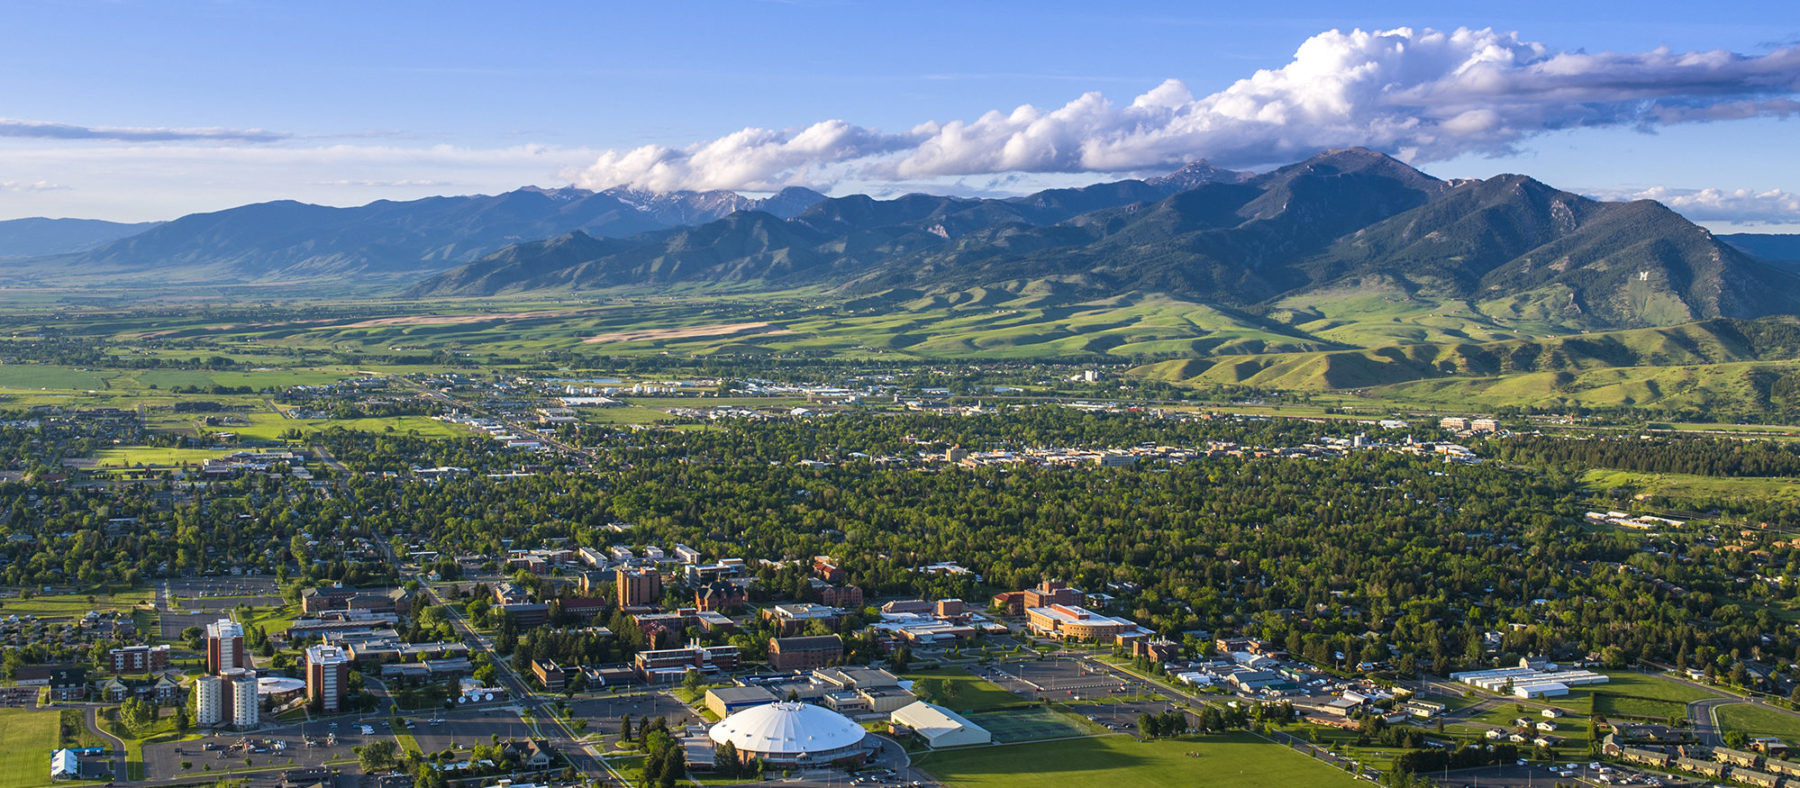
\includegraphics[width=5in,height=\textheight]{images/msu-campus.jpg}}
\usepackage{etoolbox}
\makeatletter
\providecommand{\subtitle}[1]{% add subtitle to \maketitle
  \apptocmd{\@title}{\par {\large #1 \par}}{}{}
}
\makeatother
\subtitle{Spring 2021\\
Montana State University}
\author{Melinda Yager, Jade Schmidt, Dr.~Stacey Hancock}
\date{}

\begin{document}
\maketitle

\newpage
\thispagestyle{empty}

This resource was developed by Melinda Yager, Jade Schmidt, and Stacey Hancock in 2021 to accompany the online textbook: Carnegie, N., Hancock, S., Meyer, E., Schmidt, J., and Yager, M. (2021). \emph{Montana State Introductory Statistics with R}. Montana State University. \url{https://mtstateintrostats.github.io/IntroStatTextbook/}.

This resource is released under a \href{https://creativecommons.org/licenses/by-nc-sa/4.0/}{Creative Commons BY-NC-SA 4.0} license unless otherwise noted.

\setcounter{tocdepth}{1}
\tableofcontents
\setcounter{page}{1}

\newpage

\hypertarget{preface}{%
\chapter*{Preface}\label{preface}}
\addcontentsline{toc}{chapter}{Preface}

This coursepack accompanies the textbook for STAT 216: Introduction to Statistics at Montana State University, which can be found at \url{https://mtstateintrostats.github.io/IntroStatTextbook/}. The syllabus for the course (including the course calendar), data sets, and links to D2L Brightspace, Gradescope, and the MSU RStudio server can be found on the course webpage: \url{https://math.montana.edu/courses/s216/}.
Videos assigned in the course calendar and other notes and review materials are linked in D2L.

Each of the activities in this workbook is designed to target specific learning outcomes of the course, giving you practice with important statistical concepts in a group setting with instructor guidance. In addition to the in-class activities for the course, the coursepack includes reading guides to aid in taking notes while you complete the required readings and videos. Bring this workbook with you to class each week, and take notes in the workbook as you would your own notes. A well-written complete workbook will provide an optimal study guide for exams!

The activities in this coursepack are broken into three sections: pre-class, in-class, and after class. Read through the introduction for each activity and complete the pre-class questions before attending class each week. In class, you will work through the in-class section with your group and instructor. After class, you will complete the out-of-class part of the activity.

STAT 216 is a 3-credit blended course. Rather than meeting for a total of 150 structured minutes in class per week, students meet with their instructor and cohort of classmates for 50 minutes of class per week. The other 100 minutes typically spent in class are instead spent outside of class watching instructor video lectures, reading the textbook, working through case studies, and participating in online discussion with your classmates. This structure serves two purposes: (1) enhance the safety of our community during the COVID-19 pandemic, and (2) provide additional flexibility for students to create their own schedule and make their own decisions on how they learn best.

In our experience, it takes six to nine hours per week outside of class to achieve a good grade in STAT 216 -- this means six to nine hours outside of the 150 minutes of time set aside for learning course material each week. By ``good'' we mean at least a C because a grade of C- or below does not count toward fulfilling degree requirements. Many of you set your goals higher than just getting a C, and we fully support that. You
need roughly nine hours per week to review past activities, read feedback on previous assignments, complete current assignments, and prepare for the next day's class. A typical week in the life of a STAT 216 student looks like:

\begin{itemize}
\tightlist
\item
  \emph{Prior to class meeting}:

  \begin{itemize}
  \tightlist
  \item
    Read assigned sections of the textbook, using the provided reading guides to take notes on the material.
  \item
    Watch assigned videos on that week's content, pausing to take notes and answer video quiz questions.
  \item
    Read through the introduction to the week's in-class activity and complete the pre-class questions.
  \item
    Read through the week's homework assignment and note any questions you may have on the content.
  \end{itemize}
\item
  \emph{During class meeting}:

  \begin{itemize}
  \tightlist
  \item
    Work through in-class activity with your classmates and instructor, taking detailed notes on your answers to each question in the activity.
  \end{itemize}
\item
  \emph{After class meeting}:

  \begin{itemize}
  \tightlist
  \item
    Complete the out-of-class part of the activity, plus any additional parts of the activity you did not complete in class.
  \item
    Review the posted activity solutions and wrap-up videos, and take notes on key points.
  \item
    Finish watching any remaining assigned videos or readings for the week.
  \item
    Read through the week's case study and post case study discussion posts on D2L.
  \item
    Complete the week's homework assignment.
  \end{itemize}
\end{itemize}

\hypertarget{inference-for-two-categorical-variables-hypothesis-testing}{%
\chapter{Inference for Two Categorical Variables: Hypothesis Testing}\label{inference-for-two-categorical-variables-hypothesis-testing}}

\hypertarget{reading-guide-hypothesis-testing-for-a-difference-in-proportions}{%
\section{Reading Guide: Hypothesis Testing for a Difference in Proportions}\label{reading-guide-hypothesis-testing-for-a-difference-in-proportions}}

\hypertarget{sections-5.4.1-and-5.4.2-simulation-tests-for-a-difference-in-proportions-two-sided-hypotheses}{%
\subsection*{Sections 5.4.1 and 5.4.2 (Simulation tests for a difference in proportions; Two-sided hypotheses)}\label{sections-5.4.1-and-5.4.2-simulation-tests-for-a-difference-in-proportions-two-sided-hypotheses}}
\addcontentsline{toc}{subsection}{Sections 5.4.1 and 5.4.2 (Simulation tests for a difference in proportions; Two-sided hypotheses)}

<<<<<<< HEAD
\begin{longtable}{|l|l|l|l|p{.55\textwidth}|}
\hline
\textbf{Week}& \textbf{Activity}& \textbf{Day}& \textbf{Date}& \textbf{Activity} \\ \hline
\endhead
1& 1& M& 1/11& Martian Alphabet \\*
1& 1& W& 1/13& Martian Alphabet \\*
1& 1& F& 1/15& Martian Alphabet \\ \hline
2& 2& M& 1/18& Study Design (\textit{No class}) \\*
2& 2& W& 1/20& Study Design \\*
2& 2& F& 1/22& Study Design \\ \hline
3& 3& M& 1/25& What's the Probability? \\*
3& 3& W& 1/27& What's the Probability? \\*
3& 3& F& 1/29& What's the Probability? \\ \hline
4& 4& M& 2/1& IMDb Movie Reviews \\*
4& 4& W& 2/3& IMDb Movie Reviews \\*
4& 4& F& 2/5& IMDb Movie Reviews \\ \hline
5& 4& M& 2/8& Movie Profits \\*
5& 5& W& 2/10& Movie Profits \\*	
5& 5& F& 2/12& Movie Profits \\ \hline
6& 6& M& 2/15& Handedness of Male Boxers --- Testing (\textit{No class})\\*
6& 6& W& 2/17& Handedness of Male Boxers --- Testing \\*	
6& 6& F& 2/19& Handedness of Male Boxers --- Testing \\ \hline
7& ---& M--F& 2/22--2/26& \textbf{Exam 1} \\ \hline
8& 7& M& 3/1& Handedness of Male Boxers --- Estimation \\*
8& 7& W& 3/3& Handedness of Male Boxers --- Estimation \\*	
8& 7& F& 3/5& Handedness of Male Boxers --- Estimation \\ \hline
9& 8& M& 3/8& Winter Sports Helmet Use and Head Injuries --- Testing \\*
9& 8& W& 3/10& Winter Sports Helmet Use and Head Injuries --- Testing \\*	
9& 8& F& 3/12& Winter Sports Helmet Use and Head Injuries --- Testing \\ \hline
10& 9& M& 3/15& Winter Sports Helmet Use and Head Injuries --- Estimation \\*
10& 9& W& 3/17& Winter Sports Helmet Use and Head Injuries --- Estimation \\*
10& 9& F& 3/19& Winter Sports Helmet Use and Head Injuries --- Estimation \\ \hline
11& 10& M& 3/22& COVID-19 and Air Pollution \\*
11& 10& W& 3/24& COVID-19 and Air Pollution \\*	
11& 10& F& 3/26& COVID-19 and Air Pollution \\ \hline
12& 11& M& 3/29& Weather Patterns and Record Snowfall \\*
12& 11& W& 3/31& Weather Patterns and Record Snowfall \\*
12& 11& F& 4/2& Weather Patterns and Record Snowfall  (\textit{No class})\\ \hline
13& 12& M& 4/5& Moneyball \\*
13& 12& W& 4/7& Moneyball \\*
13& 12& F& 4/9& Moneyball \\ \hline
14& ---& M--F& 4/12--4/16& \textbf{Exam 2} \\ \hline
15& ---& M--F& 4/19--4/23& Looking Ahead \\ \hline
Finals& ---& M--F& 4/26--4/30& Group Project Presentations \\ \hline
\end{longtable}
=======
\textbf{Videos}

\begin{itemize}
\tightlist
\item
  5.4
\item
  TwoPropSim
\end{itemize}

\setstretch{1.25}

\hypertarget{reminders-from-previous-sections}{%
\subsubsection*{Reminders from previous sections}\label{reminders-from-previous-sections}}
\addcontentsline{toc}{subsubsection}{Reminders from previous sections}
>>>>>>> 6902ece40b9553d6adf5f64bb69bb844cf53bb72

\(n\) = sample size

\(\hat{p}\) = sample proportion

\(\pi\) = population proportion

General steps of a hypothesis test:

\begin{enumerate}
\def\labelenumi{\arabic{enumi}.}
\item
  Frame the research question in terms of hypotheses.
\item
  Collect and summarize data using a test statistic.
\item
  Assume the null hypothesis is true, and simulate or mathematically model a null distribution for the test statistic.
\item
  Compare the observed test statistic to the null distribution to calculate a p-value.
\item
  Make a conclusion based on the p-value and write the conclusion in context.
\end{enumerate}

Parameter: a value summarizing a variable(s) for a population.

Statistic: a value summarizing a variable(s) for a sample.

Sampling distribution: plot of statistics from 1000s of samples of the same size taken from the same population.

Standard deviation of a statistic: the variability of statistics from 1000s of samples; how far, on average, each statistic is from the true value of the parameter.

Standard error of a statistic: estimated standard deviation of a statistic.

Hypothesis test: a process to determine how strong the evidence of an effect is.

\rgi Also called a `significance test'.

Simulation-based method: Simulate lots of samples of size \(n\) under assumption of the null hypothesis, then find the proportion of the simulations that are at least as extreme as the observed sample statistic.

Theory-based method: Develop a mathematical model for the sampling distribution of the statistic under the null hypothesis and use the model to calculate the probability of the observed sample statistic (or one more extreme) occurring.

Null hypothesis (\(H_0\)): the skeptical perspective; no difference; no change; no effect; random chance; what the researcher hopes to prove is \textbf{wrong}.

Alternative hypothesis (\(H_A\)): the new perspective; a difference/increase/decrease; an effect; not random chance; what the researcher hopes to prove is \textbf{correct}.

Null value: the value of the parameter when we assume the null hypothesis is true (labeled as \(parameter_0\)).

Null distribution: the simulated or modeled distribution of statistics (sampling distribution) we would expect to occur if the null hypothesis is true.

P-value: probability of seeing the observed sample data, or something more extreme, assuming the null hypothesis is true.

\(\implies\) Lower the p-value the stronger the evidence AGAINST the null hypothesis and FOR the alternative hypothesis.

Decision: a determination of whether to `reject' or `fail to reject' a null hypothesis based on a p-value and a pre-set level of significance.

Significance level (\(\alpha\)): a threshold used to determine if a p-value provides enough evidence to reject the null hypothesis or not.

\rgi Common levels of \(\alpha\) include 0.01, 0.05, and 0.10.

Statistically significant: results are considered statistically significant if the p-value is below the significance level.

\hypertarget{vocabulary}{%
\subsubsection*{Vocabulary}\label{vocabulary}}
\addcontentsline{toc}{subsubsection}{Vocabulary}

Randomization test:
\rgs

Relative risk:
\rgs

One-sided hypothesis test:
\rgs

Two-sided hypothesis test:
\rgs

\hypertarget{notes}{%
\subsubsection*{Notes}\label{notes}}
\addcontentsline{toc}{subsubsection}{Notes}

In a randomization test involving two categorical variables, how many cards will you need and how will the cards be labeled?
\rgs

Why, in the randomization test, are the cards all shuffled together and randomly dealt into two new groups?
\rgs

After shuffling, how many cards are dealt into each pile?
\rgs

Interpreting relative risk (\(RR = \frac{\hat{p_1}}{\hat{p_2}}\))

\rgi The proportion of success in group 1 is \_\_\_\_\_\_ times the proportion of success in group 2.

\rgi The proportion of success in group 1 is \_\_\_\_\_\_ \% higher/lower than in group 2.

Write the null hypothesis in notation for a test of relative risk.
\rgs

How does the p-value in a two-sided test compare to the p-value in a one-sided test?
\rgs

\hypertarget{formulas}{%
\subsubsection*{Formulas}\label{formulas}}
\addcontentsline{toc}{subsubsection}{Formulas}

Relative risk =
\rgs

\hypertarget{notation}{%
\subsubsection*{Notation}\label{notation}}
\addcontentsline{toc}{subsubsection}{Notation}

Sample size of group 1:
\rgs

Sample size of group 2:
\rgs

Sample proportion of group 1:
\rgs

Sample proportion of group 2:
\rgs

Population proportion of group 1:
\rgs

Population proportion of group 2:
\rgs

\hypertarget{example-gender-discrimination}{%
\subsubsection*{Example: Gender discrimination}\label{example-gender-discrimination}}
\addcontentsline{toc}{subsubsection}{Example: Gender discrimination}

\begin{enumerate}
\def\labelenumi{\arabic{enumi}.}
\item
  What is the research question?
  \rgs
\item
  What are the observational units?
  \rgs
\item
  What type of study design was used? Justify your answer.
  \rgs
\item
  What is the appropriate scope of inference for these data?
  \rgs
\item
  What is the sample statistic presented in this example? What notation would be used to represent this value?
  \rgs
\item
  What is the parameter representing in the context of this problem? What notation would be used to represent this parameter?
  \rgs
  \rgs
\item
  Write the null and the alternative hypotheses in words.
  \rgs
  \rgs
\item
  Write the null and the alternative hypotheses in notation.
  \rgs
\item
  How could we use cards to simulate \textbf{1} sample \emph{which assumes the null hypothesis is true}? How many blue cards --- to represent what? How many red cards --- to represent what? What would we do with the cards? What would you record once you have a simulated sample?
  \rgs
  \rgs
\item
  How can we calculate a p-value from the simulated null distribution for this example?
  \rgs
  \rgs
\item
  What was the p-value of the test?
  \rgs
\item
  At the 5\% significance level, what decision would you make?
  \rgs
\item
  What conclusion should the researcher make?
  \rgs
  \rgs
\item
  Are the results in this example statistically significant? Justify your answer.
  \rgs
\end{enumerate}

\hypertarget{example-opportunity-cost}{%
\subsubsection*{Example: Opportunity cost}\label{example-opportunity-cost}}
\addcontentsline{toc}{subsubsection}{Example: Opportunity cost}

\begin{enumerate}
\def\labelenumi{\arabic{enumi}.}
\item
  What is the research question?
  \rgs
\item
  What are the observational units?
  \rgs
\item
  What type of study design was used? Justify your answer.
  \rgs
\item
  What is the appropriate scope of inference for these data?
  \rgs
\item
  What is the sample statistic presented in this example? What notation would be used to represent this value?
  \rgs
\item
  What is the parameter representing in the context of this problem? What notation would be used to represent this parameter?
  \rgs
  \rgs
\item
  Write the null and the alternative hypotheses in words.
  \rgs
  \rgs
\item
  Write the null and the alternative hypotheses in notation.
  \rgs
\item
  How could we use cards to simulate \textbf{1} sample \emph{which assumes the null hypothesis is true}? How many blue cards --- to represent what? How many red cards --- to represent what? What would we do with the cards? What would you record once you have a simulated sample?
  \rgs
  \rgs
\item
  How can we calculate a p-value from the simulated null distribution for this example?
  \rgs
  \rgs
\item
  What was the p-value of the test?
  \rgs
\item
  Interpret the p-value in the context of the problem.
  \rgs
  \rgs
\item
  At the 5\% significance level, what decision would you make?
  \rgs
\item
  What conclusion should the researcher make?
  \rgs
\item
  Are the results in this example statistically significant? Justify your answer.
  \rgs
\end{enumerate}

\hypertarget{example-cpr-and-blood-thinner}{%
\subsubsection*{Example: CPR and blood thinner}\label{example-cpr-and-blood-thinner}}
\addcontentsline{toc}{subsubsection}{Example: CPR and blood thinner}

\begin{enumerate}
\def\labelenumi{\arabic{enumi}.}
<<<<<<< HEAD
\setcounter{enumi}{4}
\tightlist
\item
  Is the variable identified in question 4 categorical or quantitative?
\end{enumerate}

\vspace{0.3in}

\textbf{Step 3}: Once we have collected data, the next step is to \emph{summarize and visualize the data}.

\begin{enumerate}
\def\labelenumi{\arabic{enumi}.}
\setcounter{enumi}{5}
\tightlist
\item
  How many people in your class were correct in identifying Bumba? Using the class size from question 3, calculate the proportion of students who correctly identified Bumba.
\end{enumerate}

\begin{center}
$\mbox{proportion} = \frac{\mbox{number of students who correctly identified Bumba}}{\mbox{total number of students}}$
\end{center}

\vspace{0.7in}

The proportion in question 6 is called a \textbf{summary statistic}---a single value that summarizes the data set. It is important to note that a variable is different than a summary statistic. A \emph{variable} is measured on a \emph{single observational unit} while a summary statistic is calculated from a group of observational units. For example, the variable ``whether or not a student lives on campus'' can be measured on each individual student. In a class of 50 students we can calculate the proportion of students who live on campus, the summary statistic. Look back and make sure you wrote the variable in question 4 as a variable, NOT a summary statistic.

Looking at the data set and the summary statistic is only one way to display the data. We will also want to create a visualization or picture of the data. A \textbf{frequency bar plot} is used to display categorical data as a count or frequency. Since our variable has two levels or outcomes, correct or incorrect, we will create two bars---one for each level.

\begin{enumerate}
\def\labelenumi{\arabic{enumi}.}
\setcounter{enumi}{6}
\tightlist
\item
  Plot the observed class data using a frequency bar plot. Be sure to add a scale to the y-axis.
\end{enumerate}

\begin{center}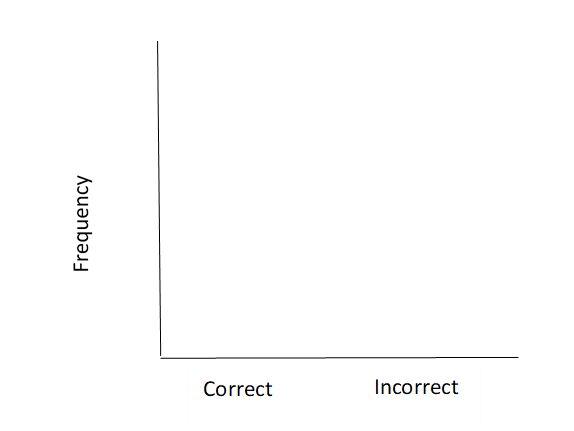
\includegraphics[width=0.4\linewidth]{images/barplot_martian} \end{center}

We can also visualize the data as a proportion in a \textbf{relative frequency bar plot}. Relative frequency is the proportion calculated for each level of the categorical variable.

\begin{enumerate}
\def\labelenumi{\arabic{enumi}.}
\setcounter{enumi}{7}
\tightlist
\item
  Plot the observed class data using a relative frequency bar plot. Be sure to add a scale to the y-axis.
\end{enumerate}

\begin{center}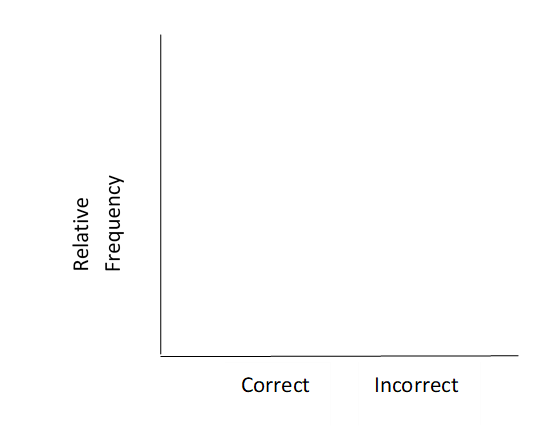
\includegraphics[width=0.4\linewidth]{images/relative_barplot_martian} \end{center}

\textbf{Step 4}: The next step is to \emph{use statistical analysis methods to draw inferences from the data}. To answer the research question, we will simulate what \emph{could} have happened in our class given random chance, repeat many times to understand the expected \emph{variability} between different ``randomly guessing'' classes, then compare our class's observed data to the simulation. This gives us an estimate of how often (or the probability of) the class's result would occur if students were all merely guessing, allowing us to determine if the data provides evidence that we as a class can in fact read Martian.

\newpage

\begin{enumerate}
\def\labelenumi{\arabic{enumi}.}
\setcounter{enumi}{8}
\item
  If humans really don't know Martian and are just guessing which is Bumba, what are the chances of getting it right?
  \vspace{0.3in}

  How could we use a coin to simulate each student ``just guessing'' which Martian letter is Bumba?
  \vspace{.9in}

  How could we use coins to simulate the entire class ``just guessing'' which Martian letter is Bumba?
  \vspace{.9in}

  How many people in your class would you expect to choose Bumba correctly just by chance? Explain your reasoning.
  \vspace{.9in}
\item
  Each student will flip a coin one time to simulate your ``guess'' under the assumption that we can't read Martian. Let Heads = correct, Tails = incorrect. What was the result of your one simulation?
  \vspace{.3in}

  What was the result from your class's simulation? What proportion of students ``guessed'' correctly in the simulation?
  \vspace{.5in}
\item
  If students really don't know Martian and are just guessing which is Bumba, which seems more unusual: the result from your class's \textbf{simulation} or the observed proportion of students in your class that were correct (this is your summary statistic from question 6)? Explain your reasoning.
\end{enumerate}

\newpage

\begin{enumerate}
\def\labelenumi{\arabic{enumi}.}
\setcounter{enumi}{11}
\tightlist
\item
  While your observed class data is likely far different from the simulated ``just-guessing'' class, comparing our class data to a single simulation does not provide enough information. The differences seen could just be due to the randomness of that set of coin flips! Let's simulate another class. Each student should flip their coin again. What was the result from your class's second simulation? What proportion of students ``guessed'' correctly in the second simulation? Create a plot to compare the two simulated results with the observed class result.
\end{enumerate}

\vspace{1in}

\begin{enumerate}
\def\labelenumi{\arabic{enumi}.}
\setcounter{enumi}{12}
\tightlist
\item
  We still only have a couple of simulations to compare our class data to. It would be much better to be able to see how our class compared to hundreds or thousands of ``just-guessing'' classes. Since we don't want to flip coins all class period, your instructor will use a computer simulation to get 1000 trials. Fill in the following blanks to describe how we would create a simulation of random guessing with 1000 trials (repetitions).
\end{enumerate}

~~~~~~~~~~Probability of correct guesses: \_\_\_\_\_

\vspace{0.05in}

~~~~~~~~~~Sample size: \_\_\_\_\_

\vspace{0.05in}

~~~~~~~~~~Number of repetitions: \_\_\_\_\_

\vspace{0.05in}

\begin{enumerate}
\def\labelenumi{\arabic{enumi}.}
\setcounter{enumi}{13}
\tightlist
\item
  Sketch the distribution displayed by your instructor here. Label each axis appropriately.
\end{enumerate}

\vspace{1.5in}

\begin{enumerate}
\def\labelenumi{\arabic{enumi}.}
\setcounter{enumi}{14}
\tightlist
\item
  Is your class particularly good or bad at Martian? Use the plot in question 14 to explain your answer.
\end{enumerate}

\vspace{.5in}

\begin{enumerate}
\def\labelenumi{\arabic{enumi}.}
\setcounter{enumi}{15}
\tightlist
\item
  Is it \emph{possible} that we could see our class results just by chance if everyone was just guessing? Explain your reasoning.
\end{enumerate}

\vspace{.5in}

\begin{enumerate}
\def\labelenumi{\arabic{enumi}.}
\setcounter{enumi}{16}
\tightlist
\item
  Is it \emph{likely} that we could see our class results just by chance if everyone was just guessing? Explain your reasoning.
\end{enumerate}

\newpage

\textbf{Step 5}: The next step in the statistical investigation process is to \emph{communicate the results and answer the research question}.

\begin{enumerate}
\def\labelenumi{\arabic{enumi}.}
\setcounter{enumi}{17}
\tightlist
\item
  Does this activity provide strong evidence that students were not just guessing at random? If so, what do you think is going on here? Can we as a class read Martian?\footnote{Reference for ``Martian alphabet'' is a TED talk given by Vilayanur Ramachandran in 2007. The synesthesia part begins at roughly 17:30 minutes: \texttt{http://www.ted.com/talks/vilayanur\_ramachandran\_on\_your\_mind}.}
\end{enumerate}

\vspace{1in}

\textbf{Step 6}: The final step of any statistical investigation is to \emph{revisit and look ahead}.

\begin{enumerate}
\def\labelenumi{\arabic{enumi}.}
\setcounter{enumi}{18}
\tightlist
\item
  Can you think of any limitations of our study? Can you think of a new topic that might be of interest based on the results of our study?
\end{enumerate}

\vspace{1in}

\newpage

\hypertarget{out-of-class-activity}{%
\subsection{Out-of-class activity}\label{out-of-class-activity}}

Since this class is taught in a blended format, we are only in class one day per week. During class we will complete the in-class activity from the course pack. Outside of class, students will read from the textbook, watch course videos, and complete an out-of-class activity on the other two days of class. To become familiar with the course outline, read through the syllabus, \url{https://mtstateintrostats.github.io/Syllabus/}, your day specific cohort calendar, and watch the Stat 216 Course Tour on D2L before answering the following questions.

\begin{enumerate}
\def\labelenumi{\arabic{enumi}.}
\tightlist
\item
  When are the case study discussion posts due on D2L each week?
\end{enumerate}

\vspace{0.3in}

\begin{enumerate}
\def\labelenumi{\arabic{enumi}.}
\setcounter{enumi}{1}
\tightlist
\item
  For your cohort, what day and time are the weekly assignments due on Gradescope?
\end{enumerate}

\vspace{0.3in}

\begin{enumerate}
\def\labelenumi{\arabic{enumi}.}
\setcounter{enumi}{2}
\tightlist
\item
  For your cohort, when is Exam 1? Exam 2?
\end{enumerate}

\vspace{0.3in}

\hypertarget{introduction-to-r}{%
\subsubsection{\texorpdfstring{Introduction to \texttt{R}}{Introduction to R}}\label{introduction-to-r}}

In Stat 216 we will use the statistical package \texttt{R} to analyze data through the IDE (integrated development environment) RStudio. Though it is possible to download \texttt{R} and RStudio on your own computer, we will use this program through the MSU RStudio server: \url{https://rstudio.math.montana.edu/}.

Read through the preliminaries chapter in the textbook and watch the video ``Starting with \texttt{R}'' before completing the following questions.

The RStudio workflow operates best by the use of ``Projects''. You should create a separate project for each activity or assignment in this course that requires the use of \texttt{R}. To get started with this activity, follow these steps:

\begin{itemize}
\tightlist
\item
  Log onto the RStudio server using your NetID and password: \url{https://rstudio.math.montana.edu/}.
\item
  In the top right corner, you will see a dropdown menu next to ``Project'' that currently says ``(None)''. Click on this menu and choose ``New Project''. (Alternatively, you can click the ``File'' menu in the top left and select ``New Project''.)

  \begin{itemize}
  \tightlist
  \item
    A ``New Project Wizard'' window should pop up: click ``New Directory'', then click ``New Project''.
  \item
    Give your project directory a name (e.g., Activity1). \emph{Do not use spaces or other characters in the name.}
  \item
    Click ``Browse'' and choose a location where you would like to save your project (you can create a new folder if desired). Note that this location is on your server account, not on your computer.
  \item
    Leave all other boxes unchecked, and click ``Create Project''. (Now, if you click on the home icon in the top right, you will see your RStudio account, and the project should be listed under ``Projects''.)
  \end{itemize}
\item
  Download the Martian Alphabet \texttt{R} script file from D2L.
\item
  Click ``Upload'' in the ``Files'' tab in the bottom right window of RStudio. Click ``Choose File'', and navigate to the folder where the Martian Alphabet \texttt{R} script file is saved. Then click ``Open''; then click ``Ok''.
\item
  You should see the uploaded file appear in the list of files. Click on the filename to open the file.
\end{itemize}

In the Martian Alphabet \texttt{R} script file, highlight all of the lines of code that start with \texttt{library} and click ``Run''. This will load the \textbf{packages} (or libraries) needed for this course; each package is a collection of \texttt{R} functions. We review a few of these packages here.

\begin{itemize}
\tightlist
\item
  Throughout the semester we will use the package \texttt{tidyverse} to allow us to use chaining (see Section 1.7 in the textbook for more on this symbol \texttt{\%\textgreater{}\%}.) Contained in \texttt{tidyverse} is the package \texttt{ggplot2}, used to create graphs in RStudio.
\item
  The package \texttt{mosaic} contains the \texttt{favstats} function to find summary statistics for quantitative variables.
\item
  We will use the package \texttt{catstats}, starting in Chapter 5, to create simulations for statistical inference.
\end{itemize}

These packages are already installed in the RStudio server, but you need to use the \texttt{library} function to call the package into your R environment.

The \# sign is not part of the \texttt{R} code.
It is used by these authors to add comments to the \texttt{R} code and explain what each call is telling the program to do.
\texttt{R} will ignore everything after a \# sign when executing the code.

In the Martian Alphabet \texttt{R} script file for the \texttt{one\_proportion\_test} function arguments, enter your class size (Q3 from the in-class activity) for \texttt{sample\_size} and the number of students who were correct in identifying Bumba (Q6 from the in-class activity) for \texttt{as\_extreme\_as} argument. Highlight these lines and click run.

\begin{enumerate}
\def\labelenumi{\arabic{enumi}.}
\setcounter{enumi}{3}
\tightlist
\item
  Is the distribution created from this code similar to what you saw in class in Q14?
\end{enumerate}

\vspace{0.3in}

\hypertarget{take-home-messages}{%
\subsection{Take-home messages}\label{take-home-messages}}

\begin{enumerate}
\def\labelenumi{\arabic{enumi}.}
\item
  In this course we will learn how to evaluate a claim by comparing observed results (classes' ``guesses'' when asked to identify Bumba) to a distribution of many simulated results under an assumption like ``blind guessing.''
\item
  Blind guessing between two outcomes will be correct only about half the time. We can simulate data using a computer program to fit the assumption of blind guessing.
\item
  Unusual observed results will make us doubt the assumptions used to create the simulated distribution. A large number of correct ``guesses'' is evidence that a person was not just blindly guessing.
\end{enumerate}

\hypertarget{additional-notes}{%
\subsection{Additional notes}\label{additional-notes}}

Use this space to summarize your thoughts and take additional notes on this week's activity and material covered, and to write down the names and contact information of your teammates.

\hypertarget{study-design}{%
\chapter{Study Design}\label{study-design}}

\hypertarget{reading-guide-sampling-experimental-design-and-scope-of-inference}{%
\section{Reading Guide: Sampling, Experimental Design, and Scope of Inference}\label{reading-guide-sampling-experimental-design-and-scope-of-inference}}

\hypertarget{section-1.3-sampling-principles-and-strategies}{%
\subsection*{Section 1.3 (Sampling principles and strategies)}\label{section-1.3-sampling-principles-and-strategies}}
\addcontentsline{toc}{subsection}{Section 1.3 (Sampling principles and strategies)}

\textbf{Videos}

\begin{itemize}
\tightlist
\item
  1.3
\end{itemize}

\setstretch{1.25}

\hypertarget{vocabulary}{%
\subsubsection*{Vocabulary}\label{vocabulary}}
\addcontentsline{toc}{subsubsection}{Vocabulary}

(Target) Population:
\rgs

Sample:
\rgs

Anecdotal evidence:
\rgs

Bias:
\rgs

\rgi Selection bias:
\rgs

\rgi Non-response bias:
\rgs

\rgi Response bias:
\rgs

Convenience sample:
\rgs

Simple Random Sample:
\rgs

Non-response rate:
\rgs

Representative:
\rgs

\hypertarget{notes}{%
\subsubsection*{Notes}\label{notes}}
\addcontentsline{toc}{subsubsection}{Notes}

Ideally, how should we sample cases from our target population? Using what sampling method?
\rgs

\hypertarget{notes-on-types-of-sampling-bias}{%
\paragraph{Notes on types of sampling bias}\label{notes-on-types-of-sampling-bias}}
\addcontentsline{toc}{paragraph}{Notes on types of sampling bias}

\begin{itemize}
\item
  Someone must first be \emph{chosen} to be in a study and refuse to participate in order to have \textbf{non-response bias}.
\item
  There must be a valid reason for someone to lie or be untruthful to justify saying \textbf{response bias} is present. Yes, anyone could lie at any time to any question. Response bias is when those lies are predictable and systematic based on outside influences.
  \rgs
\end{itemize}

True or False: Convenience sampling tends to result in non-response bias.

True or False: Volunteer sampling tends to result in response bias.

True or False: Random sampling helps to resolve selection bias, but has no impact on non-response or response bias.

\hypertarget{sections-1.4-observational-studies-1.5-experiments-and-1.6-scope-of-inference}{%
\subsection*{Sections 1.4 (Observational studies), 1.5 (Experiments), and 1.6 (Scope of inference)}\label{sections-1.4-observational-studies-1.5-experiments-and-1.6-scope-of-inference}}
\addcontentsline{toc}{subsection}{Sections 1.4 (Observational studies), 1.5 (Experiments), and 1.6 (Scope of inference)}

\setstretch{1}

\textbf{Videos}

\begin{itemize}
\tightlist
\item
  1.4to1.6
\end{itemize}

\setstretch{1.25}

\hypertarget{reminders-from-section-1.2}{%
\subsubsection*{Reminders from Section 1.2}\label{reminders-from-section-1.2}}
\addcontentsline{toc}{subsubsection}{Reminders from Section 1.2}

\textbf{Explanatory variable}: The variable researchers think \emph{may be} effecting the other variable. What the researchers control/assign in an experiment. If comparing groups, the explanatory variable puts the observational units into groups.

\textbf{Response variable}: The variable researchers think \emph{may be} influenced by the other variable. This variable is always observed, never controlled or assigned.

\hypertarget{vocabulary-1}{%
\subsubsection*{Vocabulary}\label{vocabulary-1}}
\addcontentsline{toc}{subsubsection}{Vocabulary}

Observational study:
\rgs

\rgi Observational data:
\rgs

\rgi Prospective study:
\rgs

\rgi Retrospective study:
\rgs

Confounding variable:
\rgs

Experiment:
\rgs

\rgi Randomized experiment:
\rgs

\rgi Blocking:
\rgs

\rgi Treatment group:
\rgs

\rgi Control group:
\rgs

\rgi Placebo:
\rgs

\rgi Placebo effect:
\rgs

\rgi Blinding:
\rgs

Scope of inference:
\rgs

Generalizability:
\rgs

Causation:
\rgs

\hypertarget{notes-1}{%
\subsubsection*{Notes}\label{notes-1}}
\addcontentsline{toc}{subsubsection}{Notes}

What are the four principles of a well-designed randomized experiment?\\
\rgs
\rgs
\rgs

Fill in the appropriate scope of inference for each study design.

\begin{center}
\begin{tabular}{|p{2in}|p{2in}|p{2in}|}
\hline
 & \multicolumn{2}{|c|}{\textbf{Study Type}} \\ \hline
 \textbf{Selection of Cases} & Randomized experiment & Observational study \\ \hline
 Random sample && \\ 
 (and no other sampling bias) & & \\ 
  & & \\
   & & \\ \hline
   Non-random sample && \\ 
   (or other sampling bias) & & \\ 
  & & \\
   & & \\ \hline
\end{tabular}
\end{center}

\rgs

True or False: Observational studies can show an association between two variables, but cannot determine a causal relationship.

True or False: In order for an experiment to be valid, a placebo must be used.

True or False: If random sampling of the target population is used, and no other types of bias are suspected, results from the sample can be generalized to the entire target population.

True or False: If random sampling of the target population is used, and no other types of bias are suspected, results from the sample can be inferred as a causal relationship between the explanatory and response variables.

\newpage

\hypertarget{activity-study-design}{%
\section{Activity: Study Design}\label{activity-study-design}}

\setstretch{1}

\hypertarget{learning-outcomes}{%
\subsection{Learning outcomes}\label{learning-outcomes}}

\begin{itemize}
\item
  Explain the purpose of random sampling and its effect on scope of inference.
\item
  Explain the purpose of random assignment and its effect on scope of inference.
\item
  Identify whether a study design is observational or an experiment.
\item
  Identify confounding variables in observational studies and explain why they are confounding.
\item
  Identify the types of bias present in a study.
\end{itemize}

\hypertarget{terminology-review}{%
\subsection{Terminology review}\label{terminology-review}}

In this week's activity, we will examine different types of sampling bias and study designs, confounding variables, and how to determine the scope of inference for a study. Some terms covered in this activity are:

\begin{itemize}
\item
  Population
\item
  Sample
\item
  Parameter
\item
  Statistic
\item
  Selection bias
\item
  Response bias
\item
  Non-response bias
\item
  Scope of inference
\item
  Explanatory variable
\item
  Response variable
\item
  Confounding variable
\item
  Experiment
\item
  Observational study
\end{itemize}

To review these concepts, see Sections 1.3 through 1.6 in the textbook.

\newpage

\hypertarget{types-of-sampling-bias.-complete-q1-before-class.}{%
\subsection{Types of sampling bias. Complete Q1 before class.}\label{types-of-sampling-bias.-complete-q1-before-class.}}

There are two parts to study design: how the sample was selected and how the study was conducted. First, we will look at sampling and types of bias (selection, non-response, or response).

In these next questions, identify the target population, the sample selected, the variable, and the type of bias present.

\begin{enumerate}
\def\labelenumi{\arabic{enumi}.}
\item
  To determine if the proportion of out-of-state undergraduate students at Montana State University has increased in the last 10 years, a statistics instructor sent an email survey to 500 randomly selected current undergraduate students. One of the questions on the survey asked whether they had in-state or out-of-state residency. She only received 378 responses.
  \vspace{0.25in}

  Target population:
  \vspace{0.3in}

  Sample:
  \vspace{0.3in}

  Variable:
  \vspace{0.3in}

  Type(s) of bias:
  \vspace{0.3in}
\item
  Recently, a survey was conducted to assess current presidential approval in the United States. A random sample of 6395 US adults was taken. One of the questions asked in the survey was, ``Do you agree or disagree with the President on many or nearly all of the top issues facing the country today?'' Of those surveyed, 42\% said they did agree.
  \vspace{0.25in}

  Target population:
  \vspace{0.3in}

  Sample:
  \vspace{0.3in}

  Variable:
  \vspace{0.3in}

  Type(s) of bias:
  \vspace{0.3in}
\end{enumerate}

\newpage

\begin{enumerate}
\def\labelenumi{\arabic{enumi}.}
\setcounter{enumi}{2}
\item
  A television station is interested in predicting whether or not a local referendum to legalize marijuana for adult use will pass. It asks its viewers to phone in and indicate whether they are in favor or opposed to the referendum. Of the 2241 viewers who phoned in, forty-five percent were opposed to legalizing marijuana.
  \vspace{0.1in}

  Target population:
  \vspace{0.3in}

  Sample:
  \vspace{0.3in}

  Variable:
  \vspace{0.3in}

  Type(s) of bias:
  \vspace{0.3in}
\item
  To gauge the interest in a new swimming pool, a local organization stood outside of the Bogart Pool in Bozeman, MT, during open hours. One of the questions they asked was, ``Since the Bogart Pool is in such bad repair, don't you agree that the city should fund a new pool?''
  \vspace{0.1in}

  Target population:
  \vspace{0.3in}

  Sample:
  \vspace{0.3in}

  Variable:
  \vspace{0.3in}

  Type(s) of bias:
  \vspace{0.3in}
\end{enumerate}

\newpage

\hypertarget{study-design-1}{%
\subsection{Study design}\label{study-design-1}}

The two main study designs we will cover are \textbf{observational studies} and \textbf{experiments}. Both the sampling method and the study design will help to determine the \textbf{scope of inference} for a study: To whom can we generalize, and can we conclude causation or only association? Remember that only in a randomized experiment can we conclude a \textbf{causal} (cause and effect) relationship between the explanatory and response variable.

\begin{center}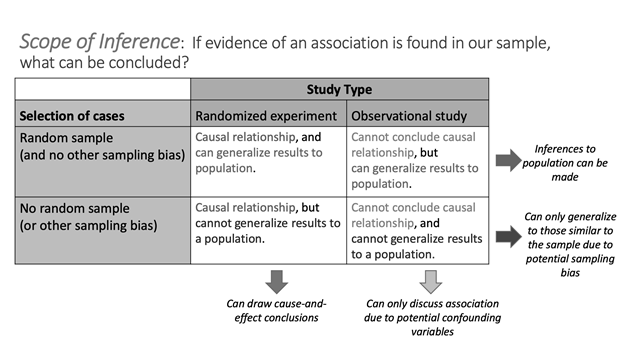
\includegraphics[width=0.75\linewidth]{images/ScopeOfInferenceGreyscale} \end{center}

For the next exercises, identify the explanatory variable, the response variable, the study design (observational study or experiment), and the scope of inference (using the above chart).

\begin{enumerate}
\def\labelenumi{\arabic{enumi}.}
\setcounter{enumi}{4}
\item
  The pharmaceutical company Moderna Therapeutics, working in conjunction with the National Institutes of Health, conducted Phase 3 clinical trials towards a vaccine for COVID-19 last fall. US clinical research sites enrolled 30,000 volunteers without COVID-19 to participate. Participants were randomly assigned to receive either the candidate vaccine or a saline placebo. They were then followed to assess whether or not they developed COVID-19. The trial was double-blind, so neither the investigators nor the participants knew who was assigned to which group.
  \vspace{0.1in}

  Explanatory variable:
  \vspace{0.25in}

  Response variable:
  \vspace{0.25in}

  Study design:
  \vspace{0.25in}

  What is the scope of inference for this study?
  \vspace{0.5in}
\end{enumerate}

\newpage

\begin{enumerate}
\def\labelenumi{\arabic{enumi}.}
\setcounter{enumi}{5}
\item
  In another study, a local health department randomly selected 1000 US adults without COVID-19 to participate in a health survey. Each participant was assessed at the beginning of the study and then followed for one year. They were interested to see which participants elected to receive a vaccination for COVID-19 and whether any participants developed COVID-19.
  \vspace{0.1in}

  Explanatory variable:
  \vspace{0.25in}

  Response variable:
  \vspace{0.25in}

  Study design:
  \vspace{0.25in}

  What is the scope of inference for this study?
  \vspace{0.5in}
\end{enumerate}

A \textbf{confounding variable} is a variable that is \emph{both}

\begin{enumerate}
\def\labelenumi{\arabic{enumi}.}
\tightlist
\item
  associated with the explanatory variable, \emph{and}
\item
  associated with the response variable.
\end{enumerate}

When both these conditions are met, if we observe an association between the explanatory variable and the response variable in the data, we cannot be sure if this association is due to the explanatory variable or the confounding variable---the explanatory and confounding variables are ``confounded.''

\begin{center}\includegraphics[width=0.4\linewidth]{02-study-design_files/figure-latex/unnamed-chunk-2-1} \end{center}

\begin{enumerate}
\def\labelenumi{\arabic{enumi}.}
\setcounter{enumi}{6}
\tightlist
\item
  For each of the studies in questions 5 and 6, determine whether confounding variables could be an issue. If so, identify a potential confounding variable and explain how it meets the definition of a confounding variable.
  \vspace{1.5in}
\end{enumerate}

\newpage

\hypertarget{out-of-class-activity}{%
\subsection{Out-of-class activity}\label{out-of-class-activity}}

In the in-class activity, we looked at sampling methods and study design. Here are a few more questions to review that material.

\begin{enumerate}
\def\labelenumi{\arabic{enumi}.}
\item
  The Bozeman school district is interested in surveying parents of students about their opinions on returning to in-person classes following the COVID-19 pandemic. They divided the school district into 10 divisions based on location and randomly surveyed 20 households within each division. Explain why selection bias would be present in this study design.
  \vspace{1in}
\item
  A study published in 2007 by Christopher Johnson, professor of music education and music therapy at the University of Kansas, revealed that students in elementary schools with superior music education programs scored around 20 percent higher in math scores on standardized tests, compared to schools with low-quality music programs. Explain how school budget could be a potential confounding variable. Be sure to address how the confounding variable is related to both the explanatory and response variable.
\end{enumerate}

\vspace{1in}

\begin{enumerate}
\def\labelenumi{\arabic{enumi}.}
\setcounter{enumi}{2}
\tightlist
\item
  What is the purpose of random selection of a sample from the population?
\end{enumerate}

\vspace{0.8in}

\begin{enumerate}
\def\labelenumi{\arabic{enumi}.}
\setcounter{enumi}{3}
\tightlist
\item
  What is the purpose of random assignment of the cases in a study to the explanatory variable groups?
\end{enumerate}

\vspace{0.8in}

\hypertarget{take-home-messages}{%
\subsection{Take-home messages}\label{take-home-messages}}

\begin{enumerate}
\def\labelenumi{\arabic{enumi}.}
\item
  If the sample is selected using a random and non-biased method of selection (i.e., a random sample of the target population with no response or non-response bias), then the results of the study can be generalized to the target population. When using biased methods of selection, the results only apply to the sample selected or similar observational units.
\item
  The study design determines if we can draw causal inferences or not. If an association is detected, a randomized experiment allows us to conclude that there is a causal (cause-and-effect) relationship between the explanatory and response variable. Observational studies have potential confounding variables within the study that prevent us from inferring a causal relationship between the variables.
\item
  Confounding variables are variables not included in the study that are related to both the explanatory and the response variables. When there are potential confounding variables in the study we cannot draw causal inferences.
\end{enumerate}

\hypertarget{additional-notes}{%
\subsection{Additional notes}\label{additional-notes}}

Use this space to summarize your thoughts and take additional notes on this week's activity and material covered.

\hypertarget{exploring-categorical-data}{%
\chapter{Exploring Categorical Data}\label{exploring-categorical-data}}

\hypertarget{reading-guide-introduction-to-r-categorical-data-and-probability}{%
\section{\texorpdfstring{Reading Guide: Introduction to \texttt{R}, Categorical Data, and Probability}{Reading Guide: Introduction to R, Categorical Data, and Probability}}\label{reading-guide-introduction-to-r-categorical-data-and-probability}}

\hypertarget{section-1.7-data-in-r}{%
\subsection*{\texorpdfstring{Section 1.7 (Data in \texttt{R})}{Section 1.7 (Data in R)}}\label{section-1.7-data-in-r}}
\addcontentsline{toc}{subsection}{Section 1.7 (Data in \texttt{R})}

\textbf{Videos}

\begin{itemize}
\tightlist
\item
  Starting\_with\_R
\end{itemize}

\setstretch{1.25}

\hypertarget{notes}{%
\subsubsection*{Notes}\label{notes}}
\addcontentsline{toc}{subsubsection}{Notes}

\texttt{R} is case sensitive, meaning it reads \texttt{data} differently from \texttt{Data}. If you get an error message, check that your capitalization is correct.

\texttt{R} does not like spaces or special characters This means the column and row headers in the data set should not have spaces, periods, commas, etc. Instead of titling the variable \texttt{column\ header}, use \texttt{column\_header} or \texttt{ColumnHeader}.

\textbf{Tidy data}: Data frames with

\rgi 1 row per \_\_\_\_\_\_\_\_\_\_\_\_\_\_\_\_,

\rgi 1 column per \_\_\_\_\_\_\_\_\_\_\_\_.

We highly recommend completing Tutorial 1 at the end of Chapter 1 (all four lessons) to give you practice with R/RStudio AND to help reflect on the content of Chapter 1: basics of data, sampling, study design, and scope of inference. These tutorials have some content questions and some places for you to practice using R online with some guidance.

\rgi \_\_ indicate spots you need to type in functions, data sets, or variable names.

\rgi There are Hint and Solution buttons on the R code box to help you.

We would not expect you to know the coding right now, especially for things like mutations or creating new variables in the data set. But seeing some initial coding for these more difficult functions will only make you more comfortable using the functions we will use in this course!

\hypertarget{functions}{%
\subsubsection*{Functions}\label{functions}}
\addcontentsline{toc}{subsubsection}{Functions}

State what these introductory functions do in \texttt{R}:

\texttt{glimpse(data\_set\_name)}

\texttt{head(data\_set\_name)}

\texttt{data\_set\_name\$variable}

\texttt{\%\textgreater{}\%}

\texttt{\textless{}-}

\hypertarget{section-2.1-exploring-categorical-data}{%
\subsection*{Section 2.1 (Exploring categorical data)}\label{section-2.1-exploring-categorical-data}}
\addcontentsline{toc}{subsection}{Section 2.1 (Exploring categorical data)}

\setstretch{1}

\textbf{Videos}

\begin{itemize}
\tightlist
\item
  2.1
\item
  MosaicPlots
\end{itemize}

\setstretch{1.25}

\hypertarget{vocabulary}{%
\subsubsection*{Vocabulary}\label{vocabulary}}
\addcontentsline{toc}{subsubsection}{Vocabulary}

Frequency table:
\rgs

Relative frequency table:
\rgs

Contingency or Two-way table:
\rgs

Unconditional proportion:
\rgs

Conditional proportion:
\rgs

\rgi Row proportions:
\rgs

\rgi Column proportions:
\rgs

Statistic:
\rgs

\rgi Sample proportion:
\rgs

\rgi \rgi Notation:
\rgs

Parameter:
\rgs

\rgi Population proportion:
\rgs

\rgi \rgi Notation:
\rgs

Bar plot:
\rgs

Segmented bar plot:
\rgs

Simpson's Paradox:
\rgs

\hypertarget{notes-1}{%
\subsubsection*{Notes}\label{notes-1}}
\addcontentsline{toc}{subsubsection}{Notes}

In a contingency table, which variable (explanatory or response) generally will make the columns of the table? Which variable on the rows?
\rgs

In a segmented bar plot, the bars represent the levels of which variable? The segments represent the levels of which variable?
\rgs

What type of plot(s) are appropriate to display a single categorical variable?
\rgs

What type of plot(s) are appropriate to display two categorical variables?
\rgs

What is the difference between a standardized segmented bar plot and a mosaic plot?
\rgs

True or false: Pie charts are generally highly recommended ways to graphically display categorical data.

True or false: Two categorical variables are associated if the conditional proportions of a particular outcome (typically of the response variable) differ across levels of the other variable (typically the explanatory).

True or false: When a segmented bar plot has segments that sum to 1 (or 100\%), the segment heights correspond to the proportions conditioned on the \textbf{segment}.

\hypertarget{review-of-simpsons-paradox}{%
\subsubsection*{Review of Simpson's Paradox}\label{review-of-simpsons-paradox}}
\addcontentsline{toc}{subsubsection}{Review of Simpson's Paradox}

Based on the segmented bar plot in Figure 2.6, which race of defendant was more likely to have the death penalty invoked?
\rgs

Based on the segmented bar plot in Figure 2.7 and Table 2.9, which race of defendant was more likely to have the death penalty invoked when the victim was Caucasian?
\rgs

Based on the segmented bar plot in Figure 2.7 and Table 2.9, which race of defendant was more likely to have the death penalty invoked when the victim was African American?
\rgs

The direction of the relationship between the \_\_\_\_\_\_\_\_\_\_\_\_\_\_
and \_\_\_\_\_\_\_\_\_\_\_\_\_\_ variables is \textbf{reversed} when accounting for
a \_\_\_\_\_\_\_\_\_\_\_\_\_\_ variable.
\rgs

\hypertarget{section-2.2-probability-with-tables}{%
\subsection*{Section 2.2 (Probability with tables)}\label{section-2.2-probability-with-tables}}
\addcontentsline{toc}{subsection}{Section 2.2 (Probability with tables)}

\setstretch{1}

\textbf{Videos}

\begin{itemize}
\tightlist
\item
  2.2
\end{itemize}

\setstretch{1.25}

\hypertarget{vocabulary-1}{%
\subsubsection*{Vocabulary}\label{vocabulary-1}}
\addcontentsline{toc}{subsubsection}{Vocabulary}

Random process:
\rgs

Probability:
\rgs

Hypothetical two-way table:
\rgs

Unconditional probability:
\rgs

\rgi Notation:
\rgs

Conditional probability:
\rgs

\rgi Notation:
\rgs

Event:
\rgs

\rgi Notation:
\rgs

Complement:
\rgs

\rgi Notation:
\rgs

Sensitivity:
\rgs

Specificity:
\rgs

Prevalence:
\rgs

\hypertarget{notes-2}{%
\subsubsection*{Notes}\label{notes-2}}
\addcontentsline{toc}{subsubsection}{Notes}

Method for creating a hypothetical two-way table:

\begin{enumerate}
\def\labelenumi{\arabic{enumi}.}
\item
  Start with
  \rgs
\item
  Fill in the column or row totals using
  \rgs
\item
  Fill in the interior cells using
  \rgs
\item
  Add/Subtract to fill in the row/column totals not filled in at step 2.
\end{enumerate}

\rgi \rgi To find unconditional probabilities from the table,
\rgs

\rgi \rgi To find conditional probabilities from the table,
\rgs

\hypertarget{example-baby-jeff}{%
\subsubsection*{Example: Baby Jeff}\label{example-baby-jeff}}
\addcontentsline{toc}{subsubsection}{Example: Baby Jeff}

\begin{enumerate}
\def\labelenumi{\arabic{enumi}.}
\item
  Let \(D\) be the event a child has CPK. What does \(D^C\) represent?
  \rgs
\item
  Let \(T\) be the event a child tests positive for CPK. What does \(T^C\) represent?
  \rgs
\item
  Write each of the following values in proper notation:\\
  a. \(1/10000 = 0.0001 = P( \hspace{1in} )\)\\
  b. \(100\% = 1.0 = P( \hspace{1in} )\)\\
  c.~\(99.98\% = 0.9998 = P( \hspace{1in} )\)
\item
  Write out the steps for creating the hypothetical two-way table in section 2.2.4 of your textbook, then copy the table below.
\end{enumerate}

\rgi First,
\rgs

\rgi Next,
\rgs

\rgi After that,
\rgs

\rgi Finally,
\rgs

\newpage

\rgi Hypothetical two-way table:

\begin{center}
\begin{tabular}{|l|p{1.3in}|p{1.3in}|p{1.3in}|}
\hline
&	Test Positive	& Test Negative	& Total \\ \hline
Has CPK		& & & \\
	& & & \\
	& & & \\ \hline
Does not have CPK		& & & \\
	& & & \\
	& & & \\ \hline		
Total & & & 100,000 \\ \hline
\end{tabular}
\end{center}
\rgs

\begin{enumerate}
\def\labelenumi{\arabic{enumi}.}
\setcounter{enumi}{4}
\item
  What is the probability that a child who had a positive test result actually does have CPK? What notation should be used for this value?
  \rgs
\item
  Explain how the probability in \#5 was calculated.
\end{enumerate}

\newpage

\hypertarget{activity-whats-the-probability}{%
\section{Activity: What's the probability?}\label{activity-whats-the-probability}}

\setstretch{1}

\hypertarget{learning-outcomes}{%
\subsection{Learning outcomes}\label{learning-outcomes}}

\begin{itemize}
\item
  Recognize and simulate probabilities as long-run frequencies.
\item
  Construct two-way tables to evaluate conditional probabilities.
\item
  Identify and create appropriate summary statistics and plots given a data set or research question involving categorical variables.
\item
  Plots for a single categorical variable: bar plot.
\item
  Plots for association between two categorical variables:
  segmented bar plot, mosaic plot.
\end{itemize}

\hypertarget{terminology-review}{%
\subsection{Terminology review}\label{terminology-review}}

In this week's in-class activity, we will cover two-way tables and probability. In the out-of-class activity, we will review summary measures and plots for categorical variables. Some terms covered in this activity are:

\begin{itemize}
\item
  Proportions
\item
  Bar plots
\item
  Segmented bar plots
\item
  Probability
\item
  Conditional probability
\item
  Two-way tables
\end{itemize}

To review these concepts, see Sections 2.1 and 2.2 in the textbook.

\newpage

\hypertarget{current-population-survey-1985}{%
\subsection{``Current'' Population Survey: 1985}\label{current-population-survey-1985}}

The Current Population Survey (CPS) in 1985 is a survey sponsored by the Census Bureau and the Bureau of Labor Statistics to track labor force statistics for the United States population. The following table describes the variables in the data set:

\begin{longtable}[]{@{}ll@{}}
\toprule
\begin{minipage}[b]{0.11\columnwidth}\raggedright
\textbf{Variable}\strut
\end{minipage} & \begin{minipage}[b]{0.83\columnwidth}\raggedright
\textbf{Description}\strut
\end{minipage}\tabularnewline
\midrule
\endhead
\begin{minipage}[t]{0.11\columnwidth}\raggedright
\texttt{educ}\strut
\end{minipage} & \begin{minipage}[t]{0.83\columnwidth}\raggedright
Number of years of education\strut
\end{minipage}\tabularnewline
\begin{minipage}[t]{0.11\columnwidth}\raggedright
\texttt{south}\strut
\end{minipage} & \begin{minipage}[t]{0.83\columnwidth}\raggedright
Whether lives in southern region of the US: \texttt{S} = lives in south, \texttt{NS} = does not live in south\strut
\end{minipage}\tabularnewline
\begin{minipage}[t]{0.11\columnwidth}\raggedright
\texttt{sex}\strut
\end{minipage} & \begin{minipage}[t]{0.83\columnwidth}\raggedright
Sex: \texttt{M} = male, \texttt{F} = female\strut
\end{minipage}\tabularnewline
\begin{minipage}[t]{0.11\columnwidth}\raggedright
\texttt{exper}\strut
\end{minipage} & \begin{minipage}[t]{0.83\columnwidth}\raggedright
Number of years of work experience (inferred from age and education)\strut
\end{minipage}\tabularnewline
\begin{minipage}[t]{0.11\columnwidth}\raggedright
\texttt{union}\strut
\end{minipage} & \begin{minipage}[t]{0.83\columnwidth}\raggedright
Whether union member: \texttt{Union} or \texttt{Not}\strut
\end{minipage}\tabularnewline
\begin{minipage}[t]{0.11\columnwidth}\raggedright
\texttt{wage}\strut
\end{minipage} & \begin{minipage}[t]{0.83\columnwidth}\raggedright
Wage (dollars per hour)\strut
\end{minipage}\tabularnewline
\begin{minipage}[t]{0.11\columnwidth}\raggedright
\texttt{age}\strut
\end{minipage} & \begin{minipage}[t]{0.83\columnwidth}\raggedright
Age (years)\strut
\end{minipage}\tabularnewline
\begin{minipage}[t]{0.11\columnwidth}\raggedright
\texttt{race}\strut
\end{minipage} & \begin{minipage}[t]{0.83\columnwidth}\raggedright
Race: \texttt{W} = white, \texttt{NW} = not white \textbar{}\strut
\end{minipage}\tabularnewline
\begin{minipage}[t]{0.11\columnwidth}\raggedright
\texttt{sector}\strut
\end{minipage} & \begin{minipage}[t]{0.83\columnwidth}\raggedright
Sector of the economy: \texttt{clerical}, \texttt{const} (construction), \texttt{management}, \texttt{manufacturing}, \texttt{professional}, \texttt{sales}, \texttt{service}, \texttt{other}\strut
\end{minipage}\tabularnewline
\begin{minipage}[t]{0.11\columnwidth}\raggedright
\texttt{married}\strut
\end{minipage} & \begin{minipage}[t]{0.83\columnwidth}\raggedright
Marital status: \texttt{Married} or \texttt{Single}\strut
\end{minipage}\tabularnewline
\bottomrule
\end{longtable}

\hypertarget{vocabulary-review.-complete-q1q3-before-class.}{%
\subsubsection*{Vocabulary review. Complete Q1--Q3 before class.}\label{vocabulary-review.-complete-q1q3-before-class.}}
\addcontentsline{toc}{subsubsection}{Vocabulary review. Complete Q1--Q3 before class.}

\begin{enumerate}
\def\labelenumi{\arabic{enumi}.}
\tightlist
\item
  What are the observational units?
\end{enumerate}

\vspace{0.5in}

\begin{enumerate}
\def\labelenumi{\arabic{enumi}.}
\setcounter{enumi}{1}
\tightlist
\item
  Which variables are categorical?
\end{enumerate}

\vspace{1in}

\begin{enumerate}
\def\labelenumi{\arabic{enumi}.}
\setcounter{enumi}{2}
\tightlist
\item
  What type(s) of plot could be used to display the proportion of individuals in each sector of the economy?
\end{enumerate}

\vspace{1in}

\begin{enumerate}
\def\labelenumi{\arabic{enumi}.}
\setcounter{enumi}{3}
\tightlist
\item
  What type(s) of plot could be used to display the association between whether an individual is a union member and the sector of the economy in which they work?
\end{enumerate}

\vspace{1in}

\newpage

\hypertarget{probability}{%
\subsection{Probability}\label{probability}}

\begin{enumerate}
\def\labelenumi{\arabic{enumi}.}
\setcounter{enumi}{4}
\item
  Since the early 1980s, the rapid antigen detection test (RADT) of group A \emph{streptococci} has been used to detect strep throat. A recent study of the accuracy of this test shows that the \textbf{sensitivity}, the probability of a positive RADT given the person has strep throat, is 86\% in children, while the \textbf{specificity}, the probability of a negative RADT given the person does not have strep throat, is 92\% in children. The \textbf{prevalence}, the probability of having group A strep, is 37\% in children.
  \vspace{1mm}

  Let \(A\) = the event the child has strep throat, and \(B\) = the event the child has a positive RADT.
  \vspace{0.1in}

  \begin{enumerate}
  \def\labelenumii{\alph{enumii}.}
  \item
    Identify what each numerical value given in the problem represents in probability notation.
    \vspace{.1in}

    0.86 =\\
    \vspace{.1in}

    0.92 =\\
    \vspace{.1in}

    0.37 =\\
    \vspace{.1in}
  \item
    Create a hypothetical two-way table to represent the situation. Recall that in a two-way table, the explanatory variable should be your column headers (similar to the \(x\)-axis in a segmented bar graph!) while the response variable becomes the row headers.

    \begin{center}
     \renewcommand{\arraystretch}{1.5}
     \begin{tabular}{cccc} \hline
     \hspace{1in} & \hspace{1in} & \hspace{1in} & Total \\ \hline
     & & & \\ 
     & & & \\ 
     & & & \\ \hline
     Total & & & 100,000 \\ \hline
     \end{tabular}
     \end{center}
    \vspace{.1in}
  \item
    Find \(P(A \mbox{ and } B)\). What does this probability represent in the context of the problem?
    \vspace{.8in}
  \item
    Find the probability that a child with a positive RADT actually has strep throat. What is the notation used for this probability?
    \vspace{.8in}
  \item
    What is the probability that a child does not have strep given that they have a positive test? What is the notation used for this probability?
  \end{enumerate}
\end{enumerate}

\newpage

\begin{enumerate}
\def\labelenumi{\arabic{enumi}.}
\setcounter{enumi}{5}
\item
  In a computer store, 30\% of the computers in stock are laptops and 70\% are desktops. Five percent of the laptops are on sale, while 10\% of the desktops are on sale.
  \vspace{1mm}

  Let \(L\) = the event the computer is a laptop, and \(S\) = the event the computer is on sale.
  \vspace{0.1in}

  \begin{enumerate}
  \def\labelenumii{\alph{enumii}.}
  \item
    Identify what each numerical value given in the problem represents in probability notation.
    \vspace{.1in}

    0.30 =\\
    \vspace{.1in}

    0.70 =\\
    \vspace{.1in}

    0.05 =\\
    \vspace{.1in}

    0.10 =\\
    \vspace{.1in}
  \item
    Create a hypothetical two-way table to represent the situation.\\

    \renewcommand{\arraystretch}{1.5}
    \begin{center}
    \begin{tabular}{cccc} \hline
    \hspace{1in} & \hspace{1in} & \hspace{1in} & Total \\ \hline
    & & & \\ 
    & & & \\ 
    & & & \\ \hline
    Total & & & 100,000 \\ \hline
    \end{tabular}
    \end{center}
    \vspace{.1in}
  \item
    Calculate the probability that a randomly selected computer will be a desktop, given that the computer is on sale. What is the notation used for this probability?
    \vspace{.8in}
  \item
    Find \(P(S^C | L^C)\). What does this probability represent in context of the problem?
    \vspace{1in}
  \item
    What is the probability a randomly selected computer is both a laptop and on sale? Give the appropriate probability notation.
  \end{enumerate}
\end{enumerate}

\newpage

\hypertarget{out-of-class-activity}{%
\subsection{Out-of-class activity}\label{out-of-class-activity}}

For this part of the activity we will focus on using RStudio and the provided \texttt{R} script file to create graphs and calculate proportions from each group.

\hypertarget{nightlight-use-and-myopia}{%
\subsubsection{Nightlight use and myopia}\label{nightlight-use-and-myopia}}

In a study reported in Nature (1999, Vol. 399, pp.~113-114), a survey of 479 children found that those who had slept with a nightlight or in a fully lit room before the age of 2 had a higher incidence of nearsightedness (myopia) later in childhood.

In this study, there are two variables studied: \texttt{Light}: level of light in room at night (no light, night light, full light) and \texttt{Sight}: level of myopia developed later in childhood (high myopia, myopia, no myopia).

\begin{enumerate}
\def\labelenumi{\arabic{enumi}.}
\tightlist
\item
  Which variable is the explanatory variable? Which is the response variable?
\end{enumerate}

\vspace{0.8in}

An important part of understanding data is to create visual pictures of what the data represent. In this activity, we will create graphical representations of categorical data.

\hypertarget{r-code}{%
\subsubsection*{\texorpdfstring{\texttt{R} code}{R code}}\label{r-code}}
\addcontentsline{toc}{subsubsection}{\texttt{R} code}

Throughout these activities, we will often include the \texttt{R} code
you would use in order to produce output or plots. These
``code chunks'' appear in gray. In the code chunk below, we
demonstrate how to read the data set into \texttt{R} using the \texttt{read.csv()} function.

\begin{Shaded}
\begin{Highlighting}[]
\CommentTok{# This will read in the data set}
\NormalTok{myopia <-}\StringTok{ }\KeywordTok{read.csv}\NormalTok{(}\StringTok{"https://math.montana.edu/courses/s216/data/ChildrenLightSight.csv"}\NormalTok{) }
\end{Highlighting}
\end{Shaded}

Download and open the provided \texttt{R} script file for Activity 3 to answer the following questions. Highlight and run lines 1--5. These lines of code read in the data set and name the data set \texttt{myopia}. The library function tells \texttt{R} which packages will be needed.

\hypertarget{displaying-a-single-categorical-variable}{%
\subsubsection*{Displaying a single categorical variable}\label{displaying-a-single-categorical-variable}}
\addcontentsline{toc}{subsubsection}{Displaying a single categorical variable}

If we wanted to know how many children in our data set were in each level of myopia, we would create a frequency bar plot of the variable \texttt{Sight}. Enter the variable name, \texttt{Sight}, for xx into the \texttt{ggplot} code in line 10 in the \texttt{R} script file to create a bar plot. Highlight and run lines 9--15. Notice this is a \textbf{frequency} bar plot plotting counts (the number of children in each level of sight is displayed on the \(y\)-axis).

\begin{Shaded}
\begin{Highlighting}[]
\NormalTok{myopia }\OperatorTok\StringTok{ }\CommentTok{# Data set piped into...}
\KeywordTok{ggplot}\NormalTok{(}\KeywordTok{aes}\NormalTok{(}\DataTypeTok{y =}\NormalTok{ xx)) }\OperatorTok{+}\StringTok{   }\CommentTok{# This specifies the variable}
\StringTok{  }\KeywordTok{geom_bar}\NormalTok{(}\DataTypeTok{stat =} \StringTok{"count"}\NormalTok{) }\OperatorTok{+}\StringTok{  }\CommentTok{# Tell it to make a bar plot}
\StringTok{  }\KeywordTok{labs}\NormalTok{(}\DataTypeTok{title =} \StringTok{"Frequency Bar Plot of Level of Myopia"}\NormalTok{,  }\CommentTok{# Give your plot a title}
       \DataTypeTok{x =} \StringTok{"Frequency"}\NormalTok{,   }\CommentTok{# Label the x axis}
       \DataTypeTok{y =} \StringTok{"Level of Myopia"}\NormalTok{)  }\OperatorTok{+}\StringTok{ }\CommentTok{# Label the y axis}
\StringTok{  }\KeywordTok{coord_flip}\NormalTok{()  }\CommentTok{# Turn the bars so they are vertical}
\end{Highlighting}
\end{Shaded}

\newpage

\begin{enumerate}
\def\labelenumi{\arabic{enumi}.}
\setcounter{enumi}{1}
\tightlist
\item
  Sketch the bar plot created here. Be sure to label the axes.
\end{enumerate}

\vspace{1.5in}

\begin{enumerate}
\def\labelenumi{\arabic{enumi}.}
\setcounter{enumi}{2}
\tightlist
\item
  Using the bar chart created, estimate how many children have some level of myopia.
\end{enumerate}

\vspace{0.3in}

We could also choose to display the data as a proportion in a \textbf{relative frequency} bar plot. To find the relative frequency, divide the count in each level of myopia by the sample size. These are sample proportions. Notice that in this code we told \texttt{R} to create a bar plot with proportions.

\begin{Shaded}
\begin{Highlighting}[]
\NormalTok{myopia }\OperatorTok\StringTok{ }\CommentTok{# Data set piped into...}
\KeywordTok{ggplot}\NormalTok{(}\KeywordTok{aes}\NormalTok{(}\DataTypeTok{x =}\NormalTok{ Sight)) }\OperatorTok{+}\StringTok{   }\CommentTok{# This specifies the variable}
\StringTok{  }\KeywordTok{geom_bar}\NormalTok{(}\KeywordTok{aes}\NormalTok{(}\DataTypeTok{y =}\NormalTok{ ..prop.., }\DataTypeTok{group =} \DecValTok{1}\NormalTok{)) }\OperatorTok{+}\StringTok{  }\CommentTok{# Tell it to make a bar plot with proportions}
\StringTok{  }\KeywordTok{labs}\NormalTok{(}\DataTypeTok{title =} \StringTok{"Relative Frequency Bar Plot of Level of Myopia"}\NormalTok{,  }\CommentTok{# Give your plot a title}
       \DataTypeTok{x =} \StringTok{"Level of Myopia"}\NormalTok{,   }\CommentTok{# Label the x axis}
       \DataTypeTok{y =} \StringTok{"Relative Frequency"}\NormalTok{)  }\CommentTok{# Label the y axis}
\end{Highlighting}
\end{Shaded}

\begin{center}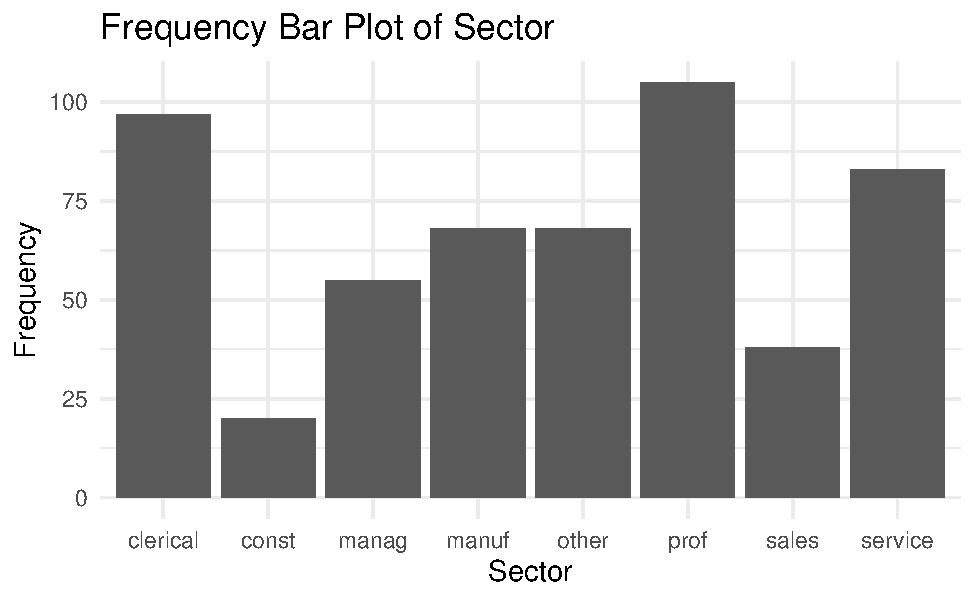
\includegraphics[width=0.5\linewidth]{03-EDA-categorical_files/figure-latex/unnamed-chunk-3-1} \end{center}

\begin{enumerate}
\def\labelenumi{\arabic{enumi}.}
\setcounter{enumi}{3}
\tightlist
\item
  Which features in the relative frequency bar plot are the same as the frequency bar plot? Which are different?
\end{enumerate}

\vspace{1in}

\newpage

\hypertarget{displaying-two-categorical-variables}{%
\subsubsection*{Displaying two categorical variables}\label{displaying-two-categorical-variables}}
\addcontentsline{toc}{subsubsection}{Displaying two categorical variables}

To examine the differences in level of myopia for the level of light, we would create a segmented bar plot of \texttt{Light} segmented by \texttt{Sight}. To create the segmented bar plot enter the variable name, \texttt{Light} (explanatory variable) for xx and the variable name, \texttt{Sight} (response variable) for yy in the \texttt{R} script file in line 28. Highlight and run lines 27--33.

\begin{Shaded}
\begin{Highlighting}[]
\NormalTok{myopia }\OperatorTok\StringTok{ }\CommentTok{# Data set piped into...}
\KeywordTok{ggplot}\NormalTok{(}\KeywordTok{aes}\NormalTok{(}\DataTypeTok{x =}\NormalTok{ xx, }\DataTypeTok{fill =}\NormalTok{ yy)) }\OperatorTok{+}\StringTok{   }\CommentTok{# This specifies the variables}
\StringTok{  }\KeywordTok{geom_bar}\NormalTok{(}\DataTypeTok{stat =} \StringTok{"count"}\NormalTok{, }\DataTypeTok{position =} \StringTok{"fill"}\NormalTok{) }\OperatorTok{+}\StringTok{  }\CommentTok{# Tell it to make a stacked bar plot}
\StringTok{  }\KeywordTok{labs}\NormalTok{(}\DataTypeTok{title =} \StringTok{"Segmented Bar Plot of Night Light Use by Level of Myopia"}\NormalTok{,  }
       \CommentTok{# Make sure to title your plot }
       \DataTypeTok{x =} \StringTok{"Level of Light"}\NormalTok{,   }\CommentTok{# Label the x axis}
       \DataTypeTok{y =} \StringTok{""}\NormalTok{) }\OperatorTok{+}\StringTok{  }\CommentTok{# Remove y axis label}
\StringTok{    }\KeywordTok{scale_fill_grey}\NormalTok{()  }\CommentTok{# Make figure black and white}
\end{Highlighting}
\end{Shaded}

\begin{enumerate}
\def\labelenumi{\arabic{enumi}.}
\setcounter{enumi}{4}
\tightlist
\item
  Sketch the segmented bar plot created here. Be sure to label the axes.
\end{enumerate}

\vspace{1.5in}

\begin{enumerate}
\def\labelenumi{\arabic{enumi}.}
\setcounter{enumi}{5}
\tightlist
\item
  From the segmented bar plot, estimate the proportion of no myopia for those that used a Nightlight.
\end{enumerate}

\vspace{0.5in}

\begin{enumerate}
\def\labelenumi{\arabic{enumi}.}
\setcounter{enumi}{6}
\tightlist
\item
  Which level of light has the highest proportion of \texttt{No\ Myopia}?
\end{enumerate}

\vspace{0.5in}

\hypertarget{take-home-messages}{%
\subsection{Take-home messages}\label{take-home-messages}}

\begin{enumerate}
\def\labelenumi{\arabic{enumi}.}
\item
  Bar charts can be used to graphically display a single categorical variable either as counts or proportions. Segmented bar charts and mosaic plots are used to display two categorical variables.
\item
  Segmented bar charts always have a scale from 0 - 100\%. The bars represent the outcomes of the explanatory variable. Each bar is segmented by the response variable. If the heights of each segment are the same for each bar there is no association between variables.
\item
  Mosaic plots are similar to segmented bar charts but the widths of the bars also show the number of observations within each outcome.
\item
  Conditional probabilities are calculated dependent on a second variable. In the probability notation, the variable following \texttt{\textbar{}} is the variable on which we are conditioning. The denominator used to calculate the probability will be the total for the variable on which we are conditioning.
\end{enumerate}

\newpage

\hypertarget{additional-notes}{%
\subsection{Additional notes}\label{additional-notes}}

Use this space to summarize your thoughts and take additional notes on this week's activity and material covered.

\hypertarget{exploring-quantitative-data}{%
\chapter{Exploring Quantitative Data}\label{exploring-quantitative-data}}

\hypertarget{reading-guide-quantitative-data}{%
\section{Reading Guide: Quantitative Data}\label{reading-guide-quantitative-data}}

\hypertarget{section-2.3-exploring-quantitative-data}{%
\subsection*{Section 2.3 (Exploring quantitative data)}\label{section-2.3-exploring-quantitative-data}}
\addcontentsline{toc}{subsection}{Section 2.3 (Exploring quantitative data)}

\textbf{Videos}

\begin{itemize}
\tightlist
\item
  2.3
\end{itemize}

\setstretch{1.25}

\hypertarget{types-of-plots}{%
\subsection*{Types of plots}\label{types-of-plots}}
\addcontentsline{toc}{subsection}{Types of plots}

Scatterplot:
\rgs

Dot plot:
\rgs

Histogram:
\rgs

Density plot:
\rgs

Box plot:
\rgs

\hypertarget{vocabulary}{%
\subsubsection*{Vocabulary}\label{vocabulary}}
\addcontentsline{toc}{subsubsection}{Vocabulary}

Four characteristics of a scatterplot:

\rgi Form:
\rgs

\rgi Strength:
\rgs

\rgi Direction:
\rgs

\rgi Unusual observations or outliers:
\rgs

Data density:
\rgs

Tail:
\rgs

Skew:
\rgs

Symmetric:
\rgs

Modality:
\rgs

Distribution (of a variable):
\rgs

\rgi Four characteristics of the distribution of 1 quantitative variable:

\rgi Center:
\rgs

\rgi Variability:
\rgs

\rgi Shape:
\rgs

\rgi Outliers:
\rgs

Point estimate:
\rgs

Deviation:
\rgs

Five number summary:
\rgs

\(X^{th}\) percentile:
\rgs

\rgi E.g., if the value 6 is 10th percentile, then 10\% of the data have values 6 or below.

Interquartile range (IQR):
\rgs

Robust statistics:
\rgs

\hypertarget{notes}{%
\subsubsection*{Notes}\label{notes}}
\addcontentsline{toc}{subsubsection}{Notes}

What type of plot(s) are appropriate for displaying one quantitative variable?
\rgs

What type of plot(s) are appropriate for displaying two quantitative variables?
\rgs

What type of plot(s) are appropriate for displaying one quantitative variable and one categorical variable?
\rgs

What are the two ways to measure the `center' of a distribution? Which one is considered robust to skew/outliers?
\rgs

What are the three ways to measure the `variability' of a distribution? Which one is considered robust to skew/outliers?
\rgs

How are variance and standard deviation related?
\rgs

Fill in the following table with the appropriate notation.

\begin{center}
\begin{tabular}{|l|p{2in}|p{2in}|} \hline
Summary Measure & Parameter & Statistic \\ \hline
Mean & & \\ 
& & \\ \hline
Variance & & \\ 
& & \\ \hline
Standard deviation & & \\ 
& & \\ \hline
\end{tabular}
\end{center}

How are outliers denoted on a box plot? How can you mathematically determine if a data set has outliers?
\rgs
\rgs

\hypertarget{section-2.4-r-exploratory-data-analysis-and-section-2.5-chapter-2-review}{%
\subsection*{\texorpdfstring{Section 2.4 (\texttt{R}: Exploratory data analysis) and Section 2.5 (Chapter 2 review)}{Section 2.4 (R: Exploratory data analysis) and Section 2.5 (Chapter 2 review)}}\label{section-2.4-r-exploratory-data-analysis-and-section-2.5-chapter-2-review}}
\addcontentsline{toc}{subsection}{Section 2.4 (\texttt{R}: Exploratory data analysis) and Section 2.5 (Chapter 2 review)}

Section 2.4 presents four tutorials on analyzing quantitative data in \texttt{R}. We recommend you complete all four.

\hypertarget{notes-1}{%
\subsubsection*{Notes}\label{notes-1}}
\addcontentsline{toc}{subsubsection}{Notes}

Statistics summarize \_\_\_\_\_\_\_\_\_\_\_\_\_ .

Parameters summarize \_\_\_\_\_\_\_\_\_\_\_\_\_.

\newpage

Fill in the following table with the appropriate notation for each summary measure.

\begin{center}
\begin{tabular}{|l|p{2in}|p{2in}|}\hline
Summary measure & Statistic & Parameter \\ \hline
Sample size & & \\ 
& & \\ \hline
Proportion & & \\ 
(used to summarize & & \\ 
one categorical variable) & & \\ \hline
Mean & & \\ 
(used to summarize & & \\ 
one quantitative variable)& & \\ \hline
Correlation & & \\ 
(used to summarize & & \\ 
two quantitative variables)& & \\ \hline
Regression line slope & & \\ 
(used to summarize & & \\ 
two quantitative variables)& & \\ \hline
\end{tabular}
\end{center}

\rgs

Look at the table of vocabulary terms. If there are any you do not know, be sure to review the appropriate section of your text.

\hypertarget{data-visualization-summary}{%
\subsubsection*{Data visualization summary}\label{data-visualization-summary}}
\addcontentsline{toc}{subsubsection}{Data visualization summary}

Fill in the following table to help associate type of plot for each of several scenarios.

\begin{center}
\begin{tabular}{|l|p{3in}|} \hline
 & Appropriate plot(s) \\ \hline
One categorical variable & \\
(categorical response, no explanatory) & \\ \hline
One quantitative variable  & \\
(quantitative response, no explanatory) & \\ \hline
Two categorical variables  & \\
(categorical response, categorical explanatory) & \\ \hline
One of each  & \\
(quantitative response, categorical explanatory) & \\ \hline
Two quantitative variables  & \\
(quantitative response, quantitative explanatory) & \\ \hline
\end{tabular}
\end{center}

\rgs

\newpage

Decision tree for determining an appropriate plot given a number of variables and their types from Chapter 2 review:

\begin{center}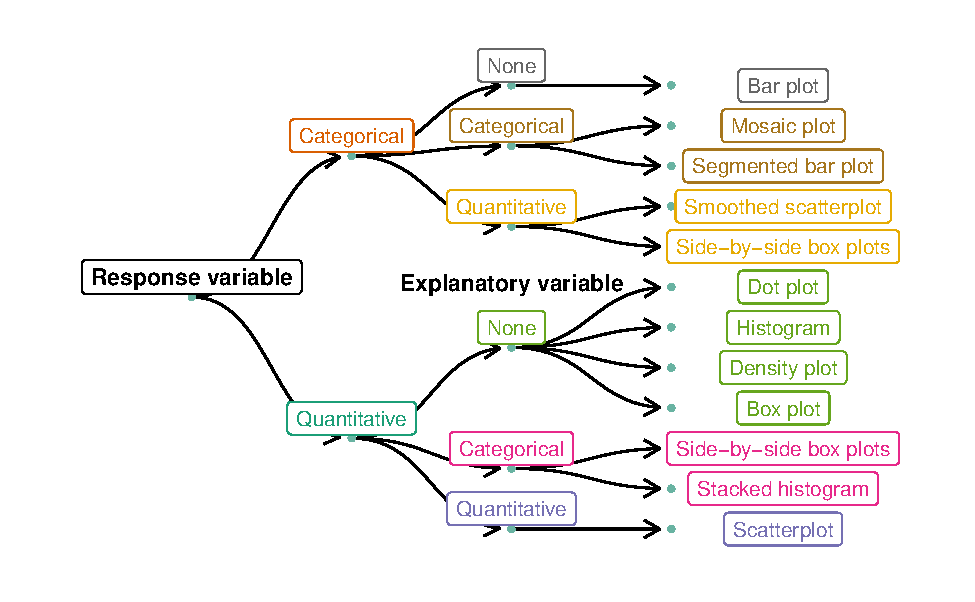
\includegraphics[width=0.7\linewidth]{04-EDA-quantitative_files/figure-latex/decision-tree-plots-1} \end{center}

\newpage

\hypertarget{activity-imdb-movie-reviews}{%
\section{Activity: IMDb Movie Reviews}\label{activity-imdb-movie-reviews}}

\setstretch{1}

\hypertarget{learning-objectives}{%
\subsection{Learning objectives}\label{learning-objectives}}

\begin{itemize}
\item
  Identify and create appropriate summary statistics and plots given a data set or research question for quantitative data.
\item
  Interpret the following summary statistics in context:
  median, lower quartile, upper quartile,
  standard deviation, inter-quartile range.
\item
  Given a plot or set of plots, describe and compare the distribution(s) of a single quantitative variable (center, variability, shape, outliers).
\end{itemize}

\hypertarget{terminology-review}{%
\subsection{Terminology review}\label{terminology-review}}

In this week's activity, we will review summary measures and plots for quantitative variables. Some terms covered in this activity are:

\begin{itemize}
\item
  Two measures of center: mean, median
\item
  Two measures of spread (variability): standard deviation, inter-quartile range (IQR)
\item
  Types of graphs: box plots, dot plots, histograms
\end{itemize}

To review these concepts, see Section 2.3 in the textbook.

\hypertarget{movies-released-in-2016}{%
\subsection{Movies released in 2016}\label{movies-released-in-2016}}

A data set was collected on movies released in 2016. Here is a list of some of the variables collected on these movies.

\begin{longtable}[]{@{}ll@{}}
\toprule
\begin{minipage}[b]{0.22\columnwidth}\raggedright
\textbf{Variable}\strut
\end{minipage} & \begin{minipage}[b]{0.72\columnwidth}\raggedright
\textbf{Description}\strut
\end{minipage}\tabularnewline
\midrule
\endhead
\begin{minipage}[t]{0.22\columnwidth}\raggedright
\texttt{budget\_mil}\strut
\end{minipage} & \begin{minipage}[t]{0.72\columnwidth}\raggedright
Amount of money (in US \$ millions) budgeted for the production of the movie\strut
\end{minipage}\tabularnewline
\begin{minipage}[t]{0.22\columnwidth}\raggedright
\texttt{revenue\_mil}\strut
\end{minipage} & \begin{minipage}[t]{0.72\columnwidth}\raggedright
Amount of money (in US \$ millions) the movie made after release\strut
\end{minipage}\tabularnewline
\begin{minipage}[t]{0.22\columnwidth}\raggedright
\texttt{duration}\strut
\end{minipage} & \begin{minipage}[t]{0.72\columnwidth}\raggedright
Length of the movie (in minutes)\strut
\end{minipage}\tabularnewline
\begin{minipage}[t]{0.22\columnwidth}\raggedright
\texttt{content\_rating}\strut
\end{minipage} & \begin{minipage}[t]{0.72\columnwidth}\raggedright
Rating of the movie (\texttt{G}, \texttt{PG}, \texttt{PG-13}, \texttt{R}, \texttt{Not\ Rated})\strut
\end{minipage}\tabularnewline
\begin{minipage}[t]{0.22\columnwidth}\raggedright
\texttt{imdb\_score}\strut
\end{minipage} & \begin{minipage}[t]{0.72\columnwidth}\raggedright
IMDb user rating score from 1 to 10\strut
\end{minipage}\tabularnewline
\begin{minipage}[t]{0.22\columnwidth}\raggedright
\texttt{genres}\strut
\end{minipage} & \begin{minipage}[t]{0.72\columnwidth}\raggedright
Categories the movie falls into (e.g., Action, Drama, etc.)\strut
\end{minipage}\tabularnewline
\begin{minipage}[t]{0.22\columnwidth}\raggedright
\texttt{movie\_facebook\_likes}\strut
\end{minipage} & \begin{minipage}[t]{0.72\columnwidth}\raggedright
Number of likes a movie receives on Facebook\strut
\end{minipage}\tabularnewline
\bottomrule
\end{longtable}

\hypertarget{vocabulary-review.-complete-q1q3-before-class.}{%
\subsubsection*{Vocabulary review. Complete Q1--Q3 before class.}\label{vocabulary-review.-complete-q1q3-before-class.}}
\addcontentsline{toc}{subsubsection}{Vocabulary review. Complete Q1--Q3 before class.}

\begin{enumerate}
\def\labelenumi{\arabic{enumi}.}
\tightlist
\item
  What are the observational units in this data set?
\end{enumerate}

\vspace{0.1in}

\begin{enumerate}
\def\labelenumi{\arabic{enumi}.}
\setcounter{enumi}{1}
\tightlist
\item
  Which of the above listed variables are categorical?
\end{enumerate}

\vspace{.5in}

\begin{enumerate}
\def\labelenumi{\arabic{enumi}.}
\setcounter{enumi}{2}
\tightlist
\item
  Which of the above listed variables are quantitative?
\end{enumerate}

\vspace{.5in}

\hypertarget{summarizing-a-single-quantitative-variable}{%
\subsubsection*{Summarizing a single quantitative variable}\label{summarizing-a-single-quantitative-variable}}
\addcontentsline{toc}{subsubsection}{Summarizing a single quantitative variable}

The \texttt{favstats} function from the \texttt{mosaic} package gives the summary statistics for a quantitative variable. Here we have the summary statistics for the variable \texttt{imdb\_score}.

\begin{Shaded}
\begin{Highlighting}[]
\NormalTok{movies <-}\StringTok{ }\KeywordTok{read.csv}\NormalTok{(}\StringTok{"data/Movies2016.csv"}\NormalTok{) }\CommentTok{# Read in data set}
\NormalTok{movies }\OperatorTok\StringTok{ }\CommentTok{# Data set piped into...}
\StringTok{  }\KeywordTok{summarise}\NormalTok{(}\KeywordTok{favstats}\NormalTok{(imdb_score)) }\CommentTok{# Apply favstats function to imdb_score}
\end{Highlighting}
\end{Shaded}

\begin{verbatim}
#>   min   Q1 median  Q3 max     mean       sd  n missing
#> 1 3.4 5.65    6.4 7.1 8.2 6.309783 1.086689 92       0
\end{verbatim}

\begin{enumerate}
\def\labelenumi{\arabic{enumi}.}
\setcounter{enumi}{3}
\tightlist
\item
  Give the values for the two measures of center.
\end{enumerate}

\vspace{0.5in}

\begin{enumerate}
\def\labelenumi{\arabic{enumi}.}
\setcounter{enumi}{4}
\tightlist
\item
  Calculate the interquartile range (IQR = Q3 \(-\) Q1).
\end{enumerate}

\vspace{0.5in}

\begin{enumerate}
\def\labelenumi{\arabic{enumi}.}
\setcounter{enumi}{5}
\tightlist
\item
  Report the value of the standard deviation and interpret this value in context of the problem.
  \vspace{1in}
\end{enumerate}

\hypertarget{displaying-a-single-quantitative-variable}{%
\subsubsection*{Displaying a single quantitative variable}\label{displaying-a-single-quantitative-variable}}
\addcontentsline{toc}{subsubsection}{Displaying a single quantitative variable}

\begin{enumerate}
\def\labelenumi{\arabic{enumi}.}
\setcounter{enumi}{6}
\tightlist
\item
  What are the three types of plots used to plot a single quantitative variable?
\end{enumerate}

\vspace{1in}

To create a histogram of the IMDb scores, enter the variable name, \texttt{imdb\_score} in the provided \texttt{R} script file for xx at line 12, highlight and run lines 1--16. Visually, this shows us the range of IMDb scores for Movies released in 2016.

Notice that the \textbf{bin width} is 0.5. For example the first bin consists of the number of movies in the data set with an IMDb score of 3.25 to 3.75. It is important to note that a movie with a IMDb score on the boundary of a bin will fall into the bin above it; for example, 4.76 would be counted in the bin 4.75--5.25.

\begin{Shaded}
\begin{Highlighting}[]
\NormalTok{movies }\OperatorTok\StringTok{ }\CommentTok{# Data set piped into...}
\KeywordTok{ggplot}\NormalTok{(}\KeywordTok{aes}\NormalTok{(}\DataTypeTok{x =}\NormalTok{ xx)) }\OperatorTok{+}\StringTok{   }\CommentTok{# Name variable to plot}
\StringTok{  }\KeywordTok{geom_histogram}\NormalTok{(}\DataTypeTok{binwidth =} \FloatTok{0.5}\NormalTok{) }\OperatorTok{+}\StringTok{  }\CommentTok{# Create histogram with specified binwidth}
\StringTok{  }\KeywordTok{labs}\NormalTok{(}\DataTypeTok{title =} \StringTok{"Histogram of IMDb Score of Movies in 2016"}\NormalTok{, }\CommentTok{# Title for plot}
       \DataTypeTok{x =} \StringTok{"IMDb Score"}\NormalTok{, }\CommentTok{# Label for x axis}
       \DataTypeTok{y =} \StringTok{"Frequency"}\NormalTok{) }\CommentTok{# Label for y axis}
\end{Highlighting}
\end{Shaded}

\newpage

\begin{enumerate}
\def\labelenumi{\arabic{enumi}.}
\setcounter{enumi}{7}
\tightlist
\item
  Sketch the histogram created here.
\end{enumerate}

\vspace{1in}

\begin{enumerate}
\def\labelenumi{\arabic{enumi}.}
\setcounter{enumi}{8}
\tightlist
\item
  Which range of IMDb scores have the highest frequency?
\end{enumerate}

\vspace{0.3in}

\begin{enumerate}
\def\labelenumi{\arabic{enumi}.}
\setcounter{enumi}{9}
\tightlist
\item
  What is the shape of the distribution of IMDb scores?
\end{enumerate}

\vspace{0.3in}

\begin{enumerate}
\def\labelenumi{\arabic{enumi}.}
\setcounter{enumi}{10}
\tightlist
\item
  Which five summary statistics are used in creating a box plot? \emph{Hint}: Together they are called the \textbf{five-number summary} of the variable.
\end{enumerate}

\vspace{0.3in}

\begin{enumerate}
\def\labelenumi{\arabic{enumi}.}
\setcounter{enumi}{11}
\item
  Using the code below, we see that the three smallest IMDb scores in the data set are 3.4, 3.5, and 3.7 and the three largest IMDb scores are 8.0, 8.1, and 8.2:

\begin{Shaded}
\begin{Highlighting}[]
\NormalTok{movies }\OperatorTok\StringTok{ }\CommentTok{# Data set pipes into...}
\StringTok{  }\KeywordTok{select}\NormalTok{(imdb_score) }\OperatorTok\StringTok{ }\CommentTok{# Select imdb_score variable}
\StringTok{  }\KeywordTok{slice_min}\NormalTok{(imdb_score, }\DataTypeTok{n =} \DecValTok{3}\NormalTok{)  }\CommentTok{# Show 3 smallest values}
\end{Highlighting}
\end{Shaded}

\begin{verbatim}
#>   imdb_score
#> 1        3.4
#> 2        3.5
#> 3        3.7
\end{verbatim}

\begin{Shaded}
\begin{Highlighting}[]
\NormalTok{movies }\OperatorTok\StringTok{ }\CommentTok{# Data set pipes into...}
\StringTok{  }\KeywordTok{select}\NormalTok{(imdb_score) }\OperatorTok\StringTok{ }\CommentTok{# Select imdb_score variable}
\StringTok{  }\KeywordTok{slice_max}\NormalTok{(imdb_score, }\DataTypeTok{n =} \DecValTok{3}\NormalTok{)  }\CommentTok{# Show 3 largest values}
\end{Highlighting}
\end{Shaded}

\begin{verbatim}
#>   imdb_score
#> 1        8.2
#> 2        8.1
#> 3        8.0
\end{verbatim}

  Using the summary statistics displayed in the \texttt{favstats} output, and the smallest and largest values of the variable to check for outliers, sketch a box plot of IMDb Score. Be sure to label the axis.
\end{enumerate}

\vspace{1.5in}

\newpage

\hypertarget{displaying-a-single-categorical-and-single-quantitative-variable}{%
\subsubsection*{Displaying a single categorical and single quantitative variable}\label{displaying-a-single-categorical-and-single-quantitative-variable}}
\addcontentsline{toc}{subsubsection}{Displaying a single categorical and single quantitative variable}

The box plot of movie budgets (in millions) by content rating is plotted using the code below. Enter the variable \texttt{budget\_mil} for yy and the variable \texttt{content\_rating} for xx at line 31, highlight and run code lines 29--35. This plot helps to compare the budget distribution for different levels of content rating.

\begin{Shaded}
\begin{Highlighting}[]
\NormalTok{movies }\OperatorTok\StringTok{  }\CommentTok{# Data set piped into...}
\StringTok{  }\KeywordTok{filter}\NormalTok{(content_rating }\OperatorTok{!=}\StringTok{ "Not Rated"}\NormalTok{) }\OperatorTok\StringTok{ }\CommentTok{# Remove Not Rated movies}
\StringTok{  }\KeywordTok{ggplot}\NormalTok{(}\KeywordTok{aes}\NormalTok{(}\DataTypeTok{y =}\NormalTok{ yy, }\DataTypeTok{x =}\NormalTok{ xx))}\OperatorTok{+}\StringTok{  }\CommentTok{# Identify variables}
\StringTok{  }\KeywordTok{geom_boxplot}\NormalTok{()}\OperatorTok{+}\StringTok{  }\CommentTok{# Tell it to make a box plot}
\StringTok{  }\KeywordTok{labs}\NormalTok{(}\DataTypeTok{title =} \StringTok{"Side by side box plot of budget by content rating"}\NormalTok{,  }\CommentTok{# Title}
       \DataTypeTok{x =} \StringTok{"Content Rating"}\NormalTok{,    }\CommentTok{# x-axis label}
       \DataTypeTok{y =} \StringTok{"Budget (in Millions)"}\NormalTok{)  }\CommentTok{# y-axis label}
\end{Highlighting}
\end{Shaded}

\begin{enumerate}
\def\labelenumi{\arabic{enumi}.}
\setcounter{enumi}{12}
\tightlist
\item
  Sketch the box plots created from running the \texttt{R} code above.
\end{enumerate}

\vspace{1.5in}

\begin{enumerate}
\def\labelenumi{\arabic{enumi}.}
\setcounter{enumi}{13}
\tightlist
\item
  Answer the following questions about the box plots created.
\end{enumerate}

\begin{enumerate}
\def\labelenumi{\alph{enumi}.}
\item
  Which content rating has the highest center?
  \vspace{0.2in}
\item
  Which content rating has the largest spread?
  \vspace{0.2in}
\item
  Which content rating has the most skewed distribution?
  \vspace{0.2in}
\item
  Fifty percent of movies in 2016 with a PG-13 content rating fall below what value? What is the name of this value?
  \vspace{0.4in}
\item
  What is the value for the third quartile (Q3) for the PG-13 rating? Interpret this value in context.
  \vspace{.8in}
\end{enumerate}

\newpage

\hypertarget{out-of-class-activity}{%
\subsection{Out-of-class activity}\label{out-of-class-activity}}

For a little more practice using RStudio to create graphs of quantitative variables, we will look at some other variables in the \texttt{Movies} data set. Download and open the provided \texttt{R} script file, highlight and run the first 8 lines of code.

To use the \texttt{favstats} function in the \texttt{mosaic} package with two variables, we will enter the variables as a formula, \texttt{response\ \textasciitilde{}\ explanatory}.

\begin{Shaded}
\begin{Highlighting}[]
\NormalTok{movies }\OperatorTok\StringTok{ }\CommentTok{# Data set piped into...}
\StringTok{  }\KeywordTok{summarise}\NormalTok{(}\KeywordTok{favstats}\NormalTok{(imdb_score }\OperatorTok{~}\StringTok{ }\NormalTok{content_rating)) }\CommentTok{# Summary stats of imdb_score by content rating}
\end{Highlighting}
\end{Shaded}

\begin{verbatim}
#>   content_rating min    Q1 median    Q3 max     mean        sd  n missing
#> 1      Not Rated 3.7 4.700    5.7 6.700 7.7 5.700000 2.8284271  2       0
#> 2             PG 3.4 6.150    6.8 7.225 7.8 6.425000 1.2757351 12       0
#> 3          PG-13 4.0 5.800    6.5 7.100 8.2 6.367391 0.9477586 46       0
#> 4              R 3.5 5.375    6.3 7.050 8.1 6.221875 1.1335740 32       0
\end{verbatim}

Using the provided \texttt{R} script file, we will create side-by-side histograms of IMDb scores by movie content rating. Enter the variable name, \texttt{imdb\_score} for yy and \texttt{content\_rating} for xx at line 44, highlight and run lines 39--48.

\begin{Shaded}
\begin{Highlighting}[]
\NormalTok{movies }\OperatorTok\StringTok{  }\CommentTok{# Data set piped into...}
\StringTok{  }\KeywordTok{filter}\NormalTok{(content_rating }\OperatorTok{!=}\StringTok{ "Not Rated"}\NormalTok{) }\OperatorTok\StringTok{ }\CommentTok{# Remove Not Rated movies}
\StringTok{  }\KeywordTok{ggplot}\NormalTok{(}\KeywordTok{aes}\NormalTok{(}\DataTypeTok{y =}\NormalTok{ yy, }\DataTypeTok{x =}\NormalTok{ xx))}\OperatorTok{+}\StringTok{  }\CommentTok{# Identify variables}
\StringTok{  }\KeywordTok{geom_boxplot}\NormalTok{()}\OperatorTok{+}\StringTok{  }\CommentTok{# Tell it to make a box plot}
\StringTok{  }\KeywordTok{labs}\NormalTok{(}\DataTypeTok{title =} \StringTok{"Side by side box plot of budget by content rating"}\NormalTok{,  }\CommentTok{# Title}
       \DataTypeTok{x =} \StringTok{"Content Rating"}\NormalTok{,    }\CommentTok{# x-axis label}
       \DataTypeTok{y =} \StringTok{"Budget (in Millions)"}\NormalTok{)  }\CommentTok{# y-axis label}
\end{Highlighting}
\end{Shaded}

\begin{enumerate}
\def\labelenumi{\arabic{enumi}.}
\tightlist
\item
  Using the provided \texttt{favstats} output and the side-by-side box plots, interpret the value of quartile 1 for the R content rating.
\end{enumerate}

\vspace{1in}

\begin{enumerate}
\def\labelenumi{\arabic{enumi}.}
\setcounter{enumi}{1}
\tightlist
\item
  Which content rating has the highest center?
\end{enumerate}

\vspace{0.2in}

\begin{enumerate}
\def\labelenumi{\arabic{enumi}.}
\setcounter{enumi}{2}
\tightlist
\item
  Which variable is the explanatory variable in the side-by-side box plots? Response variable?
\end{enumerate}

\vspace{0.5in}

\hypertarget{take-home-messages}{%
\subsection{Take-home messages}\label{take-home-messages}}

\begin{enumerate}
\def\labelenumi{\arabic{enumi}.}
\item
  Histograms, box plots, and dot plots can all be used to graphically display quantitative variables. When we have a single categorical variable and a single quantitative variable we will display the data in side-by-side plots.
\item
  The box plot is created using the five number summary: minimum value, quartile 1, median, quartile 3, and maximum value. Values in the data set that are less than \(Q_1 - 1.5 \times IQR\) and greater than \(Q_3 + 1.5\times IQR\) are considering outliers and are graphically represented by a dot outside of the whiskers on the box plot. Whiskers extend to the smallest and largest values in the data set that are \emph{not} considered outliers.
\item
  When comparing distributions of quantitative variables we look at the shape, center, spread, and for outliers. There are two measures of center: mean and median; and two measures of spread: standard deviation and the interquartile range, IQR = Q1 \(-\) Q3.
\item
  The median and IQR are robust measures that are not affected by the presence of outliers or skewness; the mean and standard deviation are not robust and can be greatly affected by skewness and the presence of outliers.
\end{enumerate}

\hypertarget{additional-notes}{%
\subsection{Additional notes}\label{additional-notes}}

Use this space to summarize your thoughts and take additional notes on this week's activity and material covered.

\hypertarget{exploring-multivariable-data}{%
\chapter{Exploring Multivariable Data}\label{exploring-multivariable-data}}

\hypertarget{reading-guide-quantitative-data}{%
\section{Reading Guide: Quantitative Data}\label{reading-guide-quantitative-data}}

\hypertarget{section-3.1-fitting-a-line-residuals-and-correlation}{%
\subsection*{Section 3.1 (Fitting a line, residuals, and correlation)}\label{section-3.1-fitting-a-line-residuals-and-correlation}}
\addcontentsline{toc}{subsection}{Section 3.1 (Fitting a line, residuals, and correlation)}

\setstretch{1}

\textbf{Videos}

\begin{itemize}
\tightlist
\item
  Chapter3
\end{itemize}

\setstretch{1.25}

\hypertarget{reminders-from-section-2.3}{%
\subsubsection*{Reminders from Section 2.3}\label{reminders-from-section-2.3}}
\addcontentsline{toc}{subsubsection}{Reminders from Section 2.3}

Scatterplot: displays two quantitative variables; one dot = two measurements (\(x\), \(y\)) on one observational unit

Four characteristics of a scatterplot:
\setstretch{1}

\begin{itemize}
\tightlist
\item
  \emph{Form}: pattern of the dots plotted. Is the trend generally linear (you can fit a straight line to the data) or non-linear?\\
\item
  \emph{Strength}: how closely do the points follow a trend? Very closely (strong)? No pattern (weak)?\\
\item
  \emph{Direction}: as the \(x\) values increase, do the \(y\)-values tend to increase (positive) or decrease (negative)?\\
\item
  Unusual observations or \emph{outliers}: points that do not fit the overall pattern of the data.
\end{itemize}

\setstretch{1.25}

\hypertarget{vocabulary}{%
\subsubsection*{Vocabulary}\label{vocabulary}}
\addcontentsline{toc}{subsubsection}{Vocabulary}

Residual:
\rgs

\rgi Formula:
\rgs

Residual plot:
\rgs

Correlation:
\rgs

\hypertarget{notes}{%
\subsubsection*{Notes}\label{notes}}
\addcontentsline{toc}{subsubsection}{Notes}

General equation of a linear regression for a \emph{population}: \(y= \beta_0+ \beta_1 x+\epsilon\), where

\rgi \(x\) represents
\rgs

\rgi \(y\) represents
\rgs

\rgi \(\beta_0\) represents
\rgs

\rgi \(\beta_1\) represents
\rgs

\rgi \(\epsilon\) represents
\rgs

General equation of a linear regression model from \emph{sample} data: \(\hat{y}= b_0+ b_1 x\), where

\rgi \(x\) represents
\rgs

\rgi \(\hat{y}\) represents
\rgs

\rgi \(b_0\) represents
\rgs

\rgi \(b_1\) represents
\rgs

Fill in the following table with the appropriate notation for each summary measure.

\begin{center}
\begin{tabular}{|l|p{2in}|p{2in}|} \hline
Summary Measure & Parameter & Statistic \\ \hline
Correlation & & \\ 
& & \\ \hline
Slope & & \\ 
& & \\ \hline
$y$-intercept & & \\ 
& & \\ \hline
\end{tabular}
\end{center}

Fill in the blanks below to define some of the properties of correlation:

\rgi The value of correlation must be between \_\_\_\_\_\_\_\_\_\_\_. (Includes the endpoints of the interval)

\rgi The sign of correlation gives the \_\_\_\_\_\_\_\_\_\_\_\_\_\_ of the linear relationship.

\rgi The magnitude of correlation gives the \_\_\_\_\_\_\_\_\_\_\_\_ of the linear relationship.

True or false: A scatterplot that shows random scatter would be considered non-linear.

True or false: If the correlation between two quantitative variables is equal to zero, then the two variables are not associated.

True or false: To calculate a predicted \(y\)-value from a given \(x\)-value, just look at the scatterplot and estimate the \(y\)-value.

True or false: A positive residual indicates the data point is above the regression line.

\newpage

\hypertarget{example-brushtail-possums}{%
\subsubsection*{Example: Brushtail possums}\label{example-brushtail-possums}}
\addcontentsline{toc}{subsubsection}{Example: Brushtail possums}

\begin{enumerate}
\def\labelenumi{\arabic{enumi}.}
\item
  What are the observational units?\\
  \rgs
\item
  Look at the scatterplot in Figure 3.5.
\end{enumerate}

\rgi a) What is the explanatory variable? The response variable? What type is each?
\rgs

\rgi b) What is the form of the scatterplot?
\rgs

\rgi c) What is the direction of the scatterplot?
\rgs

\rgi d) What is the strength of the scatterplot?
\rgs

\rgi e) Are there any outliers on the scatterplot?
\rgs

\begin{enumerate}
\def\labelenumi{\arabic{enumi}.}
\setcounter{enumi}{2}
\item
  Write the equation of the regression line, in context (do not use \(x\) and \(y\), use variable names instead).
  \rgs
\item
  Calculate the predicted head length for a possum with a 76.0 cm total length.
  \rgs
\item
  One of the possums in the data set has a total length of 76.0 cm and a head length of 85.1 cm. Calculate the residual for this possum. Does this possum lie above or below the regression line?
  \rgs
\end{enumerate}

\hypertarget{section-3.2-least-squares-regression}{%
\subsection*{Section 3.2 (Least squares regression)}\label{section-3.2-least-squares-regression}}
\addcontentsline{toc}{subsection}{Section 3.2 (Least squares regression)}

\setstretch{1}

You may skip the special topic Sections 3.2.3.1 and 3.2.6.

\textbf{Videos}

\begin{itemize}
\tightlist
\item
  Chapter3
\end{itemize}

\setstretch{1.25}

\hypertarget{vocabulary-1}{%
\subsubsection*{Vocabulary}\label{vocabulary-1}}
\addcontentsline{toc}{subsubsection}{Vocabulary}

Least squares criterion:
\rgs

Least squares line:
\rgs

\texttt{lm()} \texttt{R} function:
\rgi \texttt{name\_of\_model\ \textless{}-\ lm(response\ \textasciitilde{}\ explanatory,\ data\ =\ data\_set\_name)}

\rgs

slope:
\rgs

\(y\)-intercept:\\
\rgs

Extrapolation:

\rgi Assumes the pattern seen in the data extends beyond the data collected!

Coefficient of determination:

\rgi \(s_y^2\) (or SST) represents
\rgs

\rgi \(s_{RES}^2\) (or SSE) represents
\rgs

\hypertarget{notes-1}{%
\subsubsection*{Notes}\label{notes-1}}
\addcontentsline{toc}{subsubsection}{Notes}

Two methods for determining the best line:

\rgi 1.
\rgs

\rgi 2.
\rgs

Notation for the coefficient of determination:
\rgs

Formulas for calculating the coefficient of determination:
\rgs

True or false: A correlation between two quantitative variables implies a causal relationship exists between the variables.

True or false: The slope of the line tells us how much to expect the \(y\) variable to increase or decrease when the \(x\) variable increases by 1 unit.

True or false: The coefficient of determination is just the square of the correlation.

\hypertarget{example-elmhurst-college}{%
\subsubsection*{Example: Elmhurst College}\label{example-elmhurst-college}}
\addcontentsline{toc}{subsubsection}{Example: Elmhurst College}

\begin{enumerate}
\def\labelenumi{\arabic{enumi}.}
\item
  What are the observational units?\\
  \rgs
\item
  Look at the scatterplot in Figure 3.13.
\end{enumerate}

\rgi a) What is the explanatory variable? The response variable?\\
\rgs

\rgi b) What is the form of the scatterplot?\\
\rgs

\rgi c) What is the direction of the scatterplot?
\rgs

\rgi d) What is the strength of the scatterplot?
\rgs

\rgi e) Are there any outliers on the scatterplot?\\
\rgs

\begin{enumerate}
\def\labelenumi{\arabic{enumi}.}
\setcounter{enumi}{2}
\item
  Write the equation of the regression line, in context (do not use \(x\) and \(y\), use variable names instead).
  \rgs
\item
  Interpret the slope of the line, in the context of the problem. Remember that both family income and gift aid from the university are measured in \$1000s.
  \rgs
  \rgs
\item
  Interpret the \(y\)-intercept of the line, in the context of the problem. Remember that both family income and gift aid from the university are measured in \$1000s.
  \rgs
  \rgs
\item
  Is your interpretation in question 5 an example of extrapolation?
  \rgs
\item
  Give and interpret, in context, the value of the coefficient of determination.
  \rgs
  \rgs
\end{enumerate}

\hypertarget{section-3.3-outliers-in-linear-regression}{%
\subsection*{Section 3.3 (Outliers in linear regression)}\label{section-3.3-outliers-in-linear-regression}}
\addcontentsline{toc}{subsection}{Section 3.3 (Outliers in linear regression)}

\setstretch{1}

\textbf{Videos}

\begin{itemize}
\tightlist
\item
  Chapter3
\end{itemize}

\setstretch{1.25}

\hypertarget{vocabulary-2}{%
\subsubsection*{Vocabulary}\label{vocabulary-2}}
\addcontentsline{toc}{subsubsection}{Vocabulary}

Outlier:
\rgs

Leverage:
\rgs

Influential:
\rgs

\hypertarget{notes-2}{%
\subsubsection*{Notes}\label{notes-2}}
\addcontentsline{toc}{subsubsection}{Notes}

Investigate, but do not remove, outliers. Unless you find there was an actual error in the data collection, ignoring outliers can make models poor predictors!

True or false: All high leverage outliers are influential.

True or false: An outlier is considered high leverage if it is extreme in its \(x\)-value.

\hypertarget{section-3.4-r-correlation-and-regression-and-section-3.5-chapter-3-review}{%
\subsection*{Section 3.4 (R: Correlation and regression) and Section 3.5 (Chapter 3 review)}\label{section-3.4-r-correlation-and-regression-and-section-3.5-chapter-3-review}}
\addcontentsline{toc}{subsection}{Section 3.4 (R: Correlation and regression) and Section 3.5 (Chapter 3 review)}

\setstretch{1}

\textbf{Videos}

\begin{itemize}
\tightlist
\item
  Chapter3
\end{itemize}

\setstretch{1.25}

Section 3.4 presents five tutorials on analyzing two quantitative variables in \texttt{R}. We recommend you complete all five.

\hypertarget{notes-3}{%
\subsubsection*{Notes}\label{notes-3}}
\addcontentsline{toc}{subsubsection}{Notes}

Statistics summarize
\rgs

Parameters summarize
\rgs

What are the two ways to calculate the coefficient of determination?
\rgs

What is the formula for calculating a residual?
\rgs

Determine whether each of the following statements about the correlation coefficient are true or false:

\begin{enumerate}
\def\labelenumi{\arabic{enumi}.}
\item
  The correlation coefficient must be a positive number.
\item
  Stronger linear relationships are indicated by correlation coefficients far from 0.
\item
  The correlation coefficient is a robust statistic.
\item
  When two variables are highly correlated, that indicates a causal relationship exists between the variables.
\item
  The sign of the correlation coefficient will be the same as the sign of the regression line slope, though the values are typically different.
\end{enumerate}

Fill in the blanks to correctly interpret:

\begin{itemize}
\tightlist
\item
  Slope:
\end{itemize}

\begin{verbatim}
For every ____________________________, we expect _________________ to increase (if slope is _____________) or decrease (if slope is ____________) by the absolute value of the _________.
\end{verbatim}

\begin{itemize}
\item
  \(y\)-intercept:

  If \_\_\_\_\_\_\_\_\_\_\_\_\_\_\_, we predict the \_\_\_\_\_\_\_\_\_\_\_\_\_\_\_\_\_\_\_\_\_\_\_\_\_\_ to equal \_\_\_\_\_\_\_\_\_\_.
\end{itemize}

Look at the table of vocabulary terms. If there are any you do not know, be sure to review the appropriate section of your text.

\newpage

\hypertarget{section-4.1-gapminder-world}{%
\subsection*{Section 4.1 (Gapminder world)}\label{section-4.1-gapminder-world}}
\addcontentsline{toc}{subsection}{Section 4.1 (Gapminder world)}

\setstretch{1}

\textbf{Videos}

\begin{itemize}
\tightlist
\item
  Chapter4
\end{itemize}

\setstretch{1.25}

\hypertarget{reminder-from-section-3.1}{%
\subsubsection*{Reminder from Section 3.1}\label{reminder-from-section-3.1}}
\addcontentsline{toc}{subsubsection}{Reminder from Section 3.1}

Use color and a legend to add a third variable to a scatterplot. E.g., Color the dots to represent different levels of a categorical variable or shading to represent different values of a quantitative variable.

\hypertarget{vocabulary-3}{%
\subsubsection*{Vocabulary}\label{vocabulary-3}}
\addcontentsline{toc}{subsubsection}{Vocabulary}

Interaction:
\rgs

Aesthetic:
\rgs

\hypertarget{notes-4}{%
\subsubsection*{Notes}\label{notes-4}}
\addcontentsline{toc}{subsubsection}{Notes}

If the response and one predictor are quantitative and the other predictor categorical, we fit a regression line for each level of the categorical predictor.

\begin{itemize}
\item
  Parallel slopes would indicate that that the two predictors \_\_\_\_\_\_\_\_\_\_\_\_\_\_\_\_\_\_\_ in explaining the response.
\item
  Non-parallel slopes would indicate that the two predictors \_\_\_\_\_\_\_\_\_\_\_\_\_\_\_\_\_\_\_ in explaining the response.
\end{itemize}

True or false: Scatterplots can only display two variables at a time.

\hypertarget{section-4.2-simpsons-paradox-revisited}{%
\subsection*{Section 4.2 (Simpson's Paradox, revisited)}\label{section-4.2-simpsons-paradox-revisited}}
\addcontentsline{toc}{subsection}{Section 4.2 (Simpson's Paradox, revisited)}

\setstretch{1}

\textbf{Videos}

\begin{itemize}
\tightlist
\item
  Chapter4
\end{itemize}

\setstretch{1.25}

\hypertarget{reminder-from-section-2.1}{%
\subsubsection*{Reminder from Section 2.1}\label{reminder-from-section-2.1}}
\addcontentsline{toc}{subsubsection}{Reminder from Section 2.1}

Simpson's Paradox: when the relationship between the explanatory and response variable is reversed when looking at the relationship within different levels of a confounding variable.

\hypertarget{notes-5}{%
\subsubsection*{Notes}\label{notes-5}}
\addcontentsline{toc}{subsubsection}{Notes}

True or false: Simpson's Paradox can only occur when the explanatory, response, and confounding variables are all categorical.

\newpage

\hypertarget{example-sat-scores}{%
\subsubsection*{Example: SAT scores}\label{example-sat-scores}}
\addcontentsline{toc}{subsubsection}{Example: SAT scores}

\begin{enumerate}
\def\labelenumi{\arabic{enumi}.}
\item
  What are the observational units?\\
  \rgs
\item
  Look at the scatterplot in Figure 4.5.
\end{enumerate}

\rgi a) What is the explanatory variable? The response variable?
\rgs

\rgi b) What is the form of the scatterplot?
\rgs

\rgi c) What is the direction of the scatterplot?
\rgs

\rgi d) What is the strength of the scatterplot?
\rgs

\rgi e) Are there any outliers on the scatterplot?
\rgs

\begin{enumerate}
\def\labelenumi{\arabic{enumi}.}
\setcounter{enumi}{2}
\item
  What would need to be done to the study design in order to eliminate the confounding variable: percent of eligible students taking the SAT?
  \rgs
\item
  What features of the scatterplots in Figure 4.6 demonstrate that the percent of eligible students taking the SAT is a confounding variable?
  \rgs
\item
  How does Figure 4.7 demonstrate Simpson's Paradox?
  \rgs
\end{enumerate}

\hypertarget{section-4.4-chapter-4-review}{%
\subsection*{Section 4.4 (Chapter 4 review)}\label{section-4.4-chapter-4-review}}
\addcontentsline{toc}{subsection}{Section 4.4 (Chapter 4 review)}

\setstretch{1}

Section 4.3 discusses multiple regression and presents five tutorials on analyzing multiple variables in \texttt{R}. This section is a special topic, meaning you are not required to read or complete these tutorials.

\textbf{Videos}

\begin{itemize}
\tightlist
\item
  Chapter4
\end{itemize}

\setstretch{1.25}

\hypertarget{notes-6}{%
\subsubsection*{Notes}\label{notes-6}}
\addcontentsline{toc}{subsubsection}{Notes}

To determine if the relationship between two quantitative variables differs across levels of a categorical variable, you should compare
\rgs

Simpson's Paradox:

\newpage

\hypertarget{activity-movie-profits}{%
\section{Activity: Movie Profits}\label{activity-movie-profits}}

\setstretch{1}

\hypertarget{learning-objectives}{%
\subsection{Learning objectives}\label{learning-objectives}}

\begin{itemize}
\item
  Identify and create appropriate summary statistics and plots
  given a data set with two quantitative variables.
\item
  Use scatterplots to assess the relationship between two quantitative variables.
\item
  Find the estimated line of regression using summary statistics and \texttt{R} linear model (\texttt{lm()}) output.
\item
  Interpret the slope coefficient in context of the problem.
\item
  Calculated and interpret \(R^2\), the coefficient of determination, in context of the problem.
\item
  Find the correlation coefficient from \texttt{R} output or from \(R^2\) and the sign of the slope.
\end{itemize}

\hypertarget{terminology-review}{%
\subsection{Terminology review}\label{terminology-review}}

In this week's activity, we will review summary measures and plots for two quantitative variables. Some terms covered in this activity are:

\begin{itemize}
\item
  Scatterplot
\item
  Correlation (\(r\) or \(R\))
\item
  Coefficient of determination (\(r\)-squared or \(R^2\))
\item
  Least-squares line of regression
\item
  Slope and \(y\)-intercept
\item
  Residuals
\end{itemize}

To review these concepts, see Chapter 3 in the textbook.

\hypertarget{movies-released-in-2016}{%
\subsection{Movies released in 2016}\label{movies-released-in-2016}}

We will revisit the data set used last week collected on Movies released in 2016. Here is a reminder of the variables collected on these movies.

\begin{longtable}[]{@{}ll@{}}
\toprule
\begin{minipage}[b]{0.22\columnwidth}\raggedright
\textbf{Variable}\strut
\end{minipage} & \begin{minipage}[b]{0.72\columnwidth}\raggedright
\textbf{Description}\strut
\end{minipage}\tabularnewline
\midrule
\endhead
\begin{minipage}[t]{0.22\columnwidth}\raggedright
\texttt{budget\_mil}\strut
\end{minipage} & \begin{minipage}[t]{0.72\columnwidth}\raggedright
Amount of money (in US \$ millions) budgeted for the production of the movie\strut
\end{minipage}\tabularnewline
\begin{minipage}[t]{0.22\columnwidth}\raggedright
\texttt{revenue\_mil}\strut
\end{minipage} & \begin{minipage}[t]{0.72\columnwidth}\raggedright
Amount of money (in US \$ millions) the movie made after release\strut
\end{minipage}\tabularnewline
\begin{minipage}[t]{0.22\columnwidth}\raggedright
\texttt{duration}\strut
\end{minipage} & \begin{minipage}[t]{0.72\columnwidth}\raggedright
Length of the movie (in minutes)\strut
\end{minipage}\tabularnewline
\begin{minipage}[t]{0.22\columnwidth}\raggedright
\texttt{content\_rating}\strut
\end{minipage} & \begin{minipage}[t]{0.72\columnwidth}\raggedright
Rating of the movie (\texttt{G}, \texttt{PG}, \texttt{PG-13}, \texttt{R}, \texttt{Not\ Rated})\strut
\end{minipage}\tabularnewline
\begin{minipage}[t]{0.22\columnwidth}\raggedright
\texttt{imdb\_score}\strut
\end{minipage} & \begin{minipage}[t]{0.72\columnwidth}\raggedright
IMDb user rating score from 1 to 10\strut
\end{minipage}\tabularnewline
\begin{minipage}[t]{0.22\columnwidth}\raggedright
\texttt{genres}\strut
\end{minipage} & \begin{minipage}[t]{0.72\columnwidth}\raggedright
Categories the movie falls into (e.g., Action, Drama, etc.)\strut
\end{minipage}\tabularnewline
\begin{minipage}[t]{0.22\columnwidth}\raggedright
\texttt{movie\_facebook\_likes}\strut
\end{minipage} & \begin{minipage}[t]{0.72\columnwidth}\raggedright
Number of likes a movie receives on Facebook\strut
\end{minipage}\tabularnewline
\bottomrule
\end{longtable}

\hypertarget{vocabulary-review.-complete-q1q4-before-class.}{%
\subsubsection*{Vocabulary review. Complete Q1--Q4 before class.}\label{vocabulary-review.-complete-q1q4-before-class.}}
\addcontentsline{toc}{subsubsection}{Vocabulary review. Complete Q1--Q4 before class.}

Note: You will need to use the provided \texttt{R} script file for Activity 5 to complete question 3.

\begin{enumerate}
\def\labelenumi{\arabic{enumi}.}
\tightlist
\item
  What type of plot should used to display the relationship between \texttt{budget\_mil} and \texttt{revenue\_mil}?
\end{enumerate}

\vspace{0.2in}

\begin{enumerate}
\def\labelenumi{\arabic{enumi}.}
\setcounter{enumi}{1}
\tightlist
\item
  What three summary statistics could be used to describe the relationship between two quantitative variables?
\end{enumerate}

\vspace{0.4in}

We will look at the relationship between budget and revenue for movies released in 2016. Enter the variable name \texttt{budget\_mil} for xx and \texttt{revenue\_mil} for yy at line 7 in the \texttt{R} script file to create the scatterplot. (Note: both variables are measured in ``millions of dollars'', or \$MM.) Highlight and run lines 1--12.

\begin{Shaded}
\begin{Highlighting}[]
\NormalTok{movies }\OperatorTok\StringTok{ }\CommentTok{# Data set pipes into...}
\KeywordTok{ggplot}\NormalTok{(}\KeywordTok{aes}\NormalTok{(}\DataTypeTok{x =}\NormalTok{ xx, }\DataTypeTok{y =}\NormalTok{ yy))}\OperatorTok{+}\StringTok{  }\CommentTok{# Specify variables}
\StringTok{  }\KeywordTok{geom_point}\NormalTok{() }\OperatorTok{+}\StringTok{  }\CommentTok{# Add scatterplot of points}
\StringTok{  }\KeywordTok{labs}\NormalTok{(}\DataTypeTok{x =} \StringTok{"Budget in Millions ($)"}\NormalTok{,  }\CommentTok{# Label x-axis}
       \DataTypeTok{y =} \StringTok{"Revenue in Millions ($)"}\NormalTok{,  }\CommentTok{# Label y-axis}
       \DataTypeTok{title =} \StringTok{"Revenue vs. Budget"}\NormalTok{) }\OperatorTok{+}\StringTok{ }\CommentTok{# Be sure to tile your plots}
\StringTok{  }\KeywordTok{geom_smooth}\NormalTok{(}\DataTypeTok{method =} \StringTok{"lm"}\NormalTok{, }\DataTypeTok{se =} \OtherTok{FALSE}\NormalTok{)  }\CommentTok{# Add regression line}
\end{Highlighting}
\end{Shaded}

\begin{enumerate}
\def\labelenumi{\arabic{enumi}.}
\setcounter{enumi}{2}
\tightlist
\item
  Sketch the scatterplot created from the code.
\end{enumerate}

\vspace{1.8in}

\begin{enumerate}
\def\labelenumi{\arabic{enumi}.}
\setcounter{enumi}{3}
\tightlist
\item
  Assess the four features of the scatterplot that describe this relationship. Describe each feature using a complete sentence!
\end{enumerate}

\begin{itemize}
\tightlist
\item
  Form (linear, non-linear)
\end{itemize}

\vspace{.4in}

\begin{itemize}
\tightlist
\item
  Direction (positive, negative)
\end{itemize}

\vspace{.4in}

\begin{itemize}
\tightlist
\item
  Strength
\end{itemize}

\vspace{.4in}

\begin{itemize}
\tightlist
\item
  Unusual observations or outliers
\end{itemize}

\vspace{.4in}

\begin{enumerate}
\def\labelenumi{\arabic{enumi}.}
\setcounter{enumi}{4}
\tightlist
\item
  Does there appear to be an association between budget and revenue? Explain.
\end{enumerate}

\vspace{1in}

\newpage

\hypertarget{correlation}{%
\subsubsection*{Correlation}\label{correlation}}
\addcontentsline{toc}{subsubsection}{Correlation}

Correlation measures the strength and the direction of the linear relationship between two quantitative variables. The closer the value of correlation to \(+1\) or \(-1\), the stronger the linear relationship. Values close to zero indicate a very weak linear relationship between the two variables. The following output shows a correlation matrix between several pairs of quantitative variables.

\begin{Shaded}
\begin{Highlighting}[]
\NormalTok{movies }\OperatorTok\StringTok{  }\CommentTok{# Data set pipes into}
\StringTok{  }\KeywordTok{select}\NormalTok{(}\KeywordTok{c}\NormalTok{(}\StringTok{"budget_mil"}\NormalTok{, }\StringTok{"revenue_mil"}\NormalTok{, }
           \StringTok{"duration"}\NormalTok{, }\StringTok{"imdb_score"}\NormalTok{, }
           \StringTok{"movie_facebook_likes"}\NormalTok{)) }\OperatorTok
\StringTok{  }\KeywordTok{cor}\NormalTok{(}\DataTypeTok{use=}\StringTok{"pairwise.complete.obs"}\NormalTok{) }\OperatorTok
\StringTok{  }\KeywordTok{round}\NormalTok{(}\DecValTok{3}\NormalTok{)}
\end{Highlighting}
\end{Shaded}

\begin{verbatim}
#>                      budget_mil revenue_mil duration imdb_score
#> budget_mil                1.000       0.686    0.463      0.292
#> revenue_mil               0.686       1.000    0.227      0.398
#> duration                  0.463       0.227    1.000      0.261
#> imdb_score                0.292       0.398    0.261      1.000
#> movie_facebook_likes      0.678       0.723    0.438      0.309
#>                      movie_facebook_likes
#> budget_mil                          0.678
#> revenue_mil                         0.723
#> duration                            0.438
#> imdb_score                          0.309
#> movie_facebook_likes                1.000
\end{verbatim}

\begin{enumerate}
\def\labelenumi{\arabic{enumi}.}
\setcounter{enumi}{5}
\tightlist
\item
  Using the output above, which two variables have the \emph{strongest} correlation? What is the value of this correlation?
\end{enumerate}

\vspace{0.5in}

\begin{enumerate}
\def\labelenumi{\arabic{enumi}.}
\setcounter{enumi}{6}
\tightlist
\item
  What is the value of correlation between budget and revenue?
\end{enumerate}

\vspace{0.3in}

\begin{enumerate}
\def\labelenumi{\arabic{enumi}.}
\setcounter{enumi}{7}
\tightlist
\item
  Based on the value of correlation found in question 7, what would the sign of the slope be? Positive or negative? Explain.
\end{enumerate}

\vspace{0.5in}

\begin{enumerate}
\def\labelenumi{\arabic{enumi}.}
\setcounter{enumi}{8}
\tightlist
\item
  Does your answer to question 8 match the direction you choose in question 4?
\end{enumerate}

\vspace{0.2in}

\begin{enumerate}
\def\labelenumi{\arabic{enumi}.}
\setcounter{enumi}{9}
\tightlist
\item
  Explain why the correlation values on the diagonal are equal to 1.
\end{enumerate}

\vspace{0.8in}

\newpage

\hypertarget{slope}{%
\subsubsection*{Slope}\label{slope}}
\addcontentsline{toc}{subsubsection}{Slope}

The linear model function in \texttt{R} (\texttt{lm()}) gives us the summary for the least squares regression line. The estimate for \texttt{(Intercept)} is the \(y\)-intercept for the line of least squares, and the estimate for \texttt{budget\_mil} (the \(x\)-variable name) is the value of \(b_1\), the slope.

\begin{Shaded}
\begin{Highlighting}[]
\CommentTok{# Fit linear model: y ~ x}
\NormalTok{revenueLM <-}\StringTok{ }\KeywordTok{lm}\NormalTok{(revenue_mil }\OperatorTok{~}\StringTok{ }\NormalTok{budget_mil, }\DataTypeTok{data=}\NormalTok{movies)}
\KeywordTok{summary}\NormalTok{(revenueLM)}\OperatorTok{$}\NormalTok{coefficients }\CommentTok{# Display coefficient summary}
\end{Highlighting}
\end{Shaded}

\begin{verbatim}
#>              Estimate Std. Error  t value     Pr(>|t|)
#> (Intercept) 9.1693054  9.0175499 1.016829 3.119606e-01
#> budget_mil  0.9460001  0.1056786 8.951670 4.339561e-14
\end{verbatim}

\begin{enumerate}
\def\labelenumi{\arabic{enumi}.}
\setcounter{enumi}{10}
\tightlist
\item
  Write out the least squares line using the summary statistics provided above. Use proper statistical notation.
\end{enumerate}

\vspace{.5in}

You may remember from middle and high school that slope \(=\frac{\mbox{rise}}{\mbox{run}}\).

Using \(b_1\) to represent slope, we can write that as the fraction \(\frac{b_1}{1}\).

Therefore, the slope predicts how much the line will \emph{rise} for each \emph{run} of +1. In other words, as the \(x\) variable increases by 1 unit, the \(y\) variable is predicted to change (increase/decrease) by the value of slope.

\begin{enumerate}
\def\labelenumi{\arabic{enumi}.}
\setcounter{enumi}{11}
\tightlist
\item
  Interpret the value of slope in context of the problem.
\end{enumerate}

\vspace{.8in}

\begin{enumerate}
\def\labelenumi{\arabic{enumi}.}
\setcounter{enumi}{12}
\tightlist
\item
  Using the least squares line from question 11, predict the revenue for a movie with a budget of 165 \$MM.
\end{enumerate}

\vspace{.6in}

\hypertarget{residuals}{%
\subsubsection*{Residuals}\label{residuals}}
\addcontentsline{toc}{subsubsection}{Residuals}

The model we are using assumes the relationship between the two variables follows a straight line. The residuals are the errors, or the variability in the response that hasn't been modeled by the line (model).

\begin{center}
Data = Model + Residual

$\implies$ Residual = Data $-$ Model

$e_i=y_i-\hat{y}_i$
\end{center}

\begin{enumerate}
\def\labelenumi{\arabic{enumi}.}
\setcounter{enumi}{13}
\tightlist
\item
  The movie \emph{Independence Day: Resurgence} had a budget of 165 \$MM and revenue of 102.315 \$MM. Find the residual for this movie.
\end{enumerate}

\vspace{.8in}

\begin{enumerate}
\def\labelenumi{\arabic{enumi}.}
\setcounter{enumi}{14}
\tightlist
\item
  Did the line of regression overestimate or underestimate the revenue for this movie?
\end{enumerate}

\vspace{.2in}

\hypertarget{out-of-class-activity}{%
\subsection{Out-of-class activity}\label{out-of-class-activity}}

\hypertarget{coefficient-of-determination-squared-correlation}{%
\subsubsection*{Coefficient of determination (squared correlation)}\label{coefficient-of-determination-squared-correlation}}
\addcontentsline{toc}{subsubsection}{Coefficient of determination (squared correlation)}

The third summary measure used to explain the linear relationship between two quantitative variables is the coefficient of determination (\(r^2\)). The coefficient of determination, \(r^2\), can also be used to describe the strength of the linear relationship between two quantitative variables. The value of \(r^2\) (a value between 0 and 1) represents the \textbf{proportion of variation in the response that is explained by the least squares line with the explanatory variable}. There are two ways to calculate the coefficient of determination:

~~~Square the correlation coefficient: \(r^2 = (r)^2\)

~~~Use the variances of the response and the residuals: \(r^2 = \dfrac{s_y^2 - s_{RES}^2}{s_y^2} = \dfrac{SST - SSE}{SST}\)

\begin{enumerate}
\def\labelenumi{\arabic{enumi}.}
\tightlist
\item
  Use the correlation, \(r\), found in question 7 of the in-class activity, to calculate the coefficient of determination between budget and revenue, \(r^2\).
\end{enumerate}

\vspace{.4in}

\begin{enumerate}
\def\labelenumi{\arabic{enumi}.}
\setcounter{enumi}{1}
\tightlist
\item
  The variance of the response variable, revenue in \$MM, is about \(s_{revenue}^2 = 8024.261\) \$MM\(^2\) and the variability in the residuals is about \(s_{RES}^2 = 4244.832\) \$MM\(^2\). Use these values to calculate the coefficient of determination. Verify that your answers to 1 and 2 are the same.
\end{enumerate}

\vspace{1in}

\begin{enumerate}
\def\labelenumi{\arabic{enumi}.}
\setcounter{enumi}{2}
\tightlist
\item
  Write a sentence interpreting the coefficient of determination in context of the problem.
\end{enumerate}

\vspace{.8in}

\hypertarget{multivariable-plots}{%
\subsubsection*{Multivariable plots}\label{multivariable-plots}}
\addcontentsline{toc}{subsubsection}{Multivariable plots}

What if we wanted to see if the relationship between movie budget and revenue differs if we add another variable into the picture? The following plot visualizes three variables, creating a \textbf{multivariable} plot.

\begin{Shaded}
\begin{Highlighting}[]
\NormalTok{movies }\OperatorTok\StringTok{ }\CommentTok{# Data set pipes into...}
\StringTok{  }\KeywordTok{filter}\NormalTok{(content_rating }\OperatorTok{!=}\StringTok{ "Not Rated"}\NormalTok{) }\OperatorTok\StringTok{ }\CommentTok{# Remove Not Rated movies}
\StringTok{  }\KeywordTok{ggplot}\NormalTok{(}\KeywordTok{aes}\NormalTok{(}\DataTypeTok{x =}\NormalTok{ budget_mil, }\DataTypeTok{y =}\NormalTok{ revenue_mil, }\DataTypeTok{color =}\NormalTok{ content_rating)) }\OperatorTok{+}\StringTok{  }\CommentTok{# Specify variables}
\StringTok{  }\KeywordTok{geom_point}\NormalTok{(}\KeywordTok{aes}\NormalTok{(}\DataTypeTok{shape =}\NormalTok{ content_rating), }\DataTypeTok{size =} \DecValTok{3}\NormalTok{) }\OperatorTok{+}\StringTok{  }\CommentTok{# Add scatterplot of points}
\StringTok{  }\KeywordTok{labs}\NormalTok{(}\DataTypeTok{x =} \StringTok{"Budget in Millions ($)"}\NormalTok{,  }\CommentTok{# Label x-axis}
       \DataTypeTok{y =} \StringTok{"Revenue in Millions ($)"}\NormalTok{,  }\CommentTok{# Label y-axis}
       \DataTypeTok{color =} \StringTok{"Content Rating"}\NormalTok{,  }\CommentTok{# Label legend}
       \DataTypeTok{title =} \StringTok{"Revenue vs. Budget"}\NormalTok{) }\OperatorTok{+}\StringTok{ }\CommentTok{# Be sure to tile your plots}
\StringTok{  }\KeywordTok{geom_smooth}\NormalTok{(}\DataTypeTok{method =} \StringTok{"lm"}\NormalTok{, }\DataTypeTok{se =} \OtherTok{FALSE}\NormalTok{, }\DataTypeTok{lwd =} \DecValTok{2}\NormalTok{) }\OperatorTok{+}\StringTok{ }\CommentTok{# Add regression lines}
\StringTok{  }\KeywordTok{scale_color_grey}\NormalTok{() }\CommentTok{# Make black and white}
\end{Highlighting}
\end{Shaded}

\begin{center}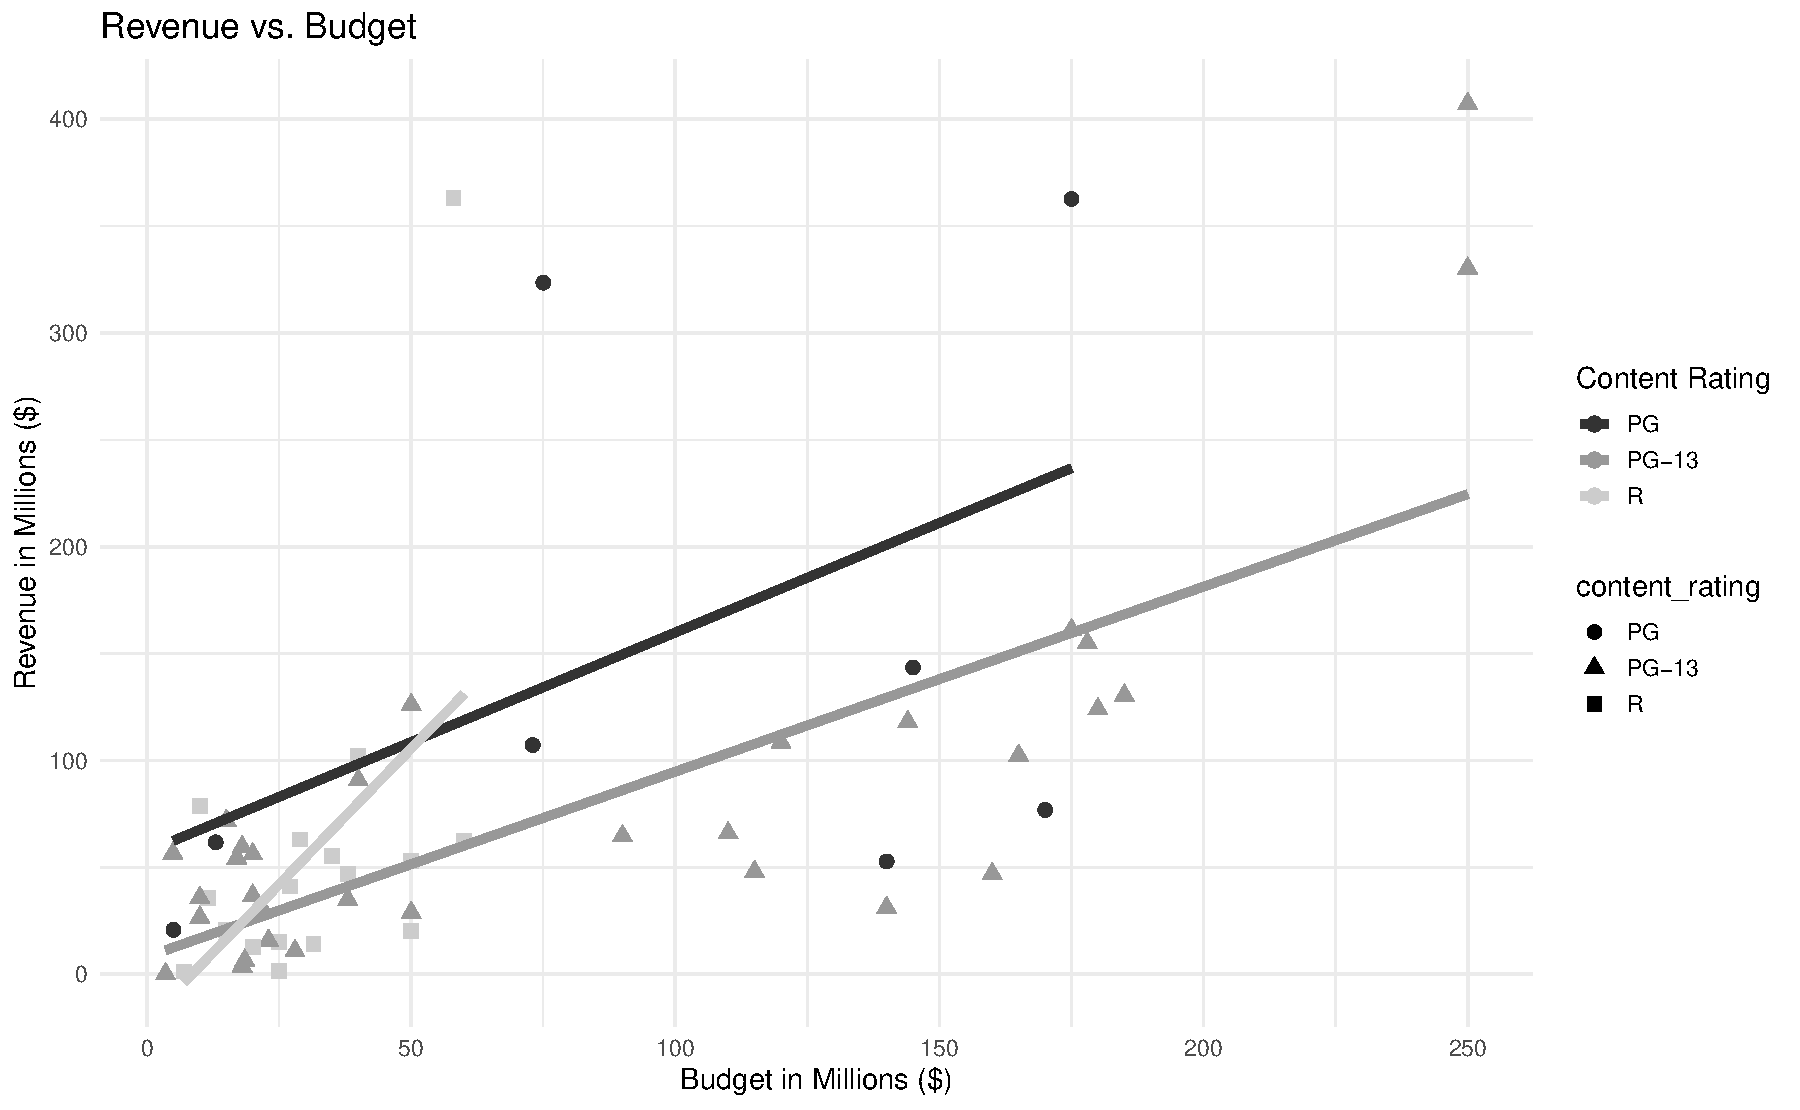
\includegraphics[width=0.7\linewidth]{05-EDA-multivariate_files/figure-latex/unnamed-chunk-5-1} \end{center}

\begin{enumerate}
\def\labelenumi{\arabic{enumi}.}
\setcounter{enumi}{3}
\tightlist
\item
  Identify the three variables plotted in this graph.
\end{enumerate}

\vspace{0.5in}

\begin{enumerate}
\def\labelenumi{\arabic{enumi}.}
\setcounter{enumi}{4}
\tightlist
\item
  Does the \emph{relationship} between movie budget and revenue differ among the different content ratings? Explain.
\end{enumerate}

\vspace{1in}

\hypertarget{take-home-messages}{%
\subsection{Take-home messages}\label{take-home-messages}}

\begin{enumerate}
\def\labelenumi{\arabic{enumi}.}
\item
  Two quantitative variables are graphically displayed in a scatterplot. The explanatory variable is on the \(x\)-axis and the response variable is on the \(y\)-axis. When describing the relationship between two quantitative variables we look at the form (linear or non-linear), direction (positive or negative), strength, and for the presence of outliers.
\item
  There are three summary statistics used to summarize the relationship between two quantitative variables: correlation (\(r\)), slope of the regression line (\(b_1\)), and the coefficient of determination (\(r^2\)).
\item
  The sign of correlation and the sign of the slope will always be the same. The closer the value of correlation is to \(-1\) or \(+1\), the stronger the relationship between the explanatory and the response variable.
\item
  The coefficient of determination multiplied by 100 (\(r^2 \times 100\)) measures the percent of variation in the response variable that is explained by the relationship with the explanatory variable. The closer the value of the coefficient of determination is to 100\%, the stronger the relationship.
\item
  We can use the line of regression to predict values of the response variable for values of the explanatory variable. Do not use values of the explanatory variable that are outside of the range of values in the data set to predict values of the response variable (why?). This is called \textbf{extrapolation}.
\end{enumerate}

\newpage

\hypertarget{additional-notes}{%
\subsection{Additional notes}\label{additional-notes}}

Use this space to summarize your thoughts and take additional notes on this week's activity and material covered.

\hypertarget{inference-for-a-single-categorical-variable-hypothesis-testing}{%
\chapter{Inference for a Single Categorical Variable: Hypothesis Testing}\label{inference-for-a-single-categorical-variable-hypothesis-testing}}

\hypertarget{reading-guide-categorical-inference}{%
\section{Reading Guide: Categorical Inference}\label{reading-guide-categorical-inference}}

\hypertarget{section-5.1-foundations-of-inference-hypothesis-tests}{%
\subsection*{Section 5.1 (Foundations of inference: Hypothesis tests)}\label{section-5.1-foundations-of-inference-hypothesis-tests}}
\addcontentsline{toc}{subsection}{Section 5.1 (Foundations of inference: Hypothesis tests)}

You may skip Section 5.1.4. This section will be covered next week.

\textbf{Videos}

\begin{itemize}
\tightlist
\item
  5.1
\end{itemize}

\setstretch{1.25}

\hypertarget{vocabulary}{%
\subsubsection*{Vocabulary}\label{vocabulary}}
\addcontentsline{toc}{subsubsection}{Vocabulary}

Statistical inference:
\rgs

Hypothesis test:

\rgi Also called a `significance test'.
\rgs

Simulation-based method:
\rgs

Theory-based method:
\rgs

Central Limit Theorem:
\rgs

Sampling distribution:
\rgs

Standard deviation of a statistic:
\rgs

Standard error of a statistic:
\rgs

Null hypothesis:
\rgs

Alternative hypothesis:
\rgs

P-value:
\rgs

Point estimate:
\rgs

Test statistic:
\rgs

Decision:
\rgs

Significance level (\(\alpha\)):
\rgs 

Statistically significant:
\rgs

\hypertarget{notes}{%
\subsubsection*{Notes}\label{notes}}
\addcontentsline{toc}{subsubsection}{Notes}

What `theory' is behind the theory-based methods of analysis?
\rgs

Consider the US judicial system:

\rgi What is the null hypothesis?
\rgs

\rgi What is the alternative hypothesis?
\rgs

\rgi The jury is presented with evidence.

~~~~~~~~~- If the evidence is strong (beyond a reasonable doubt), the jury will find the defendant:

\rgs

~~~~~~~~~- If the evidence is not strong (not beyond a reasonable doubt), the jury will find the defendant:

\rgs

To create a simulation, which hypothesis (null or alternative) do we assume is true?
\rgs

More on p-values:

\rgi Lower the p-value:
\rgs

\rgi Interpretations require:
\rgs

General steps of a hypothesis test:
\rgs

Conclusions should include:
\rgs

Decisions:

\rgi If p-value \(\leq \alpha\), the decision is to:

\rgi If p-value \(> \alpha\), the decision is to:

\newpage

True or False: If the p-value is above 0.10, that means the null hypothesis is true.

True or False: When conducting a simulation-based hypothesis test, the null hypothesis is assumed to be true to create the simulation.

\hypertarget{formulas}{%
\subsubsection*{Formulas}\label{formulas}}
\addcontentsline{toc}{subsubsection}{Formulas}

\(SD(\hat{p})\) =
\rgs

\hypertarget{example-martian-alphabet}{%
\subsubsection*{Example: Martian alphabet}\label{example-martian-alphabet}}
\addcontentsline{toc}{subsubsection}{Example: Martian alphabet}

\begin{enumerate}
\def\labelenumi{\arabic{enumi}.}
\item
  What is the sample statistic presented in this example? What notation would be used to represent this value?
  \rgs
\item
  What are the two possible explanations for how these data could have occurred?
  \rgs
\item
  Of the two explanations, which is the null and which is the alternative hypothesis?
  \rgs
\item
  How could coins be used to create a simulation of what should happen if everyone in the class was just guessing?
  \rgs
  \rgs
\item
  How can we use the simulation to determine which of the two possibilities is more believable?
  \rgs
  \rgs
\item
  What decision should be made at an \(\alpha = 0.05\) significance level? Justify your answer.
  \rgs
\item
  Are the results in this example statistically significant? Justify your answer.
  \rgs
\end{enumerate}

\hypertarget{section-5.2-the-normal-distribution}{%
\subsection*{Section 5.2 (The normal distribution)}\label{section-5.2-the-normal-distribution}}
\addcontentsline{toc}{subsection}{Section 5.2 (The normal distribution)}

\setstretch{1}

\textbf{Videos}

\begin{itemize}
\tightlist
\item
  5.2
\end{itemize}

\setstretch{1.25}

\hypertarget{vocabulary-1}{%
\subsubsection*{Vocabulary}\label{vocabulary-1}}
\addcontentsline{toc}{subsubsection}{Vocabulary}

Normal distribution:
\rgs

\rgi Notation:
\rgs

\rgi \rgi Also known as: normal curve, normal model, Gaussian distribution

\newpage

Standard normal distribution:
\rgs

\rgi Notation:
\rgs

Z-score:
\rgs

\(X\)th percentile:
\rgs

68-95-99.7 rule:
\rgs

\hypertarget{notes-1}{%
\subsubsection*{Notes}\label{notes-1}}
\addcontentsline{toc}{subsubsection}{Notes}

Interpretation of a Z-score:
\rgs

True or False: The more unusual observation will be the observation with the largest Z-score.

Approximately what percent of a normal distribution is in the interval

\rgi (mean -- standard deviation, mean + standard deviation):
\rgs

\rgi (mean -- 2\(\times\)(standard deviation), mean + 2\(\times\)(standard deviation)):
\rgs

\rgi (mean -- 3\(\times\)(standard deviation), mean + 3\(\times\)(standard deviation)):
\rgs

\hypertarget{formulas-1}{%
\subsubsection*{Formulas}\label{formulas-1}}
\addcontentsline{toc}{subsubsection}{Formulas}

Z =
\rgs

\hypertarget{r-coding}{%
\subsection*{\texorpdfstring{\texttt{R} coding}{R coding}}\label{r-coding}}
\addcontentsline{toc}{subsection}{\texttt{R} coding}

\hypertarget{calculating-normal-probabilities}{%
\paragraph{Calculating normal probabilities}\label{calculating-normal-probabilities}}
\addcontentsline{toc}{paragraph}{Calculating normal probabilities}

When using the \texttt{pnorm} \texttt{R} function, you will need to enter values for the arguments \texttt{mean}, \texttt{sd}, and \texttt{q} to match the question.

\begin{Shaded}
\begin{Highlighting}[]
\KeywordTok{pnorm}\NormalTok{(}\DataTypeTok{mean =}\NormalTok{ mu, }\DataTypeTok{sd =}\NormalTok{ sigma, }\DataTypeTok{q =}\NormalTok{ x, }\DataTypeTok{lower.tail =} \OtherTok{TRUE}\NormalTok{)}
\end{Highlighting}
\end{Shaded}

This function will return the proportion of the N(\texttt{mu},\texttt{sigma}) distribution which is \emph{below} the value \texttt{x}.

Example: \texttt{pnorm(mean\ =\ 5,\ sd\ =\ 2,\ q\ =\ 3,\ lower.tail\ =\ TRUE)} will give us the proportion of a N(5,2) distribution which is below 3, which equals 0.159:

\begin{Shaded}
\begin{Highlighting}[]
\KeywordTok{pnorm}\NormalTok{(}\DataTypeTok{mean =} \DecValTok{5}\NormalTok{, }\DataTypeTok{sd =} \DecValTok{2}\NormalTok{, }\DataTypeTok{q =} \DecValTok{3}\NormalTok{, }\DataTypeTok{lower.tail =} \OtherTok{TRUE}\NormalTok{)}
\CommentTok{#> [1] 0.1586553}
\end{Highlighting}
\end{Shaded}

Changing to \texttt{lower.tail\ =\ FALSE} will give the proportion of the distribution which is \emph{above} the value \texttt{x}.

\begin{Shaded}
\begin{Highlighting}[]
\KeywordTok{pnorm}\NormalTok{(}\DataTypeTok{mean =} \DecValTok{5}\NormalTok{, }\DataTypeTok{sd =} \DecValTok{2}\NormalTok{, }\DataTypeTok{q =} \DecValTok{3}\NormalTok{, }\DataTypeTok{lower.tail =} \OtherTok{FALSE}\NormalTok{)}
\CommentTok{#> [1] 0.8413447}
\end{Highlighting}
\end{Shaded}

\hypertarget{displaying-normal-probabilities}{%
\paragraph{Displaying normal probabilities}\label{displaying-normal-probabilities}}
\addcontentsline{toc}{paragraph}{Displaying normal probabilities}

When using the \texttt{normTail} \texttt{R} function, you will need to enter values for the arguments \texttt{m}, \texttt{s}, and \texttt{L} (or \texttt{U}) to match the question.

\begin{Shaded}
\begin{Highlighting}[]
\KeywordTok{normTail}\NormalTok{(}\DataTypeTok{m =}\NormalTok{ mu, }\DataTypeTok{s =}\NormalTok{ sigma, }\DataTypeTok{L =}\NormalTok{ x)}
\end{Highlighting}
\end{Shaded}

This function (in the \texttt{openintro} package) will plot a N(\texttt{mu}, \texttt{sigma}) distribution and shade the area that is below the value \texttt{x}.

Example: \texttt{normTail(m\ =\ 5,\ s\ =\ 2,\ L\ =\ 3)} creates the plot pictured below.

\begin{figure}

{\centering 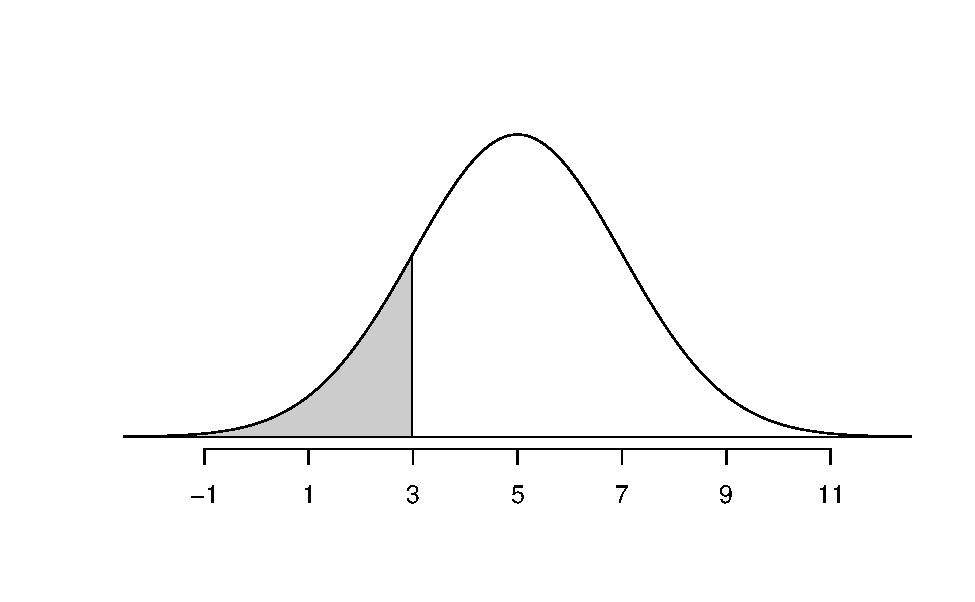
\includegraphics[width=0.6\linewidth]{06-inference-1cat_test_files/figure-latex/normgt3-1} 

}

\end{figure}

Changing \texttt{L} to \texttt{U} will shade the area \emph{above} \texttt{x}.

Example: \texttt{normTail(m\ =\ 5,\ s\ =\ 2,\ U\ =\ 3)} plots a N(5,2) distribution with the area above 3 shaded.

\hypertarget{calculating-normal-percentiles}{%
\paragraph{Calculating normal percentiles}\label{calculating-normal-percentiles}}
\addcontentsline{toc}{paragraph}{Calculating normal percentiles}

When using the \texttt{qnorm} \texttt{R} function, you will need to enter values for the arguments \texttt{mean}, \texttt{sd}, and \texttt{p} to match the question.

\begin{Shaded}
\begin{Highlighting}[]
\KeywordTok{qnorm}\NormalTok{(}\DataTypeTok{mean =}\NormalTok{ mu, }\DataTypeTok{sd =}\NormalTok{ sigma, }\DataTypeTok{p =}\NormalTok{ x, }\DataTypeTok{lower.tail =} \OtherTok{TRUE}\NormalTok{)}
\end{Highlighting}
\end{Shaded}

This function will return the value on the N(\texttt{mu}, \texttt{sigma}) distribution which has \texttt{x} area of the distribution \emph{below} it.

Example: \texttt{qnorm(mean\ =\ 5,\ sd\ =\ 2,\ p\ =\ 0.159,\ lower.tail\ =\ TRUE)} will give us the value on a N(5,2) distribution which has 0.159 (15.9\%) of the distribution below it, which equals 3 (from the \texttt{R} output above).

Changing to \texttt{lower.tail\ =\ FALSE} will give the value which has \texttt{x} area of the distribution \emph{above} it.

We would recommend you work through each of the examples in Section 5.2.4 using \texttt{R}.

\hypertarget{section-5.3-inference-for-one-proportion}{%
\subsection*{Section 5.3 (Inference for one proportion)}\label{section-5.3-inference-for-one-proportion}}
\addcontentsline{toc}{subsection}{Section 5.3 (Inference for one proportion)}

\setstretch{1}

You may skip Section 5.3.2 and stop before the ``Confidence interval for \(\pi\)'' sub-section in Section 5.3.3. These sections will be covered next week.

\textbf{Videos}

\begin{itemize}
\tightlist
\item
  5.3
\item
  OnePropTheory
\end{itemize}

\setstretch{1.25}

\hypertarget{reminders-from-previous-sections}{%
\subsubsection*{Reminders from previous sections}\label{reminders-from-previous-sections}}
\addcontentsline{toc}{subsubsection}{Reminders from previous sections}

\(n\) = sample size

\(\hat{p}\) = sample proportion

\(\pi\) = population proportion

General steps of a hypothesis test:

\begin{enumerate}
\def\labelenumi{\arabic{enumi}.}
\item
  Frame the research question in terms of hypotheses.
\item
  Collect and summarize data using a test statistic.
\item
  Assume the null hypothesis is true, and simulate or mathematically model a null distribution for the test statistic.
\item
  Compare the observed test statistic to the null distribution to calculate a p-value.
\item
  Make a conclusion based on the p-value and write the conclusion in context.
\end{enumerate}

Parameter: a value summarizing a variable(s) for a population.

Statistic: a value summarizing a variable(s) for a sample.

Sampling distribution: plot of statistics from 1000s of samples of the same size taken from the same population.

Standard deviation of a statistic: the variability of statistics from 1000s of samples. How far, on average, each statistic is from the true value of the parameter.

Standard error of a statistic: estimated standard deviation of a statistic.

Hypothesis test: a process to determine how strong the evidence of an effect is.

\rgi Also called a `significance test'.

Simulation-based method: Simulate lots of samples of size \(n\) under assumption of the null hypothesis, then find the proportion of the simulations that are at least as extreme as the observed sample statistic.

Theory-based method: Develop a mathematical model for the statistic under the null hypothesis and use the model to calculate the probability of the observed sample statistic (or one more extreme) occurring.

Null hypothesis: \(H_0\) the skeptical perspective; no difference; no change; no effect; random chance; what the researcher hopes to prove is \textbf{wrong}.

Alternative hypothesis: \(H_A\) the new perspective; a difference/increase/decrease; an effect; not random chance; what the researcher hopes to prove is \textbf{correct}.

P-value: probability of seeing the observed sample data, or something more extreme, assuming the null hypothesis is true.

\(\implies\) Lower the p-value the stronger the evidence AGAINST the null hypothesis and FOR the alternative hypothesis.

Decision: a determination of whether to `reject' or `fail to reject' a null hypothesis based on a p-value and a pre-set level of significance.

Significance level (\(\alpha\)): a threshold used to determine if a p-value provides enough evidence to reject the null hypothesis or not.

\rgi Common levels of \(\alpha\) include 0.01, 0.05, and 0.10.

Statistically significant: results are considered statistically significant if the p-value is below the significance level.

Central Limit Theorem: For large sample sizes, the sampling distribution of a sample proportion (or mean) will be approximately normal (bell-shaped and symmetric).

\hypertarget{vocabulary-2}{%
\subsubsection*{Vocabulary}\label{vocabulary-2}}
\addcontentsline{toc}{subsubsection}{Vocabulary}

Point estimate:
\rgs

Test statistic:
\rgs

Null value:
\rgs

Null distribution:
\rgs

Standardized statistic:
\rgs

\hypertarget{notes-2}{%
\subsubsection*{Notes}\label{notes-2}}
\addcontentsline{toc}{subsubsection}{Notes}

Conditions for the Central Limit Theorem to apply (for the sampling distribution of \(\hat{p}\) to be approximately normal)

\rgi Independence:
\rgs

\rgi \rgi Checked by:
\rgs

\rgi Success-failure condition:
\rgs

\rgi \rgi Checked by:
\rgs

\hypertarget{formulas-2}{%
\subsubsection*{Formulas}\label{formulas-2}}
\addcontentsline{toc}{subsubsection}{Formulas}

\(SD(\hat{p})\) =
\rgs

Null standard error of the sample proportion:

\(SE_0(\hat{p})\) =
\rgs

Standardized statistic/standardized sample proportion:

\(Z\) =
\rgs

\hypertarget{example-organ-donations}{%
\subsubsection*{Example: Organ donations}\label{example-organ-donations}}
\addcontentsline{toc}{subsubsection}{Example: Organ donations}

\begin{enumerate}
\def\labelenumi{\arabic{enumi}.}
\item
  What is the sample statistic presented in this example? What notation would be used to represent this value?
  \rgs
\item
  What is the parameter representing in the context of this problem? What notation would be used to represent this parameter?
  \rgs
\item
  Write the null and alternative hypotheses in words.
  \rgs
\item
  Write the null and alternative hypotheses in notation.
  \rgs
\item
  To simulate the null distribution, we would not be able to use coins. Why or why not?
  \rgs
\item
  How could we use cards to simulate 1 sample which assumes the null hypothesis is true? How many blue cards --- to represent what? How many red cards --- to represent what? How many times would we draw a card and replace it back in the deck? What would you record once you completed the draw-with-replacement process?
  \rgs
\item
  How can we calculate a p-value from the simulated null distribution for this example?
  \rgs
\item
  What was the p-value of the test?
  \rgs
\item
  At the 5\% significance level, what decision would you make?
  \rgs
\item
  What conclusion should the researcher make?
  \rgs
\item
  Are the results in this example statistically significant? Justify your answer.
  \rgs
\item
  Are the conditions met to use theoretical methods to analyze these data?
  \rgs
\end{enumerate}

\hypertarget{example-payday-loans}{%
\subsubsection*{Example: Payday loans}\label{example-payday-loans}}
\addcontentsline{toc}{subsubsection}{Example: Payday loans}

\begin{enumerate}
\def\labelenumi{\arabic{enumi}.}
\item
  What is the parameter representing in the context of this problem? What notation would be used to represent this parameter?
  \rgs
\item
  Write the null and alternative hypotheses in words.
  \rgs
\item
  Write the null and alternative hypotheses in notation.
  \rgs
\item
  Are the conditions met to use theoretical methods to analyze these data?
  \rgs
\item
  Calculate the null standard error of the sample proportion.
  \rgs
\item
  What is the sample statistic presented in this example? What notation would be used to represent this value?
  \rgs
\item
  Calculate the standardized sample proportion.
  \rgs
\item
  How can we calculate a p-value from the normal distribution for this example?
  \rgs
\item
  What was the p-value of the test?
  \rgs
\item
  At the 5\% significance level, what decision would you make?
  \rgs
\item
  What conclusion should the researcher make?
  \rgs
\item
  Are the results in this example statistically significant? Justify your answer.
  \rgs
\end{enumerate}

\newpage

\hypertarget{activity-handedness-of-male-boxers-testing}{%
\section{Activity: Handedness of Male Boxers --- Testing}\label{activity-handedness-of-male-boxers-testing}}

\setstretch{1}

\hypertarget{learning-objectives}{%
\subsection{Learning objectives}\label{learning-objectives}}

\begin{itemize}
\item
  Identify the two possible explanations (one assuming the null hypothesis, and one assuming the alternative hypothesis) for a relationship seen in sample data.
\item
  Given a research question involving a single categorical variable, construct the null and alternative hypotheses
  in words and using appropriate statistical symbols.
\item
  Describe and perform a simulation-based hypothesis test for a single proportion.
\item
  Interpret and evaluate a p-value for a simulation-based hypothesis test for a single proportion.
\end{itemize}

\hypertarget{terminology-review}{%
\subsection{Terminology review}\label{terminology-review}}

In this week's in-class activity, we will introduce simulation-based hypothesis testing for a single categorical variable. Some terms covered in this activity are:

\begin{itemize}
\item
  Parameter of interest
\item
  Null hypothesis
\item
  Alternative hypothesis
\item
  Simulation
\item
  Null distribution
\item
  p-value
\end{itemize}

To review these concepts, see Chapter 5 in your textbook, focusing on Sections 5.1 through 5.3.

\hypertarget{steps-of-the-statistical-investigation-process}{%
\subsection{Steps of the statistical investigation process}\label{steps-of-the-statistical-investigation-process}}

We will work through a six-step process to complete a hypothesis test for a single proportion, first introduced in the Martian Alphabet Activity in week 1.

\begin{itemize}
\item
  \textbf{Ask a research question} that can be addressed by collecting data. What are the researchers trying to show?
\item
  \textbf{Design a study and collect data}. This step involves selecting the people or objects to be studied and how to gather relevant data on them.
\item
  \textbf{Summarize and visualize the data}. Calculate summary statistics and create graphical plots that best represent the research question.
\item
  \textbf{Use statistical analysis methods to draw inferences from the data}. Choose an statistical inference method appropriate for the data and identify the p-value and/or confidence interval after checking assumptions. In this study, we will focus on using randomization to generate a simulated p-value.
\item
  \textbf{Communicate the results and answer the research question}. Using the p-value and confidence interval from the analysis, determine whether the data provide statistical evidence against the null hypothesis. Write a conclusion that addresses the research question.
\item
  \textbf{Revisit and look forward} to point out limitations of the study and suggest new studies that could be performed to build on the findings of the study.
\end{itemize}

\newpage

\hypertarget{handedness-of-male-boxers}{%
\subsection{Handedness of male boxers}\label{handedness-of-male-boxers}}

Left-handedness is a trait that is found in about 10\% of the population. Past studies have shown that left-handed men are over-represented among professional boxers. The fighting claim states that left-handed men have an advantage in competition. In this random sample of 500 male professional boxers, we want to see if there is an over-prevalence of left-handed fighters.

\hypertarget{summary-statistics-review.-complete-q1q4-before-class.}{%
\subsubsection*{Summary statistics review. Complete Q1--Q4 before class.}\label{summary-statistics-review.-complete-q1q4-before-class.}}
\addcontentsline{toc}{subsubsection}{Summary statistics review. Complete Q1--Q4 before class.}

\begin{enumerate}
\def\labelenumi{\arabic{enumi}.}
\tightlist
\item
  What are the observational units?
\end{enumerate}

\vspace{0.5in}

\begin{enumerate}
\def\labelenumi{\arabic{enumi}.}
\setcounter{enumi}{1}
\tightlist
\item
  What variable are we measuring on each observational unit? Is it categorical or quantitative?
\end{enumerate}

\vspace{0.5in}

\begin{enumerate}
\def\labelenumi{\arabic{enumi}.}
\setcounter{enumi}{2}
\tightlist
\item
  What type of plot would be appropriate to visually display these data?
\end{enumerate}

\vspace{0.5in}

\begin{enumerate}
\def\labelenumi{\arabic{enumi}.}
\setcounter{enumi}{3}
\tightlist
\item
  Write out in context the statistic we will calculate to summarize the data.
\end{enumerate}

\vspace{0.5in}

\hypertarget{ask-a-research-question}{%
\subsubsection*{Ask a research question}\label{ask-a-research-question}}
\addcontentsline{toc}{subsubsection}{Ask a research question}

\begin{enumerate}
\def\labelenumi{\arabic{enumi}.}
\setcounter{enumi}{4}
\tightlist
\item
  Identify the research question for this study.
\end{enumerate}

\vspace{1in}

\hypertarget{design-a-study-and-collect-data}{%
\subsubsection*{Design a study and collect data}\label{design-a-study-and-collect-data}}
\addcontentsline{toc}{subsubsection}{Design a study and collect data}

Before using statistical inference methods, we must check that the cases are independent. The sample observations are independent if the outcome of one observation does not influence the outcome of another. One way this condition is met is if data come from a simple random sample of the target population.

\begin{enumerate}
\def\labelenumi{\arabic{enumi}.}
\setcounter{enumi}{5}
\tightlist
\item
  Are the cases independent? Justify your answer.
\end{enumerate}

\vspace{1in}

\newpage

\hypertarget{summarize-and-visualize-the-data}{%
\subsubsection*{Summarize and visualize the data}\label{summarize-and-visualize-the-data}}
\addcontentsline{toc}{subsubsection}{Summarize and visualize the data}

\begin{Shaded}
\begin{Highlighting}[]
\NormalTok{handedness <-}\StringTok{ }\KeywordTok{read.csv}\NormalTok{(}\StringTok{"data/Male_boxers_sample.csv"}\NormalTok{) }\CommentTok{# Read in data set}
\NormalTok{handedness }\OperatorTok\StringTok{ }\KeywordTok{count}\NormalTok{(Stance)  }\CommentTok{# Count number in each Stance category}
\end{Highlighting}
\end{Shaded}

\begin{verbatim}
#>         Stance   n
#> 1  left-handed  81
#> 2 right-handed 419
\end{verbatim}

\begin{enumerate}
\def\labelenumi{\arabic{enumi}.}
\setcounter{enumi}{6}
\tightlist
\item
  Using the output above, calculate the appropriate summary statistic to represent the research question. Use appropriate notation.
\end{enumerate}

\vspace{0.5in}

\begin{enumerate}
\def\labelenumi{\arabic{enumi}.}
\setcounter{enumi}{7}
\tightlist
\item
  What type of plot should be used to represent these data? Sketch this plot.
\end{enumerate}

\vspace{1.5in}

\hypertarget{use-statistical-analysis-methods-to-draw-inferences-from-the-data}{%
\subsubsection*{Use statistical analysis methods to draw inferences from the data}\label{use-statistical-analysis-methods-to-draw-inferences-from-the-data}}
\addcontentsline{toc}{subsubsection}{Use statistical analysis methods to draw inferences from the data}

When performing a hypothesis test, we must first identify the null hypothesis. The null hypothesis is written about the parameter of interest, or the value that summarizes the variable in the population. \emph{For example, in the Martian Alphabet Activity, the parameter of interest is the true proportion of statistic students who would correctly identify Bumba.}

\begin{enumerate}
\def\labelenumi{\arabic{enumi}.}
\setcounter{enumi}{8}
\tightlist
\item
  Write out the parameter of interest for this study.
\end{enumerate}

\vspace{0.8in}

\begin{enumerate}
\def\labelenumi{\arabic{enumi}.}
\setcounter{enumi}{9}
\tightlist
\item
  Using the parameter of interest in question 9, write out the null hypothesis in words. That is, what do we assume to be true about the parameter of interest when we perform our simulation?
\end{enumerate}

\vspace{0.8in}

The notation used for a population proportion (or probability, or true proportion) is \(\pi\). Since this summarizes a population, it is a parameter. When writing the \textbf{null hypothesis} in notation, we set the parameter equal to the null value, \(H_0: \pi = \pi_0\).

\begin{enumerate}
\def\labelenumi{\arabic{enumi}.}
\setcounter{enumi}{10}
\tightlist
\item
  Write the null hypothesis in notation using the null value of 0.1 in place of \(\pi_0\) in the equation given above.
\end{enumerate}

\vspace{0.5in}

\newpage

The \textbf{alternative hypothesis} is the claim to be tested and the direction of the claim (less than, greater than, or not equal to) is based on the research question.

\begin{enumerate}
\def\labelenumi{\arabic{enumi}.}
\setcounter{enumi}{11}
\tightlist
\item
  Based on the research question from question 5, are we testing that the parameter is greater than 0.1, less than 0.1 or different than 0.1?
\end{enumerate}

\vspace{0.4in}

\begin{enumerate}
\def\labelenumi{\arabic{enumi}.}
\setcounter{enumi}{12}
\tightlist
\item
  Write out the alternative hypothesis in words.
\end{enumerate}

\vspace{1in}

\begin{enumerate}
\def\labelenumi{\arabic{enumi}.}
\setcounter{enumi}{13}
\tightlist
\item
  Write out the alternative hypothesis in notation.
\end{enumerate}

\vspace{0.5in}

Remember that when utilizing a hypothesis test, we are evaluating two competing possibilities. For this study the \textbf{two possibilities} are either\ldots{}

\begin{itemize}
\item
  The true proportion of male boxers who are left-handed is 0.1 and our results just occurred by random chance; or,
\item
  The true proportion of male boxers who are left-handed is greater than 0.1 and our results reflect this.
\end{itemize}

Notice that these two competing possibilities represent the null and alternative hypotheses.

We will now simulate a \textbf{null distribution} of sample proportions. The null distribution is created under the assumption the null hypothesis is true. In this case, we assume the true proportion of male boxers who are left-handed is 0.1, so we will create 1000 (or more) different simulations of 500 boxers under this assumption.

Let's think about how to use red and blue cards to create one simulation of 500 boxers under the assumption the null hypothesis is true. Suppose blue cards represents left-handed boxers and red cards represents right-handed boxers.

\begin{enumerate}
\def\labelenumi{\arabic{enumi}.}
\setcounter{enumi}{14}
\tightlist
\item
  How many cards total do we need? How many blue ones? How many red ones?
\end{enumerate}

\vspace{0.5in}

\begin{enumerate}
\def\labelenumi{\arabic{enumi}.}
\setcounter{enumi}{15}
\tightlist
\item
  Next, we would mix the cards together and draw 1 card, write down if it's red or blue, and replace the card. How many times would we need to repeat this process to simulate one sample?
\end{enumerate}

\vspace{0.5in}

\begin{enumerate}
\def\labelenumi{\arabic{enumi}.}
\setcounter{enumi}{16}
\tightlist
\item
  Once we have one simulated sample, what would we calculate and plot on the null distribution? \emph{Hint}: What statistic are we calculating from the data?
\end{enumerate}

\vspace{1in}

We will use the computer to simulate a null distribution of 1000 different samples of 500 male boxers, plotting the proportion who are left-handed in each sample, based on the assumption that the true proportion of male boxers who are left-handed is 0.1 (or that the null hypothesis is true).

To use the computer simulation, we will need to enter the

\begin{itemize}
\tightlist
\item
  assumed ``probability of success'' (\(\pi_0\)),
\item
  ``sample size'' (the number of observational units or cases in the sample),
\item
  ``number of repetitions'' (the number of samples to be generated),
\item
  ``as extreme as'' (the observed statistic), and
\item
  the ``direction'' (matches the direction of the alternative hypothesis).
\end{itemize}

\begin{enumerate}
\def\labelenumi{\arabic{enumi}.}
\setcounter{enumi}{17}
\tightlist
\item
  What values should be entered for each of the following into the one proportion test to create 1000 simulations?
\end{enumerate}

\vspace{1mm}

\begin{itemize}
\tightlist
\item
  Probability of success:
\end{itemize}

\vspace{.2in}

\begin{itemize}
\tightlist
\item
  Sample size:
\end{itemize}

\vspace{.2in}

\begin{itemize}
\tightlist
\item
  Number of repetitions:
\end{itemize}

\vspace{.2in}

\begin{itemize}
\tightlist
\item
  As extreme as:
\end{itemize}

\vspace{.2in}

\begin{itemize}
\tightlist
\item
  Direction (\texttt{"greater"}, \texttt{"less"}, or \texttt{"two-sided"}):
\end{itemize}

\vspace{.2in}

Using the provided \texttt{R} script file, fill in the values/words for each \texttt{xx} with your answers from question 18 in the one proportion test to create a null distribution with 1000 simulations. Then highlight and run lines 1--14.

\begin{Shaded}
\begin{Highlighting}[]
\KeywordTok{one_proportion_test}\NormalTok{(}\DataTypeTok{probability_success =}\NormalTok{ xx, }\CommentTok{# Null hypothesis value}
                    \DataTypeTok{sample_size =}\NormalTok{ xx, }\CommentTok{# Enter sample size}
                    \DataTypeTok{number_repetitions =} \DecValTok{1000}\NormalTok{, }\CommentTok{# Enter number of simulations}
                    \DataTypeTok{as_extreme_as =}\NormalTok{ xx, }\CommentTok{# Observed statistic}
                    \DataTypeTok{direction =} \StringTok{"xx"}\NormalTok{, }\CommentTok{# Specify direction of alternative hypothesis}
                    \DataTypeTok{report_value =} \StringTok{"proportion"}\NormalTok{) }\CommentTok{# Reporting proportion or number of successes?}
\end{Highlighting}
\end{Shaded}

\begin{enumerate}
\def\labelenumi{\arabic{enumi}.}
\setcounter{enumi}{18}
\tightlist
\item
  Sketch the null distribution created from the \texttt{R} code here.
\end{enumerate}

\vspace{1.8in}

\begin{enumerate}
\def\labelenumi{\arabic{enumi}.}
\setcounter{enumi}{19}
\tightlist
\item
  Around what value is the null distribution centered? Why does that make sense?
\end{enumerate}

\vspace{1in}

\begin{enumerate}
\def\labelenumi{\arabic{enumi}.}
\setcounter{enumi}{20}
\tightlist
\item
  Circle the observed statistic (value from question 7) on the distribution you drew in question 19. Where does this statistic fall in the null distribution: Is it near the center of the distribution (near 0.1) or in one of the tails of the distribution?
\end{enumerate}

\vspace{1in}

\begin{enumerate}
\def\labelenumi{\arabic{enumi}.}
\setcounter{enumi}{21}
\tightlist
\item
  Is the observed statistic likely to happen or unlikely to happen if the true proportion of male boxers who are left-handed is 0.1? Explain your answer using the plot.
\end{enumerate}

\vspace{1in}

\begin{enumerate}
\def\labelenumi{\arabic{enumi}.}
\setcounter{enumi}{22}
\tightlist
\item
  Using the simulation, what is the proportion of simulated samples that generated a sample proportion at the observed statistic or greater, if the true proportion of male boxers who are left-handed is 0.1? \emph{Hint}: Look under the simulation.
\end{enumerate}

\vspace{1in}

The value in question 23 is the \textbf{p-value}. The smaller the p-value, the more evidence we have against the null hypothesis. (Why?)

\begin{enumerate}
\def\labelenumi{\arabic{enumi}.}
\setcounter{enumi}{23}
\tightlist
\item
  Using the following guidelines for the strength of evidence, how much evidence do the data provide against the null hypothesis? (Circle one of the five descriptions.)
\end{enumerate}

\begin{center}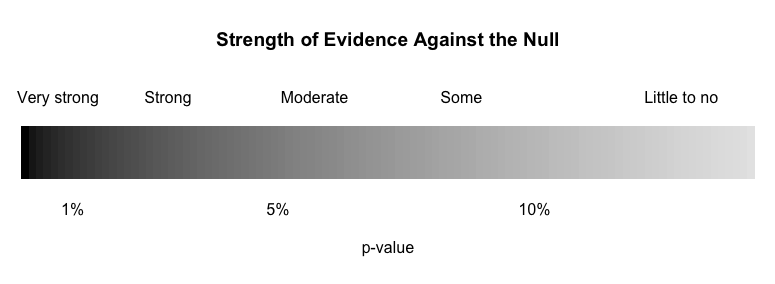
\includegraphics[width=0.9\linewidth]{images/soe_gradient_grayscale} \end{center}

\begin{enumerate}
\def\labelenumi{\arabic{enumi}.}
\setcounter{enumi}{24}
\tightlist
\item
  What does the p-value measure?: Interpret the p-value in context of the problem.
\end{enumerate}

\vspace{1in}

\hypertarget{communicate-the-results-and-answer-the-research-question}{%
\subsubsection*{Communicate the results and answer the research question}\label{communicate-the-results-and-answer-the-research-question}}
\addcontentsline{toc}{subsubsection}{Communicate the results and answer the research question}

When we write a conclusion we answer the research question by stating how much evidence there is for the alternative hypothesis.

\begin{enumerate}
\def\labelenumi{\arabic{enumi}.}
\setcounter{enumi}{25}
\tightlist
\item
  Write a conclusion in context of the study.
\end{enumerate}

\vspace{1in}

\begin{enumerate}
\def\labelenumi{\arabic{enumi}.}
\setcounter{enumi}{26}
\tightlist
\item
  Write a paragraph summarizing the results as if you were writing a press release. Be sure to describe:
\end{enumerate}

\begin{itemize}
\item
  Summary statistic
\item
  P-value and interpretation
\item
  Conclusion (written to answer the research question)
\item
  Generalization --- to what group do the results apply?
\end{itemize}

\vspace{4in}

\hypertarget{revisit-and-look-forward}{%
\subsubsection*{Revisit and look forward}\label{revisit-and-look-forward}}
\addcontentsline{toc}{subsubsection}{Revisit and look forward}

\begin{enumerate}
\def\labelenumi{\arabic{enumi}.}
\setcounter{enumi}{27}
\tightlist
\item
  Suggest a new research question that you might investigate, building on what you learned in this study.
\end{enumerate}

\vspace{.6in}

\newpage

\hypertarget{out-of-class-activity}{%
\subsection{Out-of-class activity}\label{out-of-class-activity}}

The in-class activity covered simulation-based methods for hypothesis tests involving a single categorical variable. The remaining questions cover theory-based methods for testing a single categorical variable. Use Section 5.3.3 in the textbook and the OnePropTheory video to complete the following questions.

The sampling distribution of a single proportion --- how that proportion varies from sample to sample --- can be mathematically modeled using the normal distribution if certain conditions are met.

Conditions for the sampling distribution of \(\hat{p}\) to follow an approximate normal distribution:

\begin{itemize}
\item
  \textbf{Independence}: The sample's observations are independent, e.g., are from a simple random sample.
\item
  \textbf{Success-failure condition}: We \emph{expect} to see at least 10 successes and 10 failures in the sample, \(n\pi≥10\) and \(n(1-\pi)≥10\).
\end{itemize}

\begin{enumerate}
\def\labelenumi{\arabic{enumi}.}
\tightlist
\item
  We already verified that the independence condition is satisfied in question 6, since the independence condition is required for both simulation-based and theory-based methods. Is the success-failure condition met to model the data with the normal distribution? Show your work to support your answer. Hint: We don't know the true value of the parameter, \(\pi\), so we use the null value, \(\pi_0\), to check the success-failure condition.
\end{enumerate}

\vspace{1in}

To calculate the standardized statistic we use the general formula

\[
Z = \frac{\text{point estimate} - \text{null value}}{SE_0(\text{point estimate})}.
\]
For a single categorical variable the standardized sample proportion is calculated using

\[
Z = \frac{\hat{p} - \pi_0}{SE_0(\hat{p})},
\]
where the standard error is calculated using the null value:

\[SE_0(\hat{p})=\sqrt{\frac{\pi_0(1-\pi_0)}{n}}\].
\vspace{0.5mm}

\begin{enumerate}
\def\labelenumi{\arabic{enumi}.}
\setcounter{enumi}{1}
\tightlist
\item
  Calculate the null standard error of the sample proportion.
\end{enumerate}

\vspace{1in}

\begin{enumerate}
\def\labelenumi{\arabic{enumi}.}
\setcounter{enumi}{2}
\tightlist
\item
  Calculate the standardized sample proportion.
\end{enumerate}

\vspace{1in}

\newpage

The standardized statistic is used as a ruler to measure how far the sample statistic is from the null value. Essentially, we are converting the sample proportion into a measure of standard errors to compare to the standard normal distribution.

\begin{figure}

{\centering 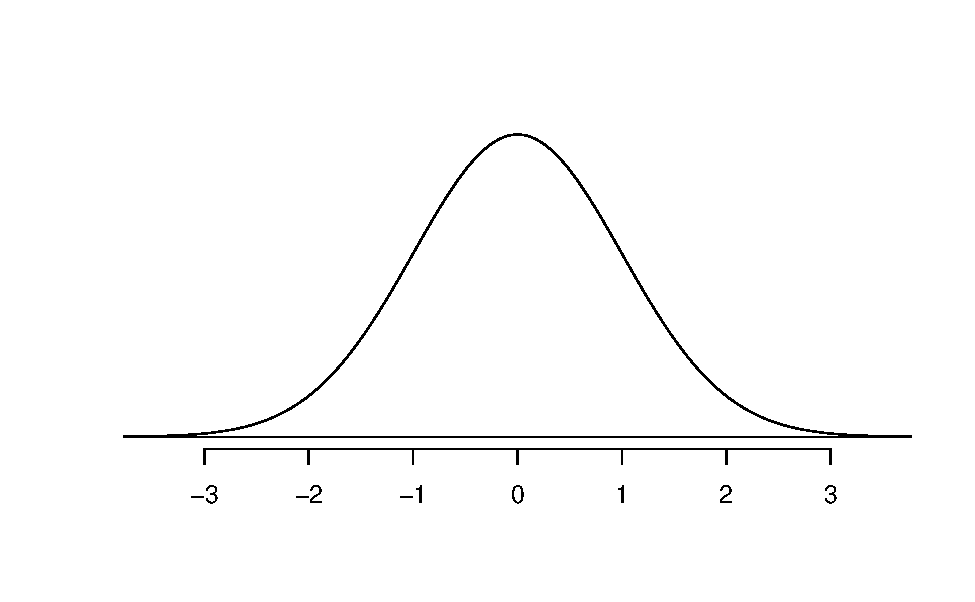
\includegraphics[width=0.7\linewidth]{06-inference-1cat_test_files/figure-latex/simpleNormal-1} 

}

\caption{A standard normal curve.}\label{fig:simpleNormal}
\end{figure}

\begin{enumerate}
\def\labelenumi{\arabic{enumi}.}
\setcounter{enumi}{3}
\tightlist
\item
  Using the 68-95-99.7 rule in Section 5.2.5 to guide you, fill in values on the \(x\)-axis of the standard normal distribution displayed in Figure \ref{fig:simpleNormal}, and mark on the value of the standardized statistic calculated in question 3.
\end{enumerate}

\vspace{0.2in}

The standardized statistic measures the \emph{number of standard errors the sample statistic is from the null value}.

\begin{enumerate}
\def\labelenumi{\arabic{enumi}.}
\setcounter{enumi}{4}
\tightlist
\item
  Interpret the standardized sample proportion from question 3 in context of the problem.
\end{enumerate}

\vspace{1in}

We will use the \texttt{pnorm} function in \texttt{R} to find the p-value. Use the provided \texttt{R} script file and enter the value of the standardized statistic calculated in question 3 at xx in line 18; highlight and run lines 18--20. Notice that in line 20 it says \texttt{lower.tail\ =\ FALSE}. \texttt{R} will calculate the p-value \emph{greater} than the value of the standardized statistic.

Notes:

\begin{itemize}
\tightlist
\item
  Use \texttt{lower.tail\ =\ TRUE} when doing a left-sided test.
\item
  Use \texttt{lower.tail\ =\ FALSE} when doing a right-sided test.
\item
  To find a two-sided p-value, use a left-sided test for negative Z or a right-sided test for positive Z, then multiply the value found by 2 to get the p-value.
\end{itemize}

\begin{Shaded}
\begin{Highlighting}[]
\KeywordTok{pnorm}\NormalTok{(xx, }\CommentTok{# Enter value of standardized statistic}
      \DataTypeTok{m=}\DecValTok{0}\NormalTok{, }\DataTypeTok{s=}\DecValTok{1} \CommentTok{# Using the standard normal mean = 0, sd = 1}
      \DataTypeTok{lower.tail=}\OtherTok{FALSE}\NormalTok{) }\CommentTok{# Gives a p-value greater than the standardized statistic}
\end{Highlighting}
\end{Shaded}

\begin{enumerate}
\def\labelenumi{\arabic{enumi}.}
\setcounter{enumi}{5}
\item
  Report the p-value obtained from the \texttt{R} output.
  \vspace{0.2in}
\item
  Is the p-value found in question 6 similar to the p-value found using the simulation test? Explain why you would expect this to be true.
\end{enumerate}

\vspace{0.5in}

\newpage

\hypertarget{take-home-messages}{%
\subsection{Take-home messages}\label{take-home-messages}}

\begin{enumerate}
\def\labelenumi{\arabic{enumi}.}
\item
  In a hypothesis test we have two competing hypotheses, the null hypothesis and the alternative hypothesis. The null hypothesis represents either a skeptical perspective or a perspective of no difference or no effect. The alternative hypothesis represents a new perspective such as the possibility that there has been a change or that there is a treatment effect in an experiment.
\item
  In a simulation-based test, we create a distribution of possible simulated statistics for our sample if the null hypothesis is true. Then we see if the calculated observed statistic from the data is likely or unlikely to occur when compared to the null distribution.
\item
  The p-value is the probability of the observed statistic occurring or more extreme if the null hypothesis is true. The farther in the tail of the distribution the observed statistic is, the smaller the probability is (smaller the p-value!). The \textbf{smaller} the p-value, the \textbf{more} evidence the statistic provides \textbf{against} the null hypothesis. (Think carefully about why this makes sense!)
\item
  A `decision' is a statement about strength of evidence against the null hypothesis: reject the null if the p-value is below a pre-set significance level, and fail to reject the null if the p-value is above a pre-set significance level. When writing a `conclusion' to a hypothesis test, on the other hand, we are answering the research question. Thus, a conclusion is a statement about strength of evidence \emph{for the alternative hypothesis}. Use the guidelines for the strength of evidence throughout this course to assess the evidence against the null hypothesis.
\end{enumerate}

\hypertarget{additional-notes}{%
\subsection{Additional notes}\label{additional-notes}}

Use this space to summarize your thoughts and take additional notes on this week's activity and material covered.

\hypertarget{inference-for-a-single-categorical-variable-confidence-intervals}{%
\chapter{Inference for a Single Categorical Variable: Confidence Intervals}\label{inference-for-a-single-categorical-variable-confidence-intervals}}

\hypertarget{reading-guide-categorical-inference}{%
\section{Reading Guide: Categorical Inference}\label{reading-guide-categorical-inference}}

\hypertarget{section-5.1.4-foundations-of-inference-confidence-intervals}{%
\subsection*{Section 5.1.4 (Foundations of inference: Confidence intervals)}\label{section-5.1.4-foundations-of-inference-confidence-intervals}}
\addcontentsline{toc}{subsection}{Section 5.1.4 (Foundations of inference: Confidence intervals)}

\textbf{Videos}

\begin{itemize}
\tightlist
\item
  5.1
\end{itemize}

\setstretch{1.25}

\hypertarget{vocabulary}{%
\subsubsection*{Vocabulary}\label{vocabulary}}
\addcontentsline{toc}{subsubsection}{Vocabulary}

Confidence interval:
\rgs

Margin of error:
\rgs

\hypertarget{formulas}{%
\subsubsection*{Formulas}\label{formulas}}
\addcontentsline{toc}{subsubsection}{Formulas}

General form of a theory-based confidence interval:
\rgs

Margin of error:
\rgs

\hypertarget{example-martian-alphabet}{%
\subsubsection*{Example: Martian Alphabet}\label{example-martian-alphabet}}
\addcontentsline{toc}{subsubsection}{Example: Martian Alphabet}

\begin{enumerate}
\def\labelenumi{\arabic{enumi}.}
\item
  What is the sample statistic presented in this example? What notation would be used to represent this value?
  \rgs
\item
  Interpret the 95\% confidence interval provided in the textbook.
  \rgs
\item
  The formula for the interval is 34/38±(2×0.08)=0.89±0.16. Calculating that, you should get (0.73, 1.05). Why was the interval shown in the textbook (0.73, 1) instead of (0.73, 1.05)?
  \rgs
\end{enumerate}

\hypertarget{sections-5.3.2-and-5.3.3-one-proportion-bootstrap-confidence-intervals-and-theory-based-inferential-methods}{%
\subsection*{Sections 5.3.2 and 5.3.3 (One proportion: Bootstrap confidence intervals and Theory-based inferential methods)}\label{sections-5.3.2-and-5.3.3-one-proportion-bootstrap-confidence-intervals-and-theory-based-inferential-methods}}
\addcontentsline{toc}{subsection}{Sections 5.3.2 and 5.3.3 (One proportion: Bootstrap confidence intervals and Theory-based inferential methods)}

\setstretch{1}

In Section 5.3.3, read only the sub-section on ``Confidence interval for \(\pi\)''. The other sections were covered last week.

\newpage

\textbf{Videos}

\begin{itemize}
\tightlist
\item
  5.3
\item
  OnePropTheory
\end{itemize}

\setstretch{1.25}

\hypertarget{reminders-from-previous-sections}{%
\subsubsection*{Reminders from previous sections}\label{reminders-from-previous-sections}}
\addcontentsline{toc}{subsubsection}{Reminders from previous sections}

\(n\) = sample size

\(\hat{p}\) = sample proportion

\(\pi\) = population proportion

Confidence interval: a process to determine how large an effect is; a range of plausible values for the parameter; also called `estimation'.

Margin of error: the value that is added to and subtracted from the sample statistic to create a confidence interval; half the width of a confidence interval.

Parameter: a value summarizing a variable(s) for a population.

Statistic: a value summarizing a variable(s) for a sample.

Sampling distribution: plot of statistics from 1000s of samples of the same size taken from the same population.

Standard deviation of a statistic: the variability of statistics from 1000s of samples; how far, on average, each statistic is from the true value of the parameter.

Standard error of a statistic: estimated standard deviation of a statistic.

Central Limit Theorem: For large sample sizes, the sampling distribution of a sample proportion (or mean) will be approximately Normal (bell-shaped and symmetric).

\hypertarget{vocabulary-1}{%
\subsubsection*{Vocabulary}\label{vocabulary-1}}
\addcontentsline{toc}{subsubsection}{Vocabulary}

Point estimate:
\rgs

Test statistic:
\rgs

Bootstrapping:
\rgs

Bootstrapped resample:
\rgs

Bootstrapped statistic:
\rgs

Confidence level:
\rgs

\hypertarget{notes}{%
\subsubsection*{Notes}\label{notes}}
\addcontentsline{toc}{subsubsection}{Notes}

Purpose of bootstrapping:
\rgs

How is bootstrapping used?\\
\rgs

If we want to find a 90\% confidence interval, what percentiles of the bootstrap distribution would we need?\\
\rgs

Conditions for the Central Limit Theorem to apply (for the sampling distribution of \(\hat{p}\) to be approximately normal)

\rgi Independence:
\rgs

\rgi \rgi Checked by:
\rgs

\rgi Success-failure condition:
\rgs

\rgi \rgi Checked by:
\rgs

How can we determine the value of \(z^⋆\) to use as the multiplier in a confidence interval?
\rgs

\rgi In \texttt{R}, use \texttt{qnorm(mean\ =\ \_\_,\ sd\ =\ \_\_,\ p\ =\ \_\_)}.

Select one answer in each set of parentheses: The higher the confidence level, the (larger/smaller) the multiplier, meaning the confidence interval will be (wider/narrower).

\hypertarget{formulas-1}{%
\subsubsection*{Formulas}\label{formulas-1}}
\addcontentsline{toc}{subsubsection}{Formulas}

\(SD(\hat{p})\) =
\rgs

Standard error of the sample proportion when we do not assume the null hypothesis is true:

\(SE(\hat{p})\) =
\rgs

Theory-based confidence interval for a sample proportion:
\rgs

Margin of error of a confidence interval for a sample proportion:
\rgs

\hypertarget{example-organ-donations}{%
\subsubsection*{Example: Organ donations}\label{example-organ-donations}}
\addcontentsline{toc}{subsubsection}{Example: Organ donations}

\begin{enumerate}
\def\labelenumi{\arabic{enumi}.}
\item
  What is the sample statistic presented in this example? What notation would be used to represent this value?
  \rgs
\item
  What is the parameter representing in the context of this problem? What notation would be used to represent this parameter?
  \rgs
\item
  How could we use cards to simulate \textbf{1} bootstrapped resample? How many blue cards --- to represent what? How many red cards --- to represent what? How many times would we draw a card and replace it back in the deck? What would you record once you completed the draw-with-replacement process?
  \rgs
  \rgs
\item
  Interpret the 95\% confidence interval provided in the textbook.
  \rgs
\item
  Are the results in this example statistically significant? Justify your answer.
  \rgs
\item
  Are the conditions met to use theoretical methods to analyze these data?
  \rgs
\end{enumerate}

\hypertarget{example-payday-loans}{%
\subsubsection*{Example: Payday loans}\label{example-payday-loans}}
\addcontentsline{toc}{subsubsection}{Example: Payday loans}

\begin{enumerate}
\def\labelenumi{\arabic{enumi}.}
\item
  What is the parameter representing in the context of this problem? What notation would be used to represent this parameter?
  \rgs
\item
  Are the conditions met to use theoretical methods to analyze these data?
  \rgs
\item
  What is the sample statistic presented in this example? What notation would be used to represent this value?
  \rgs
\item
  Calculate the standard error of the sample proportion when we do not assume the null hypothesis is true.
  \rgs
\item
  Calculate the margin of error for a 95\% confidence interval for \(\pi\) using 1.96 as the multiplier.
  \rgs
\item
  Calculate a 95\% confidence interval for \(\pi\) using your margin of error calculated above.
  \rgs
\item
  Interpret the 95\% confidence interval provided in the textbook.
  \rgs
\item
  Are the results in this example statistically significant? Justify your answer.
  \rgs
\end{enumerate}

\newpage

\hypertarget{activity-handedness-of-male-boxers-estimation}{%
\section{Activity: Handedness of Male Boxers --- Estimation}\label{activity-handedness-of-male-boxers-estimation}}

\setstretch{1}

\hypertarget{learning-objectives}{%
\subsection{Learning objectives}\label{learning-objectives}}

\begin{itemize}
\item
  Use bootstrapping to find a confidence interval for a single proportion.
\item
  Interpret a confidence interval for a single proportion.
\end{itemize}

\hypertarget{terminology-review}{%
\subsection{Terminology review}\label{terminology-review}}

In this week's in-class activity, we will introduce simulation-based confidence intervals for a single proportion. Some terms covered in this activity are:

\begin{itemize}
\item
  Parameter of interest
\item
  Bootstrapping
\item
  Confidence interval
\end{itemize}

To review these concepts, see Chapter 5 in your textbook, focusing on Sections 5.1 through 5.3.

\hypertarget{handedness-of-male-boxers}{%
\subsection{Handedness of male boxers}\label{handedness-of-male-boxers}}

Last week, we found very strong evidence that the true proportion of male boxers who are left-handed is greater than the general population, 0.1. But what \emph{is} the true proportion of male boxers who are left-handed? We will use this same study to estimate this parameter of interest.

A \textbf{point estimate} (our observed statistic) provides a single plausible value for a parameter. However, a point estimate is rarely perfect; usually there is some error in the estimate. In addition to supplying a point estimate of a parameter, a next logical step would be to provide a plausible \emph{range} of values for the parameter. This plausible range of values for the population parameter is called an \textbf{interval estimate} or **confidence interval.

As a reminder: left-handedness is a trait that is found in about 10\% of the general population. Past studies have shown that left-handed men are over-represented among professional boxers. The fighting claim states that left-handed men have an advantage in competition. Using the data from this random sample of 500 male boxers, we want to estimate, with a given level of confidence, the true proportion of male boxers who are left-handed.

Recall from the last activity that in the sample of 500 male boxers, 81 were left-handed.

\hypertarget{activity-intro.-complete-q1q4-before-class.}{%
\subsubsection*{Activity intro. Complete Q1--Q4 before class.}\label{activity-intro.-complete-q1q4-before-class.}}
\addcontentsline{toc}{subsubsection}{Activity intro. Complete Q1--Q4 before class.}

\begin{enumerate}
\def\labelenumi{\arabic{enumi}.}
\tightlist
\item
  What is the value of the point estimate?
\end{enumerate}

\vspace{0.5in}

\begin{enumerate}
\def\labelenumi{\arabic{enumi}.}
\setcounter{enumi}{1}
\tightlist
\item
  If we took another random sample of 500 male boxers, would you get the exact same point estimate? Explain why or why not.
\end{enumerate}

\vspace{0.5in}

In this week's activity, we will use bootstrapping to find a 95\% confidence interval for \(\pi\), the true proportion of male boxers who are left-handed. See Section 5.3.2 to review bootstrapping.

\begin{enumerate}
\def\labelenumi{\arabic{enumi}.}
\setcounter{enumi}{2}
\item
  In your own words, explain the bootstrapping process.
  \vspace{0.5in}
\item
  Write the conclusion to your test from question 26 in Activity 6.
\end{enumerate}

\vspace{0.5in}

\hypertarget{use-statistical-analysis-methods-to-draw-inferences-from-the-data}{%
\subsubsection*{Use statistical analysis methods to draw inferences from the data}\label{use-statistical-analysis-methods-to-draw-inferences-from-the-data}}
\addcontentsline{toc}{subsubsection}{Use statistical analysis methods to draw inferences from the data}

\begin{enumerate}
\def\labelenumi{\arabic{enumi}.}
\setcounter{enumi}{4}
\tightlist
\item
  Write out the parameter of interest for this study in words.
\end{enumerate}

\vspace{0.5in}

To use the computer simulation to create a bootstrap distribution, we will need to enter the

\begin{itemize}
\tightlist
\item
  ``sample size'' (the number of observational units or cases in the sample),
\item
  ``number of successes'' (the number of cases that are left-handed),
\item
  ``number of repetitions'' (the number of samples to be generated), and
\item
  the ``confidence level'' (which level of confidence are we using to create the confidence interval).
\end{itemize}

\begin{enumerate}
\def\labelenumi{\arabic{enumi}.}
\setcounter{enumi}{5}
\tightlist
\item
  What values should be entered for each of the following into the simulation to create the bootstrap distribution of sample proportions to find a 95\% confidence interval?
  \vspace{1mm}
\end{enumerate}

\begin{itemize}
\tightlist
\item
  Sample size:
\end{itemize}

\vspace{.1in}

\begin{itemize}
\tightlist
\item
  Number of successes:
\end{itemize}

\vspace{.1in}

\begin{itemize}
\tightlist
\item
  Number of repetitions:
\end{itemize}

\vspace{.1in}

\begin{itemize}
\tightlist
\item
  Confidence level (as a decimal):
\end{itemize}

\vspace{.1in}

Using the provided \texttt{R} script file, fill in the values/words for each \texttt{xx} with your answers from question 6 in the one proportion bootstrap confidence interval (CI) code to create a bootstrap distribution with 1000 simulations. Then highlight and run lines 1--11.

\begin{Shaded}
\begin{Highlighting}[]
\KeywordTok{one_proportion_bootstrap_CI}\NormalTok{(}\DataTypeTok{sample_size =}\NormalTok{ xx, }\CommentTok{# Sample size}
                    \DataTypeTok{number_successes =}\NormalTok{ xx, }\CommentTok{# Observed number of successes}
                    \DataTypeTok{number_repetitions =} \DecValTok{1000}\NormalTok{, }\CommentTok{# Number of bootstrap samples to use}
                    \DataTypeTok{confidence_level =} \FloatTok{0.95}\NormalTok{) }\CommentTok{# Confidence level as a decimal}
\end{Highlighting}
\end{Shaded}

\begin{enumerate}
\def\labelenumi{\arabic{enumi}.}
\setcounter{enumi}{6}
\tightlist
\item
  Sketch the bootstrap distribution created below.
\end{enumerate}

\vspace{1.8in}

\begin{enumerate}
\def\labelenumi{\arabic{enumi}.}
\setcounter{enumi}{7}
\item
  What is the value at the center of this bootstrap distribution? Why does this make sense?
  \vspace{.8in}
\item
  Explain why the two vertical lines are at the 2.5th percentile and the 97.5th percentile.
\end{enumerate}

\vspace{.7in}

\begin{enumerate}
\def\labelenumi{\arabic{enumi}.}
\setcounter{enumi}{9}
\tightlist
\item
  Report the 95\% bootstrapped confidence interval for \(\pi\). Use interval notation: (lower value, upper value).
\end{enumerate}

\vspace{0.2in}

\begin{enumerate}
\def\labelenumi{\arabic{enumi}.}
\setcounter{enumi}{10}
\tightlist
\item
  Interpret the 95\% confidence interval in context.
\end{enumerate}

\vspace{.7in}

\hypertarget{communicate-the-results-and-answer-the-research-question}{%
\subsubsection*{Communicate the results and answer the research question}\label{communicate-the-results-and-answer-the-research-question}}
\addcontentsline{toc}{subsubsection}{Communicate the results and answer the research question}

\begin{enumerate}
\def\labelenumi{\arabic{enumi}.}
\setcounter{enumi}{11}
\tightlist
\item
  Does the confidence interval confirm your conclusion from activity 6? Explain your answer.
\end{enumerate}

\vspace{.5in}

\hypertarget{effect-of-confidence-level}{%
\subsubsection*{Effect of confidence level}\label{effect-of-confidence-level}}
\addcontentsline{toc}{subsubsection}{Effect of confidence level}

\begin{enumerate}
\def\labelenumi{\arabic{enumi}.}
\setcounter{enumi}{12}
\tightlist
\item
  Suppose instead of finding a 95\% confidence interval, we found a 90\% confidence interval. Would you expect the 90\% confidence interval to be narrower or wider? Explain your answer.
\end{enumerate}

\vspace{0.4in}

\begin{enumerate}
\def\labelenumi{\arabic{enumi}.}
\setcounter{enumi}{13}
\tightlist
\item
  The following \texttt{R} code produced the bootstrap distribution with 1000 simulations that follows. Circle the value that changed in the code.
\end{enumerate}

\begin{Shaded}
\begin{Highlighting}[]
\KeywordTok{one_proportion_bootstrap_CI}\NormalTok{(}\DataTypeTok{sample_size =} \DecValTok{500}\NormalTok{, }\CommentTok{# Sample size}
                    \DataTypeTok{number_successes =} \DecValTok{81}\NormalTok{, }\CommentTok{# Observed number of successes}
                    \DataTypeTok{number_repetitions =} \DecValTok{1000}\NormalTok{, }\CommentTok{# Number of bootstrap samples to use}
                    \DataTypeTok{confidence_level =} \FloatTok{0.90}\NormalTok{) }\CommentTok{# Confidence level as a decimal}
\end{Highlighting}
\end{Shaded}

\begin{center}\includegraphics[width=0.7\linewidth]{07-inference-1cat_CI_files/figure-latex/unnamed-chunk-2-1} \end{center}

\begin{enumerate}
\def\labelenumi{\arabic{enumi}.}
\setcounter{enumi}{14}
\tightlist
\item
  Report both the 95\% confidence interval (question 10) and the 90\% confidence interval (question 14). Is the 90\% confidence interval narrower or wider than the 95\% confidence interval?
\end{enumerate}

\vspace{0.5in}

\hypertarget{what-does-confidence-mean}{%
\subsection{\texorpdfstring{What does \emph{confidence} mean?}{What does confidence mean?}}\label{what-does-confidence-mean}}

In the interpretation of a 95\% confidence interval, we say that we are 95\% confident that the parameter is within the confidence interval. Why are we able to make that claim? What does it mean to say ``we are 95\% confident''?

\begin{enumerate}
\def\labelenumi{\arabic{enumi}.}
\setcounter{enumi}{15}
\tightlist
\item
  Go to this website, \url{http://www.rossmanchance.com/ISIapplets.html} and choose `Simulating Confidence Intervals'. In the input on the left-hand side of the screen enter 0.1 for \(\pi\), 500 for \(n\), and 100 for `Intervals'. Click `sample'.
  \vspace{1mm}
\end{enumerate}

\begin{enumerate}
\def\labelenumi{\alph{enumi})}
\item
  In the graph on the bottom right, click on a green dot. Write down the confidence interval for this sample given on the graph on the left. Does this confidence interval contain the null value of 0.1?
  \vspace{0.5in}
\item
  Now click on a red dot. Write down the confidence interval for this sample. Does this confidence interval contain the null value of 0.1.?
  \vspace{0.5in}
\item
  How many intervals out of 100 contain \(\pi\), the null value of 0.1? \emph{Hint}: This is given to the left of the graph of green and red intervals.
  \vspace{0.5in}
\end{enumerate}

\begin{enumerate}
\def\labelenumi{\arabic{enumi}.}
\setcounter{enumi}{16}
\tightlist
\item
  Click on `sample' nine more times. Write down the `Running Total' for the proportion of intervals that contain \(\pi\).
\end{enumerate}

\vspace{0.5in}

\begin{enumerate}
\def\labelenumi{\arabic{enumi}.}
\setcounter{enumi}{17}
\tightlist
\item
  Interpret the level of confidence. \emph{Hint}: What proportion of samples would we expect to give a confidence interval that contains the parameter of interest?
\end{enumerate}

\vspace{1in}

\hypertarget{revisit-and-look-forward}{%
\subsubsection*{Revisit and look forward}\label{revisit-and-look-forward}}
\addcontentsline{toc}{subsubsection}{Revisit and look forward}

\begin{enumerate}
\def\labelenumi{\arabic{enumi}.}
\setcounter{enumi}{18}
\tightlist
\item
  Suggest a new research question that you might investigate, building on what you learned in this study.
\end{enumerate}

\vspace{.6in}

\newpage

\hypertarget{out-of-class-activity}{%
\subsection{Out-of-class activity}\label{out-of-class-activity}}

The in-class activity covered simulation-based methods for confidence intervals involving a single categorical variable. The remaining questions cover theory-based methods for estimating a single proportion. Use Section 5.3.3 in the textbook and the OnePropTheory video to complete the following questions.

Recall that to use theory-based methods we must check the conditions to approximate the sampling distribution with the normal distribution. From the previous activity, we saw that independence was satisfied as the researchers took a random sample.

To check the success-failure condition to use theory-based methods for confidence intervals, we use \(\hat{p}\) in the calculations since we are not assuming a value for \(\pi\). That is, check that we have at least 10 successes and 10 failures in our \textbf{sample}: \(n\hat{p} \geq 0\) and \(n(1-\hat{p}) \geq 10\).

\begin{enumerate}
\def\labelenumi{\arabic{enumi}.}
\tightlist
\item
  Verify that the success-failure condition is met to use theory based methods to find a 95\% confidence interval.
\end{enumerate}

\vspace{0.5in}

To calculate a theory-based 95\% confidence interval for \(\pi\), we will first find the \textbf{standard error} of \(\hat{p}\) by plugging in the value of \(\hat{p}\) for \(\pi\) in \(SD(\hat{p})\):

\[SE(\hat{p}) = \sqrt{\frac{\hat{p}(1-\hat{p})}{n}}.\]
Note that we do not include a ``0'' subscript, since we are not assuming a null hypothesis.

\begin{enumerate}
\def\labelenumi{\arabic{enumi}.}
\setcounter{enumi}{1}
\tightlist
\item
  Calculate the standard error of the sample proportion to find a 95\% confidence interval.
\end{enumerate}

\vspace{0.5in}

To find the confidence interval, we will add and subtract the \textbf{margin of error} to the point estimate:

\[\text{point estimate}\pm\text{margin of error}\]
\[\hat{p}\pm z^* SE(\hat{p})\]

The \(z^*\) multiplier is the percentile of a standard normal distribution that corresponds to our confidence level. If our confidence level is 95\%, we find the Z values that encompass the middle 95\% of the standard normal distribution. If 95\% of the standard normal distribution should be in the middle, that leaves 5\% in the tails, or 2.5\% in each tail. The \texttt{qnorm} function in \texttt{R} will tell us the \(z^*\) value for the desired percentile (in this case, 95\% + 2.5\% = 97.5\% percentile).

\begin{Shaded}
\begin{Highlighting}[]
\KeywordTok{qnorm}\NormalTok{(}\FloatTok{0.975}\NormalTok{) }\CommentTok{# Multiplier for 95% confidence interval}
\end{Highlighting}
\end{Shaded}

\begin{verbatim}
#> [1] 1.959964
\end{verbatim}

\begin{enumerate}
\def\labelenumi{\arabic{enumi}.}
\setcounter{enumi}{2}
\tightlist
\item
  Using the multiplier of \(z^*\) = 1.96, calculate the 95\% confidence interval for the true proportion of male boxers who are left-handed.
\end{enumerate}

\vspace{1in}

\begin{enumerate}
\def\labelenumi{\arabic{enumi}.}
\setcounter{enumi}{3}
\tightlist
\item
  Verify that the simulation-based confidence interval found using bootstrapping is similar to the confidence interval calculating using theory-based methods.
\end{enumerate}

\vspace{1in}

\hypertarget{take-home-messages}{%
\subsection{Take-home messages}\label{take-home-messages}}

\begin{enumerate}
\def\labelenumi{\arabic{enumi}.}
\item
  The goal in a hypothesis test is to assess the strength of evidence for an effect, while the goal in creating a confidence interval is to determine how large the effect is. A \textbf{confidence interval} is a range of \emph{plausible} values for the parameter of interest.
\item
  A confidence interval is built around the point estimate or observed calculated statistic from the sample. This means that the sample statistic is always the center of the confidence interval. A confidence interval includes a measure of sample to sample variability represented by the \textbf{margin of error}.
\item
  In simulation-based methods (bootstrapping), a simulated distribution of possible sample statistics is created showing the possible sample to sample variability. Then we find the middle percent of the distribution around the sample statistic using the percentile method to give the range of values for the confidence interval. This shows us that we are \(X\)\% confident that the parameter is within these values, where \(X\) represents the level of confidence.
\item
  In theory-based methods, we add and subtract a margin of error to the sample statistic. The margin of error is calculated using a multiplier that corresponds to the level of confidence times the variability (standard error) of the statistic.
\item
  When the null value is within the confidence interval, it is a plausible value for the parameter of interest; thus, we would find a larger p-value for a hypothesis test of that null value. Conversely, if the null value is NOT within the confidence interval, we would find a small p-value for the hypothesis test and strong evidence against this null hypothesis.
\end{enumerate}

\hypertarget{additional-notes}{%
\subsection{Additional notes}\label{additional-notes}}

Use this space to summarize your thoughts and take additional notes on this week's activity and material covered.

\hypertarget{inference-for-two-categorical-variables-hypothesis-testing}{%
\chapter{Inference for Two Categorical Variables: Hypothesis Testing}\label{inference-for-two-categorical-variables-hypothesis-testing}}

\hypertarget{reading-guide-hypothesis-testing-for-a-difference-in-proportions}{%
\section{Reading Guide: Hypothesis Testing for a Difference in Proportions}\label{reading-guide-hypothesis-testing-for-a-difference-in-proportions}}

\hypertarget{sections-5.4.1-and-5.4.2-simulation-tests-for-a-difference-in-proportions-two-sided-hypotheses}{%
\subsection*{Sections 5.4.1 and 5.4.2 (Simulation tests for a difference in proportions; Two-sided hypotheses)}\label{sections-5.4.1-and-5.4.2-simulation-tests-for-a-difference-in-proportions-two-sided-hypotheses}}
\addcontentsline{toc}{subsection}{Sections 5.4.1 and 5.4.2 (Simulation tests for a difference in proportions; Two-sided hypotheses)}

\textbf{Videos}

\begin{itemize}
\tightlist
\item
  5.4
\item
  TwoPropSim
\end{itemize}

\setstretch{1.25}

\hypertarget{reminders-from-previous-sections}{%
\subsubsection*{Reminders from previous sections}\label{reminders-from-previous-sections}}
\addcontentsline{toc}{subsubsection}{Reminders from previous sections}

\(n\) = sample size

\(\hat{p}\) = sample proportion

\(\pi\) = population proportion

General steps of a hypothesis test:

\begin{enumerate}
\def\labelenumi{\arabic{enumi}.}
\item
  Frame the research question in terms of hypotheses.
\item
  Collect and summarize data using a test statistic.
\item
  Assume the null hypothesis is true, and simulate or mathematically model a null distribution for the test statistic.
\item
  Compare the observed test statistic to the null distribution to calculate a p-value.
\item
  Make a conclusion based on the p-value and write the conclusion in context.
\end{enumerate}

Parameter: a value summarizing a variable(s) for a population

Statistic: a value summarizing a variable(s) for a sample

Sampling distribution: plot of statistics from 1000s of samples of the same size taken from the same population.

Standard deviation of a statistic: the variability of statistics from 1000s of samples. How far, on average, each statistic is from the true value of the parameter.

Standard error of a statistic: estimated standard deviation of a statistic.

Hypothesis test: a process to determine how strong the evidence of an effect is

\rgi Also called a `significance test'

Simulation-based method: Simulate lots of samples of size n, then find the proportion of the simulations that are at least as extreme as the observed sample statistic

Theory-based method: Develop a mathematical model for the statistic and use the model to calculate the probability of the observed sample statistic occurring

Null hypothesis: \(H_0\) the skeptical perspective; no difference; no change; no effect; random chance; what the researcher hopes to prove is \textbf{wrong}

Alternative hypothesis: \(H_A\) the new perspective; a difference/increase/decrease; an effect; not random chance; what the researcher hopes to prove is \textbf{correct}

Null value: the value of the parameter when we assume the null hypothesis is true (labeled as \(parameter_0\))

Null distribution: the simulated or modeled distribution of statistics (sampling distribution) we would expect to occur if the null hypothesis is true.

P-value: probability of seeing the observed sample data, or something more extreme, assuming the null hypothesis is true

\rgi Lower the p-value the Stronger the evidence AGAINST the null hypothesis and FOR the alternative hypothesis

Decision: a determination of whether to reject or fail to reject a null hypothesis based on a p-value and a pre-set level of significance

Significance level: (\(\alpha\)) a threshold used to determine if a p-value provides enough evidence to reject the null hypothesis or not

\rgi Typically use \(\alpha\) =0.05

Statistically significant: results are considered statistically significant if the p-value is below the significance level.

\hypertarget{vocabulary}{%
\subsubsection*{Vocabulary}\label{vocabulary}}
\addcontentsline{toc}{subsubsection}{Vocabulary}

Randomization test:
\rgs

Relative risk:
\rgs

One-sided hypothesis test:
\rgs

Two-side hypothesis test:
\rgs

\hypertarget{notes}{%
\subsubsection*{Notes}\label{notes}}
\addcontentsline{toc}{subsubsection}{Notes}

In a simulation test for two categorical variables, how many cards will you need and how will the cards be labeled?
\rgs

Why, in the simulation test, are the cards all shuffled together and randomly dealt into two new groups?
\rgs

After shuffling, how many cards are dealt into each pile?
\rgs

Interpreting relative risk (\(RR = \frac{\hat{p_1}}{\hat{p_2}}\))

\rgi The proportion of success in group 1 is \_\_\_\_\_\_ times the proportion of success in group 2.

\rgi The proportion of success in group 1 is \_\_\_\_\_\_ times higher/lower than in group 2.

\rgi The proportion of success in group 1 is \_\_\_\_\_\_ \% higher/lower than in group 2.

Write the null hypothesis in notation for a test of relative risk.
\rgs

How does the p-value in a two-sided test compare to the p-value in a one-sided test?
\rgs

\hypertarget{formulas}{%
\subsubsection*{Formulas}\label{formulas}}
\addcontentsline{toc}{subsubsection}{Formulas}

Relative risk =
\rgs

\hypertarget{notation--1}{%
\subsubsection{Notation \{-1\}}\label{notation--1}}

Sample size of group 1:
\rgs

Sample size of group 2:
\rgs

Sample proportion of group 1:
\rgs

Sample proportion of group 2:
\rgs

Population proportion of group 1:
\rgs

Population proportion of group 2:
\rgs

\hypertarget{example-gender-discrimination}{%
\subsubsection*{Example: Gender discrimination}\label{example-gender-discrimination}}
\addcontentsline{toc}{subsubsection}{Example: Gender discrimination}

\begin{enumerate}
\def\labelenumi{\arabic{enumi}.}
\item
  What is the research question?
  \rgs
\item
  What are the observational units?
  \rgs
\item
  What type of study design was used? Justify your answer.
  \rgs
\item
  What is the appropriate scope of inference for these data?
  \rgs
\item
  What is the sample statistic presented in this example? What notation would be used to represent this value?
  \rgs
\item
  What is the parameter representing in the context of this problem? What notation would be used to represent this parameter?
  \rgs
  \rgs
\item
  Write the null and the alternative hypothesis in words.
  \rgs
  \rgs
\item
  Write the null and the alternative hypothesis in notation.
  \rgs
\item
  How could we use cards to simulate \textbf{1} sample \emph{which assumes the null hypothesis is true}? How many blue cards -- to represent what? How many red cards -- to represent what? What would we do with the cards? What would you record once you have a simulated sample?
  \rgs
  \rgs
\item
  How can we calculate a p-value from the simulated null distribution for this example?
  \rgs
  \rgs
\item
  What was the p-value of the test?
  \rgs
\item
  At the 5\% significance level, what decision would you make?
  \rgs
\item
  What conclusion should the researcher make?
  \rgs
  \rgs
\item
  Are the results in this example statistically significant? Justify your answer.
  \rgs
\end{enumerate}

\hypertarget{example-opportunity-cost}{%
\subsubsection*{Example: Opportunity cost}\label{example-opportunity-cost}}
\addcontentsline{toc}{subsubsection}{Example: Opportunity cost}

\begin{enumerate}
\def\labelenumi{\arabic{enumi}.}
\item
  What is the research question?
  \rgs
\item
  What are the observational units?
  \rgs
\item
  What type of study design was used? Justify your answer.
  \rgs
\item
  What is the appropriate scope of inference for these data?
  \rgs
\item
  What is the sample statistic presented in this example? What notation would be used to represent this value?
  \rgs
\item
  What is the parameter representing in the context of this problem? What notation would be used to represent this parameter?
  \rgs
  \rgs
\item
  Write the null and the alternative hypothesis in words.
  \rgs
  \rgs
\item
  Write the null and the alternative hypothesis in notation.
  \rgs
\item
  How could we use cards to simulate \textbf{1} sample \emph{which assumes the null hypothesis is true}? How many blue cards -- to represent what? How many red cards -- to represent what? What would we do with the cards? What would you record once you have a simulated sample?
  \rgs
  \rgs
\item
  How can we calculate a p-value from the simulated null distribution for this example?
  \rgs
  \rgs
\item
  What was the p-value of the test?
  \rgs
\item
  Interpret the p-value in the context of the problem.
  \rgs
  \rgs
\item
  At the 5\% significance level, what decision would you make?
  \rgs
\item
  What conclusion should the researcher make?
  \rgs
\item
  Are the results in this example statistically significant? Justify your answer.
  \rgs
\end{enumerate}

\hypertarget{example-cpr-and-blood-thinner}{%
\subsubsection*{Example: CPR and blood thinner}\label{example-cpr-and-blood-thinner}}
\addcontentsline{toc}{subsubsection}{Example: CPR and blood thinner}

\begin{enumerate}
\def\labelenumi{\arabic{enumi}.}
\item
  What is the research question?
  \rgs
\item
  What are the observational units?
  \rgs
\item
  What type of study design was used? Justify your answer.
  \rgs
\item
  What is the appropriate scope of inference for these data?
  \rgs
\item
  What is the sample difference in proportions presented in this example? What notation would be used to represent this value?
  \rgs
\item
  What is the sample relative risk? Interpret the value in the context of the study.
  \rgs
\item
  What is the parameter (using a difference in proportion) representing in the context of this problem? What notation would be used to represent this parameter?
  \rgs
  \rgs
\item
  Write the null and the alternative hypothesis in words.
  \rgs
  \rgs
\item
  Write the null and the alternative hypothesis in notation.
  \rgs
\item
  How could we use cards to simulate \textbf{1} sample \emph{which assumes the null hypothesis is true}? How many blue cards -- to represent what? How many red cards -- to represent what? What would we do with the cards? What would you record once you have a simulated sample?
  \rgs
  \rgs
\item
  How can we calculate a p-value from the simulated null distribution for this example?
  \rgs
  \rgs
\item
  What was the p-value of the test?
  \rgs
\item
  Interpret the p-value in the context of the problem.
  \rgs
  \rgs
\item
  At the 5\% significance level, what decision would you make?
  \rgs
\item
  What conclusion should the researcher make?
  \rgs
\item
  Are the results in this example statistically significant? Justify your answer.
  \rgs
\end{enumerate}

\hypertarget{section-5.4.4-theory-based-methods-for-a-difference-in-proportions}{%
\subsection*{Section 5.4.4 (Theory-based methods for a difference in proportions)}\label{section-5.4.4-theory-based-methods-for-a-difference-in-proportions}}
\addcontentsline{toc}{subsection}{Section 5.4.4 (Theory-based methods for a difference in proportions)}

You may skip the sub-section on "Confidence Interval for \(\pi_1 - \pi_2\)*". This section will be covered next week.

\setstretch{1}

\textbf{Videos}

\begin{itemize}
\tightlist
\item
  5.4
\end{itemize}

\setstretch{1.25}

\hypertarget{reminders-from-previous-sections-1}{%
\subsubsection*{Reminders from previous sections}\label{reminders-from-previous-sections-1}}
\addcontentsline{toc}{subsubsection}{Reminders from previous sections}

Sample size of group 1: \(n_1\)

Sample size of group 2: \(n_2\)

Sample proportion of group 1: \(\hat{p_1}\)

Sample proportion of group 2: \(\hat{p_2}\)

Population proportion of group 1: \(\pi_1\)

Population proportion of group 2: \(\pi_2\)

Test statistic/Point estimate: other names for the statistic from a sample; our best guess for the parameter of interest.

Central Limit Theorem: For large sample sizes, the sampling distribution of a sample proportion (or mean) will be approximately Normal (bell-shaped and symmetric)

\hypertarget{notes-1}{%
\subsubsection*{Notes}\label{notes-1}}
\addcontentsline{toc}{subsubsection}{Notes}

Conditions for the CLT to apply for two categorical variables
1. Independence:
\rgs

\rgi a. Checked by:
\rgs

\begin{enumerate}
\def\labelenumi{\arabic{enumi}.}
\setcounter{enumi}{1}
\tightlist
\item
  Success/Failure condition:
  \rgs
\end{enumerate}

\rgi a. Checked by:
\rgs

\hypertarget{formulas-1}{%
\subsubsection*{Formulas}\label{formulas-1}}
\addcontentsline{toc}{subsubsection}{Formulas}

\(SD(\hat{p_1} - \hat{p_2})=\)
\rgs

Null standard error of the difference in sample proportions:
\(SE_0(\hat{p_1} - \hat{p_2})=\)
\rgs

Standardized statistic/standardized difference in sample proportions:
\(z=\)
\rgs

\hypertarget{notation}{%
\subsubsection*{Notation}\label{notation}}
\addcontentsline{toc}{subsubsection}{Notation}

Overall (pooled) proportion of successes:
\rgs

\hypertarget{example-cpr-and-blood-thinner-1}{%
\subsubsection*{Example: CPR and blood thinner}\label{example-cpr-and-blood-thinner-1}}
\addcontentsline{toc}{subsubsection}{Example: CPR and blood thinner}

\begin{enumerate}
\def\labelenumi{\arabic{enumi}.}
\item
  What are the observational units?
  \rgs
\item
  What type of study design was used? Justify your answer.
  \rgs
\item
  What is the appropriate scope of inference for these data?
  \rgs
\item
  What is the sample difference in proportions presented in this example? What notation would be used to represent this value?
  \rgs
\item
  What is the parameter (using a difference in proportion) representing in the context of this problem? What notation would be used to represent this parameter?
  \rgs
\item
  Write the null and the alternative hypothesis in words.
  \rgs
  \rgs
\item
  Write the null and the alternative hypothesis in notation.
  \rgs
\item
  Is it valid to use theory-based methods to analyze these data?
  \rgs
  \rgs
\item
  Calculate the pooled or overall proportion of successes. What notation would be used to represent this value?
  \rgs
\item
  Calculate the null standard error of the difference in sample proportions.
  \rgs
\item
  Calculate the standardized statistic
  \rgs
\item
  Interpret the standardized statistic in the context of the problem.
  \rgs
  \rgs
\end{enumerate}

\rgi *Note: a p-value, p-value interpretation, decision, and conclusion for this example can be found in the Reading Guide solutions for 5.4.1to5.4.2 and 5.4.3.*

\hypertarget{section-5.5-errors-power-and-practical-importance}{%
\subsection*{Section 5.5 (Errors, power, and practical importance)}\label{section-5.5-errors-power-and-practical-importance}}
\addcontentsline{toc}{subsection}{Section 5.5 (Errors, power, and practical importance)}

\setstretch{1}

\textbf{Videos}

\begin{itemize}
\tightlist
\item
  5.5
\item
  Errors\_Power
\end{itemize}

\setstretch{1.25}

\hypertarget{reminders-from-previous-sections-2}{%
\subsubsection*{Reminders from previous sections}\label{reminders-from-previous-sections-2}}
\addcontentsline{toc}{subsubsection}{Reminders from previous sections}

Decision: a determination of whether to reject or fail to reject a null hypothesis based on a p-value and a pre-set level of significance

\rgi If p-value \(< \alpha\), then reject \(H_0\)

\rgi If p-value \(> \alpha\), then fail to reject \(H_0\)

Significance level: (\(\alpha\)) a threshold used to determine if a p-value provides enough evidence to reject the null hypothesis or not

\rgi Typically use \(\alpha =0.05\)

Statistically significant: results are considered statistically significant if the p-value is below the significance level.

\hypertarget{vocabulary-1}{%
\subsubsection*{Vocabulary}\label{vocabulary-1}}
\addcontentsline{toc}{subsubsection}{Vocabulary}

Type I error:
\rgs

Type II error:
\rgs

Confirmation bias:
\rgs

Power:
\rgs

Practical Importance:
\rgs

\hypertarget{notes-2}{%
\subsubsection*{Notes}\label{notes-2}}
\addcontentsline{toc}{subsubsection}{Notes}

Fill in the following table with whether the decision was correct or not and if not, what type of error was made.

\begin{center}
\begin{tabular}{|p{2in}|p{2in}|p{2in}|}
\hline
 & \multicolumn{2}{|c|}{\textbf{Test conclusion (based on data)}} \\ \hline
 \textbf{Truth (unknown)} & Reject null hyp. & Fail to reject null hyp. \\ \hline
 Null hyp. is true && \\ 
 Alt. hyp. is true (null hyp. is false) & & \\ 
  & & \\
   & & \\ \hline
   Non-random sample && \\ 
   (or other sampling bias) & & \\ 
  & & \\
   & & \\ \hline
\end{tabular}
\end{center}

\rgs

How are significance level and type I error rate related?
\rgs

How are significance level and type II error rate related?
\rgs

After collecting data, a researcher decides to change from a two-sided test to a one-sided test. Why is this a bad idea?

\begin{enumerate}
\def\labelenumi{\arabic{enumi}.}
\item
  It \_\_\_\_\_\_\_\_\_\_\_\_ (increases/decreases) the chance of a type I error.
\item
  This can result in \_\_\_\_\_\_\_\_\_\_\_\_\_\_\_\_\_\_\_\_\_\_\_\_.
  \rgs
\end{enumerate}

How are power and type I error rate related?
\rgs

How are power and type II error rate related?
\rgs

How can we increase the power of a test?

\begin{enumerate}
\def\labelenumi{\arabic{enumi}.}
\item
  \_\_\_\_\_\_\_\_ (Increase/Decrease) the significance level
  \rgs
\item
  \_\_\_\_\_\_\_\_ (Increase/Decrease) the sample size
  \rgs
\item
  Change from a \_\_\_ (one/two)-sided to a \_\_\_ (one/two)-sided test
  \rgs
\item
  Have a \_\_\_\_\_\_\_\_ (larger/smaller) standard deviation of the statistic
  \rgs
\item
  Have the alternative parameter value \_\_\_\_\_\_\_ (closer/farther) from the null value
  \rgs
\end{enumerate}

Results are likely to be statistically significant (but may not be practically important) if the sample size is \_\_\_\_\_\_\_\_\_\_(large/small).
\rgs

Results are unlikely to be statistically significant (but may be practically important) if the sample size is \_\_\_\_\_\_\_\_\_\_(large/small).
\rgs

\hypertarget{examples}{%
\subsubsection*{Examples:}\label{examples}}
\addcontentsline{toc}{subsubsection}{Examples:}

\begin{enumerate}
\def\labelenumi{\arabic{enumi}.}
\tightlist
\item
  In the Gender Discrimination study in the textbook and presented as an example in Reading Guide 5.4.1to5.4.2,
\end{enumerate}

\rgi a. What was the p-value of the test?
\rgs

\rgi b. At the 5\% significance level, what decision would you make?
\rgs

\rgi c.~What type of error might have occurred in these data?
\rgs

\rgi d.~Interpret that error in the context of the problem.
\rgs
\rgs

\begin{enumerate}
\def\labelenumi{\arabic{enumi}.}
\setcounter{enumi}{1}
\tightlist
\item
  In the Opportunity Cost study in the textbook and presented as an example in the reading guide for sections 5.4.1 to 5.4.2,
\end{enumerate}

\rgi a. What was the p-value of the test?
\rgs

\rgi b. At the 5\% significance level, what decision would you make?
\rgs

\rgi c.~What type of error might have occurred in these data?
\rgs

\rgi d.~Interpret that error in the context of the problem.
\rgs
\rgs

\begin{enumerate}
\def\labelenumi{\arabic{enumi}.}
\setcounter{enumi}{2}
\tightlist
\item
  In the CPR and blood thinners study in the textbook and presented as an example in the reading guide for sections 5.4.1 to 5.4.2,
\end{enumerate}

\rgi a. What was the p-value of the test?
\rgs

\rgi b. At the 5\% significance level, what decision would you make?
\rgs

\rgi c.~What type of error might have occurred in these data?
\rgs

\rgi d.~Interpret that error in the context of the problem.
\rgs
\rgs

\newpage

\hypertarget{activity-winter-sports-helmet-use-and-head-injuries-testing}{%
\section{Activity: Winter Sports Helmet Use and Head Injuries --- Testing}\label{activity-winter-sports-helmet-use-and-head-injuries-testing}}

\setstretch{1}

\hypertarget{learning-objectives}{%
\subsection{Learning objectives}\label{learning-objectives}}

\begin{itemize}
\item
  Given a research question involving two categorical variables, construct the null and alternative hypotheses
  in words and using appropriate statistical symbols.
\item
  Assess the conditions to use the normal distribution model for a difference in proportions.
\item
  Calculate the Z test statistic for a difference in proportions.
\item
  Find, interpret, and evaluate the p-value for a theory-based hypothesis test for a difference in proportions.
\end{itemize}

\hypertarget{terminology-review}{%
\subsection{Terminology review}\label{terminology-review}}

In this week's in-class activity, we will use theory-based methods to analyze two categorical variables. Some terms covered in this activity are:

\begin{itemize}
\item
  Conditional proportion
\item
  Z test
\item
  \(z*\) multiplier
\item
  Null hypothesis
\item
  Alternative hypothesis
\item
  Test statistic
\item
  Standard normal distribution
\item
  Independence and success-failure conditions
\item
  Type 1 and Type 2 errors
\item
  Decisions
\end{itemize}

To review these concepts, see Chapter 5 in your textbook.

\hypertarget{helmet-use-and-head-injuries}{%
\subsection{Helmet use and head injuries}\label{helmet-use-and-head-injuries}}

In ``Helmet Use and Risk of Head Injuries in Alpine Skiers and Snowboarders'' by Sullheim et. al., in the \emph{Journal of the American Medical Association}, Vol. 295, No.~8 (2006), we can see the summary results from a random sample of 3562 skiers and snowboarders involved in accidents in the two-way table below. Is there evidence that safety helmet use is associated with a reduced risk of head injury for skiers and snowboarders?

\begin{longtable}[]{@{}cccc@{}}
\toprule
& Helmet Use & No Helmet Use & Total\tabularnewline
\midrule
\endhead
Head Injury & 96 & 480 & 576\tabularnewline
No Head Injury & 656 & 2330 & 2986\tabularnewline
Total & 752 & 2810 & 3562\tabularnewline
\bottomrule
\end{longtable}

These counts can be found in \texttt{R} by using the \texttt{count()} function:

\begin{Shaded}
\begin{Highlighting}[]
\NormalTok{injury <-}\StringTok{ }\KeywordTok{read.csv}\NormalTok{(}\StringTok{"https://math.montana.edu/courses/s216/data/HeadInjuries.csv"}\NormalTok{) }\CommentTok{# Read data set in}
\NormalTok{injury <-}\StringTok{ }\CommentTok{# Write over original data with the following}
\StringTok{  }\NormalTok{injury }\OperatorTok\StringTok{ }\CommentTok{# Pipe data set into}
\StringTok{  }\KeywordTok{mutate}\NormalTok{(Helmet <-}\StringTok{ }\KeywordTok{factor}\NormalTok{(Helmet),}
\NormalTok{         Outcome <-}\StringTok{ }\KeywordTok{factor}\NormalTok{(Outcome)) }\CommentTok{# Convert to factors}

\NormalTok{injury }\OperatorTok\StringTok{ }\KeywordTok{group_by}\NormalTok{(Helmet) }\OperatorTok\StringTok{ }\KeywordTok{count}\NormalTok{(Outcome)}
\end{Highlighting}
\end{Shaded}

\begin{verbatim}
#> # A tibble: 4 x 3
#> # Groups:   Helmet [2]
#>   Helmet Outcome            n
#>   <chr>  <chr>          <int>
#> 1 No     Head Injury      480
#> 2 No     No Head Injury  2330
#> 3 Yes    Head Injury       96
#> 4 Yes    No Head Injury   656
\end{verbatim}

Notice that the name of the explanatory variable is \texttt{Helmet} with outcomes \texttt{Yes} and \texttt{No} and the name of the response variable is \texttt{Outcome} with outcomes \texttt{Head\ Injury} and \texttt{No\ Head\ Injury}.

\hypertarget{vocabulary-review.-complete-q1q4-before-class.}{%
\subsubsection*{Vocabulary review. Complete Q1--Q4 before class.}\label{vocabulary-review.-complete-q1q4-before-class.}}
\addcontentsline{toc}{subsubsection}{Vocabulary review. Complete Q1--Q4 before class.}

\begin{enumerate}
\def\labelenumi{\arabic{enumi}.}
\tightlist
\item
  What is the explanatory variable?
\end{enumerate}

\vspace{0.3in}

\begin{enumerate}
\def\labelenumi{\arabic{enumi}.}
\setcounter{enumi}{1}
\tightlist
\item
  What is the response variable?
\end{enumerate}

\vspace{0.3in}

\begin{enumerate}
\def\labelenumi{\arabic{enumi}.}
\setcounter{enumi}{2}
\tightlist
\item
  Is this an experiment or observational study? Justify your answer.
\end{enumerate}

\newpage

\begin{enumerate}
\def\labelenumi{\arabic{enumi}.}
\setcounter{enumi}{3}
\tightlist
\item
  Put an X in the box that represents the appropriate scope of inference for this study.
\end{enumerate}

\begin{longtable}[]{@{}cccl@{}}
\toprule
& & Study Type &\tabularnewline
\midrule
\endhead
& & Randomized Experiment & Observational Study\tabularnewline
Selection of Cases & Random Sample & &\tabularnewline
& No Random Sample & &\tabularnewline
\bottomrule
\end{longtable}

\hypertarget{ask-a-research-question}{%
\subsubsection*{Ask a research question}\label{ask-a-research-question}}
\addcontentsline{toc}{subsubsection}{Ask a research question}

In this study we are looking at the relationship between two groups or two parameters (\(\pi_1\) and \(\pi_2\)). Remember we define the parameter for a categorical variable as the true proportion of observational units that are labeled as a ``success'' in the response variable.

\begin{enumerate}
\def\labelenumi{\arabic{enumi}.}
\setcounter{enumi}{4}
\item
  Write the two parameters of interest for this study. Let 1 = skier/snowboarder wore helmet, 2 = skier/snowboarder did not wear helmet.
  \vspace{1mm}

  \(\pi_1\) -
  \vspace{0.5in}

  \(\pi_2\) -
  \vspace{0.5in}
\end{enumerate}

When comparing two groups, we assume the two parameters are equal in the null hypothesis---there is no association between the variables.

\begin{enumerate}
\def\labelenumi{\arabic{enumi}.}
\setcounter{enumi}{5}
\tightlist
\item
  Write the null hypothesis out in words using your answers to question 5.
\end{enumerate}

\vspace{0.81in}

\begin{enumerate}
\def\labelenumi{\arabic{enumi}.}
\setcounter{enumi}{6}
\tightlist
\item
  What is the research question?
\end{enumerate}

\vspace{0.5in}

\begin{enumerate}
\def\labelenumi{\arabic{enumi}.}
\setcounter{enumi}{7}
\tightlist
\item
  Based on the research question fill in the appropriate sign for the alternative hypothesis (\(<\), \(>\), or \(\neq\)):
  \vspace{0.25in}
\end{enumerate}

~~~~~~~~~~\(H_A: \pi_1 -\pi_2\) \_\_\_\_\_\_\_\_\_\_ 0

\newpage

\hypertarget{summarize-and-visualize-the-data}{%
\subsubsection*{Summarize and visualize the data}\label{summarize-and-visualize-the-data}}
\addcontentsline{toc}{subsubsection}{Summarize and visualize the data}

\begin{enumerate}
\def\labelenumi{\arabic{enumi}.}
\setcounter{enumi}{8}
\tightlist
\item
  Using the two-way table, calculate the conditional proportion of skiers/snowboarders that wore a helmet with a head injury.
\end{enumerate}

\vspace{.3in}

\begin{enumerate}
\def\labelenumi{\arabic{enumi}.}
\setcounter{enumi}{9}
\tightlist
\item
  Using the two-way table, calculate the conditional proportion of skiers/snowboarders that did not wear a helmet with a head injury.
\end{enumerate}

\vspace{.3in}

\begin{center}\includegraphics[width=0.7\linewidth]{08-inference-2cat_test_files/figure-latex/unnamed-chunk-2-1} \end{center}

\begin{enumerate}
\def\labelenumi{\arabic{enumi}.}
\setcounter{enumi}{10}
\tightlist
\item
  Fill in the blanks on the graph above with the appropriate variables and values to complete the segmented bar plot showing the proportion of head injuries between those who wear helmets and those who do not wear helmets. \emph{Hint}: Use the conditional proportions from questions 9 and 10.
\end{enumerate}

\vspace{1mm}

\begin{enumerate}
\def\labelenumi{\arabic{enumi}.}
\setcounter{enumi}{11}
\tightlist
\item
  Based on the segmented bar plot, Does there appear to be an association between helmet use and head injury? Explain using the plot.
\end{enumerate}

\vspace{0.7in}

\begin{enumerate}
\def\labelenumi{\arabic{enumi}.}
\setcounter{enumi}{12}
\tightlist
\item
  Calculate the summary statistic for this study. Use helmet use (\texttt{Yes}) minus no helmet use (\texttt{No}) as the order of subtraction.
\end{enumerate}

\vspace{0.5in}

\begin{enumerate}
\def\labelenumi{\arabic{enumi}.}
\setcounter{enumi}{13}
\tightlist
\item
  What is the notation used for the value calculated in question 13?
\end{enumerate}

\vspace{0.2in}
\newpage

\hypertarget{use-statistical-analysis-methods-to-draw-inferences-from-the-data}{%
\subsubsection*{Use statistical analysis methods to draw inferences from the data}\label{use-statistical-analysis-methods-to-draw-inferences-from-the-data}}
\addcontentsline{toc}{subsubsection}{Use statistical analysis methods to draw inferences from the data}

To test the null hypothesis we could use simulation methods as we did with a single categorical variable in class. In this in-class activity we will focus on theory-based methods. Like with a single proportion, the difference in proportions can be mathematically modeled using the normal distribution if certain conditions are met.

Conditions for the sample distribution of \(\hat{p}_1-\hat{p}_2\):

\begin{itemize}
\item
  Independence: The data are independent within and between the two groups. (\emph{Remember}: This also must be true to use simulation methods!)
\item
  Success-Failure Condition: The success-failure condition holds for each group. Under the null hypothesis, the proportions \(\pi_1\) and \(\pi_2\) are equal, so we check the success-failure condition with our best estimate of these values under \(H_0\), the pooled proportion from the two samples,
\end{itemize}

\[
\hat{p}_{pool} = \frac{\text{number of "successes"}}{\text{number of cases}} = \frac{\hat{p}_1 n_1+\hat{p}_2 n_2}{n_1+n_2}
\]

~~~~\[\hat{p}_{pool} * n_1 \ge 10, (1 - \hat{p}_{pool}) * n_1 \ge 10\]\\
\hspace*{0.333em}\hspace*{0.333em}\hspace*{0.333em}\hspace*{0.333em}\[\hat{p}_{pool} * n_2 \ge 10, (1 - \hat{p}_{pool}) * n_2 \ge 10\]

\vspace{.25in}

\begin{enumerate}
\def\labelenumi{\arabic{enumi}.}
\setcounter{enumi}{14}
\tightlist
\item
  Is the independence condition met? Explain your answer.
\end{enumerate}

\vspace{0.5in}

\begin{enumerate}
\def\labelenumi{\arabic{enumi}.}
\setcounter{enumi}{15}
\tightlist
\item
  Is the success-failure condition met for each group? Show your work to verify your answer.
\end{enumerate}

\vspace{1in}

To calculate the standardized statistic we use:

\[
Z = \frac{\text{point estimate} - \text{null value}}{SE}
\]

where the null standard error is calculated using the pooled proportion of successes.

\[
SE_0(\hat{p}_1-\hat{p}_2)=\sqrt{\hat{p}_{pool}(1-\hat{p}_{pool})(\frac{1}{n_1}+\frac{1}{n_2})}
\]

\vspace{.25in}

\begin{enumerate}
\def\labelenumi{\arabic{enumi}.}
\setcounter{enumi}{16}
\tightlist
\item
  Calculate the \(SE_0(\hat{p}_1-\hat{p}_2)\).
\end{enumerate}

\vspace{1in}

\begin{enumerate}
\def\labelenumi{\arabic{enumi}.}
\setcounter{enumi}{17}
\tightlist
\item
  Calculate the standardized statistic.
\end{enumerate}

\vspace{1in}

We will use the pnorm function in \texttt{R} to find the p-value. Use the provided \texttt{R} script file and enter the value of the standardized statistic found in question 18 at xx in line 27, highlight and run lines 27--29.

\begin{Shaded}
\begin{Highlighting}[]
\KeywordTok{pnorm}\NormalTok{(xx, }\CommentTok{# Enter value of standardized statistic}
      \DataTypeTok{m=}\DecValTok{0}\NormalTok{, }\DataTypeTok{s=}\DecValTok{1} \CommentTok{# Using the standard normal mean = 0, sd = 1}
      \DataTypeTok{lower.tail=}\OtherTok{TRUE}\NormalTok{) }\CommentTok{# Gives a p-value less than the standardized statistic}
\end{Highlighting}
\end{Shaded}

\begin{enumerate}
\def\labelenumi{\arabic{enumi}.}
\setcounter{enumi}{18}
\item
  Report the p-value from the \texttt{R} output.
  \vspace{0.2in}
\item
  Interpret the p-value in context of the study.
\end{enumerate}

\vspace{1in}

\begin{enumerate}
\def\labelenumi{\arabic{enumi}.}
\setcounter{enumi}{20}
\tightlist
\item
  How much evidence does the p-value provide against the null hypothesis? \emph{Hint}: Refer to the guidelines given in activity 6.
\end{enumerate}

\vspace{0.4in}

\begin{enumerate}
\def\labelenumi{\arabic{enumi}.}
\setcounter{enumi}{21}
\tightlist
\item
  Write a conclusion to the test.
\end{enumerate}

\vspace{1in}

\hypertarget{types-of-errors}{%
\subsubsection*{Types of errors}\label{types-of-errors}}
\addcontentsline{toc}{subsubsection}{Types of errors}

Hypothesis tests are not flawless. In a hypothesis test, there are two competing hypotheses: the null and alternative. We make a decision about which might be true, but we may choose incorrectly.

\begin{table}
\caption{Four different possible scenarios for hypothesis tests.}
\centering
\begin{tabular}[h]{ll|cc}
\hline
 & &  \multicolumn{2}{c}{\textbf{Test conclusion}} \\
 &  & \multicolumn{1}{c}{Fail to reject $H_0$} & \multicolumn{1}{c}{Reject $H_0$}\\
\hline
 & $H_0$ true & Good decision & Type 1 Error\\
\hline
\textbf{Truth} & $H_A$ true & Type 2 Error & Good decision\\
\hline
\end{tabular}
\end{table}

Shown in the table above, a \textbf{Type 1 Error} is rejecting the null hypothesis when \(H_0\) is actually true. A \textbf{Type 2 Error} is failing to reject the null hypothesis when the alternative is actually true.

\begin{enumerate}
\def\labelenumi{\arabic{enumi}.}
\setcounter{enumi}{22}
\tightlist
\item
  Using a significance level of 0.05, based on the p-value found in question 19, what decision do you make in regards to the null hypothesis?
\end{enumerate}

\vspace{0.5in}

\begin{enumerate}
\def\labelenumi{\arabic{enumi}.}
\setcounter{enumi}{23}
\tightlist
\item
  What type of error could we have made?
\end{enumerate}

\vspace{0.5in}

\begin{enumerate}
\def\labelenumi{\arabic{enumi}.}
\setcounter{enumi}{24}
\tightlist
\item
  Write this error in context of the problem.
\end{enumerate}

\vspace{1in}

\begin{enumerate}
\def\labelenumi{\arabic{enumi}.}
\setcounter{enumi}{25}
\tightlist
\item
  Write a paragraph summarizing the results of the study. Be sure to describe:
\end{enumerate}

\begin{itemize}
\item
  Summary statistic
\item
  Test statistic and interpretation
\item
  P-value and interpretation
\item
  Conclusion (written to answer the research question)
\item
  Scope of inference
\end{itemize}

\vspace{2in}

\hypertarget{out-of-class-activity}{%
\subsection{Out-of-class activity}\label{out-of-class-activity}}

The remaining questions cover simulation methods for testing two categorical variables. Use section 5.4.3 in the textbook and the TwoPropSim video to complete the following questions.

\begin{enumerate}
\def\labelenumi{\arabic{enumi}.}
\item
  First let's think about how one simulation would be created on the null distribution using cards.

  How many cards would you need?
  \vspace{0.1in}

  What would be written on each card?
\end{enumerate}

\vspace{0.5in}

\begin{enumerate}
\def\labelenumi{\arabic{enumi}.}
\setcounter{enumi}{1}
\tightlist
\item
  Next, we would mix the cards together and shuffle into two piles. How many cards would be in each pile? What would each pile represent?
\end{enumerate}

\vspace{1in}

\begin{enumerate}
\def\labelenumi{\arabic{enumi}.}
\setcounter{enumi}{2}
\tightlist
\item
  Once we have one simulated sample, what would we calculate and plot on the null distribution? \emph{Hint}: What statistic are we calculating from the data?
\end{enumerate}

\vspace{1in}

To create the null distribution, we will use the two proportion test. We will need to enter the response variable name and the explanatory variable name for the formula, the data set name identified above as \texttt{injury}, the outcome for the explanatory variable to give the order of subtraction for First in Subtraction, number of repetitions, the outcome for the response variable that is a success for Response Value Numerator, and the direction of the alternative hypothesis.

The response variable name is Outcome and the explanatory variable name is Helmet.

\newpage

\begin{enumerate}
\def\labelenumi{\arabic{enumi}.}
\setcounter{enumi}{3}
\tightlist
\item
  What inputs should be entered for each of the following to create the simulation?
\end{enumerate}

\vspace{.2in}

\begin{itemize}
\tightlist
\item
  First in Subtraction (What is the outcome for the explanatory variable that is used as first in the order of subtraction? \texttt{"Yes"} or \texttt{"No"}):
\end{itemize}

\vspace{.2in}

\begin{itemize}
\tightlist
\item
  Number of repetitions:
\end{itemize}

\vspace{.2in}

\begin{itemize}
\tightlist
\item
  Response Value Numerator (What is the outcome for the response variable that is considered a success? \texttt{"Head\ Injury"} or \texttt{"No\ Head\ Injury"}):
\end{itemize}

\vspace{.2in}

\begin{itemize}
\tightlist
\item
  As extreme as (enter the value for the sample difference in proportions):
\end{itemize}

\vspace{.2in}

\begin{itemize}
\tightlist
\item
  Direction (\texttt{"greater"}, \texttt{"less"}, or \texttt{"two-sided"}):
\end{itemize}

\vspace{.2in}

Using the \texttt{R} script file for this activity, enter your answers for question 4 in place of the xx's in the two proportion test code to produce the null distribution with 1000 simulations, highlight and run lines 1--12 and then 33--39.

\begin{Shaded}
\begin{Highlighting}[]
\KeywordTok{two_proportion_test}\NormalTok{(}\DataTypeTok{formula =}\NormalTok{ Outcome }\OperatorTok{~}\StringTok{ }\NormalTok{Helmet, }\CommentTok{# response~explanatory}
                    \DataTypeTok{data=}\NormalTok{ injury, }\CommentTok{# Name of dataset}
                    \DataTypeTok{first_in_subtraction =} \StringTok{"xx"}\NormalTok{, }\CommentTok{# Order of subtraction: enter the name of Group 1}
                    \DataTypeTok{number_repetitions =} \DecValTok{1000}\NormalTok{, }\CommentTok{# Always use a minimum of 1000 repetitions}
                    \DataTypeTok{response_value_numerator =} \StringTok{"xx"}\NormalTok{, }\CommentTok{# Define which outcome is a success }
                    \DataTypeTok{as_extreme_as =}\NormalTok{ xx, }\CommentTok{# Type your calculated observed statistic (difference in sample proportions)}
                    \DataTypeTok{direction=}\StringTok{"xx"}\NormalTok{) }\CommentTok{# Alternative hypothesis direction ("greater","less","two-sided")}
\end{Highlighting}
\end{Shaded}

\begin{enumerate}
\def\labelenumi{\arabic{enumi}.}
\setcounter{enumi}{4}
\tightlist
\item
  Sketch the null distribution created here.
\end{enumerate}

\newpage

\begin{enumerate}
\def\labelenumi{\arabic{enumi}.}
\setcounter{enumi}{5}
\tightlist
\item
  What value is the null distribution centered around? Explain why this makes sense?
\end{enumerate}

\vspace{1in}

\begin{enumerate}
\def\labelenumi{\arabic{enumi}.}
\setcounter{enumi}{6}
\tightlist
\item
  What is the p-value? \emph{Remember}: This is the value given at the bottom of the null distribution.
\end{enumerate}

\vspace{0.2in}

\begin{enumerate}
\def\labelenumi{\arabic{enumi}.}
\setcounter{enumi}{7}
\tightlist
\item
  Is the p-value found in question 7 for the out-of-class activity similar to the p-value found using the theory-based test? Explain why you would expect this to be true.
\end{enumerate}

\vspace{1in}

\hypertarget{take-home-messages}{%
\subsection{Take-home messages}\label{take-home-messages}}

\begin{enumerate}
\def\labelenumi{\arabic{enumi}.}
\item
  When comparing two groups, we are looking at the relationship between two parameters. In the null hypothesis we assume the two parameters are equal or that there is no difference between the two proportions.
\item
  We use the same guidelines for the strength of evidence as we did in activity 6.
\item
  The standardized statistic when the response variable is categorical is a Z score and compared to the standard normal distribution to find the p-value. To find the standardardized statistic we take the value of the statistic minus the null value, divided by the standard error of the statistic. The standardized statistic measures the number of standard errors the statistic is from the null value.
\item
  If we make the decision to reject the null hypothesis (the p-value is less than the significance level), we could have a possible Type I error.
\item
  If we make the decision to fail to reject the null hypothesis (the p-value is greater than the significance leve), we could have a possible Type II error.
\end{enumerate}

\hypertarget{additional-notes}{%
\subsection{Additional notes}\label{additional-notes}}

Use this space to summarize your thoughts and take additional notes on this week's activity and material covered.

\hypertarget{inference-for-two-categorical-variables-confidence-intervals}{%
\chapter{Inference for Two Categorical Variables: Confidence Intervals}\label{inference-for-two-categorical-variables-confidence-intervals}}

\hypertarget{reading-guide-confidence-intervals-for-a-difference-in-proportions}{%
\section{Reading Guide: Confidence Intervals for a Difference in Proportions}\label{reading-guide-confidence-intervals-for-a-difference-in-proportions}}

\hypertarget{section-5.4.3-bootstrap-confidence-interval-for-a-difference-in-proportions}{%
\subsection*{Section 5.4.3 (Bootstrap confidence interval for a difference in proportions)}\label{section-5.4.3-bootstrap-confidence-interval-for-a-difference-in-proportions}}
\addcontentsline{toc}{subsection}{Section 5.4.3 (Bootstrap confidence interval for a difference in proportions)}

\textbf{Videos}

\begin{itemize}
\tightlist
\item
  5.4
\end{itemize}

\setstretch{1.25}

\hypertarget{reminders-from-previous-sections}{%
\subsubsection*{Reminders from previous sections}\label{reminders-from-previous-sections}}
\addcontentsline{toc}{subsubsection}{Reminders from previous sections}

Sample size of group 1: \(n_1\)

Sample size of group 2: \(n_2\)

Sample proportion of group 1: \(\hat{p_1}\)

Sample proportion of group 2: \(\hat{p_2}\)

Population proportion of group 1: \(\pi_1\)

Population proportion of group 2: \(\pi_2\)

Parameter: a value summarizing a variable(s) for a population

Statistic: a value summarizing a variable(s) for a sample

Point estimate: other names for the statistic from a sample; our best guess for the parameter of interest.

Sampling distribution: plot of statistics from 1000s of samples of the same size taken from the same population.

Standard deviation of a statistic: the variability of statistics from 1000s of samples. How far, on average, each statistic is from the true value of the parameter.

Standard error of a statistic: estimated standard deviation of a statistic.

Confidence interval: a process to determine how large an effect is; a range of plausible values for the parameter
\rgi Also called `estimation'

Margin of error: the value that is added to and subtracted from the sample statistic to create a confidence interval; half the width of a confidence interval

Bootstrapping: the process of drawing with replacement n times from the original sample

Bootstrapped resample: a random sample of size n from the original sample, selected with replacement

Bootstrapped statistic: the statistic recorded from the bootstrapped resample

Confidence level: how confident we are that the confidence interval will capture the parameter

\hypertarget{notes}{%
\subsubsection*{Notes}\label{notes}}
\addcontentsline{toc}{subsubsection}{Notes}

To create a single bootstrap resample for two categorical variables, how many cards will you need and how will the cards be labeled?
\rgs

What is done with the cards once they are labeled?
\rgs

Interpretations of confidence level must include:
\rgs
\rgs

How do you determine if the results of a hypothesis test agree with a confidence interval?
\rgs
\rgs

How are confidence level and significance level related (for a two-sided test)?
\rgs

\hypertarget{example-cpr-and-blood-thinner}{%
\subsubsection*{Example: CPR and blood thinner}\label{example-cpr-and-blood-thinner}}
\addcontentsline{toc}{subsubsection}{Example: CPR and blood thinner}

\begin{enumerate}
\def\labelenumi{\arabic{enumi}.}
\item
  What is the research question?
  \rgs
\item
  What is the sample difference in proportions presented in this example? What notation would be used to represent this value?
  \rgs
\item
  What is the parameter (using a difference in proportion) representing in the context of this problem? What notation would be used to represent this parameter?
  \rgs
  \rgs
\item
  How could we use cards to simulate \textbf{1} bootstrap resample? How many blue cards -- to represent what? How many red cards -- to represent what? What would we do with the cards? What would you record once you have a simulated sample?
  \rgs
  \rgs
\item
  How can we calculate a 90\% confidence interval from the bootstrap distribution for this example?
  \rgs
\item
  What was the 90\% confidence interval?
  \rgs
\item
  Interpret the confidence interval in the context of the problem.
  \rgs
  \rgs
\item
  Interpret the confidence level in the context of the problem.
  \rgs
  \rgs
\item
  Does the conclusion of the hypothesis test match the confidence interval?
  \rgs
\end{enumerate}

\hypertarget{section-5.4.4-theory-based-methods-for-a-difference-in-proportions}{%
\subsection*{Section 5.4.4 (Theory-based Methods for a Difference in Proportions)}\label{section-5.4.4-theory-based-methods-for-a-difference-in-proportions}}
\addcontentsline{toc}{subsection}{Section 5.4.4 (Theory-based Methods for a Difference in Proportions)}

\setstretch{1}

In section 5.4.4, read only the sub-section on ``Confidence interval for \(\pi_1 - \pi_2\)''. The other sections were covered last week.

\textbf{Videos}

\begin{itemize}
\tightlist
\item
  5.4
\end{itemize}

\setstretch{1.25}

\hypertarget{reminders-from-previous-sections-1}{%
\subsubsection*{Reminders from previous sections}\label{reminders-from-previous-sections-1}}
\addcontentsline{toc}{subsubsection}{Reminders from previous sections}

Central Limit Theorem: For large sample sizes, the sampling distribution of a sample proportion (or mean) will be approximately Normal (bell-shaped and symmetric)

\hypertarget{notes-1}{%
\subsubsection*{Notes}\label{notes-1}}
\addcontentsline{toc}{subsubsection}{Notes}

Conditions for the CLT to apply for two categorical variables
1. Independence:
\rgs

\rgi a. Checked by:
\rgs

\begin{enumerate}
\def\labelenumi{\arabic{enumi}.}
\setcounter{enumi}{1}
\tightlist
\item
  Success/Failure condition:
  \rgs
\end{enumerate}

\rgi a. Checked by:
\rgs

\hypertarget{formulas}{%
\subsubsection*{Formulas}\label{formulas}}
\addcontentsline{toc}{subsubsection}{Formulas}

\(SD(\hat{p_1} - \hat{p_2})=\)
\rgs

Standard error of the difference in sample proportions when we do not assume the null hypothesis is true:
\(SE(\hat{p_1} - \hat{p_2})=\)
\rgs

Theory-based confidence interval for a s difference in sample proportions:
\rgs

Margin of error of a confidence interval for a difference in sample proportions:
\rgs

\hypertarget{example-cpr-and-blood-thinner-1}{%
\subsubsection*{Example: CPR and blood thinner}\label{example-cpr-and-blood-thinner-1}}
\addcontentsline{toc}{subsubsection}{Example: CPR and blood thinner}

\begin{enumerate}
\def\labelenumi{\arabic{enumi}.}
\item
  What is the sample difference in proportions presented in this example? What notation would be used to represent this value?
  \rgs
\item
  What is the parameter (using a difference in proportion) representing in the context of this problem? What notation would be used to represent this parameter?
  \rgs
\item
  Calculate the standard error of the difference in sample proportions without assuming a null hypothesis.
  \rgs
\item
  Calculate the 90\% confidence interval using z\^{}⋆=1.65 as the multiplier.
  \rgs
\end{enumerate}

\rgi *Note: a confidence interval interpretation and confidence level interpretation for this example can be found in the Reading Guide solutions for 5.4.1to5.4.2 and 5.4.3.*

\newpage

\hypertarget{activity-winter-sports-helmet-use-and-head-injuries-estimation}{%
\section{Activity: Winter Sports Helmet Use and Head Injuries --- Estimation}\label{activity-winter-sports-helmet-use-and-head-injuries-estimation}}

\setstretch{1}

\hypertarget{learning-objectives}{%
\subsection{Learning objectives}\label{learning-objectives}}

\begin{itemize}
\item
  Assess the conditions to use the normal distribution model for a difference in proportions.
\item
  Create and interpret a theory-based confidence interval for a difference in proportions.
\end{itemize}

\hypertarget{terminology-review}{%
\subsection{Terminology review}\label{terminology-review}}

In this week's activity, we will use theory-based methods to estimate the difference in two proportions. Some terms covered in this activity are:

\begin{itemize}
\item
  Standard normal distribution
\item
  Independence and success-failure conditions
\end{itemize}

To review these concepts, see Chapter 5 in your textbook.

\hypertarget{helmet-use-and-head-injuries}{%
\subsection{Helmet use and head injuries}\label{helmet-use-and-head-injuries}}

In activity 8, we found very strong evidence that helmet use is associated with a reduction in head injury for skiers and snowboarders. In this in-class activity we will estimate the parameter of interest, the difference in true proportion of skiers and snowboarders with head injuries for those who wore helmets and those that did not, using theory-based methods.

The summary results from a random sample of 3562 skiers and snowboarders involved in accidents is displayed in the two-way table below. Estimate the difference in true proportion of skiers and snowboarders with head injuries for those who wore helmets and those that did not.

\begin{longtable}[]{@{}cccc@{}}
\toprule
& Helmet Use & No Helmet Use & Total\tabularnewline
\midrule
\endhead
Head Injury & 96 & 480 & 576\tabularnewline
No Head Injury & 656 & 2330 & 2986\tabularnewline
Total & 752 & 2810 & 3562\tabularnewline
\bottomrule
\end{longtable}

\hypertarget{vocabulary-review.-complete-q1q3-before-class.}{%
\subsubsection*{Vocabulary review. Complete Q1--Q3 before class.}\label{vocabulary-review.-complete-q1q3-before-class.}}
\addcontentsline{toc}{subsubsection}{Vocabulary review. Complete Q1--Q3 before class.}

\begin{enumerate}
\def\labelenumi{\arabic{enumi}.}
\tightlist
\item
  Report the point estimate for this study. Use helmet use minus no helmet use as the order of subtraction.
\end{enumerate}

\vspace{0.4in}

\begin{enumerate}
\def\labelenumi{\arabic{enumi}.}
\setcounter{enumi}{1}
\tightlist
\item
  Write the conclusion for the study from activity 8.
\end{enumerate}

\vspace{1in}

\begin{enumerate}
\def\labelenumi{\arabic{enumi}.}
\setcounter{enumi}{2}
\tightlist
\item
  Based on the results from activity 8, do you expect the 95\% confidence interval to contain the null value of zero? Explain your answer.
\end{enumerate}

\vspace{1in}

\hypertarget{use-statistical-analysis-methods-to-draw-inferences-from-the-data}{%
\subsubsection*{Use statistical analysis methods to draw inferences from the data}\label{use-statistical-analysis-methods-to-draw-inferences-from-the-data}}
\addcontentsline{toc}{subsubsection}{Use statistical analysis methods to draw inferences from the data}

In this activity we will focus on theory-based methods to calculate a confidence interval. Like with a single proportion, the difference in proportions can be mathematically modeled using the normal distribution if certain conditions are met.

Conditions for the sample distribution of \(\hat{p}_1-\hat{p}_2\):

\begin{itemize}
\item
  Independence: The data are independent within and between the two groups.
\item
  Success-Failure Condition: For a confidence interval, the success-failure condition holds for each group. All cells in the table have at least 10 observations.
\end{itemize}

\begin{enumerate}
\def\labelenumi{\arabic{enumi}.}
\setcounter{enumi}{3}
\tightlist
\item
  In activity 8, we saw that the independence condition was met since the study used a random sample. Is the success-failure condition to find the confidence interval met for each group? Explain your answer.
\end{enumerate}

\vspace{1in}

To find a confidence interval for the difference in proportions we will add and subtract the margin of error from the point estimate to find the two endpoints.

\[\hat{p}_1-\hat{p}_2\pm z^*SE(\hat{p}_1-\hat{p}_2), \text{where}\]

\[SE(\hat{p}_1-\hat{p}_2) = \sqrt{\left(\frac{\hat{p}_1 (1-\hat{p}_1)}{n_1}+\frac{\hat{p}_2 (1-\hat{p}_2)}{n_2}\right)}\]

Note that the formula changes when calculating the variability around the statistic in order to calculate a confidence interval from the formula used in activity 8! Here, use the sample proportions for each group to calculate the standard error for the difference in proportions.

\begin{enumerate}
\def\labelenumi{\arabic{enumi}.}
\setcounter{enumi}{4}
\tightlist
\item
  Calculate the standard error for a difference in proportions to create a 95\% confidence interval.
\end{enumerate}

\vspace{1in}

\begin{enumerate}
\def\labelenumi{\arabic{enumi}.}
\setcounter{enumi}{5}
\tightlist
\item
  Interpret the value calculated in question 5 in context of the problem.
\end{enumerate}

\vspace{1in}

The \(z^*\) multiplier is found under the standard normal distribution. We find the values that encompass the middle 95\% of the distribution. If 95\% of the standard normal distribution should be in the middle, that leaves 5\% in the tails, or 2.5\% in each tail. The qnorm function in \texttt{R} will tell us the \(z^*\) value for the desired percentile (in this case, 95\% + 2.5\% = 97.5\% percentile).

\begin{Shaded}
\begin{Highlighting}[]
\KeywordTok{qnorm}\NormalTok{(}\FloatTok{0.975}\NormalTok{) }\CommentTok{# Multiplier for 95% confidence interval}
\end{Highlighting}
\end{Shaded}

\begin{verbatim}
#> [1] 1.959964
\end{verbatim}

\begin{enumerate}
\def\labelenumi{\arabic{enumi}.}
\setcounter{enumi}{6}
\tightlist
\item
  Sketch a graph to explain how the \texttt{R} code above is used to find the \(z^*\) multiplier.
\end{enumerate}

\vspace{1.5in}

\begin{enumerate}
\def\labelenumi{\arabic{enumi}.}
\setcounter{enumi}{7}
\tightlist
\item
  Using the multiplier of \(z^*\) = 1.96 and the standard error found in question 5, calculate the margin of error for a 95\% confidence interval.
\end{enumerate}

\vspace{0.5in}

\begin{enumerate}
\def\labelenumi{\arabic{enumi}.}
\setcounter{enumi}{8}
\tightlist
\item
  Calculate the 95\% confidence interval for the difference in true proportion of head injuries for those that used helmets minus those who did not.
\end{enumerate}

\vspace{1in}

\begin{enumerate}
\def\labelenumi{\arabic{enumi}.}
\setcounter{enumi}{9}
\tightlist
\item
  Interpret the confidence interval found in question 9 in context of the problem.
\end{enumerate}

\vspace{1in}

\hypertarget{effect-of-sample-size}{%
\subsection{Effect of sample size}\label{effect-of-sample-size}}

Suppose in another sample of skiers and snowboarders involved in accidents we saw these results:

\begin{longtable}[]{@{}cccc@{}}
\toprule
& Helmet Use & No Helmet Use & Total\tabularnewline
\midrule
\endhead
Head Injury & 135 & 674 & 809\tabularnewline
No Head Injury & 921 & 3270 & 4191\tabularnewline
Total & 1056 & 3944 & 5000\tabularnewline
\bottomrule
\end{longtable}

\begin{enumerate}
\def\labelenumi{\arabic{enumi}.}
\setcounter{enumi}{10}
\tightlist
\item
  Calculate the margin of error for a 95\% confidence interval using a multiplier of \(z^*\) = 1.96 for this new sample. Is the margin of error larger or smaller than the margin of error for the original study?
\end{enumerate}

\vspace{1in}

\begin{enumerate}
\def\labelenumi{\arabic{enumi}.}
\setcounter{enumi}{11}
\tightlist
\item
  Calculate the 95\% confidence interval for this new study using the margin of error from question 11.
\end{enumerate}

\vspace{1in}

\begin{enumerate}
\def\labelenumi{\arabic{enumi}.}
\setcounter{enumi}{12}
\tightlist
\item
  Is the confidence interval calculated in question 12 with the larger sample size, wider or smaller than the confidence interval in question 9?
\end{enumerate}

\vspace{1in}

\newpage

\hypertarget{relative-risk}{%
\subsection{Relative risk}\label{relative-risk}}

Another summary statistic that can be calculated for two categorical variables is the relative risk. The relative risk is calculated as the ratio of the conditional proportions.

\[\text{relative risk} = \frac{\hat{p}_1}{\hat{p}_2}\]

\begin{enumerate}
\def\labelenumi{\arabic{enumi}.}
\setcounter{enumi}{13}
\tightlist
\item
  Calculate the relative risk of head injury for those who wore helmets compared to those who did not.
\end{enumerate}

\vspace{1in}

\begin{enumerate}
\def\labelenumi{\arabic{enumi}.}
\setcounter{enumi}{14}
\tightlist
\item
  Interpret the relative risk in context of the problem.
\end{enumerate}

\vspace{1in}

\hypertarget{out-of-class-activity}{%
\subsection{Out-of-class activity}\label{out-of-class-activity}}

The remaining questions cover simulation methods for creating the bootstrap distribution to find the confidence interval. Use section 5.4.3 in the textbook and the TwoPropSim video to complete the following questions.

To create the bootstrap distribution, we will use the two proportion bootstrap CI function. We will need to enter the response variable name and the explanatory variable name for the formula, the data set name identified above as \texttt{injury}, the outcome for the explanatory variable to give the order of subtraction for First in Subtraction, number of repetitions, the outcome for the response variable that is a success for Response Value Numerator, and the confidence level as a decimal.

The response variable name is Outcome and the explanatory variable name is Helmet.

\newpage

\begin{enumerate}
\def\labelenumi{\arabic{enumi}.}
\tightlist
\item
  What values should be entered for each of the following into the simulation to create a 95\% confidence interval?
\end{enumerate}

\vspace{.5mm}

\begin{itemize}
\tightlist
\item
  First in Subtraction (What is the outcome for the explanatory variable that is used as first in the order of subtraction? \texttt{"Yes"} or \texttt{"No"}):
\end{itemize}

\vspace{.2in}

\begin{itemize}
\tightlist
\item
  Response Value Numerator (What is the outcome for the response variable that is considered a success? \texttt{"Head\ Injury"} or \texttt{"No\ Head\ Injury"}):
\end{itemize}

\vspace{.2in}

\begin{itemize}
\tightlist
\item
  Number of repetitions:
\end{itemize}

\vspace{.2in}

\begin{itemize}
\tightlist
\item
  Confidence Level (entered as a decimal):
\end{itemize}

\vspace{.2in}

Using the \texttt{R} script file for this activity, enter your answers for question 1 in place of the xx's in the two proportion bootstrap CI function to produce the bootstrap distribution with 1000 simulations, highlight and run lines 1--22.

\begin{Shaded}
\begin{Highlighting}[]
\KeywordTok{two_proportion_bootstrap_CI}\NormalTok{(}\DataTypeTok{formula =}\NormalTok{ Outcome }\OperatorTok{~}\StringTok{ }\NormalTok{Helmet, }
                            \DataTypeTok{data=}\NormalTok{injury, }\CommentTok{# Name of dataset}
                            \DataTypeTok{first_in_subtraction =} \StringTok{"xx"}\NormalTok{, }\CommentTok{# Order of subtraction: enter the name of Group 1}
                            \DataTypeTok{response_value_numerator =} \StringTok{"xx"}\NormalTok{, }\CommentTok{# Define which outcome is a success }
                            \DataTypeTok{number_repetitions =} \DecValTok{1000}\NormalTok{, }\CommentTok{# Always use a minimum of 1000 repetitions}
                            \DataTypeTok{confidence_level =} \FloatTok{0.95}\NormalTok{) }\CommentTok{# Enter the level of confidence as a decimal}
\end{Highlighting}
\end{Shaded}

\begin{enumerate}
\def\labelenumi{\arabic{enumi}.}
\setcounter{enumi}{1}
\tightlist
\item
  Report the bootstrap 95\% confidence interval.
\end{enumerate}

\vspace{0.5in}

\begin{enumerate}
\def\labelenumi{\arabic{enumi}.}
\setcounter{enumi}{2}
\tightlist
\item
  What percentile does the upper value of the confidence interval represent?
\end{enumerate}

\vspace{0.3in}

\begin{enumerate}
\def\labelenumi{\arabic{enumi}.}
\setcounter{enumi}{3}
\tightlist
\item
  Is the bootstrap 95\% confidence interval similar to what was found using theory-based methods? Why did you expect this to be true?
\end{enumerate}

\vspace{0.5in}

\hypertarget{take-home-messages}{%
\subsection{Take-home messages}\label{take-home-messages}}

\begin{enumerate}
\def\labelenumi{\arabic{enumi}.}
\item
  Simulation methods and theory-based methods should give the same results for a study if the validity conditions are met. Check the validity conditions for each type of test to determine if theory-based methods can be used.
\item
  When calculating the standard error for the difference in proportions when doing a hypothesis test we use the pooled proportion of successes, the best estimate for calculating the variability under the assumption the null hypothesis is true. For a confidence interval, we use the values of the two conditional proportions to calculate the standard error. Make note of the difference in these two formulas.
\item
  In addition to estimating the difference in proportions for two categorical variables we can also find the relative risk, the ratio of conditional proportions.
\item
  Increasing sample size will result in less sample to sample variability which will result in a narrower confidence interval.
\end{enumerate}

\hypertarget{additional-notes}{%
\subsection{Additional notes}\label{additional-notes}}

Use this space to summarize your thoughts and take additional notes on today's activity.

\hypertarget{inference-for-a-quantitative-response-with-paired-samples}{%
\chapter{Inference for a Quantitative Response with Paired Samples}\label{inference-for-a-quantitative-response-with-paired-samples}}

\hypertarget{reading-guide-inference-for-a-single-mean-or-paired-mean-difference}{%
\section{Reading Guide: Inference for a Single Mean or Paired Mean Difference}\label{reading-guide-inference-for-a-single-mean-or-paired-mean-difference}}

\hypertarget{section-6.1-inference-for-one-mean}{%
\subsection*{Section 6.1 (Inference for one mean)}\label{section-6.1-inference-for-one-mean}}
\addcontentsline{toc}{subsection}{Section 6.1 (Inference for one mean)}

\textbf{Videos}

\begin{itemize}
\tightlist
\item
  6.1
\item
  OneMeanTheory
\end{itemize}

\setstretch{1.25}

\hypertarget{reminders-from-previous-sections}{%
\subsubsection*{Reminders from previous sections}\label{reminders-from-previous-sections}}
\addcontentsline{toc}{subsubsection}{Reminders from previous sections}

\(n\) = sample size

\(\overline{x}\) = sample mean

\(s\) = sample standard deviation

\(\mu\) = population mean

\(\sigma\) = population standard deviation

General steps of a hypothesis test:

\begin{enumerate}
\def\labelenumi{\arabic{enumi}.}
\item
  Frame the research question in terms of hypotheses.
\item
  Collect and summarize data using a test statistic.
\item
  Assume the null hypothesis is true, and simulate or mathematically model a null distribution for the test statistic.
\item
  Compare the observed test statistic to the null distribution to calculate a p-value.
\item
  Make a conclusion based on the p-value and write the conclusion in context.
\end{enumerate}

Parameter: a value summarizing a variable(s) for a population

Statistic: a value summarizing a variable(s) for a sample

Sampling distribution: plot of statistics from 1000s of samples of the same size taken from the same population.

Standard deviation of a statistic: the variability of statistics from 1000s of samples. How far, on average, each statistic is from the true value of the parameter.

Standard error of a statistic: estimated standard deviation of a statistic.

Hypothesis test: a process to determine how strong the evidence of an effect is

\rgi Also called a `significance test'

Simulation-based method: Simulate lots of samples of size n, then find the proportion of the simulations that are at least as extreme as the observed sample statistic

Theory-based method: Develop a mathematical model for the statistic and use the model to calculate the probability of the observed sample statistic occurring

Null hypothesis: \(H_0\) the skeptical perspective; no difference; no change; no effect; random chance; what the researcher hopes to prove is \textbf{wrong}

Alternative hypothesis: \(H_A\) the new perspective; a difference/increase/decrease; an effect; not random chance; what the researcher hopes to prove is \textbf{correct}

Null value: the value of the parameter when we assume the null hypothesis is true (labeled as \(parameter_0\))

Null distribution: the simulated or modeled distribution of statistics (sampling distribution) we would expect to occur if the null hypothesis is true.

P-value: probability of seeing the observed sample data, or something more extreme, assuming the null hypothesis is true

\rgi Lower the p-value the stronger the evidence AGAINST the null hypothesis and FOR the alternative hypothesis

Decision: a determination of whether to reject or fail to reject a null hypothesis based on a p-value and a pre-set level of significance

Significance level: (\(\alpha\)) a threshold used to determine if a p-value provides enough evidence to reject the null hypothesis or not

\rgi Typically use \(\alpha\) =0.05

Statistically significant: results are considered statistically significant if the p-value is below the significance level.

Confidence interval: a process to determine how large an effect is; a range of plausible values for the parameter
\rgi Also called `estimation'

Margin of error: the value that is added to and subtracted from the sample statistic to create a confidence interval; half the width of a confidence interval

Bootstrapping: the process of drawing with replacement n times from the original sample

Bootstrapped resample: a random sample of size n from the original sample, selected with replacement

Bootstrapped statistic: the statistic recorded from the bootstrapped resample

Confidence level: how confident we are that the confidence interval will capture the parameter

Bootstrap X\% confidence interval: (\((\frac{(1-X)}{2})^{th}\) percentile,\((X+(\frac{(1-X)}{2})^{th}\) percentile) of a bootstrap distribution

Central Limit Theorem: For large sample sizes, the sampling distribution of a sample proportion (or mean) will be bell-shaped and symmetric

\hypertarget{vocabulary}{%
\subsubsection*{Vocabulary}\label{vocabulary}}
\addcontentsline{toc}{subsubsection}{Vocabulary}

\(t\)-distribution:
\rgs 

\rgi Note: width depends on the sample size (used to calculate degrees of freedom -- df for short)
\rgi The larger df, the Closer the \(t\) distribution is to the standard Normal distribution

Degrees of freedom (df):
\rgs 

T-score:
\rgs 

\hypertarget{notes}{%
\subsubsection*{Notes}\label{notes}}
\addcontentsline{toc}{subsubsection}{Notes}

To create a bootstrap distribution test, how many cards will you need and how will the cards be labeled?
\rgs 

What do you do with the cards after labeling them?
\rgs 

After resampling, what value will be plotted on the bootstrap distribution?
\rgs 

True or False: Bootstrapping can only be used if the sample size is small.
\rgs 

Why do we use a \(t\) distribution rather than the Normal distribution when analyzing quantitative data?
\rgs 

How do we calculate degrees of freedom for the \(t\)-distribution?
\rgs 

Conditions to use the CLT for means:

\begin{enumerate}
\def\labelenumi{\arabic{enumi}.}
\tightlist
\item
  Independence:
  \rgs 
\end{enumerate}

\rgi Checked by:
\rgs 

\begin{enumerate}
\def\labelenumi{\arabic{enumi}.}
\setcounter{enumi}{1}
\tightlist
\item
  Normality:
  \rgs 
\end{enumerate}

\rgi Checked by:
\rgs 

\hypertarget{formulas}{%
\subsubsection*{Formulas}\label{formulas}}
\addcontentsline{toc}{subsubsection}{Formulas}

\(SE(\overline{x})=\)
\rgs 

\(t=\)
\rgs 

Confidence interval:
\rgs 

\hypertarget{notation}{%
\subsubsection*{Notation}\label{notation}}
\addcontentsline{toc}{subsubsection}{Notation}

\(\mu_0\) represents
\rgs 

\hypertarget{example-edinburgh-rentals}{%
\subsubsection*{Example: Edinburgh rentals}\label{example-edinburgh-rentals}}
\addcontentsline{toc}{subsubsection}{Example: Edinburgh rentals}

\begin{enumerate}
\def\labelenumi{\arabic{enumi}.}
\item
  What are the observational units?
  \rgs 
\item
  What is the sample statistics presented in this example? What notation would be used to represent each value?
  \rgs 
\item
  What is the parameter representing in the context of this problem? What notation would be used to represent this parameter?
  \rgs 
  \rgs 
\item
  How could we use cards to simulate \textbf{1} bootstrap resample \emph{which does not assume the null hypothesis is true}? How many cards? What is written on the cards? What would we do with the cards? What would you record once you have a simulated sample?
  \rgs 
  \rgs 
\item
  After 1000 resamples are generated, where is the resulting bootstrap distribution centered? Why does that make sense?
  \rgs 
  \rgs 
\item
  Based on Figure 6.3, give the confidence interval for each of the following confidence levels.
\end{enumerate}

\rgi 90\% confidence interval =
\rgs 

\rgi 95\% confidence interval =
\rgs 

\rgi 99\% confidence interval =
\rgs 

\begin{enumerate}
\def\labelenumi{\arabic{enumi}.}
\setcounter{enumi}{6}
\item
  Interpret your 99\% confidence interval in the context of the problem.
  \rgs 
  \rgs 
\item
  Use figure 6.4 to determine a 90\% confidence interval for the true standard deviation for three bedroom flats in Edinburgh.
  \rgs 
\end{enumerate}

\hypertarget{example-mercury-content-of-dolphin-muscle}{%
\subsubsection*{Example: Mercury content of dolphin muscle}\label{example-mercury-content-of-dolphin-muscle}}
\addcontentsline{toc}{subsubsection}{Example: Mercury content of dolphin muscle}

\begin{enumerate}
\def\labelenumi{\arabic{enumi}.}
\item
  What is the research question?
  \rgs 
\item
  What are the observational units?
  \rgs 
\item
  Can the results of this study be generalized to a larger population?
  \rgs 
\item
  What is the sample statistics presented in this example? What notation would be used to represent each value?
  \rgs 
\item
  What is the parameter representing in the context of this problem? What notation would be used to represent this parameter?
  \rgs 
  \rgs 
\item
  Are the independence and normality conditions satisfied?
  \rgs 
  \rgs 
\item
  Calculate the standard error of the sample mean.
  \rgs 
\item
  What distribution should be referenced to find the multiplier for a 95\% confidence interval?
  \rgs 
\item
  Using \(t^\star=2.10\), calculate a 95\% confidence interval for \(\mu\).
  \rgs 
\item
  Interpret the interval calculated in the context of the problem.
  \rgs 
  \rgs 
\end{enumerate}

\hypertarget{example-cherry-blossom-race}{%
\subsubsection*{Example: Cherry Blossom Race}\label{example-cherry-blossom-race}}
\addcontentsline{toc}{subsubsection}{Example: Cherry Blossom Race}

\begin{enumerate}
\def\labelenumi{\arabic{enumi}.}
\item
  What is the research question?
  \rgs
\item
  What are the observational units?
  \rgs
\item
  Can the results of this study be generalized to a larger population?
  \rgs
\item
  What is the sample statistics presented in this example? What notation would be used to represent each value?
  \rgs
\item
  What is the parameter representing in the context of this problem? What notation would be used to represent this parameter?
  \rgs
  \rgs
\item
  Are the independence and normality conditions satisfied?
  \rgs
  \rgs
\item
  Write the null and the alternative hypothesis in words.
  \rgs
  \rgs
\item
  Write the null and the alternative hypothesis in notation.
  \rgs
\item
  Calculate the standard error of the sample mean.
  \rgs
\item
  Calculate the t-score (the standardized statistic for the sample mean).
  \rgs
\item
  What distribution should the t-score be compared to in order to calculate a p-value?
  \rgs
\item
  What was the p-value of the test?
  \rgs
\item
  Interpret the p-value in the context of the problem.
  \rgs
  \rgs
\item
  At the 5\% significance level, what decision would you make? What type of error might that be?
  \rgs
\item
  What conclusion should the researcher make?
  \rgs
\item
  Are the results in this example statistically significant? Justify your answer.
  \rgs
\end{enumerate}

\hypertarget{section-6.2-inference-for-paired-mean-difference}{%
\subsection*{Section 6.2 (Inference for paired mean difference)}\label{section-6.2-inference-for-paired-mean-difference}}
\addcontentsline{toc}{subsection}{Section 6.2 (Inference for paired mean difference)}

\setstretch{1}

\textbf{Videos}

\begin{itemize}
\tightlist
\item
  6.2
\end{itemize}

\setstretch{1.25}

\hypertarget{vocabulary-1}{%
\subsubsection*{Vocabulary}\label{vocabulary-1}}
\addcontentsline{toc}{subsubsection}{Vocabulary}

Paired data:
\rgs

\rgi Paired with repeated measures:
\rgs

\rgi Paired with matching:
\rgs

\hypertarget{notes-1}{%
\subsubsection*{Notes}\label{notes-1}}
\addcontentsline{toc}{subsubsection}{Notes}

For each of the following scenarios, determine if the two sets of observations are paired or independent.

\begin{enumerate}
\def\labelenumi{\arabic{enumi}.}
\item
  To test whether the IQ is related to genetics, researchers measured the IQ of two biological parents and the IQ of their first-born child. The average parent IQ was compared to the IQ of the first born child.
  \rgs
\item
  Hoping to see how exercise is related to heart rates, researchers asked a group of 30 volunteers to do either bicycle kicks or jumping jacks for 30 seconds. Volunteer's heart rate was measured at the end of 30 seconds, then the volunteers sat for a 5 minute rest period. At the end of the rest period, the volunteer performed the other activity and their heart rate was measured again. Which activity was done first was randomly assigned.
  \rgs
\item
  Researchers hoping to look into the effectiveness of blended learning gathered two random samples of 50 8th graders (one at Belgrade Middle School which has 5 full-day instruction currently, the other from Chief Joseph Middle School which utilizes a 2-day on, 3-day off blended learning structure). All 8th graders were given the same lessons and same homework, then asked to take the same end-of-unit test.
  \rgs
\end{enumerate}

Conditions to use the CLT for paired mean difference:

\begin{enumerate}
\def\labelenumi{\arabic{enumi}.}
\tightlist
\item
  Independence:
  \rgs
\end{enumerate}

\rgi a. Checked by:
\rgs 

\begin{enumerate}
\def\labelenumi{\arabic{enumi}.}
\setcounter{enumi}{1}
\tightlist
\item
  Normality:
  \rgs
\end{enumerate}

\rgi a. Checked by:
\rgs

\hypertarget{formulas-1}{%
\subsubsection*{Formulas}\label{formulas-1}}
\addcontentsline{toc}{subsubsection}{Formulas}

\(SE(\overline{x_d})=\)
\rgs

\(t=\)
\rgs

Confidence interval:
\rgs

\hypertarget{notation-1}{%
\subsubsection*{Notation}\label{notation-1}}
\addcontentsline{toc}{subsubsection}{Notation}

\(\overline{x_d}=\)
\rgs

\(s_d=\)
\rgs

\(\mu_d=\)
\rgs

\(s_d=\)
\rgs

\hypertarget{example-tires}{%
\subsubsection*{Example: Tires}\label{example-tires}}
\addcontentsline{toc}{subsubsection}{Example: Tires}

\begin{enumerate}
\def\labelenumi{\arabic{enumi}.}
\item
  What are the observational units?
  \rgs
\item
  Why should we treat these data as paired rather than two independent samples?
  \rgs
\item
  What is the sample statistics presented in this example? What notation would be used to represent each value?
  \rgs
\item
  What is the parameter representing in the context of this problem? What notation would be used to represent this parameter?
  \rgs
  \rgs
\item
  Write the null and alternative hypothesis in appropriate notation.
  \rgs
\item
  How could we use cards to simulate \textbf{1} bootstrap resample \emph{which assumes the null hypothesis is true}? How many cards? What is written on the cards? What would we do with the cards? What would you record once you have a simulated sample?
  \rgs
  \rgs
\item
  After 1000 resamples are generated, where is the resulting null distribution centered? Why does that make sense?
  \rgs
\item
  What was the p-value of the test? Interpret this p-value in the context of the problem.
  \rgs
  \rgs
\item
  Write a conclusion in the context of the problem.
  \rgs
\end{enumerate}

\hypertarget{example-college-textbook-prices}{%
\subsubsection*{Example: College textbook prices}\label{example-college-textbook-prices}}
\addcontentsline{toc}{subsubsection}{Example: College textbook prices}

\begin{enumerate}
\def\labelenumi{\arabic{enumi}.}
\item
  What is the research question?
  \rgs
\item
  What are the observational units?
  \rgs
\item
  Why should we treat these data as paired rather than two independent samples?
  \rgs
\item
  What is the sample statistics presented in this example? What notation would be used to represent each value?
  \rgs
\item
  What is the parameter representing in the context of this problem? What notation would be used to represent this parameter?
  \rgs
  \rgs
\item
  How could we use cards to simulate \textbf{1} bootstrap resample \emph{which does not assume the null hypothesis is true}? How many cards? What is written on the cards? What would we do with the cards? What would you record once you have a simulated sample?
  \rgs
  \rgs
\item
  After 1000 resamples are generated, where is the resulting bootstrap distribution centered? Why does that make sense?
  \rgs
  \rgs
\item
  Give the 95\% confidence interval for \(\mu_d\).
  \rgs
\item
  Interpret your 95\% confidence interval in the context of the problem.
  \rgs
  \rgs
\item
  Are the independence and normality conditions satisfied?
  \rgs
  \rgs
\item
  Write the null and the alternative hypothesis in words.
  \rgs
  \rgs
\item
  Calculate the standard error of the sample mean difference.
  \rgs
\item
  Calculate the t-score (the standardized statistic for the sample mean difference).
  \rgs
\item
  What distribution should the t-score be compared to in order to calculate a p-value?
  \rgs
\item
  What was the p-value of the test?
  \rgs
\item
  At the 5\% significance level, what decision would you make? What type of error might that be?
  \rgs
\item
  What conclusion should the researcher make?
  \rgs
\item
  Are the results in this example statistically significant? Justify your answer.
  \rgs
\item
  Using \(t^\star=2.00\), calculate a 95\% confidence interval for \(\mu_d\).
  \rgs
\item
  Interpret the interval calculated in the context of the problem.
  \rgs
  \rgs
\end{enumerate}

\newpage

\hypertarget{activity-covid-19-and-air-pollution}{%
\section{Activity: COVID-19 and Air Pollution}\label{activity-covid-19-and-air-pollution}}

\setstretch{1}

\hypertarget{learning-outcomes}{%
\subsection{Learning outcomes}\label{learning-outcomes}}

\begin{itemize}
\item
  Given a research question involving paired differences, construct the null and alternative hypotheses
  in words and using appropriate statistical symbols.
\item
  Describe and perform a simulation-based hypothesis test for a paired mean difference.
\item
  Interpret and evaluate a p-value for a simulation-based hypothesis test for a paired mean difference.
\item
  Use bootstrapping to find a confidence interval for a paired mean difference.
\item
  Interpret a confidence interval for a paired mean difference.
\item
  Use a confidence interval to determine the conclusion of a hypothesis test.
\end{itemize}

\hypertarget{terminology-review}{%
\subsection{Terminology review}\label{terminology-review}}

In this week's activity, we will analyze paired quantitative data using simulation-based methods. Some terms covered in this activity are:

\begin{itemize}
\item
  Mean difference
\item
  Paired data
\item
  Independent groups
\item
  Shifted null distribution
\end{itemize}

To review these concepts, see Section 6.2 in the textbook.

\hypertarget{covid-19-and-air-pollution}{%
\subsection{COVID-19 and air pollution}\label{covid-19-and-air-pollution}}

In June 2020, the social distancing efforts and stay-at-home directives to help combat the spread of COVID-19 appeared to help `flatten the curve' across the United States, albeit at a high cost to many individuals and businesses. The impact of these measures, though, goes far beyond the infection and death rates from the disease. You may have seen images comparing air quality in large international cities like Rome, Milan, Wuhan, and New Delhi such as the one pictured in Figure \ref{fig:covid}, which seem to indicate, perhaps unsurprisingly, that fewer people driving and factories being shut down have reduced air pollutants.

Have high population-density US cities seen the same improved air quality conditions? To study this question, data was gathered from the U.S. Environmental Protection Agency (EPA) AirData website which records the ozone (O3) and fine particulate matter (PM2.5) values for cities across the U.S. These measures are used to calculate an air quality index (AQI) score for each city each day of the year. Thirty-three of the most densely populated US cities were selected and the AQI score recorded for April 20, 2020 as well as the five-year median AQI score for April 20th (2015--2019). Note that higher AQI scores indicate worse air quality. A box plot of the differences in AQI scores for the 33 cities and a table of summary statistics are shown below.

\begin{figure}

{\centering 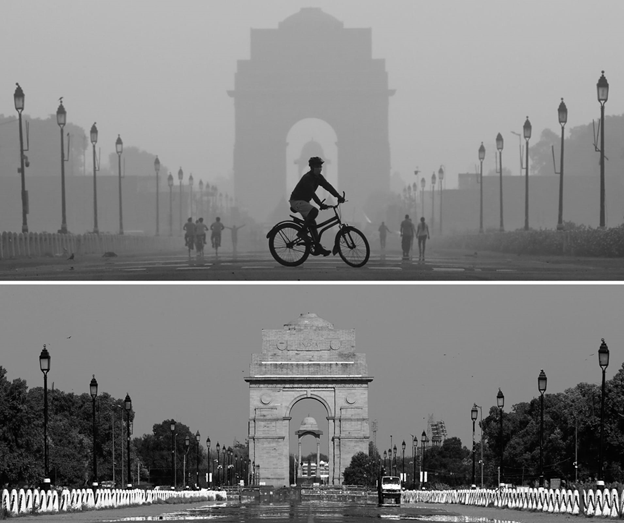
\includegraphics[width=0.6\linewidth]{images/air_pollution_greyscale} 

}

\caption{The India Gate in New Delhi, India.}\label{fig:covid}
\end{figure}

\vspace{.05in}

\begin{center}\includegraphics[width=0.6\linewidth]{10-paired_files/figure-latex/unnamed-chunk-2-1} \end{center}

\vspace{.2in}

\begin{longtable}[]{@{}ccll@{}}
\caption{Summary statistics for current AQI scores, median AQI scores from 2015--2019, and the differences in AQI scores.}\tabularnewline
\toprule
& Mean & Standard deviation & Sample size\tabularnewline
\midrule
\endfirsthead
\toprule
& Mean & Standard deviation & Sample size\tabularnewline
\midrule
\endhead
Current & \(\bar{x}_1\) = 47.394 & \(s_1\) = 14.107 & \(n_1\) = 33\tabularnewline
5 Year Median & \(\bar{x}_2\) = 51.545 & \(s_2\) = 17.447 & \(n_2\) = 33\tabularnewline
Differences & \(\bar{x}_d\) = -4.152 & \(s_d\) = 17.096 & \(n_d\) = 33\tabularnewline
\bottomrule
\end{longtable}

\newpage

\hypertarget{vocabulary-review.-complete-q1q5-before-class.}{%
\subsubsection*{Vocabulary review. Complete Q1--Q5 before class.}\label{vocabulary-review.-complete-q1q5-before-class.}}
\addcontentsline{toc}{subsubsection}{Vocabulary review. Complete Q1--Q5 before class.}

\begin{enumerate}
\def\labelenumi{\arabic{enumi}.}
\tightlist
\item
  What is the sample size?
\end{enumerate}

\vspace{0.5in}

\begin{enumerate}
\def\labelenumi{\arabic{enumi}.}
\setcounter{enumi}{1}
\tightlist
\item
  Identify the variables in this study. What role do each have?
\end{enumerate}

\vspace{.8in}

\begin{enumerate}
\def\labelenumi{\arabic{enumi}.}
\setcounter{enumi}{2}
\tightlist
\item
  Why is this treated as a paired study design and not two independent samples?
\end{enumerate}

\vspace{1in}

\begin{enumerate}
\def\labelenumi{\arabic{enumi}.}
\setcounter{enumi}{3}
\tightlist
\item
  Is this an experiment or observational study? Justify your answer.
\end{enumerate}

\vspace{0.3in}

\begin{enumerate}
\def\labelenumi{\arabic{enumi}.}
\setcounter{enumi}{4}
\tightlist
\item
  Are the differences in AQI scores independent for each case (US city)? Explain.
\end{enumerate}

\vspace{0.3in}

\hypertarget{ask-a-research-question}{%
\subsubsection*{Ask a research question}\label{ask-a-research-question}}
\addcontentsline{toc}{subsubsection}{Ask a research question}

\begin{enumerate}
\def\labelenumi{\arabic{enumi}.}
\setcounter{enumi}{5}
\tightlist
\item
  What are the two competing possibilities to run a hypothesis test for this study?
\end{enumerate}

\vspace{1in}

\begin{enumerate}
\def\labelenumi{\arabic{enumi}.}
\setcounter{enumi}{6}
\tightlist
\item
  Write the null hypothesis in words.
\end{enumerate}

\vspace{1in}

\begin{enumerate}
\def\labelenumi{\arabic{enumi}.}
\setcounter{enumi}{7}
\tightlist
\item
  What is the research question?
\end{enumerate}

\vspace{1in}

\begin{enumerate}
\def\labelenumi{\arabic{enumi}.}
\setcounter{enumi}{8}
\tightlist
\item
  Write the alternative hypothesis in notation.
\end{enumerate}

\vspace{1in}

\hypertarget{summarize-and-visualize-the-data}{%
\subsubsection*{Summarize and visualize the data}\label{summarize-and-visualize-the-data}}
\addcontentsline{toc}{subsubsection}{Summarize and visualize the data}

\begin{enumerate}
\def\labelenumi{\arabic{enumi}.}
\setcounter{enumi}{9}
\tightlist
\item
  Report the summary statistic for the data.
\end{enumerate}

\vspace{0.3in}

\begin{enumerate}
\def\labelenumi{\arabic{enumi}.}
\setcounter{enumi}{10}
\tightlist
\item
  What notation is used for the value in question 10?
\end{enumerate}

\vspace{0.3in}

\hypertarget{use-statistical-inferential-methods-to-draw-inferences-from-the-data}{%
\subsubsection*{Use statistical inferential methods to draw inferences from the data}\label{use-statistical-inferential-methods-to-draw-inferences-from-the-data}}
\addcontentsline{toc}{subsubsection}{Use statistical inferential methods to draw inferences from the data}

To simulate the null distribution we will use a bootstrapping method. Recall that the null distribution must be created under the assumption that the null hypothesis is true. Therefore, before bootstrapping we will need to shift each data point by the difference \(\mu_0 - \bar{x}\). This will ensure that the mean of the shifted data is \(\mu_0\) and that the simulated null distribution will be centered at the null value.

\begin{enumerate}
\def\labelenumi{\arabic{enumi}.}
\setcounter{enumi}{11}
\tightlist
\item
  Calculate the difference \(\mu_0 - \bar{x}\). Will we need to shift the data up or down?
\end{enumerate}

\vspace{.7in}

\begin{enumerate}
\def\labelenumi{\arabic{enumi}.}
\setcounter{enumi}{12}
\tightlist
\item
  Use the provided \texttt{R} script file and enter the calculated value from question 12 for xx to simulate the null distribution and enter the summary statistic from question 10 for yy to find the p-value. Highlight and run lines 1--21.
\end{enumerate}

\begin{Shaded}
\begin{Highlighting}[]
    \KeywordTok{paired_test}\NormalTok{(}\DataTypeTok{data =}\NormalTok{ Air}\OperatorTok{$}\NormalTok{Difference,   }\CommentTok{# Vector of differences or data set with column for each group}
            \DataTypeTok{shift =}\NormalTok{ xx,   }\CommentTok{# Shift needed for bootstrap hypothesis test}
            \DataTypeTok{as_extreme_as =}\NormalTok{ yy,  }\CommentTok{# Observed statistic}
            \DataTypeTok{direction =} \StringTok{"less"}\NormalTok{,  }\CommentTok{# Direction of alternative}
            \DataTypeTok{number_repetitions =} \DecValTok{1000}\NormalTok{,  }\CommentTok{# Number of simulated samples for null distribution}
            \DataTypeTok{which_first =} \DecValTok{1}\NormalTok{)  }\CommentTok{# Not needed when using calculated differences}
\end{Highlighting}
\end{Shaded}

\begin{enumerate}
\def\labelenumi{\arabic{enumi}.}
\setcounter{enumi}{13}
\tightlist
\item
  Sketch the null distribution created in question 13 here.
\end{enumerate}

\vspace{2in}

\begin{enumerate}
\def\labelenumi{\arabic{enumi}.}
\setcounter{enumi}{14}
\tightlist
\item
  Explain why the null distribution is centered at zero.
\end{enumerate}

\vspace{.5in}

\begin{enumerate}
\def\labelenumi{\arabic{enumi}.}
\setcounter{enumi}{15}
\tightlist
\item
  What proportion of samples are at or less than the sample mean difference in AQI scores for current scores minus 5 year median scores?
\end{enumerate}

\vspace{.3in}

\begin{enumerate}
\def\labelenumi{\arabic{enumi}.}
\setcounter{enumi}{16}
\tightlist
\item
  Interpret the p-value in the context of the problem.
\end{enumerate}

\vspace{.8in}

\begin{enumerate}
\def\labelenumi{\arabic{enumi}.}
\setcounter{enumi}{17}
\tightlist
\item
  How much evidence does this provide for improved air quality in U.S. cities?
\end{enumerate}

\vspace{.3in}

\begin{enumerate}
\def\labelenumi{\arabic{enumi}.}
\setcounter{enumi}{18}
\tightlist
\item
  Write out the parameter of interest in context of the study.
\end{enumerate}

\vspace{.6in}

\begin{enumerate}
\def\labelenumi{\arabic{enumi}.}
\setcounter{enumi}{19}
\tightlist
\item
  Using the provided \texttt{R} script file fill in the missing value at xx in the paired bootstrap CI to find a 99\% confidence interval, highlight and run lines 24--27. Report the confidence interval in interval notation.
\end{enumerate}

\begin{Shaded}
\begin{Highlighting}[]
\KeywordTok{paired_bootstrap_CI}\NormalTok{(}\DataTypeTok{data =}\NormalTok{ Air}\OperatorTok{$}\NormalTok{Difference, }\CommentTok{# Enter vector of differences}
                    \DataTypeTok{number_repetitions =} \DecValTok{1000}\NormalTok{, }\CommentTok{# Number of bootstrap samples for CI}
                    \DataTypeTok{confidence_level =}\NormalTok{ xx,  }\CommentTok{# Confidence level in decimal form}
                    \DataTypeTok{which_first =} \DecValTok{1}\NormalTok{)  }\CommentTok{# Not needed when entering vector of differences}
\end{Highlighting}
\end{Shaded}

\vspace{.3in}

\hypertarget{communicate-the-results-and-answer-the-research-question.}{%
\subsubsection*{Communicate the results and answer the research question.}\label{communicate-the-results-and-answer-the-research-question.}}
\addcontentsline{toc}{subsubsection}{Communicate the results and answer the research question.}

\begin{enumerate}
\def\labelenumi{\arabic{enumi}.}
\setcounter{enumi}{20}
\tightlist
\item
  Interpret the 99\% confidence interval in the context of the problem.
\end{enumerate}

\vspace{.8in}

\begin{enumerate}
\def\labelenumi{\arabic{enumi}.}
\setcounter{enumi}{21}
\tightlist
\item
  Do the results of your confidence interval and hypothesis test agree? What does each tell you about the null hypothesis?
\end{enumerate}

\vspace{.7in}

\begin{enumerate}
\def\labelenumi{\arabic{enumi}.}
\setcounter{enumi}{22}
\tightlist
\item
  Write a paragraph summarizes the results of this study as if you were describing the results to your roommate. Be sure to describe:
\end{enumerate}

\begin{itemize}
\item
  Summary statistic
\item
  P-value and interpretation
\item
  Conclusion (written to answer the research question)
\item
  Confidence interval and interpretation
\item
  Scope of inference
\end{itemize}

\vspace{3in}

\hypertarget{revisit-and-look-forward}{%
\subsubsection*{Revisit and look forward}\label{revisit-and-look-forward}}
\addcontentsline{toc}{subsubsection}{Revisit and look forward}

\begin{enumerate}
\def\labelenumi{\arabic{enumi}.}
\setcounter{enumi}{23}
\tightlist
\item
  Would it be possible to design an experiment to determine if the changed human behavior due to the COVID-19 pandemic causes a decrease in air pollution? Explain.
  \vspace{0.6in}
\end{enumerate}

\hypertarget{out-of-class-activity}{%
\subsection{Out-of-class activity}\label{out-of-class-activity}}

The remaining questions cover theory-based methods for testing paired quantitative data. Use section 6.2.3 in the textbook and the OneMeanTheory video to complete the following questions.

The sampling distribution for \(\bar{x}\) based on a sample of size \(n\) from a population with a true mean \(\mu\) and true standard deviation \(\sigma\) can be modeled using a normal distribution when certain conditions are met.

Conditions for the sample distribution of \(\bar{x}\).

\begin{itemize}
\item
  Independence: The sample's observations are independent
\item
  Normality: data should be approximately normal

  \begin{itemize}
  \item
    n \(<\) 30: If the sample size n is less than 30 and there are no clear outliers in the data, then we typically assume the data come from a nearly normal distribution to satisfy the condition.
  \item
    n \(\geq\) 30: If the sample size n is at least 30 and there are no particularly extreme outliers, then we typically assume the sampling distribution of \(\bar{x}\) is nearly normal, even if the underlying distribution of individual observations is not.
  \end{itemize}
\end{itemize}

\begin{enumerate}
\def\labelenumi{\arabic{enumi}.}
\tightlist
\item
  In the in-class activity we verified that the independence condition was satisfied. Is the normality condition met to use the theory-based methods for analysis? Explain your answer.
\end{enumerate}

\vspace{1in}

To find the standardized statistic for the paired differences we will use the following formula:

\[T = \frac{\bar{x}_d}{SE(\bar{x}_d)}\]

where the standard error of the mean difference is:

\[SE(\bar{x}_d)=\frac{s_d}{\sqrt{n}}\]

\begin{enumerate}
\def\labelenumi{\arabic{enumi}.}
\setcounter{enumi}{1}
\tightlist
\item
  Calculate the standard error of the mean difference.
\end{enumerate}

\vspace{0.5in}

\begin{enumerate}
\def\labelenumi{\arabic{enumi}.}
\setcounter{enumi}{2}
\tightlist
\item
  Calculate the standardized statistic.
\end{enumerate}

\vspace{0.5in}

Using the provided \texttt{R} script file, enter the T score (for xx) into the pt function using a df = minimum(n - 1) = 33 - 1 = 32, and lower.tail = TRUE to find the p-value. Highlight and run line 31.

\begin{Shaded}
\begin{Highlighting}[]
\KeywordTok{pt}\NormalTok{(xx, }\DataTypeTok{df=}\DecValTok{32}\NormalTok{, }\DataTypeTok{lower.tail=}\OtherTok{TRUE}\NormalTok{)}
\end{Highlighting}
\end{Shaded}

\begin{enumerate}
\def\labelenumi{\arabic{enumi}.}
\setcounter{enumi}{3}
\tightlist
\item
  Is the p-value found using theory-based methods similar to the simulation p-value found in the in-class activity?
\end{enumerate}

\vspace{0.5in}

To calculate the 99\% confidence interval use the following formula:

\[\bar{x}_d\pm t^* SE(\bar{x}_d)\]

We will need to find the \(t^*\) multiplier using the function qt. For a 99\% confidence interval we are finding the \(t^*\) value at the 99.5th percentile with df = n - 1 = 33 - 1 = 32.

\begin{Shaded}
\begin{Highlighting}[]
\KeywordTok{qt}\NormalTok{(}\FloatTok{0.995}\NormalTok{, }\DataTypeTok{df =} \DecValTok{32}\NormalTok{, }\DataTypeTok{lower.tail=}\OtherTok{TRUE}\NormalTok{)}
\CommentTok{#> [1] 2.738481}
\end{Highlighting}
\end{Shaded}

\begin{enumerate}
\def\labelenumi{\arabic{enumi}.}
\setcounter{enumi}{4}
\tightlist
\item
  Calculate the 99\% confidence interval using theory-based methods.
\end{enumerate}

\vspace{1in}

\begin{enumerate}
\def\labelenumi{\arabic{enumi}.}
\setcounter{enumi}{5}
\tightlist
\item
  Explain why the theory-based and simulation confidence intervals are not quite the same.
\end{enumerate}

\vspace{1in}

\hypertarget{take-home-messages}{%
\subsection{Take-home messages}\label{take-home-messages}}

\begin{enumerate}
\def\labelenumi{\arabic{enumi}.}
\item
  The differences in a paired data set is treated like a single quantitative variable when analyzing. Paired data (or paired samples) occur when pairs of measurements are collected. We are only interested in the population (and sample) of differences, and not in the original data.
\item
  When using bootstrapping to create the null distribution centered at the null value for both paired data and a single quantitative variable we first need to shift the data by the difference, \(\mu_0 - \bar{x}_d\) and then sample with replacement from the shifted data.
\item
  When analyzing paired data the summary statistic is the mean difference NOT the difference in means. This terminology will be \emph{very} important in the interpretations.
\end{enumerate}

\hypertarget{additional-notes}{%
\subsection{Additional notes}\label{additional-notes}}

Use this space to summarize your thoughts and take additional notes on today's activity.

\hypertarget{inference-for-a-quantitative-response-with-independent-samples}{%
\chapter{Inference for a Quantitative Response with Independent Samples}\label{inference-for-a-quantitative-response-with-independent-samples}}

\hypertarget{reading-guide-inference-for-a-difference-in-two-means}{%
\section{Reading Guide: Inference for a Difference in Two Means}\label{reading-guide-inference-for-a-difference-in-two-means}}

\hypertarget{section-6.3-inference-for-a-difference-in-two-means}{%
\subsection*{Section 6.3 (Inference for a difference in two means)}\label{section-6.3-inference-for-a-difference-in-two-means}}
\addcontentsline{toc}{subsection}{Section 6.3 (Inference for a difference in two means)}

\textbf{Videos}

\begin{itemize}
\tightlist
\item
  6.3
\item
  TwoMeanRand
\end{itemize}

\setstretch{1.25}

\hypertarget{reminders-from-previous-sections}{%
\subsubsection*{Reminders from previous sections}\label{reminders-from-previous-sections}}
\addcontentsline{toc}{subsubsection}{Reminders from previous sections}

\(n_1\)= sample size of group 1

\(n_2\) = sample size of group 2

\(\overline{x}\) = sample mean

\(s\) = sample standard deviation

\(\mu\) = population mean

\(\sigma\) = population standard deviation

General steps of a hypothesis test:

\begin{enumerate}
\def\labelenumi{\arabic{enumi}.}
\item
  Frame the research question in terms of hypotheses.
\item
  Collect and summarize data using a test statistic.
\item
  Assume the null hypothesis is true, and simulate or mathematically model a null distribution for the test statistic.
\item
  Compare the observed test statistic to the null distribution to calculate a p-value.
\item
  Make a conclusion based on the p-value and write the conclusion in context.
\end{enumerate}

Parameter: a value summarizing a variable(s) for a population

Statistic: a value summarizing a variable(s) for a sample

Sampling distribution: plot of statistics from 1000s of samples of the same size taken from the same population.

Standard deviation of a statistic: the variability of statistics from 1000s of samples. How far, on average, each statistic is from the true value of the parameter.

Standard error of a statistic: estimated standard deviation of a statistic.

Hypothesis test: a process to determine how strong the evidence of an effect is

\rgi Also called a `significance test'

Simulation-based method: Simulate lots of samples of size n, then find the proportion of the simulations that are at least as extreme as the observed sample statistic

Theory-based method: Develop a mathematical model for the statistic and use the model to calculate the probability of the observed sample statistic occurring

Null hypothesis: \(H_0\) the skeptical perspective; no difference; no change; no effect; random chance; what the researcher hopes to prove is \textbf{wrong}

Alternative hypothesis: \(H_A\) the new perspective; a difference/increase/decrease; an effect; not random chance; what the researcher hopes to prove is \textbf{correct}

Null value: the value of the parameter when we assume the null hypothesis is true (labeled as \(parameter_0\))

Null distribution: the simulated or modeled distribution of statistics (sampling distribution) we would expect to occur if the null hypothesis is true.

P-value: probability of seeing the observed sample data, or something more extreme, assuming the null hypothesis is true

\rgi Lower the p-value the stronger the evidence AGAINST the null hypothesis and FOR the alternative hypothesis

Decision: a determination of whether to reject or fail to reject a null hypothesis based on a p-value and a pre-set level of significance

Significance level: (\(\alpha\)) a threshold used to determine if a p-value provides enough evidence to reject the null hypothesis or not

\rgi Typically use \(\alpha\) =0.05

Statistically significant: results are considered statistically significant if the p-value is below the significance level.

Confidence interval: a process to determine how large an effect is; a range of plausible values for the parameter
\rgi Also called `estimation'

Margin of error: the value that is added to and subtracted from the sample statistic to create a confidence interval; half the width of a confidence interval

Bootstrapping: the process of drawing with replacement n times from the original sample

Bootstrapped resample: a random sample of size n from the original sample, selected with replacement

Bootstrapped statistic: the statistic recorded from the bootstrapped resample

Confidence level: how confident we are that the confidence interval will capture the parameter

Bootstrap X\% confidence interval: (\((\frac{(1-X)}{2})^{th}\) percentile,\((X+(\frac{(1-X)}{2})^{th}\) percentile) of a bootstrap distribution

Central Limit Theorem: For large sample sizes, the sampling distribution of a sample proportion (or mean) will be bell-shaped and symmetric

t-distribution: A bell-shaped symmetric distribution, centered at 0, wider than the standard Normal distribution
Note: width depends on the sample size (used to calculate degrees of freedom -- df for short)
Larger df  Closer the t distribution is to the standard Normal distribution

Degrees of freedom (df): describes the variability of the t-distribution

T-score: the name for a standardized statistic which is compared to a t-distribution

\hypertarget{notes}{%
\subsubsection*{Notes}\label{notes}}
\addcontentsline{toc}{subsubsection}{Notes}

To create a \textbf{simulated null distribution},

\begin{enumerate}
\def\labelenumi{\arabic{enumi}.}
\item
  How many cards will you need and how will the cards be labeled?
  \rgs
\item
  What do you do with the cards after labeling them?
  \rgs
\item
  After shuffling, what value will be plotted on the simulated null distribution?
  \rgs
\end{enumerate}

To create a \textbf{bootstrap distribution},

\begin{enumerate}
\def\labelenumi{\arabic{enumi}.}
\item
  How many cards will you need and how will the cards be labeled?
  \rgs
\item
  What do you do with the cards after labeling them?
  \rgs
\item
  After shuffling, what value will be plotted on the bootstrap distribution?
  \rgs
\end{enumerate}

Conditions to use the CLT for a difference in two means:
1. Independence:
\rgs

\rgi a. Checked by:
\rgs

\begin{enumerate}
\def\labelenumi{\arabic{enumi}.}
\setcounter{enumi}{1}
\tightlist
\item
  Normality:
  \rgs
\end{enumerate}

\rgi a. Checked by:
\rgs

In a two-sample t-test, how are the degrees of freedom determined?
\rgs		

True or False: A large p-value indicates that the null hypothesis is true.
\rgs

\hypertarget{formulas}{%
\subsubsection*{Formulas}\label{formulas}}
\addcontentsline{toc}{subsubsection}{Formulas}

\(SE(\overline{x_1} - \overline{x_2})=\)
\rgs

\(t=\)
\rgs

Confidence interval:
\rgs

\hypertarget{notation}{%
\subsubsection*{Notation}\label{notation}}
\addcontentsline{toc}{subsubsection}{Notation}

\(mu_1\) represents
\rgs

\(\mu_2\) represents
\rgs

\(\sigma_1\) represents
\rgs

\(\sigma_2\) represents
\rgs

\(\overline{x_1}\) represents
\rgs

\(\overline{x_2}\) represents
\rgs

\(s_1\) represents
\rgs

\(s_2\) represents
\rgs

\hypertarget{example-test-scores}{%
\subsubsection*{Example: Test scores}\label{example-test-scores}}
\addcontentsline{toc}{subsubsection}{Example: Test scores}

\begin{enumerate}
\def\labelenumi{\arabic{enumi}.}
\item
  What are the observational units?
  \rgs
\item
  What are the sample statistics presented in this example? What notation would be used to represent each value?
  \rgs
\item
  What is the parameter representing in the context of this problem? What notation would be used to represent this parameter?
  \rgs
  \rgs
\item
  What is the research question?
  \rgs
\item
  Write the null and alternative hypothesis in appropriate notation.
  \rgs
\item
  How could we use cards to simulate \textbf{1} sample \emph{which assumes the null hypothesis is true}? How many cards? What is written on the cards? What would we do with the cards? What would you record once you have a simulated sample?
  \rgs
  \rgs
\item
  After 1000 shuffles are generated, where is the resulting simulated distribution centered? Why does that make sense?
  \rgs
  \rgs
\item
  How was the p-value for this test found?
\end{enumerate}

The proportion of simulated null samples at \_\_\_\_ or \_\_\_\_\_\_\_\_\_\_\_.
\rgs

\begin{enumerate}
\def\labelenumi{\arabic{enumi}.}
\setcounter{enumi}{8}
\item
  Interpret the p-value in the context of the problem.
  \rgs
  \rgs
\item
  From these data, can we conclude the exams are equally difficult?
  \rgs
\item
  What type of error may have occurred at the 5\% significance level? Interpret that error in context.
  \rgs
  \rgs
\end{enumerate}

\hypertarget{example-esc-and-heart-attacks}{%
\subsubsection*{Example: ESC and heart attacks}\label{example-esc-and-heart-attacks}}
\addcontentsline{toc}{subsubsection}{Example: ESC and heart attacks}

\begin{enumerate}
\def\labelenumi{\arabic{enumi}.}
\item
  What is the research question?
  \rgs
\item
  What are the observational units?
  \rgs
\item
  What variables are recorded? Give the type and role of each.
  \rgs
  \rgs
\item
  What are the sample statistics presented in this example? What notation would be used to represent each value?
  \rgs
\item
  What is the parameter representing in the context of this problem? What notation would be used to represent this parameter?
  \rgs
  \rgs
\item
  How could we use cards to simulate \textbf{1} bootstrap resample \emph{which does not assume the null hypothesis is true}? How many cards? What is written on the cards? What would we do with the cards? What would you record once you have a simulated sample?
  \rgs
  \rgs
\item
  After 1000 resamples are generated, where is the resulting bootstrap distribution centered? Why does that make sense?
  \rgs
  \rgs
\item
  Does the 90\% confidence interval show that there is a difference across the two treatments?
  \rgs
  \rgs
\end{enumerate}

\hypertarget{example-nc-births}{%
\subsubsection*{Example: NC births}\label{example-nc-births}}
\addcontentsline{toc}{subsubsection}{Example: NC births}

\begin{enumerate}
\def\labelenumi{\arabic{enumi}.}
\item
  What is the research question?
  \rgs
\item
  What are the observational units?
  \rgs
\item
  What variables will be analyzed? Give the type and role of each.
  \rgs
  \rgs
\item
  Can the results of this study be generalized to a larger population?
  \rgs
\item
  Is causal inference appropriate for these data?
  \rgs
\item
  Write the null and the alternative hypothesis in words.
  \rgs
  \rgs
\item
  Write the null and the alternative hypothesis in notation.
  \rgs
\item
  What are the sample statistics presented in this example? What notation would be used to represent each value?
  \rgs
\item
  Are the independence and normality conditions satisfied?
  \rgs
  \rgs
\item
  Calculate the standard error of the difference in sample means.
  \rgs
\item
  Calculate the t-score (the standardized statistic for the sample mean).
  \rgs
\item
  What distribution should the t-score be compared to in order to calculate a p-value?
  \rgs
\item
  What was the p-value of the test?
  \rgs
\item
  What conclusion should the researcher make?
  \rgs
\item
  Calculate a 95\% confidence interval for the parameter of interest using \texttt{qt(0.975,\ df\ =\ 49)\ =\ 1.677} as the \(t^\star\) value.
  \rgs
\item
  Interpret your interval in the context of the problem.
  \rgs
  \rgs
\end{enumerate}

\newpage

\hypertarget{activity-weather-patterns-and-record-snowfall}{%
\section{Activity: Weather Patterns and Record Snowfall}\label{activity-weather-patterns-and-record-snowfall}}

\setstretch{1}

\hypertarget{learning-objectives}{%
\subsection{Learning objectives}\label{learning-objectives}}

\begin{itemize}
\item
  Given a research question involving one categorical explanatory variable and one quantitative response variable, construct the null and alternative hypotheses
  in words and using appropriate statistical symbols.
\item
  Describe and perform a simulation-based hypothesis test for a difference in means.
\item
  Interpret and evaluate a p-value for a simulation-based hypothesis test for a difference in means.
\item
  Use bootstrapping to find a confidence interval for a difference in means.
\item
  Interpret a confidence interval for a difference in means.
\item
  Use a confidence interval to determine the conclusion of a hypothesis test.
\end{itemize}

\hypertarget{terminology-review}{%
\subsection{Terminology review}\label{terminology-review}}

In this week's in-class activity, we will use simulation-based methods to analyze one categorical and one quantitative variable, where the groups formed by the categorical variable are independent. Some terms covered in this activity are:

\begin{itemize}
\item
  Independent groups
\item
  Difference in means
\end{itemize}

To review these concepts, see Section 6.3 in the textbook.

\hypertarget{weather-patterns-and-record-snowfall}{%
\subsection{Weather patterns and record snowfall}\label{weather-patterns-and-record-snowfall}}

In the winter of 2018-2019, Bozeman had a record snowfall which resulted in the collapse of two flat-roofed buildings on the MSU campus. A writer for the Washington Post predicted the heavy snowfall for 2018-2019 due to the El Ni\latexcode{\~{n}}o weather pattern that occurred in that season. A meteorologist in Montana wanted to see if the weather pattern really was associated with total snowfall. She obtained historical data from 44 years on the weather pattern (El Ni\latexcode{\~{n}}o or La Ni\latexcode{\~{n}}a) and snowfall (in inches) at the Billings Weather Station.

Notice from the \texttt{R} code that the name of the data set is \texttt{Snow}.

\begin{Shaded}
\begin{Highlighting}[]
\NormalTok{Snow <-}\StringTok{ }\KeywordTok{read.csv}\NormalTok{(}\StringTok{"data/SnowfallbyWeatherPattern.csv"}\NormalTok{) }\CommentTok{# Read in data set}
\CommentTok{# Code categorical variables as factors}
\NormalTok{Snow <-}\StringTok{ }\CommentTok{# Write over original data with the following}
\StringTok{  }\NormalTok{Snow }\OperatorTok\StringTok{ }\CommentTok{# Pipe data set into}
\StringTok{  }\KeywordTok{mutate}\NormalTok{(}\DataTypeTok{WeatherPattern =} \KeywordTok{factor}\NormalTok{(WeatherPattern)) }\CommentTok{# Convert to factor}
\end{Highlighting}
\end{Shaded}

\newpage

\begin{Shaded}
\begin{Highlighting}[]
\CommentTok{# Side-by-side box plots}
\NormalTok{Snow }\OperatorTok
\KeywordTok{ggplot}\NormalTok{(}\KeywordTok{aes}\NormalTok{(}\DataTypeTok{x =}\NormalTok{ WeatherPattern, }\DataTypeTok{y =}\NormalTok{ Snowfall)) }\OperatorTok{+}
\StringTok{    }\KeywordTok{geom_boxplot}\NormalTok{() }\OperatorTok{+}\StringTok{ }
\StringTok{    }\KeywordTok{labs}\NormalTok{(}\DataTypeTok{title =} \StringTok{"Snowfall by weather pattern"}\NormalTok{,}
         \DataTypeTok{x =} \StringTok{"Weather pattern"}\NormalTok{) }\OperatorTok{+}
\StringTok{    }\KeywordTok{coord_flip}\NormalTok{()}
\end{Highlighting}
\end{Shaded}

\begin{center}\includegraphics[width=0.6\linewidth]{11-inference-1ofeach_files/figure-latex/unnamed-chunk-2-1} \end{center}

\begin{Shaded}
\begin{Highlighting}[]
\CommentTok{# Summary statistics}
\NormalTok{Snow }\OperatorTok\StringTok{ }
\StringTok{     }\KeywordTok{summarize}\NormalTok{(}\KeywordTok{favstats}\NormalTok{(Snowfall}\OperatorTok{~}\NormalTok{WeatherPattern))}
\end{Highlighting}
\end{Shaded}

\begin{verbatim}
#>   WeatherPattern  min   Q1 median   Q3   max     mean       sd  n missing
#> 1        El_Nino 31.9 46.4   57.7 64.3  87.9 56.23043 13.00823 23       0
#> 2        La_Nina 44.5 51.4   60.9 70.3 107.2 63.13333 15.48626 21       0
\end{verbatim}

\hypertarget{quantitative-variables-review.-complete-q1q5-before-class.}{%
\subsubsection*{Quantitative variables review. Complete Q1--Q5 before class.}\label{quantitative-variables-review.-complete-q1q5-before-class.}}
\addcontentsline{toc}{subsubsection}{Quantitative variables review. Complete Q1--Q5 before class.}

\begin{enumerate}
\def\labelenumi{\arabic{enumi}.}
\tightlist
\item
  The two variables assessed in this study are the type of weather pattern and snowfall. Identify the role for each variable (explanatory, response).
\end{enumerate}

\vspace{.6in}

\begin{enumerate}
\def\labelenumi{\arabic{enumi}.}
\setcounter{enumi}{1}
\tightlist
\item
  Which group (El Ni\latexcode{\~{n}}o or La Ni\latexcode{\~{n}}a) has the highest center? Explain which measure of center you are using.
\end{enumerate}

\vspace{.6in}

\begin{enumerate}
\def\labelenumi{\arabic{enumi}.}
\setcounter{enumi}{2}
\tightlist
\item
  Using the side-by-side boxplots, which group has the largest spread? How did you make that choice?
\end{enumerate}

\vspace{.6in}

\newpage

\begin{enumerate}
\def\labelenumi{\arabic{enumi}.}
\setcounter{enumi}{3}
\tightlist
\item
  Is this an experiment or an observational study? Justify your answer.
\end{enumerate}

\vspace{1in}

\begin{enumerate}
\def\labelenumi{\arabic{enumi}.}
\setcounter{enumi}{4}
\tightlist
\item
  Is this a paired data set or two independent groups? Explain your reasoning.
\end{enumerate}

\vspace{1in}

\hypertarget{ask-a-research-question}{%
\subsubsection*{Ask a research question}\label{ask-a-research-question}}
\addcontentsline{toc}{subsubsection}{Ask a research question}

\begin{enumerate}
\def\labelenumi{\arabic{enumi}.}
\setcounter{enumi}{5}
\tightlist
\item
  Write out the parameter of interest in context of the study. Use proper notation and be sure to define your subscripts. Use El Ni\latexcode{\~{n}}o minus La Ni\latexcode{\~{n}}a as the order of subtraction.
\end{enumerate}

\vspace{1in}

\begin{enumerate}
\def\labelenumi{\arabic{enumi}.}
\setcounter{enumi}{6}
\tightlist
\item
  What are the two competing possibilities we will evaluate in this study?
\end{enumerate}

\vspace{1in}

\begin{enumerate}
\def\labelenumi{\arabic{enumi}.}
\setcounter{enumi}{7}
\tightlist
\item
  Identify which of your answers in question 7 is the null hypothesis and which is the alternative hypothesis.
\end{enumerate}

\vspace{1in}

\hypertarget{summarize-and-visualize-the-data}{%
\subsubsection*{Summarize and visualize the data}\label{summarize-and-visualize-the-data}}
\addcontentsline{toc}{subsubsection}{Summarize and visualize the data}

\begin{enumerate}
\def\labelenumi{\arabic{enumi}.}
\setcounter{enumi}{8}
\tightlist
\item
  Calculate the summary statistic. Use El Ni\latexcode{\~{n}}o minus La Ni\latexcode{\~{n}}a as the order of subtraction. What is the appropriate notation for the statistic?
\end{enumerate}

\vspace{0.5in}

\newpage

\hypertarget{use-statistical-inferential-methods-to-draw-inferences-from-the-data}{%
\subsubsection*{Use statistical inferential methods to draw inferences from the data}\label{use-statistical-inferential-methods-to-draw-inferences-from-the-data}}
\addcontentsline{toc}{subsubsection}{Use statistical inferential methods to draw inferences from the data}

Remember that the null distribution is created based on the assumption the null hypothesis is true. In this study, we assume there is no association between variables. This means that a snowfall value could be in either an El Ni\latexcode{\~{n}}o year or a La Ni\latexcode{\~{n}}a year.

To demonstrate this your instructor will use cards to represent the sample.

\begin{enumerate}
\def\labelenumi{\arabic{enumi}.}
\setcounter{enumi}{9}
\tightlist
\item
  How many cards will we start with?
\end{enumerate}

\vspace{0.5in}

\begin{enumerate}
\def\labelenumi{\arabic{enumi}.}
\setcounter{enumi}{10}
\tightlist
\item
  What will we write on each card?
\end{enumerate}

\vspace{0.5in}

\begin{enumerate}
\def\labelenumi{\arabic{enumi}.}
\setcounter{enumi}{11}
\tightlist
\item
  Next we will mix the cards together and shuffle into two piles. How many cards will go into each pile? What should we label the piles?
\end{enumerate}

\vspace{1in}

\begin{enumerate}
\def\labelenumi{\arabic{enumi}.}
\setcounter{enumi}{12}
\tightlist
\item
  What value is calculated from the cards and plotted on the null distribution? \emph{Hint}: What statistic are we calculating from the data?
\end{enumerate}

\vspace{0.3in}

\begin{enumerate}
\def\labelenumi{\arabic{enumi}.}
\setcounter{enumi}{13}
\tightlist
\item
  Once we create a null distribution of 1000 simulations, at what value do you expect the distribution to be centered? Explain your reasoning.
\end{enumerate}

\vspace{.8in}

\textbf{Simulation method}

\begin{enumerate}
\def\labelenumi{\arabic{enumi}.}
\setcounter{enumi}{14}
\tightlist
\item
  When using the two mean test we need to enter the name of the response variable, \texttt{Snowfall} and the name of the explanatory variable, \texttt{WeatherPattern} for the formula. The name of the data set as shown above is \texttt{Snow}. What values should be entered for each of the following into the two mean test to create 1000 simulations?
\end{enumerate}

\vspace{.2in}

\begin{itemize}
\tightlist
\item
  First in Subtraction (What is the outcome for the explanatory variable that is used as first in the order of subtraction? \texttt{"El\_Nino"} or \texttt{"La\_Nina"}:
\end{itemize}

\vspace{.2in}

\begin{itemize}
\tightlist
\item
  Number of repetitions:
\end{itemize}

\vspace{.2in}

\begin{itemize}
\tightlist
\item
  As extreme as:
\end{itemize}

\vspace{.2in}

\begin{itemize}
\tightlist
\item
  Direction (\texttt{"greater"}, \texttt{"less"}, or \texttt{"two-sided"}):
\end{itemize}

\vspace{.2in}

\begin{enumerate}
\def\labelenumi{\arabic{enumi}.}
\setcounter{enumi}{15}
\tightlist
\item
  Using the \texttt{R} script file for this activity, enter your answers for question 15 in place of the xx's to produce the null distribution with 1000 simulations. Highlight and run lines 1--29.
\end{enumerate}

\begin{Shaded}
\begin{Highlighting}[]
\KeywordTok{two_mean_test}\NormalTok{(Snowfall}\OperatorTok{~}\NormalTok{WeatherPattern, }\DataTypeTok{data =}\NormalTok{ Snow,  }\CommentTok{# Variables and data}
                    \DataTypeTok{first_in_subtraction =} \StringTok{"xx"}\NormalTok{, }\CommentTok{# First outcome in order of subtraction}
                    \DataTypeTok{number_repetitions =} \DecValTok{1000}\NormalTok{,  }\CommentTok{# Number of simulations}
                    \DataTypeTok{as_extreme_as =}\NormalTok{ xx,  }\CommentTok{# Observed statistic}
                    \DataTypeTok{direction =} \StringTok{"xx"}\NormalTok{)  }\CommentTok{# Direction of alternative: "greater", "less", or "two-sided"}
\end{Highlighting}
\end{Shaded}

Sketch the null distribution created using the code above.
\vspace{1.5in}

\begin{enumerate}
\def\labelenumi{\arabic{enumi}.}
\setcounter{enumi}{16}
\tightlist
\item
  Report the p-value. How much evidence does the p-value provide against the null hypothesis?
\end{enumerate}

\vspace{0.5in}

\begin{enumerate}
\def\labelenumi{\arabic{enumi}.}
\setcounter{enumi}{17}
\tightlist
\item
  Using bootstrapping find a 95\% confidence interval. Use the provided \texttt{R} script file for the two mean bootstrap CI function. Enter the variable names and data set name as in the two mean test, outcome name for the first in subtraction, number of repetitions, and the confidence level as a decimal. Highlight and run lines 32--35. Report the 95\% confidence interval in interval notation.
\end{enumerate}

\begin{Shaded}
\begin{Highlighting}[]
\KeywordTok{two_mean_bootstrap_CI}\NormalTok{(RESPONSE}\OperatorTok{~}\NormalTok{EXPLANATORY, }\DataTypeTok{data =}\NormalTok{ DATASET,  }\CommentTok{# Variables and data}
                      \DataTypeTok{first_in_subtraction =} \StringTok{"xx"}\NormalTok{, }\CommentTok{# First value in order of subtraction}
                      \DataTypeTok{number_repetitions =} \DecValTok{1000}\NormalTok{,  }\CommentTok{# Number of simulations}
                      \DataTypeTok{confidence_level =}\NormalTok{ xx)}
\end{Highlighting}
\end{Shaded}

\vspace{0.3in}

\begin{enumerate}
\def\labelenumi{\arabic{enumi}.}
\setcounter{enumi}{18}
\tightlist
\item
  Interpret the interval you calculated in question 18.
\end{enumerate}

\vspace{1in}

\hypertarget{communicate-the-results-and-answer-the-research-question}{%
\subsubsection*{Communicate the results and answer the research question}\label{communicate-the-results-and-answer-the-research-question}}
\addcontentsline{toc}{subsubsection}{Communicate the results and answer the research question}

\begin{enumerate}
\def\labelenumi{\arabic{enumi}.}
\setcounter{enumi}{19}
\tightlist
\item
  Write a paragraph summarizing the results of the study as if you are reporting the results to your supervisor. Be sure to describe:
\end{enumerate}

\begin{itemize}
\item
  Summary statistic
\item
  P-value and interpretation
\item
  Conclusion (written to answer the research question)
\item
  Confidence interval and interpretation
\item
  Scope of inference
\end{itemize}

\vspace{3in}

\hypertarget{revisit-and-look-forward}{%
\subsubsection*{Revisit and look forward}\label{revisit-and-look-forward}}
\addcontentsline{toc}{subsubsection}{Revisit and look forward}

\begin{enumerate}
\def\labelenumi{\arabic{enumi}.}
\setcounter{enumi}{20}
\tightlist
\item
  Would the results from the theory-based test match the results we saw with the simulation? Explain why or why not.
\end{enumerate}

\vspace{1in}

\begin{enumerate}
\def\labelenumi{\arabic{enumi}.}
\setcounter{enumi}{21}
\tightlist
\item
  If we had data on 45 La Ni\latexcode{\~{n}}a years and 47 El Ni\latexcode{\~{n}}o years and found a similar summary statistic, what would happen to the p-value? The width of the confidence interval? The power of the test?
\end{enumerate}

\vspace{1in}

\hypertarget{out-of-class-activity}{%
\subsection{Out-of-class activity}\label{out-of-class-activity}}

The remaining questions cover inference for a difference in means using theory based methods. Use section 6.3.3 in the textbook and the TwoMeanTheory video to complete the following questions.

The sampling distribution for \(\bar{x}_1-\bar{x}_2\) can be modeled using a normal distribution when certain conditions are met.

Conditions for the sample distribution of \(\bar{x}_1-\bar{x}_2\).

\begin{itemize}
\item
  Independence: The sample's observations are independent
\item
  Normality: each sample should be approximately normal

  \begin{itemize}
  \item
    For each sample:

    \begin{itemize}
    \item
      \(n < 30\): If the sample size n is less than 30 and there are no clear outliers in the data, then we typically assume the data come from a nearly normal distribution to satisfy the condition.
    \item
      \(n \le 30\): If the sample size n is at least 30 and there are no particularly extreme outliers, then we typically assume the sampling distribution of \(\bar{x}\) is nearly normal, even if the underlying distribution of individual observations is not.
    \end{itemize}
  \end{itemize}
\end{itemize}

\begin{enumerate}
\def\labelenumi{\arabic{enumi}.}
\tightlist
\item
  In question 21 in the in-class activity we noted that there were issues with the normality condition. Explain how that will affect the p-value and confidence interval found with theory-based methods.
\end{enumerate}

\vspace{1in}

To find the Standardized Statistic for the difference in means we will calculate:

\[T = \frac{\bar{x}_1-\bar{x}_2}{SE(\bar{x}_1-\bar{x}_2)}\]

where the standard error of the difference in means is calculated using:

\[SE(\bar{x}_1 -\bar{x}_2)=\sqrt{\frac{s_1^2}{n_1}+\frac{s_2^2}{n_2}}\]
\newpage

\begin{enumerate}
\def\labelenumi{\arabic{enumi}.}
\setcounter{enumi}{1}
\tightlist
\item
  Calculate the standard error of the difference in means.
\end{enumerate}

\vspace{0.5in}

\begin{enumerate}
\def\labelenumi{\arabic{enumi}.}
\setcounter{enumi}{2}
\tightlist
\item
  Calculate the standardized statistic for the difference in means.
\end{enumerate}

\vspace{0.5in}

Using the provided \texttt{R} script file, enter the T score (for xx) into the pt function using a df = minimum(n - 1) = 21 - 1 = 20, and lower.tail = TRUE to find the p-value. Highlight and run line 39.

\begin{Shaded}
\begin{Highlighting}[]
\DecValTok{2}\OperatorTok{*}\KeywordTok{pt}\NormalTok{(xx, }\DataTypeTok{df=}\DecValTok{20}\NormalTok{, }\DataTypeTok{lower.tail=}\OtherTok{TRUE}\NormalTok{)}
\end{Highlighting}
\end{Shaded}

\begin{enumerate}
\def\labelenumi{\arabic{enumi}.}
\setcounter{enumi}{3}
\tightlist
\item
  Explain why we multiplied by 2 in the code above.
\end{enumerate}

\vspace{0.3in}

\begin{enumerate}
\def\labelenumi{\arabic{enumi}.}
\setcounter{enumi}{4}
\tightlist
\item
  Report the p-value from the \texttt{R} output.
\end{enumerate}

\vspace{0.3in}

\begin{enumerate}
\def\labelenumi{\arabic{enumi}.}
\setcounter{enumi}{5}
\tightlist
\item
  Explain why the p-value found using theory-based methods from the p-value found using simulation methods in the in-class activity.
\end{enumerate}

\vspace{0.5in}

To calculate the 95\% confidence interval use the formula:

\[\bar{x}_1- \bar{x}_2\pm t^* SE(\bar{x}_1- \bar{x}_2)\]

We will need to find the \(t^*\) multiplier using the function qt. For a 95\% confidence interval we are finding the \(t^*\) value at the 97.5th percentile with df = minimum(n - 1) = 21 - 1 = 20.

\begin{verbatim}
#> [1] 2.085963
\end{verbatim}

\begin{enumerate}
\def\labelenumi{\arabic{enumi}.}
\setcounter{enumi}{6}
\tightlist
\item
  Calculate the 95\% confidence interval using theory-based methods.
\end{enumerate}

\vspace{1in}

\hypertarget{take-home-messages}{%
\subsection{Take-home messages}\label{take-home-messages}}

\begin{enumerate}
\def\labelenumi{\arabic{enumi}.}
\item
  This activity differs from Activity 10 because the responses are independent not paired. These data are analyzed as a difference in means.
\item
\end{enumerate}

\hypertarget{additional-notes}{%
\subsection{Additional notes}\label{additional-notes}}

Use this space to summarize your thoughts and take additional notes on today's activity.

\hypertarget{inference-for-two-quantitative-variables}{%
\chapter{Inference for Two Quantitative Variables}\label{inference-for-two-quantitative-variables}}

\hypertarget{reading-guide-inference-for-slope-and-correlation}{%
\section{Reading Guide: Inference for Slope and Correlation}\label{reading-guide-inference-for-slope-and-correlation}}

\hypertarget{sections-7.1-and-7.2-inference-for-regression-and-model-conditions}{%
\subsection*{Sections 7.1 and 7.2 (Inference for regression and model conditions)}\label{sections-7.1-and-7.2-inference-for-regression-and-model-conditions}}
\addcontentsline{toc}{subsection}{Sections 7.1 and 7.2 (Inference for regression and model conditions)}

\textbf{Videos}

\begin{itemize}
\tightlist
=======
>>>>>>> 6902ece40b9553d6adf5f64bb69bb844cf53bb72
\item
  What is the research question?
  \rgs
\item
<<<<<<< HEAD
  RegressionSim
\end{itemize}

\setstretch{1.25}

\hypertarget{reminders-from-previous-sections}{%
\subsubsection*{Reminders from previous sections}\label{reminders-from-previous-sections}}
\addcontentsline{toc}{subsubsection}{Reminders from previous sections}

\(\beta_0\): population y-intercept

\(\beta_1\): population slope

\(\rho\): population correlation

\(b_0\): sample y-intercept

\(b_1\): sample slope

\(r\): sample correlation

Scatterplot: displays two quantitative variables; one dot = two measurements (x, y) on one observational unit

Four characteristics of a scatterplot:

\rgi *Form*: pattern of the dots plotted. Is the trend generally linear (you can fit a straight line to the data) or non-linear?

\rgi *Strength*: how closely do the points follow a trend? Very closely (strong)? No pattern (weak)?

\rgi *Direction*: as the x values increase, do the y-values tend to increase (positive) or decrease (negative)?

\rgi *Unusual observations or outliers*: points that do not fit the overall pattern of the data

Least squares regression line: \(\hat{y} = b_0+b_1x\) , where \(b_0\) is the estimate for \texttt{(Intercept)} and \(b_1\) is the estimate for the \texttt{x-variable} name in the \texttt{R} regression output.

Slope interpretation: a 1 unit increase in the \emph{x} variable is associated with a \(|b_1 |\) unit increase/decrease in the \emph{y}-variable

General steps of a hypothesis test:

\begin{enumerate}
\def\labelenumi{\arabic{enumi}.}
=======
  What are the observational units?
  \rgs
\item
  What type of study design was used? Justify your answer.
  \rgs
\item
  What is the appropriate scope of inference for these data?
  \rgs
\item
  What is the sample difference in proportions presented in this example? What notation would be used to represent this value?
  \rgs
\item
  What is the sample relative risk? Interpret the value in the context of the study.
  \rgs
  \rgs
>>>>>>> 6902ece40b9553d6adf5f64bb69bb844cf53bb72
\item
  What is the parameter (using a difference in proportion) representing in the context of this problem? What notation would be used to represent this parameter?
  \rgs
  \rgs
\item
  Write the null and the alternative hypotheses in words.
  \rgs
  \rgs
\item
  Write the null and the alternative hypotheses in notation.
  \rgs
\item
  How could we use cards to simulate \textbf{1} sample \emph{which assumes the null hypothesis is true}? How many blue cards --- to represent what? How many red cards --- to represent what? What would we do with the cards? What would you record once you have a simulated sample?
  \rgs
  \rgs
\item
<<<<<<< HEAD
  Make a conclusion based on the p-value and write the conclusion in context.
\end{enumerate}

Parameter: a value summarizing a variable(s) for a population

Statistic: a value summarizing a variable(s) for a sample

Sampling distribution: plot of statistics from 1000s of samples of the same size taken from the same population.

Standard deviation of a statistic: the variability of statistics from 1000s of samples. How far, on average, each statistic is from the true value of the parameter.

Standard error of a statistic: estimated standard deviation of a statistic.

Hypothesis test: a process to determine how strong the evidence of an effect is

\rgi Also called a `significance test'

Simulation-based method: Simulate lots of samples of size n, then find the proportion of the simulations that are at least as extreme as the observed sample statistic

Theory-based method: Develop a mathematical model for the statistic and use the model to calculate the probability of the observed sample statistic occurring

Null hypothesis: \(H_0\) the skeptical perspective; no difference; no change; no effect; random chance; what the researcher hopes to prove is \textbf{wrong}

Alternative hypothesis: \(H_A\) the new perspective; a difference/increase/decrease; an effect; not random chance; what the researcher hopes to prove is \textbf{correct}

Null value: the value of the parameter when we assume the null hypothesis is true (labeled as \(parameter_0\))
=======
  How can we calculate a p-value from the simulated null distribution for this example?
  \rgs
  \rgs
\item
  What was the p-value of the test?
  \rgs
\item
  Interpret the p-value in the context of the problem.
  \rgs
  \rgs
\item
  At the 5\% significance level, what decision would you make?
  \rgs
\item
  What conclusion should the researcher make?
  \rgs
\item
  Are the results in this example statistically significant? Justify your answer.
  \rgs
\end{enumerate}
>>>>>>> 6902ece40b9553d6adf5f64bb69bb844cf53bb72

\hypertarget{section-5.4.4-theory-based-methods-for-a-difference-in-proportions}{%
\subsection*{Section 5.4.4 (Theory-based methods for a difference in proportions)}\label{section-5.4.4-theory-based-methods-for-a-difference-in-proportions}}
\addcontentsline{toc}{subsection}{Section 5.4.4 (Theory-based methods for a difference in proportions)}

<<<<<<< HEAD
P-value: probability of seeing the observed sample data, or something more extreme, assuming the null hypothesis is true

\rgi Lower the p-value the stronger the evidence AGAINST the null hypothesis and FOR the alternative hypothesis

Decision: a determination of whether to reject or fail to reject a null hypothesis based on a p-value and a pre-set level of significance

Significance level: (\(\alpha\)) a threshold used to determine if a p-value provides enough evidence to reject the null hypothesis or not

\rgi Typically use \(\alpha\) =0.05

Statistically significant: results are considered statistically significant if the p-value is below the significance level.

Confidence interval: a process to determine how large an effect is; a range of plausible values for the parameter
\rgi Also called `estimation'
=======
You may skip the sub-section on ``Confidence Interval for \(\pi_1 - \pi_2\)''. This section will be covered next week.

\setstretch{1}

\textbf{Videos}

\begin{itemize}
\tightlist
\item
  5.4
\end{itemize}

\setstretch{1.25}
>>>>>>> 6902ece40b9553d6adf5f64bb69bb844cf53bb72

\hypertarget{reminders-from-previous-sections-1}{%
\subsubsection*{Reminders from previous sections}\label{reminders-from-previous-sections-1}}
\addcontentsline{toc}{subsubsection}{Reminders from previous sections}

Sample size of group 1: \(n_1\)

Sample size of group 2: \(n_2\)

Sample proportion of group 1: \(\hat{p_1}\)

Sample proportion of group 2: \(\hat{p_2}\)

Population proportion of group 1: \(\pi_1\)

<<<<<<< HEAD
Central Limit Theorem: For large sample sizes, the sampling distribution of a sample proportion (or mean) will be bell-shaped and symmetric

t-distribution: A bell-shaped symmetric distribution, centered at 0, wider than the standard Normal distribution
Note: width depends on the sample size (used to calculate degrees of freedom -- df for short)
Larger df  Closer the t distribution is to the standard Normal distribution
=======
Population proportion of group 2: \(\pi_2\)
>>>>>>> 6902ece40b9553d6adf5f64bb69bb844cf53bb72

Test statistic/Point estimate: other names for a statistic from a sample; the point estimate is our best guess for the parameter of interest.

Central Limit Theorem: For large sample sizes, the sampling distribution of a sample proportion (or mean) will be approximately normal (bell-shaped and symmetric).

<<<<<<< HEAD
\hypertarget{notes}{%
\subsubsection*{Notes}\label{notes}}
=======
\hypertarget{notes-1}{%
\subsubsection*{Notes}\label{notes-1}}
>>>>>>> 6902ece40b9553d6adf5f64bb69bb844cf53bb72
\addcontentsline{toc}{subsubsection}{Notes}

Conditions for the CLT to apply for a difference in proportions

\rgi Independence:
\rgs

\rgi \rgi Checked by:
\rgs

\rgi Success-failure condition:
\rgs

\rgi \rgi Checked by:
\rgs

\hypertarget{formulas-1}{%
\subsubsection*{Formulas}\label{formulas-1}}
\addcontentsline{toc}{subsubsection}{Formulas}

\(SD(\hat{p_1} - \hat{p_2})=\)
\rgs

<<<<<<< HEAD
In a theoretical test of slope or correlation, how are the degrees of freedom determined?
\rgs	

Explain why testing for slope is equivalent to testing for correlation.
=======
Null standard error of the difference in sample proportions:
\(SE_0(\hat{p_1} - \hat{p_2})=\)
>>>>>>> 6902ece40b9553d6adf5f64bb69bb844cf53bb72
\rgs

Standardized statistic/standardized difference in sample proportions:
\(Z=\)
\rgs

<<<<<<< HEAD
\hypertarget{formulas}{%
\subsubsection*{Formulas}\label{formulas}}
\addcontentsline{toc}{subsubsection}{Formulas}

\(t=\)
\rgs
=======
\hypertarget{notation-1}{%
\subsubsection*{Notation}\label{notation-1}}
\addcontentsline{toc}{subsubsection}{Notation}
>>>>>>> 6902ece40b9553d6adf5f64bb69bb844cf53bb72

Overall (pooled) proportion of successes:
\rgs

\hypertarget{example-cpr-and-blood-thinner-1}{%
\subsubsection*{Example: CPR and blood thinner}\label{example-cpr-and-blood-thinner-1}}
\addcontentsline{toc}{subsubsection}{Example: CPR and blood thinner}

\begin{enumerate}
\def\labelenumi{\arabic{enumi}.}
\item
  What are the observational units?
  \rgs
\item
  What type of study design was used? Justify your answer.
  \rgs
\item
  What is the appropriate scope of inference for these data?
  \rgs
\item
  What is the sample difference in proportions presented in this example? What notation would be used to represent this value?
  \rgs
\item
  What is the parameter (using a difference in proportion) representing in the context of this problem? What notation would be used to represent this parameter?
  \rgs
\item
  Write the null and the alternative hypotheses in words.
  \rgs
  \rgs
\item
  Write the null and the alternative hypotheses in notation.
  \rgs
\item
<<<<<<< HEAD
\begin{verbatim}
How was the p-value for this test found?
\end{verbatim}
\end{enumerate}

The proportion of simulated null samples at \_\_\_\_ or \_\_\_\_.
\rgs

\begin{enumerate}
\def\labelenumi{\arabic{enumi}.}
\setcounter{enumi}{9}
\item
  Interpret the p-value in the context of the problem.
=======
  Is it valid to use theory-based methods to analyze these data?
>>>>>>> 6902ece40b9553d6adf5f64bb69bb844cf53bb72
  \rgs
  \rgs
\item
  Calculate the pooled or overall proportion of successes. What notation would be used to represent this value?
  \rgs
\item
  Calculate the null standard error of the difference in sample proportions.
  \rgs
\item
  Calculate the standardized statistic
  \rgs
\item
  Interpret the standardized statistic in the context of the problem.
  \rgs
  \rgs
\end{enumerate}

\emph{Note: a p-value, p-value interpretation, decision, and conclusion for this example can be found in the Reading Guide solutions for Sections 5.4.1--5.4.3.}

\hypertarget{section-5.5-errors-power-and-practical-importance}{%
\subsection*{Section 5.5 (Errors, power, and practical importance)}\label{section-5.5-errors-power-and-practical-importance}}
\addcontentsline{toc}{subsection}{Section 5.5 (Errors, power, and practical importance)}

\setstretch{1}

\textbf{Videos}

\begin{itemize}
\tightlist
\item
  5.5
\item
  Errors\_Power
\end{itemize}

\setstretch{1.25}

\hypertarget{reminders-from-previous-sections-2}{%
\subsubsection*{Reminders from previous sections}\label{reminders-from-previous-sections-2}}
\addcontentsline{toc}{subsubsection}{Reminders from previous sections}

Decision: a determination of whether to reject or fail to reject a null hypothesis based on a p-value and a pre-set level of significance.

\begin{itemize}
\item
  If p-value \(\leq \alpha\), then reject \(H_0\).
\item
  If p-value \(> \alpha\), then fail to reject \(H_0\).
\end{itemize}

Significance level (\(\alpha\)): a threshold used to determine if a p-value provides enough evidence to reject the null hypothesis or not.

\rgi Common levels of \(\alpha\) include 0.01, 0.05, and 0.10.

Statistically significant: results are considered statistically significant if the p-value is below the significance level.

\hypertarget{vocabulary-1}{%
\subsubsection*{Vocabulary}\label{vocabulary-1}}
\addcontentsline{toc}{subsubsection}{Vocabulary}

Type 1 error:
\rgs

Type 2 error:
\rgs

Confirmation bias:
\rgs

Power:
\rgs

Practical importance:
\rgs

\hypertarget{notes-2}{%
\subsubsection*{Notes}\label{notes-2}}
\addcontentsline{toc}{subsubsection}{Notes}

Fill in the following table with whether the decision was correct or not, and if not, what type of error was made.

\begin{center}
\begin{tabular}{|p{2in}|p{2in}|p{2in}|}
\hline
 & \multicolumn{2}{|c|}{\textbf{Test conclusion (based on data)}} \\ \hline
 \textbf{Truth (unknown)} & Reject null hyp. & Fail to reject null hyp. \\ \hline
 $H_0$ is true && \\ 
   & & \\ 
   & & \\ \hline
 $H_A$ is true ($H_0$ is false)  && \\ 
   & & \\ 
   & & \\ \hline
\end{tabular}
\end{center}

\rgs

How are the significance level and type I error rate related?
\rgs

How are the significance level and type II error rate related?
\rgs

After collecting data, a researcher decides to change from a two-sided test to a one-sided test. Why is this a bad idea?

\begin{enumerate}
\def\labelenumi{\arabic{enumi}.}
\item
  It \_\_\_\_\_\_\_\_\_\_\_\_ (increases/decreases) the chance of a type I error.
\item
  This can result in \_\_\_\_\_\_\_\_\_\_\_\_\_\_\_\_\_\_\_\_\_\_\_\_.
  \rgs
\end{enumerate}

How are power and type I error rate related?
\rgs

How are power and type II error rate related?
\rgs

How can we increase the power of a test?

\begin{enumerate}
\def\labelenumi{\arabic{enumi}.}
\item
  \_\_\_\_\_\_\_\_ (Increase/Decrease) the significance level
  \rgs
\item
  \_\_\_\_\_\_\_\_ (Increase/Decrease) the sample size
  \rgs
\item
  Change from a \_\_\_ (one/two)-sided to a \_\_\_ (one/two)-sided test
  \rgs
\item
  Have a \_\_\_\_\_\_\_\_ (larger/smaller) standard deviation of the statistic
  \rgs
\item
  Have the alternative parameter value \_\_\_\_\_\_\_ (closer/farther) from the null value
  \rgs
\end{enumerate}

Results are likely to be statistically significant (but may not be practically important) if the sample size is \_\_\_\_\_\_\_\_\_\_(large/small).
\rgs

Results are unlikely to be statistically significant (but may be practically important) if the sample size is \_\_\_\_\_\_\_\_\_\_(large/small).
\rgs

\hypertarget{examples}{%
\subsubsection*{Examples:}\label{examples}}
\addcontentsline{toc}{subsubsection}{Examples:}

\begin{enumerate}
\def\labelenumi{\arabic{enumi}.}
\tightlist
\item
  In the Gender Discrimination study in the textbook and presented as an example in Reading Guide 5.4.1--5.4.2,
\end{enumerate}

\rgi a. What was the p-value of the test?
\rgs

\rgi b. At the 5\% significance level, what decision would you make?
\rgs

\rgi c.~What type of error might have occurred in these data?
\rgs

\rgi d.~Interpret that error in the context of the problem.
\rgs
\rgs

\begin{enumerate}
\def\labelenumi{\arabic{enumi}.}
\setcounter{enumi}{1}
\tightlist
\item
  In the Opportunity Cost study in the textbook and presented as an example in the reading guide for sections 5.4.1--5.4.2,
\end{enumerate}

\rgi a. What was the p-value of the test?
\rgs

\rgi b. At the 5\% significance level, what decision would you make?
\rgs

\rgi c.~What type of error might have occurred in these data?
\rgs

\rgi d.~Interpret that error in the context of the problem.
\rgs
\rgs

\begin{enumerate}
\def\labelenumi{\arabic{enumi}.}
\setcounter{enumi}{2}
\tightlist
\item
  In the CPR and Blood Thinners study in the textbook and presented as an example in the reading guide for sections 5.4.1--5.4.2,
\end{enumerate}

\rgi a. What was the p-value of the test?
\rgs

\rgi b. At the 5\% significance level, what decision would you make?
\rgs

\rgi c.~What type of error might have occurred in these data?
\rgs

\rgi d.~Interpret that error in the context of the problem.
\rgs
\rgs

\newpage

\hypertarget{activity-winter-sports-helmet-use-and-head-injuries-testing}{%
\section{Activity: Winter Sports Helmet Use and Head Injuries --- Testing}\label{activity-winter-sports-helmet-use-and-head-injuries-testing}}

\setstretch{1}

<<<<<<< HEAD
\hypertarget{learning-outcomes}{%
\subsection{Learning outcomes}\label{learning-outcomes}}
=======
\hypertarget{learning-objectives}{%
\subsection{Learning objectives}\label{learning-objectives}}
>>>>>>> 6902ece40b9553d6adf5f64bb69bb844cf53bb72

\begin{itemize}
\item
  Given a research question involving two categorical variables, construct the null and alternative hypotheses
  in words and using appropriate statistical symbols.
\item
  Assess the conditions to use the normal distribution model for a difference in proportions.
\item
  Calculate the Z test statistic for a difference in proportions.
\item
  Find, interpret, and evaluate the p-value for a theory-based hypothesis test for a difference in proportions.
\end{itemize}

\hypertarget{terminology-review}{%
\subsection{Terminology review}\label{terminology-review}}

In this week's in-class activity, we will use theory-based methods to analyze two categorical variables. Some terms covered in this activity are:

\begin{itemize}
\item
  Conditional proportion
\item
  Z test
\item
  \(z*\) multiplier
\item
  Null hypothesis
\item
  Alternative hypothesis
\item
  Test statistic
\item
  Standard normal distribution
\item
  Independence and success-failure conditions
\item
  Type 1 and Type 2 errors
\item
  Decision of a hypothesis test
\end{itemize}

To review these concepts, see Chapter 5 in your textbook.

\hypertarget{helmet-use-and-head-injuries}{%
\subsection{Helmet use and head injuries}\label{helmet-use-and-head-injuries}}

In ``Helmet Use and Risk of Head Injuries in Alpine Skiers and Snowboarders'' by Sullheim et. al., in the \emph{Journal of the American Medical Association}, Vol. 295, No.~8 (2006), we can see the summary results from a random sample of 3562 skiers and snowboarders involved in accidents in the two-way table below. Is there evidence that safety helmet use is associated with a reduced risk of head injury for skiers and snowboarders?

\begin{longtable}[]{@{}cccc@{}}
\toprule
& Helmet Use & No Helmet Use & Total\tabularnewline
\midrule
\endhead
Head Injury & 96 & 480 & 576\tabularnewline
No Head Injury & 656 & 2330 & 2986\tabularnewline
Total & 752 & 2810 & 3562\tabularnewline
\bottomrule
\end{longtable}

These counts can be found in \texttt{R} by using the \texttt{count()} function:

\begin{Shaded}
\begin{Highlighting}[]
<<<<<<< HEAD
\CommentTok{# Read in data set}
\NormalTok{baseball <-}\StringTok{ }\KeywordTok{read.csv}\NormalTok{(}\StringTok{"data/baseball.csv"}\NormalTok{)}

\NormalTok{baseball}\OperatorTok{$}\NormalTok{RD <-}\StringTok{ }\NormalTok{baseball}\OperatorTok{$}\NormalTok{RS }\OperatorTok{-}\StringTok{ }\NormalTok{baseball}\OperatorTok{$}\NormalTok{RA }\CommentTok{# Create variable run difference}

\CommentTok{# Code categorical variables as factors}
\NormalTok{baseball <-}\StringTok{ }\CommentTok{# Write over original data with the following}
\StringTok{  }\NormalTok{baseball }\OperatorTok\StringTok{ }\CommentTok{# Pipe data set into}
\StringTok{  }\KeywordTok{subset}\NormalTok{(Year }\OperatorTok{<}\StringTok{ }\DecValTok{2002}\NormalTok{) }\CommentTok{# Select only years before 2002}
\end{Highlighting}
\end{Shaded}

=======
\NormalTok{injury \textless{}{-}}\StringTok{ }\KeywordTok{read.csv}\NormalTok{(}\StringTok{"https://math.montana.edu/courses/s216/data/HeadInjuries.csv"}\NormalTok{) }\CommentTok{\# Read data set in}
\NormalTok{injury \textless{}{-}}\StringTok{ }\CommentTok{\# Write over original data with the following}
\StringTok{  }\NormalTok{injury }\OperatorTok{\%\textgreater{}\%}\StringTok{ }\CommentTok{\# Pipe data set into}
\StringTok{  }\KeywordTok{mutate}\NormalTok{(Helmet \textless{}{-}}\StringTok{ }\KeywordTok{factor}\NormalTok{(Helmet),}
\NormalTok{         Outcome \textless{}{-}}\StringTok{ }\KeywordTok{factor}\NormalTok{(Outcome)) }\CommentTok{\# Convert to factors}

\NormalTok{injury }\OperatorTok{\%\textgreater{}\%}\StringTok{ }\KeywordTok{group\_by}\NormalTok{(Helmet) }\OperatorTok{\%\textgreater{}\%}\StringTok{ }\KeywordTok{count}\NormalTok{(Outcome)}
\end{Highlighting}
\end{Shaded}

\begin{verbatim}
#> # A tibble: 4 x 3
#> # Groups:   Helmet [2]
#>   Helmet Outcome            n
#>   <chr>  <chr>          <int>
#> 1 No     Head Injury      480
#> 2 No     No Head Injury  2330
#> 3 Yes    Head Injury       96
#> 4 Yes    No Head Injury   656
\end{verbatim}

>>>>>>> 6902ece40b9553d6adf5f64bb69bb844cf53bb72
\hypertarget{vocabulary-review.-complete-q1q4-before-class.}{%
\subsubsection*{Vocabulary review. Complete Q1--Q4 before class.}\label{vocabulary-review.-complete-q1q4-before-class.}}
\addcontentsline{toc}{subsubsection}{Vocabulary review. Complete Q1--Q4 before class.}

\begin{enumerate}
\def\labelenumi{\arabic{enumi}.}
\tightlist
\item
  What is the name of the explanatory variable in the \texttt{R} output? What are its categories?
\end{enumerate}

\vspace{0.2in}

\begin{enumerate}
\def\labelenumi{\arabic{enumi}.}
\setcounter{enumi}{1}
\tightlist
\item
  What is the response variable in the \texttt{R} output? What are its categories?
\end{enumerate}

<<<<<<< HEAD
\begin{Shaded}
\begin{Highlighting}[]
\NormalTok{baseball }\OperatorTok\StringTok{ }\CommentTok{# Pipe data set into...}
\KeywordTok{ggplot}\NormalTok{(}\KeywordTok{aes}\NormalTok{(}\DataTypeTok{x =}\NormalTok{ xx, }\DataTypeTok{y =}\NormalTok{ yy))}\OperatorTok{+}\StringTok{  }\CommentTok{# Specify variables}
\StringTok{  }\KeywordTok{geom_point}\NormalTok{() }\OperatorTok{+}\StringTok{  }\CommentTok{# Add scatterplot of points}
\StringTok{  }\KeywordTok{labs}\NormalTok{(}\DataTypeTok{x =} \StringTok{"Difference in number of runs"}\NormalTok{,  }\CommentTok{# Label x-axis}
       \DataTypeTok{y =} \StringTok{"Number of wins"}\NormalTok{,  }\CommentTok{# Label y-axis}
       \DataTypeTok{title =} \StringTok{"Scatterplot of Run Difference vs. Number of Wins"}\NormalTok{) }\OperatorTok{+}\StringTok{ }\CommentTok{# Be sure to tile your plots}
\StringTok{  }\KeywordTok{geom_smooth}\NormalTok{(}\DataTypeTok{method =} \StringTok{"lm"}\NormalTok{, }\DataTypeTok{se =} \OtherTok{FALSE}\NormalTok{)  }\CommentTok{# Add regression line}
\end{Highlighting}
\end{Shaded}
=======
\vspace{0.2in}

\setstretch{1.5}

\begin{enumerate}
\def\labelenumi{\arabic{enumi}.}
\setcounter{enumi}{2}
\tightlist
>>>>>>> 6902ece40b9553d6adf5f64bb69bb844cf53bb72
\item
  Fill in the blanks with one answer from each set of parentheses: This is an\\
  \_\_\_\_\_\_\_\_\_\_\_\_\_\_\_\_ (experiment/observational study) because\\
  \_\_\_\_\_\_\_\_\_\_\_\_\_\_ (helmet use/head injury) \_\_\_\_\_\_\_ (was/was not)\\
  randomly \_\_\_\_\_\_\_\_\_\_\_\_ (assigned/selected).
\end{enumerate}

\vspace{0.1in}

\begin{enumerate}
\def\labelenumi{\arabic{enumi}.}
\setcounter{enumi}{3}
\tightlist
\item
  Put an X in the box that represents the appropriate scope of inference for this study.
\end{enumerate}

\begin{longtable}[]{@{}cccl@{}}
\toprule
& & Study Type &\tabularnewline
\midrule
\endhead
& & Randomized Experiment & Observational Study\tabularnewline
Selection of Cases & Random Sample & &\tabularnewline
& No Random Sample & &\tabularnewline
\bottomrule
\end{longtable}

\setstretch{1}

\hypertarget{ask-a-research-question}{%
\subsubsection*{Ask a research question}\label{ask-a-research-question}}
\addcontentsline{toc}{subsubsection}{Ask a research question}

The research question as stated above is: Is there evidence that safety helmet use is associated with a reduced risk of head injury for skiers and snowboarders? In order to set up our hypotheses, we need to express this research question in terms of parameters.
Remember, we define the parameter for a single categorical variable as the true proportion of observational units that are labeled as a ``success'' in the response variable.

\begin{enumerate}
\def\labelenumi{\arabic{enumi}.}
\setcounter{enumi}{4}
\item
  Write the two parameters of interest for this study. Let 1 = skier/snowboarder wore helmet, 2 = skier/snowboarder did not wear helmet.
  \vspace{1mm}

  \(\pi_1\) ---
  \vspace{0.5in}

  \(\pi_2\) ---
  \vspace{0.5in}
\end{enumerate}

When comparing two groups, we assume the two parameters are equal in the null hypothesis---there is no association between the variables.

\begin{enumerate}
\def\labelenumi{\arabic{enumi}.}
\setcounter{enumi}{5}
\tightlist
\item
  Write the null hypothesis out in words using your answers to question 5.
\end{enumerate}

\vspace{0.8in}

\begin{enumerate}
\def\labelenumi{\arabic{enumi}.}
\setcounter{enumi}{6}
\tightlist
\item
  Based on the research question, fill in the appropriate sign for the alternative hypothesis (\(<\), \(>\), or \(\neq\)):
  \vspace{0.1in}
\end{enumerate}

~~~~~~~~~~\(H_A: \pi_1 -\pi_2\) \_\_\_\_\_\_\_\_\_\_ 0

\hypertarget{summarize-and-visualize-the-data}{%
\subsubsection*{Summarize and visualize the data}\label{summarize-and-visualize-the-data}}
\addcontentsline{toc}{subsubsection}{Summarize and visualize the data}

\begin{enumerate}
\def\labelenumi{\arabic{enumi}.}
\setcounter{enumi}{7}
\tightlist
\item
  Using the two-way table above, calculate the conditional proportion of helmet-wearing skiers/snowboarders that sustained a head injury.
\end{enumerate}

\vspace{.3in}

\begin{enumerate}
\def\labelenumi{\arabic{enumi}.}
\setcounter{enumi}{8}
\tightlist
\item
  Using the two-way table above, calculate the conditional proportion of non-helmet-wearing skiers/snowboarders that sustained a head injury.
\end{enumerate}

\vspace{.3in}

\begin{center}\includegraphics[width=0.7\linewidth]{08-inference-2cat_test_files/figure-latex/unnamed-chunk-2-1} \end{center}

\begin{enumerate}
\def\labelenumi{\arabic{enumi}.}
\setcounter{enumi}{9}
\tightlist
\item
  Fill in the blanks on the graph above with the appropriate variable names and categories to complete the segmented bar plot comparing the proportion of head injuries between those who wear helmets and those who do not wear helmets. \emph{Hint}: Use the conditional proportions from questions 8 and 9.
\end{enumerate}

\vspace{1mm}

\begin{enumerate}
\def\labelenumi{\arabic{enumi}.}
\setcounter{enumi}{10}
\tightlist
\item
  Based on the segmented bar plot, Does there appear to be an association between helmet use and head injury? Explain using the plot.
\end{enumerate}

<<<<<<< HEAD
\vspace{1.5in}

\hypertarget{ask-a-research-question}{%
\subsubsection*{Ask a research question}\label{ask-a-research-question}}
\addcontentsline{toc}{subsubsection}{Ask a research question}
=======
\vspace{0.7in}
>>>>>>> 6902ece40b9553d6adf5f64bb69bb844cf53bb72

\begin{enumerate}
\def\labelenumi{\arabic{enumi}.}
\setcounter{enumi}{11}
\tightlist
\item
  Calculate the summary statistic for this study. Use helmet use (\texttt{Yes}) minus no helmet use (\texttt{No}) as the order of subtraction.
\end{enumerate}

\vspace{0.4in}

\begin{enumerate}
\def\labelenumi{\arabic{enumi}.}
\setcounter{enumi}{12}
\tightlist
\item
  What is the notation used for the value calculated in question 12?
\end{enumerate}

\vspace{0.1in}

<<<<<<< HEAD
\hypertarget{summarize-and-visualize-the-data}{%
\subsubsection*{Summarize and visualize the data}\label{summarize-and-visualize-the-data}}
\addcontentsline{toc}{subsubsection}{Summarize and visualize the data}
=======
\hypertarget{use-statistical-analysis-methods-to-draw-inferences-from-the-data}{%
\subsubsection*{Use statistical analysis methods to draw inferences from the data}\label{use-statistical-analysis-methods-to-draw-inferences-from-the-data}}
\addcontentsline{toc}{subsubsection}{Use statistical analysis methods to draw inferences from the data}
>>>>>>> 6902ece40b9553d6adf5f64bb69bb844cf53bb72

To test the null hypothesis, we could use simulation-based methods as we did with a single categorical variable in class. In this in-class activity, we will focus on theory-based methods. Like with a single proportion, the sampling distribution of a difference in sample proportions can be mathematically modeled using the normal distribution if certain conditions are met.

<<<<<<< HEAD
\begin{Shaded}
\begin{Highlighting}[]
\NormalTok{lm.baseball <-}\StringTok{ }\KeywordTok{lm}\NormalTok{(yy}\OperatorTok{~}\NormalTok{xx, }\DataTypeTok{data=}\NormalTok{baseball) }\CommentTok{# lm(response~explanatory)}
\KeywordTok{round}\NormalTok{(}\KeywordTok{summary}\NormalTok{(lm.baseball)}\OperatorTok{$}\NormalTok{coefficients, }\DecValTok{5}\NormalTok{)}
\end{Highlighting}
\end{Shaded}
=======
Conditions for the sampling distribution of \(\hat{p}_1-\hat{p}_2\) to follow an approximate normal distribution:
>>>>>>> 6902ece40b9553d6adf5f64bb69bb844cf53bb72

\begin{itemize}
\item
  \textbf{Independence}: The data are independent within and between the two groups. (\emph{Remember}: This also must be true to use simulation methods!)
\item
  \textbf{Success-failure condition}: The success-failure condition holds for each group. Under the null hypothesis, the proportions \(\pi_1\) and \(\pi_2\) are equal, so we check the success-failure condition with our best estimate of these values under \(H_0\), the pooled proportion from the two samples,
\end{itemize}

\[
\hat{p}_{pool} = \frac{\text{number of "successes"}}{\text{number of cases}} = \frac{\hat{p}_1 n_1+\hat{p}_2 n_2}{n_1+n_2}
\]
We then check that all four of the following inequalities hold:

\[\hat{p}_{pool} \times n_1 \ge 10, \hspace{1cm} (1 - \hat{p}_{pool}) \times n_1 \geq 10,\]
\[\hat{p}_{pool} \times n_2 \ge 10, \hspace{1cm} (1 - \hat{p}_{pool}) \times n_2 \geq 10\]

\vspace{.1in}

\begin{enumerate}
\def\labelenumi{\arabic{enumi}.}
\setcounter{enumi}{13}
\tightlist
\item
  Is the independence condition met? Explain your answer.
\end{enumerate}

\vspace{0.4in}

\begin{enumerate}
\def\labelenumi{\arabic{enumi}.}
\setcounter{enumi}{14}
\tightlist
\item
  Is the success-failure condition met for each group? Show your work to verify your answer.
\end{enumerate}

\vspace{0.8in}

To calculate the standardized statistic we use:

<<<<<<< HEAD
\hypertarget{use-statistical-inferential-methods-to-draw-inferences-from-the-data}{%
\subsubsection*{Use statistical inferential methods to draw inferences from the data}\label{use-statistical-inferential-methods-to-draw-inferences-from-the-data}}
\addcontentsline{toc}{subsubsection}{Use statistical inferential methods to draw inferences from the data}
=======
\[
Z = \frac{\text{point estimate} - \text{null value}}{SE},
\]
>>>>>>> 6902ece40b9553d6adf5f64bb69bb844cf53bb72

where the null standard error is calculated using the pooled proportion of successes:

\[
SE_0(\hat{p}_1-\hat{p}_2)=\sqrt{\hat{p}_{pool}(1-\hat{p}_{pool})\left(\frac{1}{n_1}+\frac{1}{n_2}\right)}.
\]

\newpage

\begin{enumerate}
\def\labelenumi{\arabic{enumi}.}
\setcounter{enumi}{15}
\tightlist
\item
  Calculate \(SE_0(\hat{p}_1-\hat{p}_2)\).
\end{enumerate}

\vspace{1in}

\begin{enumerate}
\def\labelenumi{\arabic{enumi}.}
\setcounter{enumi}{16}
\tightlist
\item
  Calculate the standardized statistic.
\end{enumerate}

\vspace{1in}

We will use the \texttt{pnorm} function in \texttt{R} to find the p-value. Use the provided \texttt{R} script file and enter the value of the standardized statistic found in question 17 at \texttt{xx} in line 27; highlight and run lines 27--29.

\begin{Shaded}
\begin{Highlighting}[]
\KeywordTok{pnorm}\NormalTok{(xx, }\CommentTok{\# Enter value of standardized statistic}
      \DataTypeTok{m=}\DecValTok{0}\NormalTok{, }\DataTypeTok{s=}\DecValTok{1} \CommentTok{\# Using the standard normal mean = 0, sd = 1}
      \DataTypeTok{lower.tail=}\OtherTok{TRUE}\NormalTok{) }\CommentTok{\# Gives a p{-}value less than the standardized statistic}
\end{Highlighting}
\end{Shaded}

\begin{enumerate}
\def\labelenumi{\arabic{enumi}.}
\setcounter{enumi}{17}
\item
  Report the p-value from the \texttt{R} output.
  \vspace{0.2in}
\item
  Interpret the p-value in context of the study.
\end{enumerate}

\vspace{1in}

\begin{enumerate}
\def\labelenumi{\arabic{enumi}.}
\setcounter{enumi}{19}
\tightlist
\item
  How much evidence does the p-value provide against the null hypothesis? \emph{Hint}: Refer to the guidelines given in Activity 6.
\end{enumerate}

\vspace{0.4in}

\begin{enumerate}
\def\labelenumi{\arabic{enumi}.}
\setcounter{enumi}{20}
\tightlist
\item
  Write a conclusion to the test.
\end{enumerate}

\vspace{1in}

\newpage

\hypertarget{types-of-errors}{%
\subsubsection*{Types of errors}\label{types-of-errors}}
\addcontentsline{toc}{subsubsection}{Types of errors}

<<<<<<< HEAD
\begin{Shaded}
\begin{Highlighting}[]
\KeywordTok{qt}\NormalTok{(}\FloatTok{0.95+0.025}\NormalTok{, }\DecValTok{900}\NormalTok{) }\CommentTok{# 95% t* multiplier }
\end{Highlighting}
\end{Shaded}
=======
Hypothesis tests are not flawless. In a hypothesis test, there are two competing hypotheses: the null and alternative. We make a decision about which might be true, but we may choose incorrectly.
>>>>>>> 6902ece40b9553d6adf5f64bb69bb844cf53bb72

\begin{table}
\caption{Four different possible scenarios for hypothesis test decisions.}
\centering
\begin{tabular}[h]{ll|cc}
\hline
 & &  \multicolumn{2}{c}{\textbf{Test conclusion}} \\
 &  & \multicolumn{1}{c}{Fail to reject $H_0$} & \multicolumn{1}{c}{Reject $H_0$}\\
\hline
 & $H_0$ true & Good decision & Type 1 Error\\
\hline
\textbf{Truth} & $H_A$ true & Type 2 Error & Good decision\\
\hline
\end{tabular}
\label{tab:errors}
\end{table}

Shown in Table \ref{tab:errors}, a \textbf{Type 1 Error} happens when we reject the null hypothesis when \(H_0\) is actually true. A \textbf{Type 2 Error} happens when we fail to reject the null hypothesis when the alternative is actually true.

\begin{enumerate}
\def\labelenumi{\arabic{enumi}.}
\setcounter{enumi}{21}
\tightlist
\item
  Using a significance level of 0.05, based on the p-value found in question 18, what decision do you make in regards to the null hypothesis?
\end{enumerate}

<<<<<<< HEAD
\vspace{1in}

\hypertarget{communicate-the-results-and-answer-the-research-question}{%
\subsubsection*{Communicate the results and answer the research question}\label{communicate-the-results-and-answer-the-research-question}}
\addcontentsline{toc}{subsubsection}{Communicate the results and answer the research question}
=======
\vspace{0.3in}
>>>>>>> 6902ece40b9553d6adf5f64bb69bb844cf53bb72

\begin{enumerate}
\def\labelenumi{\arabic{enumi}.}
\setcounter{enumi}{22}
\tightlist
\item
  What type of error could we have made?
\end{enumerate}

\vspace{0.3in}

\begin{enumerate}
\def\labelenumi{\arabic{enumi}.}
\setcounter{enumi}{23}
\tightlist
\item
  Write this error in context of the problem.
\end{enumerate}

\vspace{0.8in}

\begin{enumerate}
\def\labelenumi{\arabic{enumi}.}
\setcounter{enumi}{24}
\tightlist
\item
  Write a paragraph summarizing the results of the study as if writing a press release. Be sure to describe:
\end{enumerate}

\begin{itemize}
\item
  Summary statistic
\item
  Test statistic and interpretation
\item
  P-value and interpretation
\item
  Conclusion (written to answer the research question)
\item
  Scope of inference
\end{itemize}

\vspace{2in}

\newpage

<<<<<<< HEAD
\hypertarget{revisit-and-look-forward}{%
\subsubsection*{Revisit and look forward}\label{revisit-and-look-forward}}
\addcontentsline{toc}{subsubsection}{Revisit and look forward}

In order to see what team attributes would have the most impact on the number of runs scored, Beane and DePodesta created several prediction models. Using 2001 statistics, they looked at a prediction model using both the team's on base percentage and slugging percentage to predict the number of runs scored. The following \texttt{R} code gives the estimates for the regression model with both of these variables included.

\begin{Shaded}
\begin{Highlighting}[]
\NormalTok{lm.score <-}\StringTok{ }\KeywordTok{lm}\NormalTok{(RS}\OperatorTok{~}\NormalTok{OBP}\OperatorTok{+}\NormalTok{SLG, }\DataTypeTok{data=}\NormalTok{baseball)}
\KeywordTok{round}\NormalTok{(}\KeywordTok{summary}\NormalTok{(lm.score)}\OperatorTok{$}\NormalTok{coefficients, }\DecValTok{5}\NormalTok{)}
\CommentTok{#>              Estimate Std. Error   t value Pr(>|t|)}
\CommentTok{#> (Intercept) -804.6271   18.92079 -42.52608        0}
\CommentTok{#> OBP         2737.7680   90.68455  30.19001        0}
\CommentTok{#> SLG         1584.9086   42.15559  37.59665        0}
\end{Highlighting}
\end{Shaded}
=======
\hypertarget{out-of-class-activity}{%
\subsection{Out-of-class activity}\label{out-of-class-activity}}

The remaining questions cover simulation-based methods for testing two categorical variables. Use Section 5.4.3 in the textbook and the TwoPropSim video to complete the following questions.
>>>>>>> 6902ece40b9553d6adf5f64bb69bb844cf53bb72

\begin{enumerate}
\def\labelenumi{\arabic{enumi}.}
\item
  First let's think about how one simulation would be created on the null distribution using cards.

  How many cards would you need?
  \vspace{0.1in}

  What would be written on each card?
\end{enumerate}

\vspace{0.5in}

\begin{enumerate}
\def\labelenumi{\arabic{enumi}.}
\setcounter{enumi}{1}
\tightlist
\item
  Next, we would mix the cards together and shuffle into two piles. How many cards would be in each pile? What would each pile represent?
\end{enumerate}

<<<<<<< HEAD
\vspace{1in}

\hypertarget{out-of-class-activity}{%
\subsection{Out-of-class activity}\label{out-of-class-activity}}

In the out-of-class activity we will focus on using simulation based methods for inference of regression. Use section 7.1 in the textbook and the TwoQuantSim video to complete the following questions.

First let's think about how one simulation would be created on the null distribution using cards. First we would write the values for the response variable, wins, on each card. Next, we would shuffle the y values to a new x value (explanatory variable). Then, find the line of regression for the shuffled cards.
=======
\vspace{0.8in}
>>>>>>> 6902ece40b9553d6adf5f64bb69bb844cf53bb72

\begin{enumerate}
\def\labelenumi{\arabic{enumi}.}
\setcounter{enumi}{2}
\tightlist
\item
  Once we have one simulated sample, what would we calculate and plot on the null distribution? \emph{Hint}: What statistic are we calculating from the data?
\end{enumerate}

\vspace{0.8in}

To create the null distribution of sample differences in proportions, we will use the \texttt{two\_proportion\_test} function in \texttt{R} (in the \texttt{catstats} package). We will need to enter the response variable name and the explanatory variable name for the formula, the data set name identified above as \texttt{injury}, the outcome for the explanatory variable to give the order of subtraction for First in Subtraction, number of repetitions, the outcome for the response variable that is a success for Response Value Numerator, and the direction of the alternative hypothesis.

The response variable name is Outcome and the explanatory variable name is Helmet.

\newpage

\begin{enumerate}
\def\labelenumi{\arabic{enumi}.}
\setcounter{enumi}{3}
\tightlist
\item
  What inputs should be entered for each of the following to create the simulation?
\end{enumerate}

\vspace{.2in}

\begin{itemize}
\tightlist
\item
  First in Subtraction (What is the outcome for the explanatory variable that is used as first in the order of subtraction? \texttt{"Yes"} or \texttt{"No"}):
\end{itemize}

\vspace{.2in}

\begin{itemize}
\tightlist
\item
  Number of repetitions:
\end{itemize}

\vspace{.2in}

\begin{itemize}
\tightlist
\item
  Response Value Numerator (What is the outcome for the response variable that is considered a success? \texttt{"Head\ Injury"} or \texttt{"No\ Head\ Injury"}):
\end{itemize}

\vspace{.2in}

\begin{itemize}
\tightlist
\item
  As extreme as (enter the value for the sample difference in proportions):
\end{itemize}

\vspace{.2in}

\begin{itemize}
\tightlist
\item
  Direction (\texttt{"greater"}, \texttt{"less"}, or \texttt{"two-sided"}):
\end{itemize}

\vspace{.2in}

Using the \texttt{R} script file for this activity, enter your answers for question 4 in place of the xx's in the two proportion test code to produce the null distribution with 1000 simulations, highlight and run lines 1--12 and then 33--39.

\begin{Shaded}
\begin{Highlighting}[]
<<<<<<< HEAD
\KeywordTok{regression_test}\NormalTok{(W}\OperatorTok{~}\NormalTok{RD, }\CommentTok{# response ~ explanatory}
               \DataTypeTok{data =}\NormalTok{ baseball, }\CommentTok{# Name of data set}
               \DataTypeTok{direction =} \StringTok{"xx"}\NormalTok{, }\CommentTok{# Sign in alternative ("greater", "less", "two-sided")}
               \DataTypeTok{statistic =} \StringTok{"xx"}\NormalTok{, }
               \DataTypeTok{as_extreme_as =}\NormalTok{ x, }\CommentTok{# Observed slope}
               \DataTypeTok{number_repetitions =} \DecValTok{1000}\NormalTok{) }\CommentTok{# Number of simulated samples for null distribution}
       
=======
\KeywordTok{two\_proportion\_test}\NormalTok{(}\DataTypeTok{formula =}\NormalTok{ Outcome }\OperatorTok{\textasciitilde{}}\StringTok{ }\NormalTok{Helmet, }\CommentTok{\# response\textasciitilde{}explanatory}
                    \DataTypeTok{data=}\NormalTok{ injury, }\CommentTok{\# Name of dataset}
                    \DataTypeTok{first\_in\_subtraction =} \StringTok{"xx"}\NormalTok{, }\CommentTok{\# Order of subtraction: enter the name of Group 1}
                    \DataTypeTok{number\_repetitions =} \DecValTok{1000}\NormalTok{, }\CommentTok{\# Always use a minimum of 1000 repetitions}
                    \DataTypeTok{response\_value\_numerator =} \StringTok{"xx"}\NormalTok{, }\CommentTok{\# Define which outcome is a success }
                    \DataTypeTok{as\_extreme\_as =}\NormalTok{ xx, }\CommentTok{\# Type your calculated observed statistic (difference in sample proportions)}
                    \DataTypeTok{direction=}\StringTok{"xx"}\NormalTok{) }\CommentTok{\# Alternative hypothesis direction ("greater","less","two{-}sided")}
>>>>>>> 6902ece40b9553d6adf5f64bb69bb844cf53bb72
\end{Highlighting}
\end{Shaded}

\begin{enumerate}
\def\labelenumi{\arabic{enumi}.}
\setcounter{enumi}{4}
\tightlist
\item
  Sketch the null distribution created here.
\end{enumerate}

\newpage

\begin{enumerate}
\def\labelenumi{\arabic{enumi}.}
\setcounter{enumi}{5}
\tightlist
\item
  What value is the null distribution centered around? Explain why this makes sense?
\end{enumerate}

<<<<<<< HEAD
\begin{Shaded}
\begin{Highlighting}[]
\KeywordTok{regression_bootstrap_CI}\NormalTok{(W}\OperatorTok{~}\NormalTok{RD, }\CommentTok{# response ~ explanatory}
                        \DataTypeTok{data =}\NormalTok{ baseball, }\CommentTok{# Name of data set}
                        \DataTypeTok{confidence_level =}\NormalTok{ xx, }\CommentTok{# Confidence level as decimal}
                        \DataTypeTok{statistic =} \StringTok{"xx"}\NormalTok{, }\CommentTok{# Slope or correlation}
                        \DataTypeTok{number_repetitions =} \DecValTok{1000}\NormalTok{) }\CommentTok{# Number of simulated samples for bootstrap distribution}
\end{Highlighting}
\end{Shaded}
=======
\vspace{1in}
>>>>>>> 6902ece40b9553d6adf5f64bb69bb844cf53bb72

\begin{enumerate}
\def\labelenumi{\arabic{enumi}.}
\setcounter{enumi}{6}
\tightlist
\item
  What is the p-value? \emph{Remember}: This is the value given at the bottom of the null distribution.
\end{enumerate}

\vspace{0.2in}

\begin{enumerate}
\def\labelenumi{\arabic{enumi}.}
\setcounter{enumi}{7}
\tightlist
\item
  Is the p-value found in question 7 for the out-of-class activity similar to the p-value found using the theory-based test? Explain why you would expect this to be true.
\end{enumerate}

\vspace{1in}

\hypertarget{take-home-messages}{%
\subsection{Take-home messages}\label{take-home-messages}}

\begin{enumerate}
\def\labelenumi{\arabic{enumi}.}
\item
  When comparing two groups, we are looking at the relationship between two parameters. In the null hypothesis we assume the two parameters are equal or that there is no difference between the two proportions.
\item
  We use the same guidelines for the strength of evidence as we did in activity 6.
\item
  The standardized statistic when the response variable is categorical is a Z score and compared to the standard normal distribution to find the p-value. To find the standardardized statistic we take the value of the statistic minus the null value, divided by the standard error of the statistic. The standardized statistic measures the number of standard errors the statistic is from the null value.
\item
  If we make the decision to reject the null hypothesis (the p-value is less than the significance level), we could have a possible Type 1 error.
\item
  If we make the decision to fail to reject the null hypothesis (the p-value is greater than the significance leve), we could have a possible Type 2 error.
\end{enumerate}

\hypertarget{additional-notes}{%
\subsection{Additional notes}\label{additional-notes}}

Use this space to summarize your thoughts and take additional notes on this week's activity and material covered.

\end{document}
